\documentclass[aspectratio=169,11pt,usenames,dvipsnames]{beamer}

% \usepackage[colorlinks=true,linkcolor=customblue, citecolor=hpred,urlcolor=customlightblue]{hyperref}

\usetheme{simple}

% packages
\usepackage{mathrsfs}  
\usepackage{cancel}
% \usepackage{caption}
% \usepackage{tikz}

\makeatother
\renewcommand{\thefootnote}{\color{customblue}\faPaperPlaneO}
\makeatletter

\newcommand{\symfootnote}[1]{%
\let\oldthefootnote=\thefootnote%
\stepcounter{mpfootnote}%
\addtocounter{footnote}{-1}%
\renewcommand{\thefootnote}{$\dagger$}%
\footnote{#1}%
\let\thefootnote=\oldthefootnote%
}

\newcommand\blfootnote[1]{%
  \begingroup
  \renewcommand\thefootnote{}\footnote{#1}%
  \addtocounter{footnote}{-1}%
  \endgroup
}

\usepackage{xcolor}
\usepackage{graphicx}
\usepackage{empheq}
\usepackage{physics}
\usepackage{svg}
\usepackage{bm}
\usepackage{amsmath}
\usepackage{amssymb}
\usepackage{annotate-equations}

\usepackage{appendixnumberbeamer}

\usepackage{relsize}

\usepackage{fontawesome}


\usetikzlibrary{decorations.pathreplacing, decorations.pathmorphing,calc,arrows,positioning}

% Custom colors

\definecolor{isred}{HTML}{81182d}
\definecolor{hpred}{HTML}{712A27}
\definecolor{hpblue}{HTML}{44545c}

\definecolor{customblue}{HTML}{3c9bb3}
\definecolor{customgreen}{HTML}{117877}
\definecolor{custompink}{HTML}{c35861}
\definecolor{customred}{HTML}{9d1700}
\definecolor{customyellow}{HTML}{e0ad04}
\definecolor{lightgray}{HTML}{a6a4a4}

\definecolor{lightcustomblue}{HTML}{aad1e6}
\definecolor{lightpink}{HTML}{ba8489}

\definecolor{starrymain}{HTML}{3B5B65}
\definecolor{starrysecond}{HTML}{719593}

\definecolor{ektgreen}{HTML}{047c73}
\definecolor{ektblue}{HTML}{065680}

\definecolor{angcorr}{HTML}{502d7e}

\definecolor{pinky}{HTML}{c35861}
\definecolor{ming}{HTML}{117877}

\definecolor{jyublue}{HTML}{002145}
\definecolor{jyured}{HTML}{e13126}
\definecolor{jyulightblue}{HTML}{909eae}

\definecolor{paldarkblue}{HTML}{0d1f2d}
\definecolor{pallightblue}{HTML}{2f586e}
\definecolor{paldarkgold}{HTML}{d2973b}
\definecolor{pallightgold}{HTML}{e8ca84}
\definecolor{palred}{HTML}{8c0e0f}

\definecolor{palblue}{HTML}{0d3672}
\definecolor{palteal}{HTML}{406f6b}
\definecolor{palgold}{HTML}{b99146}
\definecolor{palviolet}{HTML}{9F87AF}

\definecolor{raapink}{HTML}{ce93b5}
\definecolor{raablue}{HTML}{5c93b8}

\definecolor{bayesian}{HTML}{B2B6FF}

\usepackage{etoolbox}
\setbeamertemplate{blocks}[rounded][shadow=false]
\setbeamercolor{block title}{use=structure,fg=palteal,bg=palteal!10}
\setbeamercolor{block body}{parent=normal text,use=block title,bg=palteal!10}

\usepackage[most]{tcolorbox}
\newtcolorbox{mybox}[2][]{tcbox width=auto limited,capture=hbox,colbacktitle=red!10!white, colback=blue!10!white,coltitle=red!70!black, title={#2},fonttitle=\bfseries,#1}

\newtcolorbox{custombox}[3][]{%
    % enhanced jigsaw,%
    enhanced, frame hidden,%
    colback=#3!5,%
    % colframe=#3,%
    colbacktitle=#3!5,
    coltext=normal,
    center title,
    % size=small,%
    hbox,%
    center title,%
    % boxrule=1pt,%
    % title=\textbf{\textit{Example}},%
    % halign title=flush left,%
    coltitle=#3,%
    breakable,%
    % boxrule=1.1pt,
    titlerule=0pt,
    left=-3pt,
    right=-3pt,
    top=2pt,
    bottom=0pt,
    enlarge left by=-0.1cm,
    grow to right by=0.21cm,
    title={#2},fonttitle=\bfseries\large,#1
}
\newtcolorbox{custombox2}[3][]{%
    % enhanced jigsaw,%
    enhanced, frame hidden,%
    colback=#3!10,%
    % colframe=#3,%
    colbacktitle=#3!10,
    coltext=normal,
    center title,
    % size=small,%
    hbox,%
    center title,%
    % boxrule=1pt,%
    % title=\textbf{\textit{Example}},%
    % halign title=flush left,%
    coltitle=#3,%
    breakable,%
    % boxrule=0pt,
    titlerule=0pt,
    left=-8pt,
    right=-8pt,
    top=2pt,
    bottom=0pt,
    enlarge left by=-0.1cm,
    grow to right by=0.21cm,
    title={#2},fonttitle=\bfseries\large,#1
}
\newtcolorbox{custombox2transp}[3][]{%
    % enhanced jigsaw,%
    enhanced, frame hidden,%
    colback=#3!4,%
    % colframe=#3,%
    colbacktitle=#3!4,
    coltext=normal,
    center title,
    % size=small,%
    hbox,%
    center title,%
    % boxrule=1pt,%
    % title=\textbf{\textit{Example}},%
    % halign title=flush left,%
    coltitle=#3,%
    breakable,%
    % boxrule=0pt,
    titlerule=0pt,
    left=-8pt,
    right=-8pt,
    top=2pt,
    bottom=0pt,
    enlarge left by=-0.1cm,
    grow to right by=0.21cm,
    title={#2},fonttitle=\bfseries\large,#1
}
\newtcolorbox{untitledcustombox}{%
    % enhanced jigsaw,%
    enhanced, frame hidden,%
    colback=palteal!10,%
    % colframe=palteal,%
    % colbacktitle=#1!10,
    coltext=normal,
    % center title,
    % size=small,%
    hbox,%
    center title,%
    % boxrule=1pt,%
    % title=\textbf{\textit{Example}},%
    % halign title=flush left,%
    % coltitle=#1,%
    breakable,%
    % boxrule=0pt,
    titlerule=0pt,
    left=-2pt,
    right=-2pt,
    top=2pt,
    bottom=1pt,
    enlarge left by=-0.1cm,
    grow to right by=0.21cm,
}
\newtcolorbox{talkbox}{%
    % enhanced jigsaw,%
    enhanced, frame hidden,%
    colback=palteal!10,%
    % colframe=palteal,%
    % colbacktitle=#1!10,
    coltext=normal,
    % center title,
    % size=small,%
    hbox,%
    center title,%
    % boxrule=1pt,%
    % title=\textbf{\textit{Example}},%
    % halign title=flush left,%
    % coltitle=#1,%
    breakable,%
    % boxrule=0pt,
    titlerule=0pt,
    left=0pt,
    right=0pt,
    top=0pt,
    bottom=0pt,
    % enlarge left by=-0.1cm,
    % grow to right by=0.21cm,
}
\newtcolorbox{emphbox}[1][]{%
    % enhanced jigsaw,%
    enhanced, frame hidden,%
    colback=#1!10,%
    % colframe=#1,%
    % colbacktitle=#1!10,
    coltext=normal,
    % center title,
    % size=small,%
    hbox,%
    center title,%
    % boxrule=1pt,%
    % title=\textbf{\textit{Example}},%
    % halign title=flush left,%
    % coltitle=#1,%
    breakable,%
    % boxrule=0pt,
    titlerule=0pt,
    left=0pt,
    right=0pt,
    top=0pt,
    bottom=0pt,
    % enlarge left by=-0.1cm,
    % grow to right by=0.21cm,
}
\newtcolorbox{untitledcustomboxtransp}{%
    % enhanced jigsaw,%
    enhanced, frame hidden,%
    colback=palteal!4,%
    % colframe=palteal,%
    % colbacktitle=#1!10,
    coltext=normal,
    % center title,
    % size=small,%
    hbox,%
    center title,%
    % boxrule=1pt,%
    % title=\textbf{\textit{Example}},%
    % halign title=flush left,%
    % coltitle=#1,%
    breakable,%
    % boxrule=0pt,
    titlerule=0pt,
    left=-2pt,
    right=-2pt,
    top=2pt,
    bottom=1pt,
    enlarge left by=-0.1cm,
    grow to right by=0.21cm,
}
\usepackage{varwidth}

\hypersetup{colorlinks,linkcolor=normal,citecolor=customblue, citecolor=pinky,urlcolor=pinky}

% custom commands
\newcommand{\coloredeq}[2]{\begin{empheq}[box=\colorbox{#1}]{align*}#2\end{empheq}}
\newcommand\scalemath[2]{\scalebox{#1}{\mbox{\ensuremath{\displaystyle #2}}}}
\newcommand\coloreditem[1]{\item[\textcolor{#1}{\usebeamertemplate{itemize \beameritemnestingprefix item}}]}
\newcommand{\imp}[1]{{\sffamily\bfseries\color{customblue}#1}}

\setbeamertemplate{frametitle}[default][center]

\usepackage{etoolbox}% http://ctan.org/pkg/etoolbox
\makeatletter
\newlength{\secnamelength}
\newsavebox{\longestsec}% Box to save longest sectional heading
\patchcmd{\beamer@section}% <cmd>
  {\beamer@savemode}% <search>
  {\begin{lrbox}{\longestsec}#1\end{lrbox}%
   \ifdim\wd\longestsec>\secnamelength\relax\setlength{\secnamelength}{\wd\longestsec}\fi%
   \beamer@savemode}% <replace>
  {}{}% <success><failure>
\AtEndDocument{% http://tex.stackexchange.com/q/137495/5764
  \immediate\write\@auxout{\global\secnamelength=\the\secnamelength}%
}
\makeatother


\renewcommand{\d}{\mathrm{d}}
\renewcommand{\tr}[1]{\mathrm{Tr}\left\{#1\right\}}

\usepackage{scalerel}
\newcommand\Blacktriangleright{\raisebox{0.2em}{\scaleobj{0.7}{\blacktriangleright}}}

% customize beamer
% \setbeamercolor{frametitle}{fg=jyublue}
\setbeamercolor{framesubtitle}{fg=normal}
\setbeamercolor{subtitle}{fg=customblue}
% \setbeamerfont{frametitle}{series=\normalfont\huge}
\setbeamerfont{frametitle}{series=\normalfont\huge}
\setbeamerfont{framesubtitle}{series=\normalfont\normalsize}
\setbeamerfont{section in toc}{series=\normalfont\Large}
% \setbeamercolor{section in toc}{fg=red}
\setbeamerfont{subsection in toc}{series=\normalfont\small}
% \setbeamerfont{subsection in toc}{series=\itshape}

% all subsections in TOC in a single line
\defbeamertemplate*{subsection in toc}{sub on 1 line}
{
  \ifnum\inserttocsubsectionnumber=1
    \vspace{0.1cm}\hspace{0.45cm}\inserttocsubsection
  \else
    {\color{normal}$\sbullet[0.6]$}\hspace{0.2cm}\inserttocsubsection
  \fi
}


\usefonttheme[onlymath]{serif}

% Item shape and color
\setbeamertemplate{itemize item}{\raisebox{0.2em}{\scalebox{0.7}{${\color{customblue}\blacktriangleright}$}}} 

\newcommand{\itemcolor}[1]{\setbeamertemplate{itemize item}{\raisebox{0.2em}{\scalebox{0.7}{${\color{#1}\blacktriangleright}$}}}}
\addtobeamertemplate{navigation symbols}{}{%
    \usebeamerfont{footline}%
    \usebeamercolor[fg]{footline}%
    \hspace{1em}%
    \insertframenumber/\inserttotalframenumber
}
\setbeamercolor{footline}{fg=customblue}
\setbeamerfont{footline}{series=\normalfont\footnotesize}
\setbeamertemplate{navigation symbols}{}

% scale bullet symbol
\newcommand\sbullet[1][.5]{\mathbin{\vcenter{\hbox{\scalebox{#1}{$\bullet$}}}}}

% timeline
\setbeamercovered{transparent}
\usepackage{tikz}
\usetikzlibrary{overlay-beamer-styles}
 \tikzset{
    highlight on/.style={alt={#1{fill=palteal!80!black,color=palteal!80!black}{fill=gray!30!white,color=gray!30!white}}},
}
\usetikzlibrary{shapes}
\usetikzlibrary{plotmarks}

\usetikzlibrary{arrows.meta,
                decorations.pathreplacing,
                    calligraphy,
                tikzmark}

% colored box environment
\usepackage{tcolorbox}
\tcbuselibrary{skins,hooks}
\newcommand\fancybox[3]{%
\tcbset{
    mybox/.style={
        enhanced,
        boxsep=0mm,
        opacityfill=0,
        overlay={
            \coordinate (X) at ([xshift=2mm, yshift=-1.5mm]frame.north east);
            \node[align=left, text=#1, text width=5cm, anchor=north west] at (X) {#2};
            \draw[line width=0.3mm, color=#1] (frame.north east) -- (frame.south east); 
            }
        }
    }

\begin{tcolorbox}[mybox]
    #3
\end{tcolorbox}
}

% figure caption
\usepackage{caption}
\captionsetup[figure]{labelformat=empty}

% title page
\title{\normalfont\bfseries\Large Transport of {\color{jyublue}heavy quarks} and {\color{jyublue}jets} in the\\
 {\color{jyured}glasma} pre-equilibrium stage\vspace{-10pt}}
\date{\vspace{-20pt}
    \begin{center}
        \resizebox{.9\textwidth}{!}{%
        
\includegraphics[height=0.7cm]{images/university-of-jyvaskyla-logo-freelogovectors.net_.png}%
        \quad
        
\includegraphics[height=0.7cm]{images/HIP_Logo_EN_V4_Pos_Blue.pdf}%
        \quad
        
\includegraphics[height=0.75cm]{images/CoE-logo-01_nobg.png}%
        \quad
        
\includegraphics[height=0.8cm]{images/AKA_EN_pysty_sininen_RGB.png}%
        \quad
        
\includegraphics[height=0.7cm]{images/Logo-ERC-black_0.png}%
        }
    \end{center}

    \begin{columns}
        \begin{column}{0.1\textwidth}\end{column}
        \begin{column}{0.8\textwidth}
            \centering
            \footnotesize High energy probes of the initial stages, CERN, March 2025\end{column}
        \begin{column}{0.1\textwidth}\end{column}
    \end{columns}    
}
\author{\vspace{-20pt}{\large {\color{jyured} $\displaystyle\int\mathcal{DA}$}vramescu}\\[22pt]{\scriptsize\itshape U. Jyväskylä, HIP}\\[10pt]}
\institute{\vspace{-22pt}
\begin{center}
    Results done in collaboration with:
\end{center}
\begin{columns}
    \begin{column}{0.22\textwidth}
      \centering
      \footnotesize{\color{jyublue}T. Lappi, H. M\"{a}ntysaari}\\
      {\scriptsize\itshape U. Jyväskylä, HIP}
    \end{column}
    \begin{column}{0.16\textwidth}
      \centering
      \footnotesize{\color{jyublue}A. Ipp, D. M\"{u}ller}\\
      {\scriptsize\itshape TU Wien}
    \end{column}
    \begin{column}{0.2\textwidth}
      \centering
      \footnotesize{\color{jyublue}V. Greco, M. Ruggieri}\\
      {\scriptsize\itshape U. Catania, INFN-LNS}
    \end{column}
    \begin{column}{0.3\textwidth}
        \centering
        \footnotesize{\color{jyublue}C. Lamas, M. Li, C. A. Salgado}\\
        {\scriptsize\itshape IGFAE, U. Santiago de Compostela}
      \end{column}
\end{columns}
\vspace{10pt}
}

\usebackgroundtemplate{
\tikz[overlay,remember picture] \node[opacity=0.1, at=(current page.center)] {
   
\includegraphics[height=0.7\paperheight]{images/CoE-QM-2_2-modified.png}};
}

\setbeamercolor{progress bar progress}{use=progress bar,bg=progress bar.fg}
\defbeamertemplate{footline}{progress bar}{
  \dimen0=\paperwidth
  \multiply\dimen0 by \insertframenumber
  \divide\dimen0 by \inserttotalframenumber
  \edef\progressbarwidth{\the\dimen0}

  \leavevmode%
  \begin{beamercolorbox}[wd=\paperwidth,ht=0.12cm]{progress bar}
    \begin{beamercolorbox}[wd=\progressbarwidth,ht=0.12cm]{progress bar progress}
    \end{beamercolorbox}%
  \end{beamercolorbox}%
}


\usepackage{tikz}

\definecolor{color1}{RGB}{173,216,230}
\definecolor{color2}{RGB}{255,140,0}

\newcounter{totavalue}
\newcounter{parvalue}

\def\aux{4}
\def\radius{13pt}
\def\innerradius{8pt}
\def\step{6pt}

\newcommand\circcounter{%
\ifnum\inserttotalframenumber<2\relax
\else
  \setcounter{totavalue}{\inserttotalframenumber}
  \setcounter{parvalue}{\insertframenumber}
  \ifnum\inserttotalframenumber>45\relax
    \renewcommand\step{0pt}
  \fi%
  \pgfmathsetmacro{\aux}{360/\thetotavalue}
  \begin{tikzpicture}[remember picture,overlay,rotate=90+\aux]
  \foreach \i in {0,1,...,\thetotavalue}
    \fill[palteal!40, draw=palteal!40, line width=1.5pt] 
      (0,0) -- (-\i*\aux:\radius) arc  (-\i*\aux:-(\i+1)*\aux+\step:\radius) -- cycle;
  \foreach \i in {1,...,\insertframenumber}
    \fill[palteal, draw=palteal, line width=1.5pt] 
      (0,0) -- (-\i*\aux:\radius) arc  (-\i*\aux:-(\i+1)*\aux+\step:\radius) -- cycle;
  \fill[white] circle (\innerradius);
  \node at (0,0) {\normalsize\color{palteal}\insertframenumber}; 
  % \node at (0,0) {}; 
  \end{tikzpicture}%
\fi%
}

\begin{document}

%%%%%%%%%%%%%%%%%%%%%%%%%%%%%%%%%%%%%%%%%%%%%%%%%%%%%%%%%
%%%%%%%%%%%%%%%%%%%%%% TITLE SLIDE %%%%%%%%%%%%%%%%%%%%%%
%%%%%%%%%%%%%%%%%%%%%%%%%%%%%%%%%%%%%%%%%%%%%%%%%%%%%%%%%

\maketitle
\usebackgroundtemplate{ } 

%%%%%%%%%%%%%%%%%%%%%%%%%%%%%%%%%%%%%%%
%%%%%%%%%%%%%%%%% TOC %%%%%%%%%%%%%%%%%
%%%%%%%%%%%%%%%%%%%%%%%%%%%%%%%%%%%%%%%


% \setbeamertemplate{background}{
% \tikz[overlay,remember picture] \node[opacity=0.15, at=(current page.center), align=center] {
%     \\[15pt]
%     {\transparent{0.2}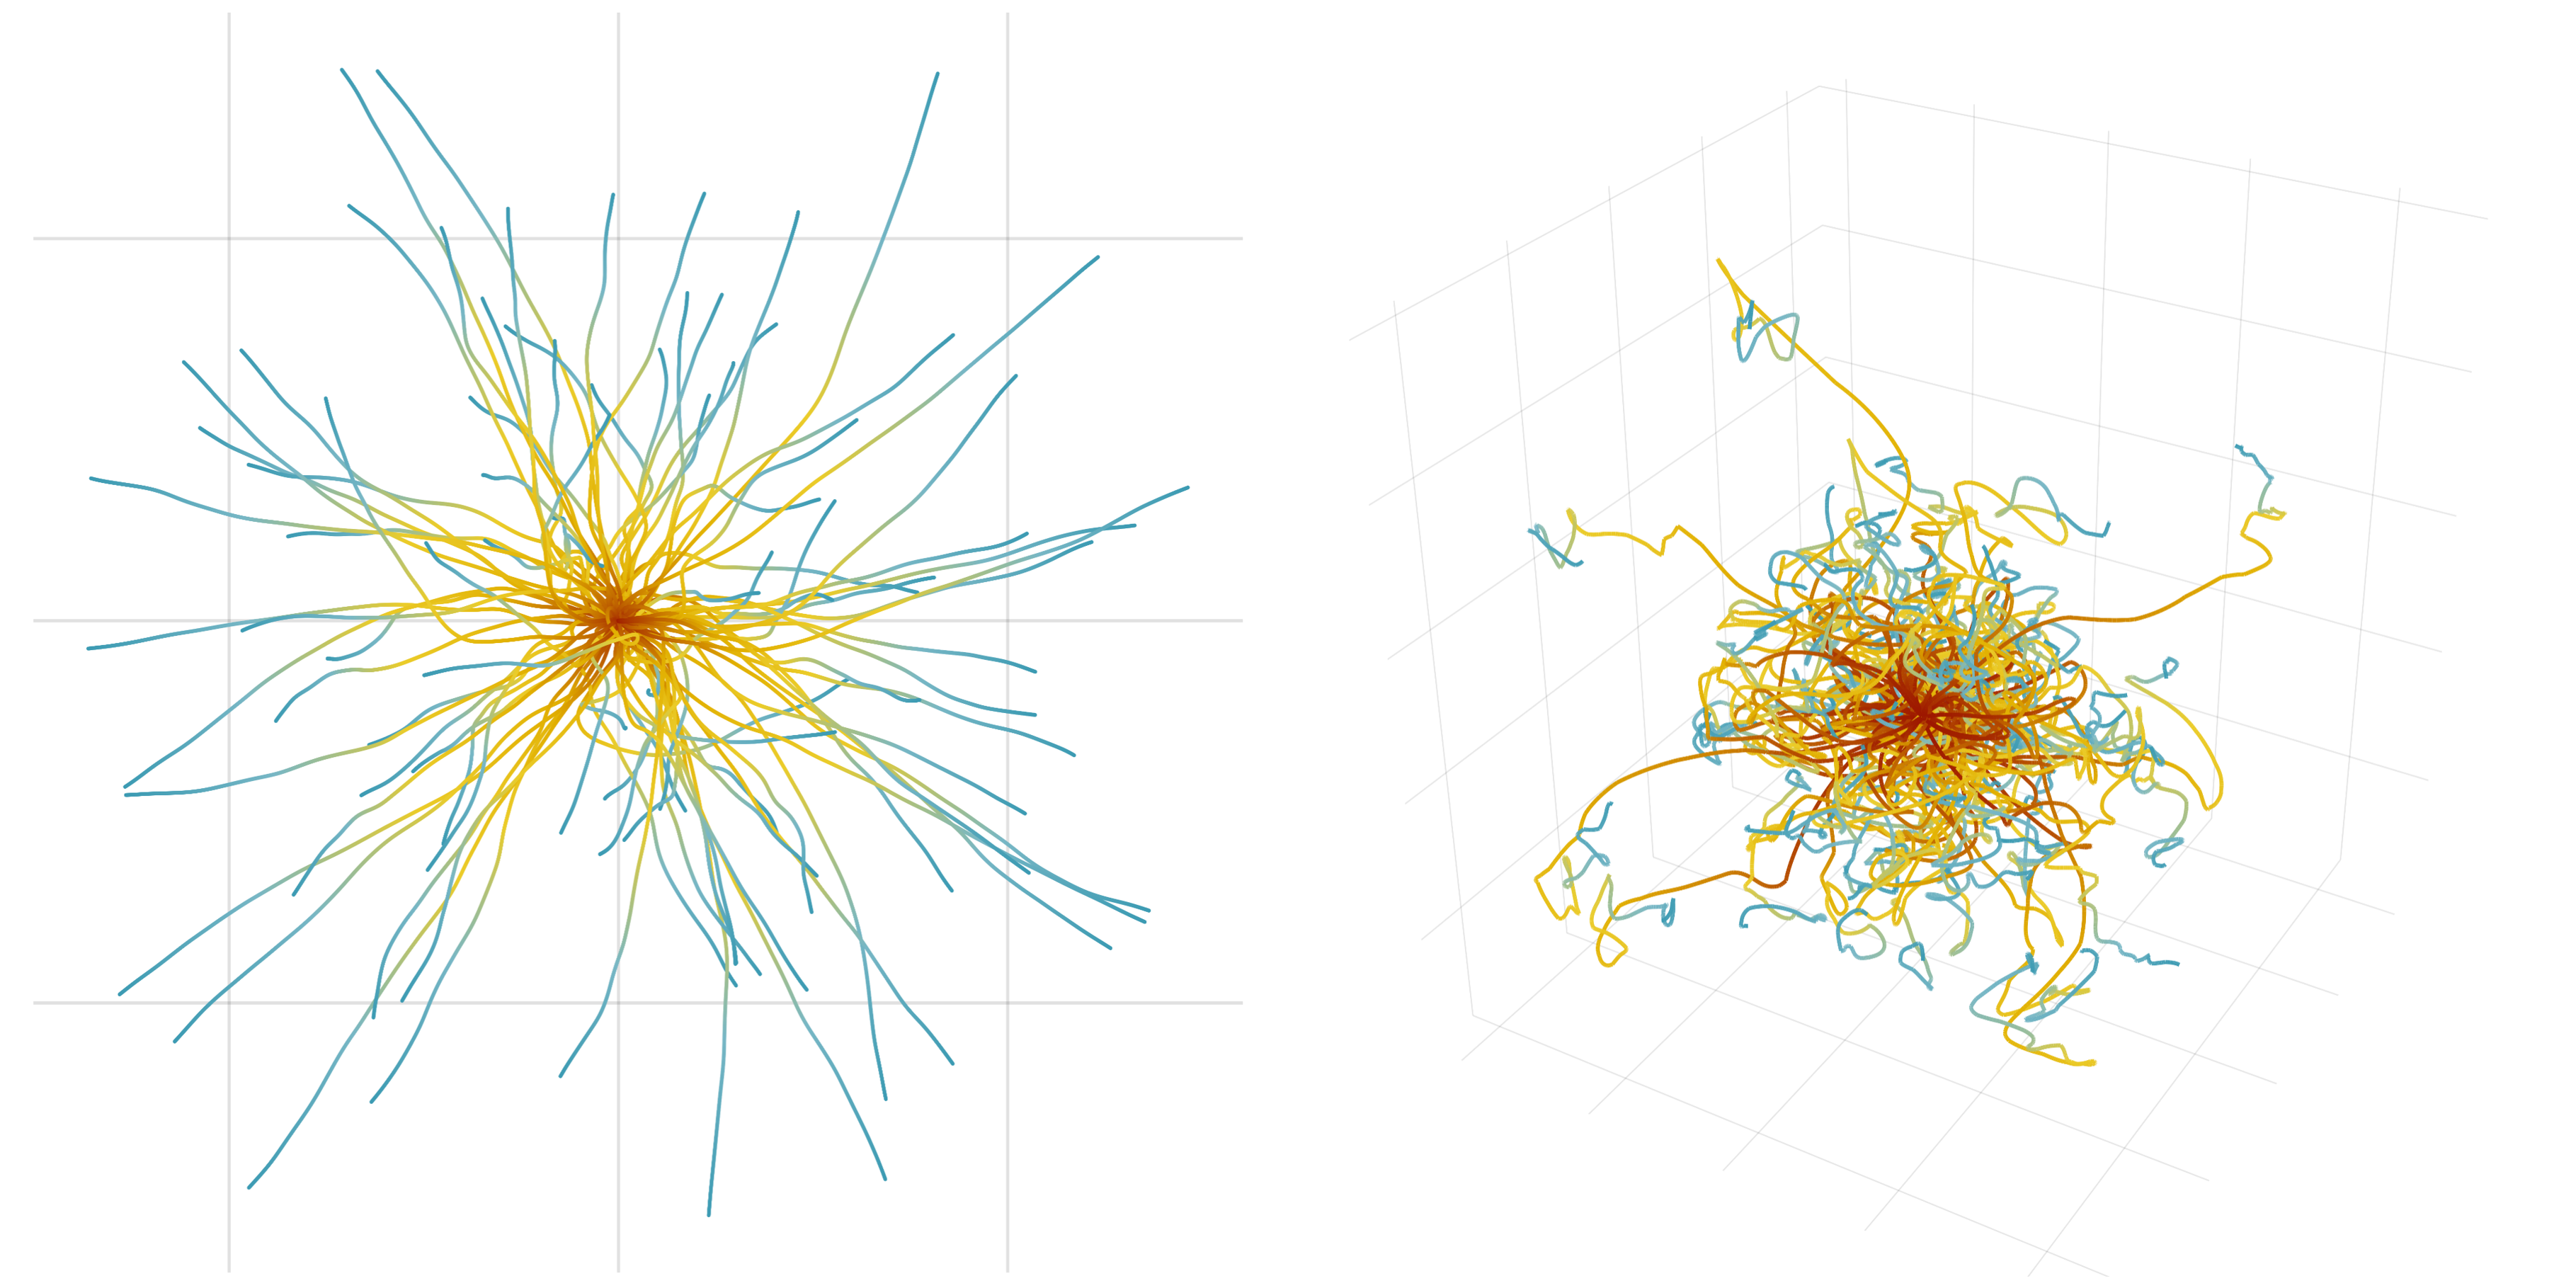
\includegraphics[height=0.7\paperheight]{images/trajectories_cpic.png}} 
%     \\[10pt]  
%    };
% }
% \begin{frame}{Outline}
%     \begin{center}
%         \tableofcontents
%     \end{center}
% \end{frame}
% \setbeamertemplate{background}{}

%%%%%%%%%%%%%%%%%%%%%%%%%%%%%%%%%%%%%%%%%
%%%%%%%%%%%%%%% OUTLINE %%%%%%%%%%%%%%%%%
%%%%%%%%%%%%%%%%%%%%%%%%%%%%%%%%%%%%%%%%%

\begin{frame}
    \frametitle{Outline}
    \vspace{-13pt}
    \begin{center}
        \begin{columns}
            \column{.02\textwidth}
            \column{.6\textwidth}
                \vspace{5pt}
                \begin{center}
                \begin{custombox2}{\large Contents}{starrysecond}
                    \footnotesize
                    \begin{varwidth}{0.89\textwidth}
                    \begin{itemize}\itemsep0em 
                        \setbeamertemplate{itemize item}{\raisebox{0.2em}{\scalebox{0.7}{${\color{starrysecond}\blacktriangleright}$}}} 
                        \item {\bfseries\color{starrysecond}Introduction}: {\scriptsize\itshape hard probes in glasma initial stage}
                        \item {\bfseries\color{starrysecond}Glasma}: {\scriptsize\itshape classical Yang-Mills equations, features}
                        \item {\bfseries\color{starrysecond}Transport in glasma}: {\scriptsize\itshape Wong's equations}
                        \item {\bfseries\color{starrysecond}Transport coefficients}: {\scriptsize\itshape momentum broadening}
                        \item {\bfseries\color{starrysecond}Phenomenology}: {\scriptsize\itshape heavy quark $R_{AA}$, $Q\overline{Q}$ correlations}
                    \end{itemize}
                    \end{varwidth}
                \end{custombox2}
                \vspace{15pt}
                \begin{custombox2}{{\color{jyured}\large Developments}}{lightgray}
                    \footnotesize
                    \begin{varwidth}{0.78\textwidth}
                    \begin{itemize}\itemsep0em 
                        \setbeamertemplate{itemize item}{\raisebox{0.2em}{\scalebox{0.7}{${\color{jyured}\blacktriangleright}$}}} 
                        \item Jet quenching in glasma
                        \item Couple transport in glasma to next stages
                        \item Relevant observables for transport in glasma
                        \item Glasma improvements
                    \end{itemize}
                    \end{varwidth}
                \end{custombox2}
            \end{center}
            \column{.01\textwidth}
            \column{.36\textwidth}
                \begin{center}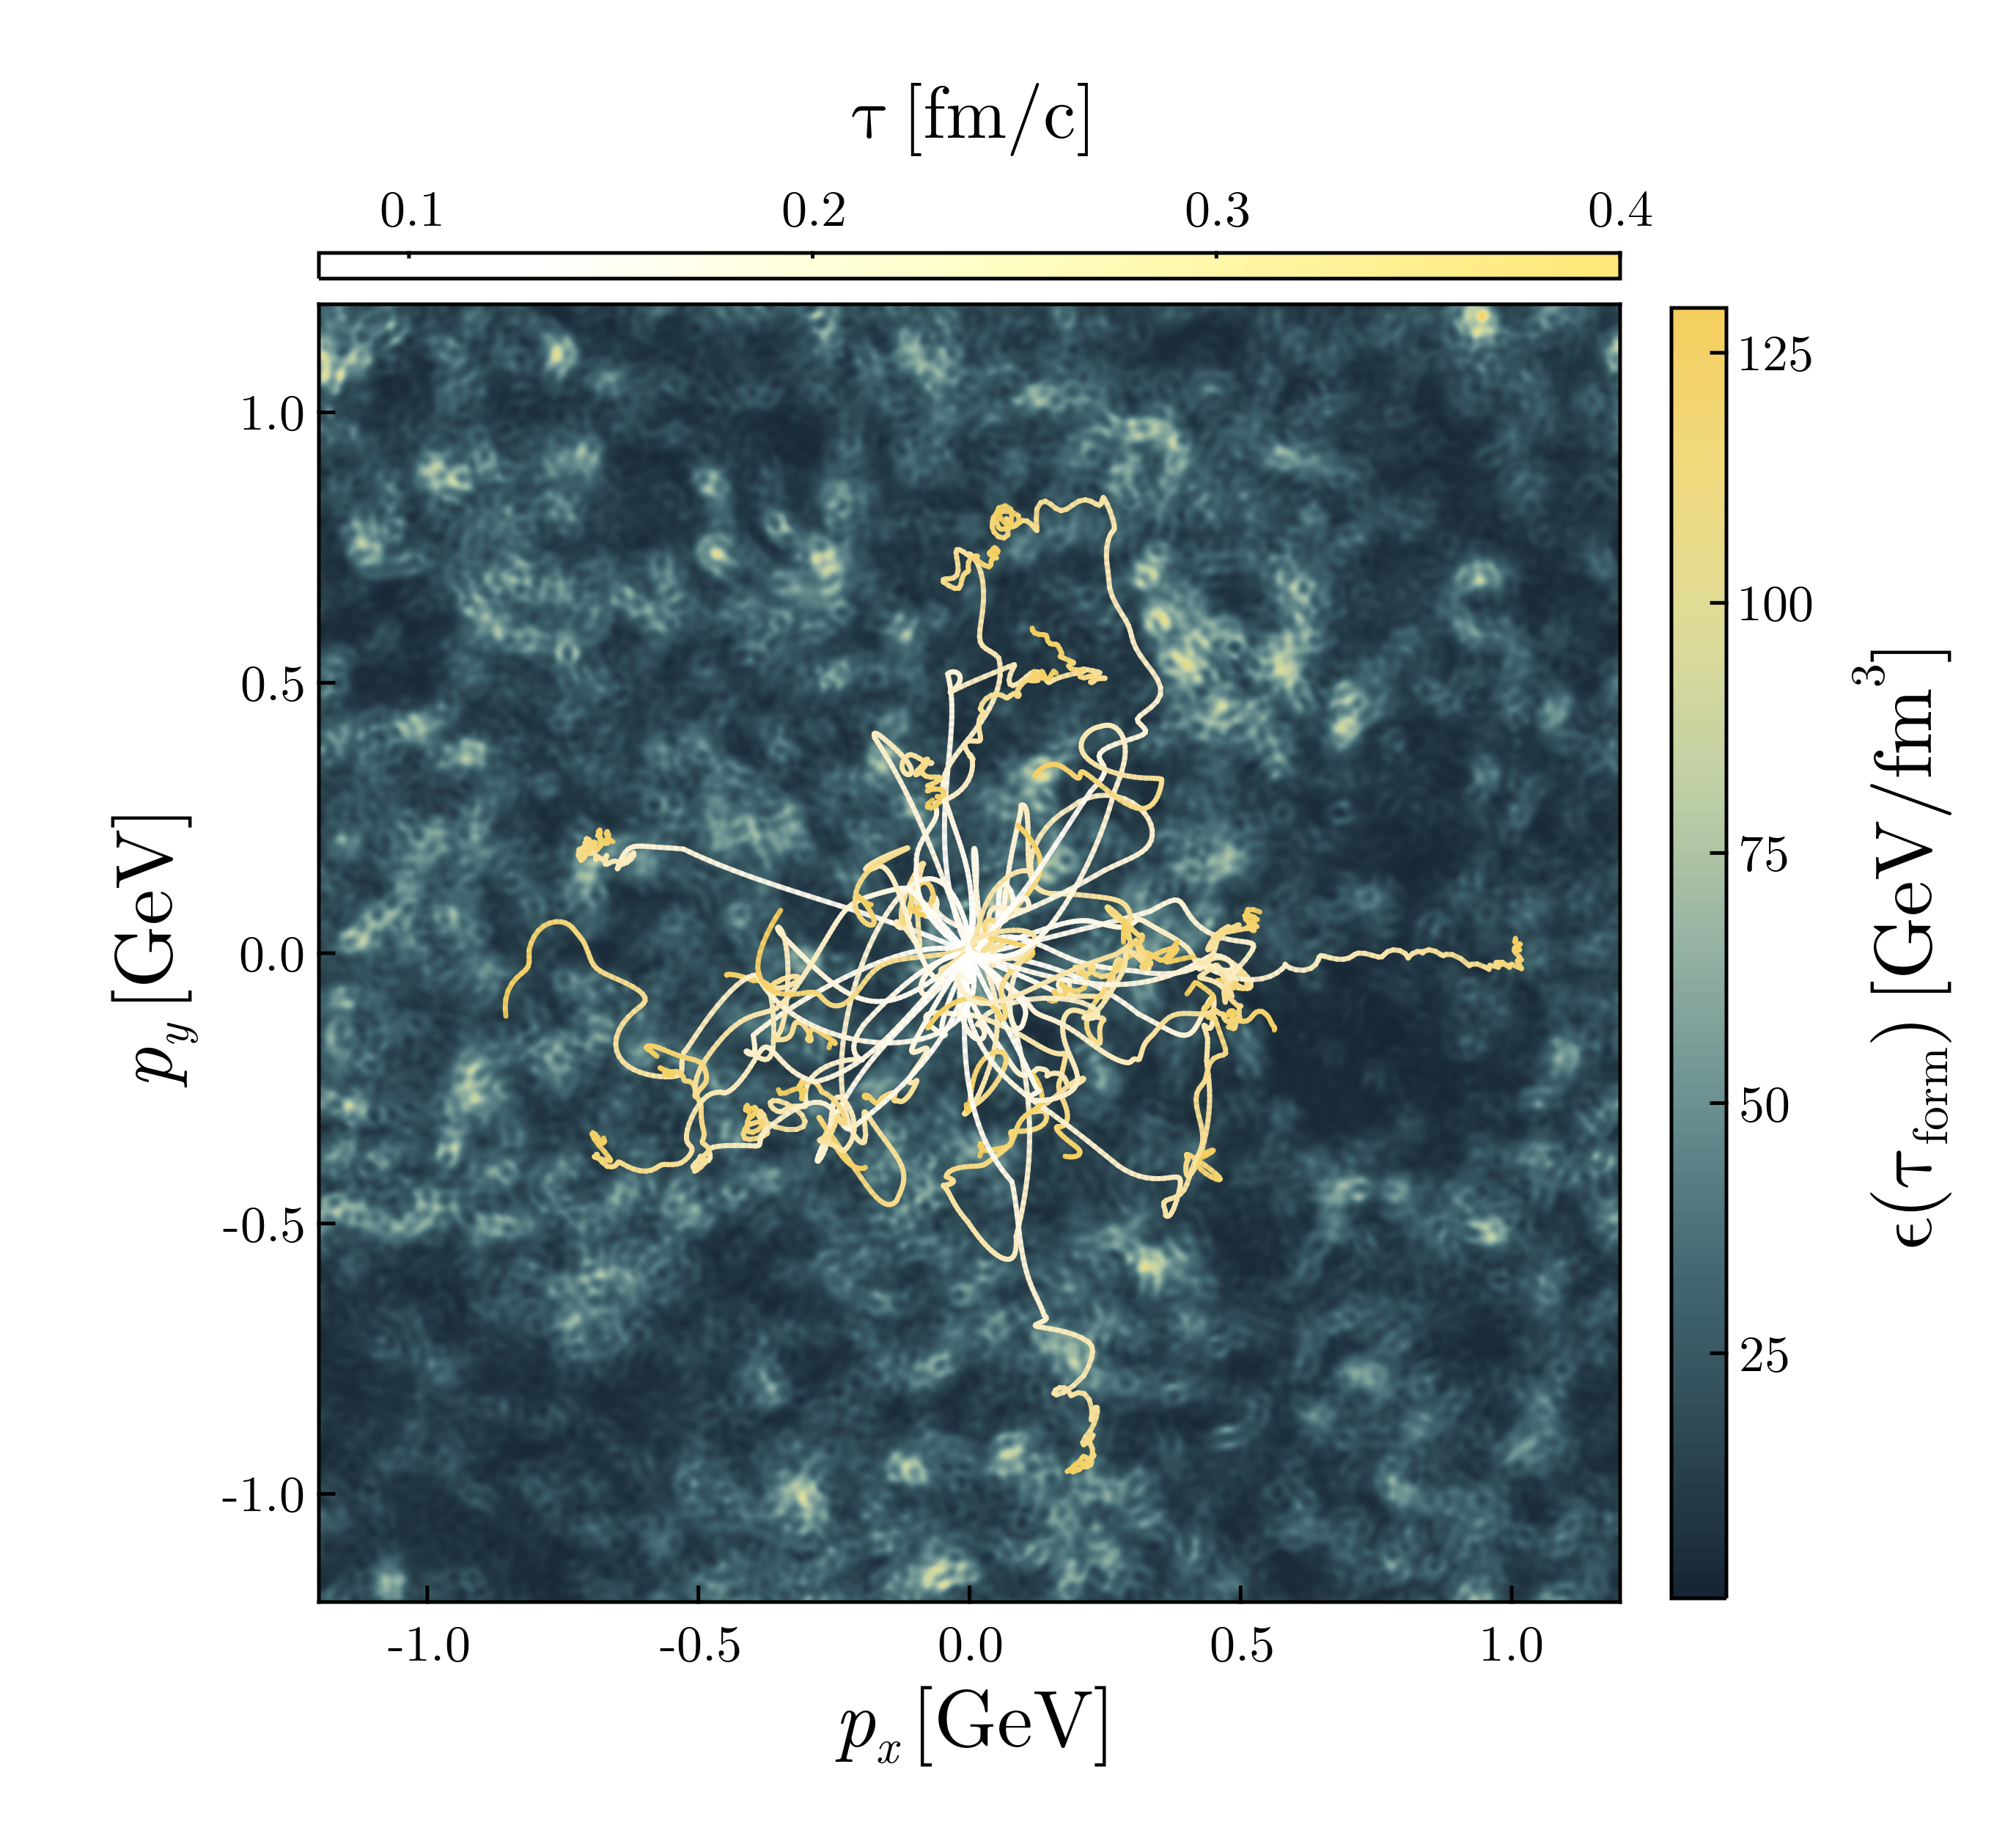
\includegraphics[width=0.9\columnwidth]{images/hqs_trajectories.png}\\[5pt]
                    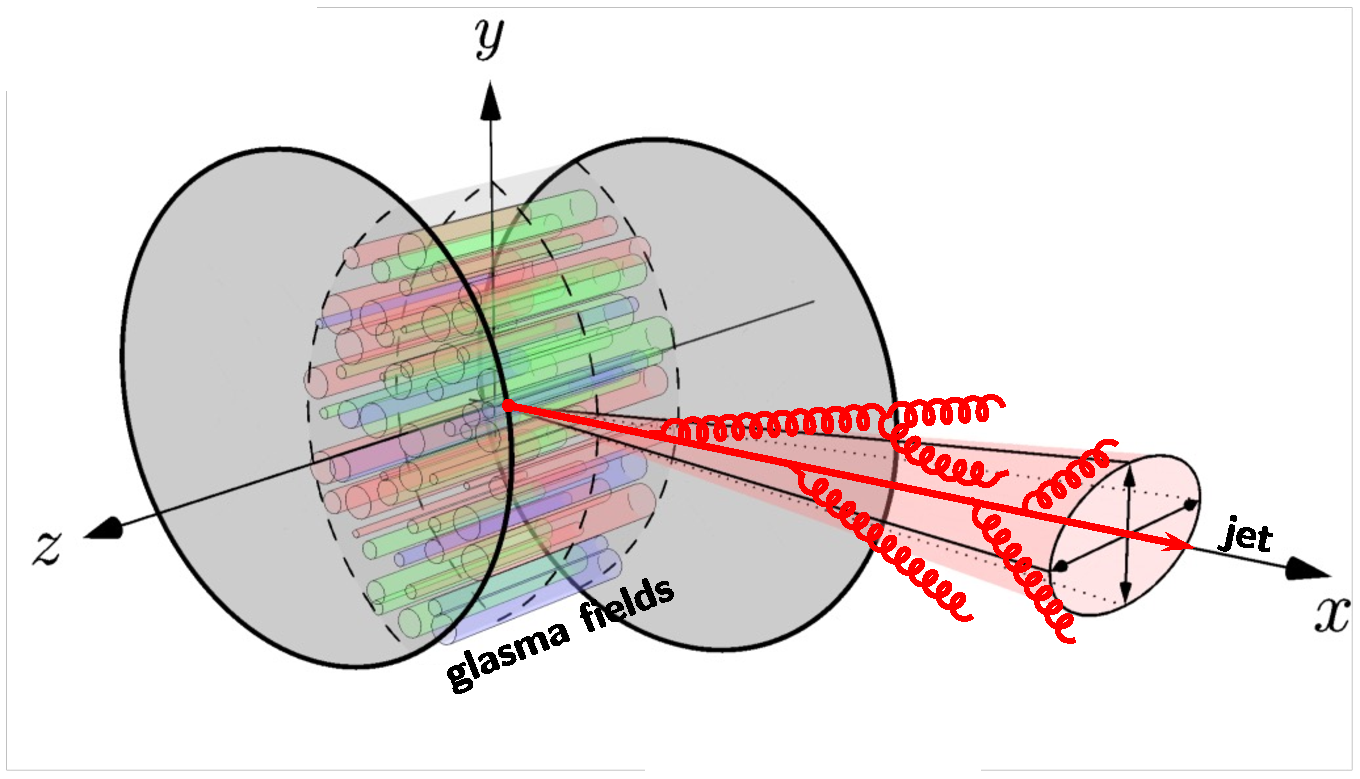
\includegraphics[width=\columnwidth]{images/momentum_broadening_flipped_jetquenched_notext.pdf}\end{center}
            \column{.02\textwidth}
        \end{columns}
    \end{center}
\end{frame}


\setcounter{framenumber}{0}
\setbeamertemplate{footline}[progress bar]
\setbeamercolor{progress bar}{fg=palteal,bg=palteal!40}
\addtobeamertemplate{headline}{}{\vspace{1cm}\hfill\circcounter\hspace*{1cm}}
\addtobeamertemplate{frametitle}{\vspace{-0.8cm}}{}

%%%%%%%%%%%%%%%%%%%%%%%%%%%%%%%%%%%%%%%%%
%%%%%%%%%%%%%%%% SECTION %%%%%%%%%%%%%%%%
%%%%%%%%%%%%%%%%%%%%%%%%%%%%%%%%%%%%%%%%%

\section{Introduction}

%%%%%%%%%%%%%%%%%%%%%%%%%%%%%%%%%%%%%%%%%
%%%%%%%%%%%%%% SUBSECTION %%%%%%%%%%%%%%%
%%%%%%%%%%%%%%%%%%%%%%%%%%%%%%%%%%%%%%%%%

\subsection{Stages}

%%%%%%%%%%%%%%%%%%%%%%%%%%%%%%%%%%%%%%%%%
%%%%%%%%%%%%%%%%% SLIDE %%%%%%%%%%%%%%%%%
%%%%%%%%%%%%%%%%%%%%%%%%%%%%%%%%%%%%%%%%%

\begin{frame}
    \frametitle{Heavy-ion collisions}
    \framesubtitle{Stages at weak coupling}
    \vspace{-15pt}
    \begin{columns}[onlytextwidth,t]
        \column{.02\textwidth}
        \column{.47\textwidth}
            \begin{center}
                \vspace{-5pt}
                \begin{tikzpicture}
                    \node[anchor=south west,inner sep=0] at (0,0) {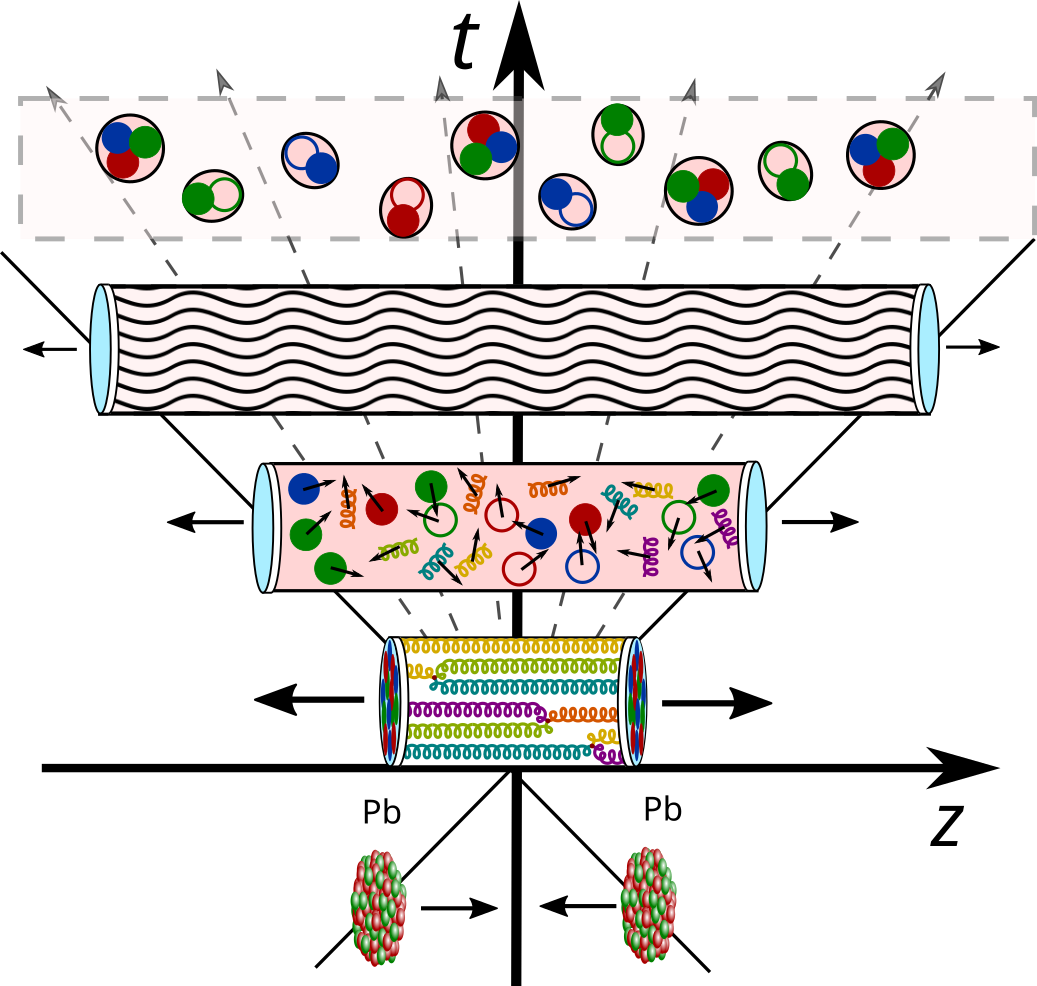
\includegraphics[width=0.95\textwidth]{images/cover_figure_A01.png}};
                \end{tikzpicture}
            \end{center}
        \column{.02\textwidth}
        \column{.47\textwidth}
            \vspace{10pt}
            \begin{center}
            \begin{custombox2}{\color{normal}Collision stages}{lightgray}
                \small
                \begin{varwidth}{0.8\textwidth}
                \begin{itemize}\itemsep0em 
                    \setbeamertemplate{itemize item}{\raisebox{0.2em}{\scalebox{0.7}{${\color{normal}\blacktriangleright}$}}} 
                    \item {Before collision {\scriptsize $\tau\leq 0\,\mathrm{fm/c}$}}\\[1pt]
                        {\color{lightgray}\scriptsize\itshape Gluon field of high-energy nucleus}
                    \setbeamertemplate{itemize item}{\raisebox{0.2em}{\scalebox{0.7}{${\color{palviolet}\blacktriangleright}$}}} \item {{\bfseries\color{palviolet} Initial stage} {\scriptsize $\tau\lesssim
                    0.3\,\mathrm{fm/c}$}}\\[1pt]
                        {\color{lightgray}\scriptsize\itshape {\bfseries\color{palviolet}Glasma strong classical gluon fields}}
                    \setbeamertemplate{itemize item}{\raisebox{0.2em}{\scalebox{0.7}{${\color{normal}\blacktriangleright}$}}} \item Thermalization {\scriptsize$\tau\lesssim
                    1\,\mathrm{fm/c}$}\\[1pt] 
                        {\color{lightgray}\scriptsize\itshape Effective kinetic theory (EKT)} 
                        % \\ {\color{lightgray}\scriptsize Quasiparticle distribution function}
                    \item Equilibration {\scriptsize $\tau\lesssim 10\,\mathrm{fm/c}$}\\[1pt]
                    {\color{lightgray}\scriptsize\itshape Relativistic hydrodynamics} 
                    % \\ {\color{lightgray}\scriptsize Energy-momentum tensor}
                    \item Final stages {\scriptsize $\tau\geq 10\,\mathrm{fm/c}$}\\[1pt]
                    {\color{lightgray}\scriptsize\itshape Particlization, hadronization}
                \end{itemize}
                \end{varwidth}
            \end{custombox2}
            \end{center}
        \column{.02\textwidth}
    \end{columns}
    \blfootnote{\scriptsize Berges, Heller, Mazeliauskas, Venugopalan \href{https://arxiv.org/abs/2005.12299}{{\color{palgold}\texttt{[2005.12299]$^\text{\scalebox{0.9}{\faExternalLink}}$}}} Schlichting, Teaney \href{https://arxiv.org/abs/1908.02113}{{\color{palgold}\texttt{[1908.02113]$^\text{\scalebox{0.9}{\faExternalLink}}$}}}}
    \begin{tikzpicture}[overlay, remember picture]
        \node[anchor=north west] 
        at ([xshift=0.05cm,yshift=-0.05cm]current page.north west) {\begin{talkbox}\scriptsize{\color{destacado}Kurkela$\hspace{1pt}^\text{\scalebox{0.9}{\faComment}}$} {\itshape Mon 14:30$\hspace{1pt}^\text{\scalebox{0.9}{\faClockO}}$} \end{talkbox}};
    \end{tikzpicture}
    \begin{tikzpicture}[overlay, remember picture]
        \node[anchor=north west] 
        at ([xshift=0.05cm,yshift=-0.48cm]current page.north west) {\begin{talkbox}\scriptsize{EKT intro} \end{talkbox}};
    \end{tikzpicture}
\end{frame}

\subsection{Initial stage}

%%%%%%%%%%%%%%%%%%%%%%%%%%%%%%%%%%%%%%%%%
%%%%%%%%%%%%%%%%% SLIDE %%%%%%%%%%%%%%%%%
%%%%%%%%%%%%%%%%%%%%%%%%%%%%%%%%%%%%%%%%%

\begin{frame}[noframenumbering]
    \frametitle{Initial stage of collision}
    % \framesubtitle{Stages at weak coupling}
    \vspace{-15pt}
    \begin{columns}[onlytextwidth,t]
        \column{.02\textwidth}
        \column{.47\textwidth}
            \begin{center}
                \vspace{-5pt}
                \begin{tikzpicture}
                    \node[anchor=south west,inner sep=0] at (0,0) {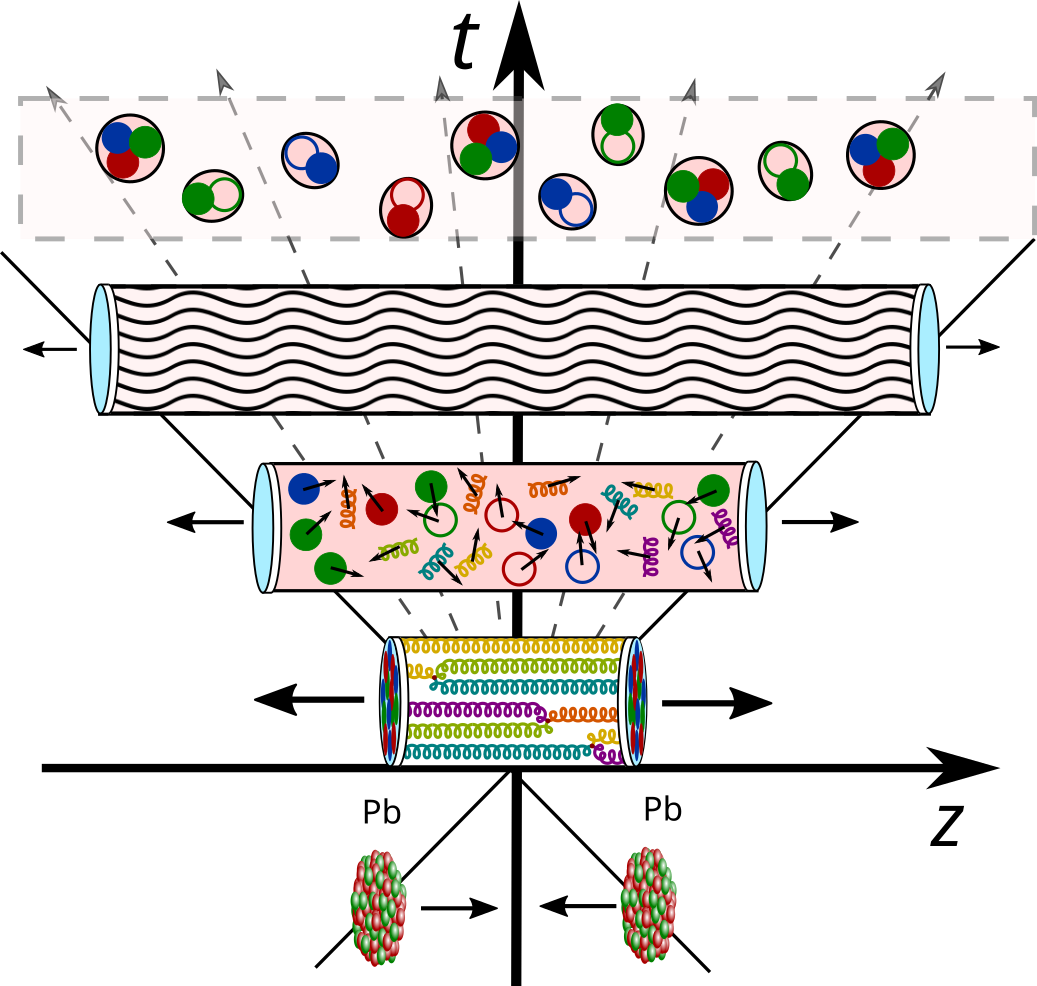
\includegraphics[width=0.95\textwidth]{images/cover_figure_A01.png}};
                    \draw<1>[white, fill=white, fill opacity=0.9] (0.0,2.45) rectangle (6.8,6.5);
                    \draw<1>[palviolet,thick,fill=palviolet,fill opacity=0.1,rounded corners=3pt] (0.1,-0.1) rectangle (6.7,2.45);
                \end{tikzpicture}
            \end{center}
        \column{.02\textwidth}
        \column{.47\textwidth}
            \vspace{7pt}
            \begin{center}
            \begin{custombox2}{Glasma initial stage}{palviolet}
                \small
                \begin{varwidth}{0.76\textwidth}
                \begin{itemize}\itemsep0em 
                    \setbeamertemplate{itemize item}{\raisebox{0.2em}{\scalebox{0.7}{${\color{palviolet}\blacktriangleright}$}}} 
                    \item {\bfseries Color glass condensate}\\[1pt]
                        {\color{lightgray}\scriptsize QCD in the high-energy limit}
                    \item Weakly coupled $\alpha_s\ll 1$
                    \item {\bfseries Classical gluon fields}\\[1pt]
                        {\color{lightgray}\scriptsize Occupation number $\sim 1/\alpha_s\gg 1$}
                    \item {\bfseries Non-perturbative} regime
                    % \item {\bfseries Lattice gauge theory}\\[1pt]
                        % {\color{lightgray}\scriptsize Numerical solution}
                    \item {\bfseries Out-of-equilibrium} medium
                    
                \end{itemize}
                \end{varwidth}
            \end{custombox2}

            \begin{custombox2}{Hard probes}{palteal}
                \small
                \begin{varwidth}{0.68\textwidth}
                \begin{itemize}\itemsep0em 
                    \setbeamertemplate{itemize item}{\raisebox{0.2em}{\scalebox{0.7}{${\color{palteal}\blacktriangleright}$}}} 
                    \item Jets and heavy quarks\\[1pt]
                    {\color{lightgray}\scriptsize Produced in the initial stage}
                    % {\color{lightgray}\scriptsize Kinematics large $E$/large $m$}
                \end{itemize}
                \end{varwidth}
            \end{custombox2}
            \end{center}
        \column{.02\textwidth}
    \end{columns}
    \vspace{-5pt}
    \blfootnote{\scriptsize Lappi \href{https://arxiv.org/abs/hep-ph/0606207}{{\color{palviolet}\texttt{[hep-ph/0606207]}$^\text{\scalebox{0.9}{\faExternalLink}}$}} Gelis \href{https://arxiv.org/abs/1211.3327}{{\color{palviolet}\texttt{[1211.3327]}$^\text{\scalebox{0.9}{\faExternalLink}}$}}}
    \begin{tikzpicture}[overlay, remember picture]
        \node[anchor=north west] 
        at ([xshift=0.05cm,yshift=-0.05cm]current page.north west) {\begin{talkbox}\scriptsize{\color{destacado}Ruggieri$\hspace{1pt}^\text{\scalebox{0.9}{\faComment}}$} {\itshape Mon 11:00$\hspace{1pt}^\text{\scalebox{0.9}{\faClockO}}$} \end{talkbox}};
    \end{tikzpicture}
    \begin{tikzpicture}[overlay, remember picture]
        \node[anchor=north west] 
        at ([xshift=0.05cm,yshift=-0.48cm]current page.north west) {\begin{talkbox}\scriptsize{Glasma intro} \end{talkbox}};
    \end{tikzpicture}
    \begin{tikzpicture}[overlay, remember picture]
        \node[anchor=north west] 
        at ([xshift=0.05cm,yshift=-1.05cm]current page.north west) {\begin{talkbox}\scriptsize{\color{destacado}Montero$\hspace{1pt}^\text{\scalebox{0.9}{\faComment}}$} {\itshape Fri 9:45$\hspace{1pt}^\text{\scalebox{0.9}{\faClockO}}$} \end{talkbox}};
    \end{tikzpicture}
    \begin{tikzpicture}[overlay, remember picture]
        \node[anchor=north west] 
        at ([xshift=0.05cm,yshift=-1.48cm]current page.north west) {\begin{talkbox}\scriptsize{Electromagnetic probes} \end{talkbox}};
    \end{tikzpicture}
\end{frame}


%%%%%%%%%%%%%%%%%%%%%%%%%%%%%%%%%%%%%%%%%
%%%%%%%%%%%%%% SUBSECTION %%%%%%%%%%%%%%%
%%%%%%%%%%%%%%%%%%%%%%%%%%%%%%%%%%%%%%%%%

\subsection{Hard probes}

%%%%%%%%%%%%%%%%%%%%%%%%%%%%%%%%%%%%%%%%%
%%%%%%%%%%%%%%%%% SLIDE %%%%%%%%%%%%%%%%%
%%%%%%%%%%%%%%%%%%%%%%%%%%%%%%%%%%%%%%%%%

\setbeamertemplate{background}{
\tikz[overlay,remember picture] \node[at=(current page.center), align=center] {\\[10pt]
{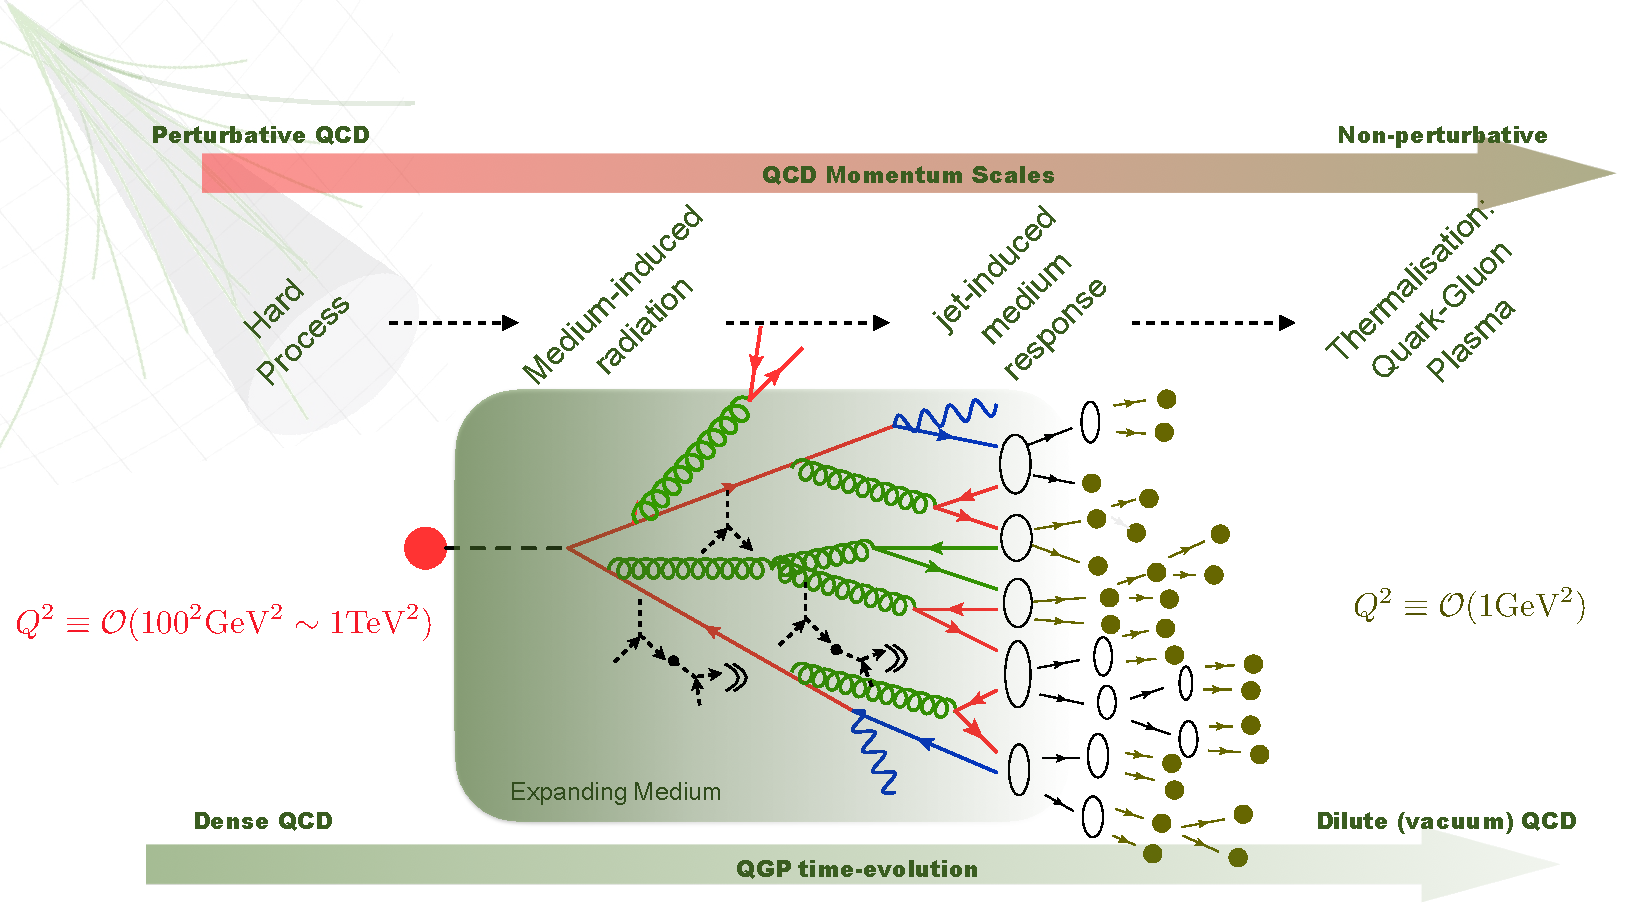
\includegraphics[height=0.8\paperheight]{images/Holmganga_jets_Liliana-scales.pdf}}};
}
\begin{frame}
    \frametitle{Jets as probes}
    \framesubtitle{Stages and scales of interest}
    \blfootnote{\scriptsize Apolinario \href{https://indico.cern.ch/event/1385550/}{{\color{jyured}\texttt{[CERN 24]$^\text{\scalebox{0.9}{\faExternalLink}}$}}}}
    \begin{tikzpicture}[overlay, remember picture]
        \node[anchor=north west] 
        at ([xshift=0.05cm,yshift=-0.05cm]current page.north west) {\begin{talkbox}\scriptsize{\color{destacado}Apolinario$\hspace{1pt}^\text{\scalebox{0.9}{\faComment}}$} {\itshape Mon 9:00$\hspace{1pt}^\text{\scalebox{0.9}{\faClockO}}$} \end{talkbox}};
    \end{tikzpicture}
    \begin{tikzpicture}[overlay, remember picture]
        \node[anchor=north west] 
        at ([xshift=0.05cm,yshift=-0.48cm]current page.north west) {\begin{talkbox}\scriptsize{Jets intro} \end{talkbox}};
    \end{tikzpicture}
\end{frame}
\setbeamertemplate{background}{}

%%%%%%%%%%%%%%%%%%%%%%%%%%%%%%%%%%%%%%%%%
%%%%%%%%%%%%%%%%% SLIDE %%%%%%%%%%%%%%%%%
%%%%%%%%%%%%%%%%%%%%%%%%%%%%%%%%%%%%%%%%%

\setbeamertemplate{background}{
\tikz[overlay,remember picture] \node[at=(current page.center), align=left] {\\[-5pt]
{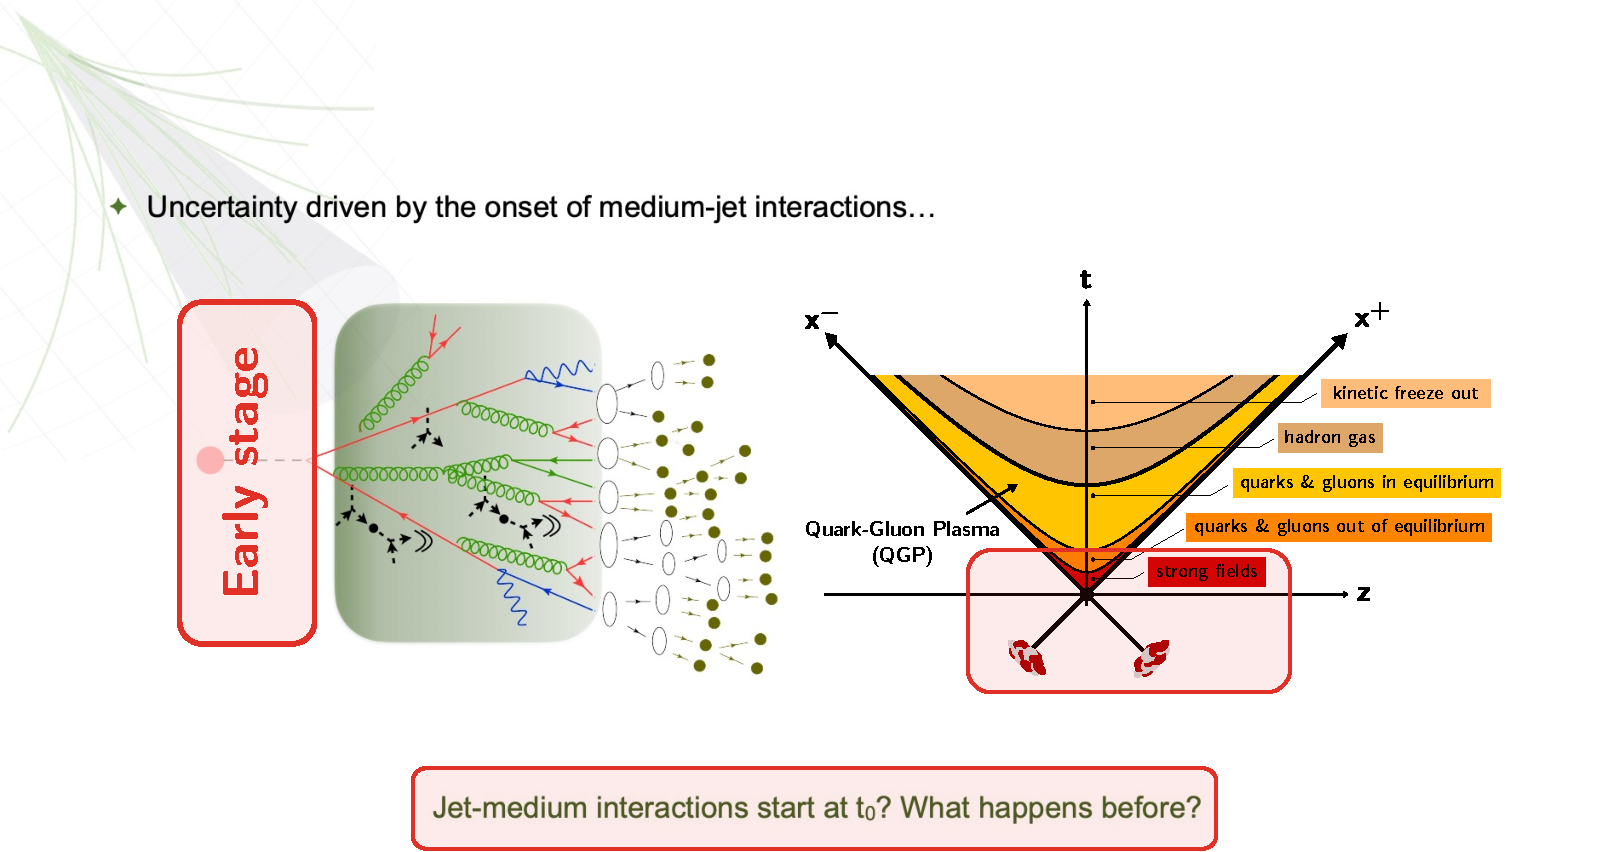
\includegraphics[height=0.8\paperheight]{images/LApolinario_HP23-modelling-early_v2.pdf}}};
}
\begin{frame}[noframenumbering]
    \frametitle{Jets as probes of {\color{jyured}early stages}}
    % \framesubtitle{Stages and scales of interest}
    \blfootnote{\scriptsize Apolinario \href{https://indico.uni-muenster.de/event/1409/contributions/2412/}{{\color{jyured}\texttt{[Hard Probes 23]$^\text{\scalebox{0.9}{\faExternalLink}}$}}} adapted}
    \begin{tikzpicture}[overlay, remember picture]
        \node[anchor=north west] 
        at ([xshift=0.05cm,yshift=-0.05cm]current page.north west) {\begin{talkbox}\scriptsize{\color{destacado}López$\hspace{1pt}^\text{\scalebox{0.9}{\faComment}}$} {\itshape Mon 9:45$\hspace{1pt}^\text{\scalebox{0.9}{\faClockO}}$} \end{talkbox}};
    \end{tikzpicture}
    \begin{tikzpicture}[overlay, remember picture]
        \node[anchor=north west] 
        at ([xshift=0.05cm,yshift=-0.48cm]current page.north west) {\begin{talkbox}\scriptsize{Jets in early stage} \end{talkbox}};
    \end{tikzpicture}
    \begin{tikzpicture}[overlay, remember picture]
        \node[anchor=south east] 
        at ([xshift=-0.05cm,yshift=1.63cm]current page.south east) {\begin{talkbox}\scriptsize{\color{destacado}Silvia$\hspace{1pt}^\text{\scalebox{0.9}{\faComment}}$} {\itshape Wed 12:30$\hspace{1pt}^\text{\scalebox{0.9}{\faClockO}}$} \end{talkbox}};
    \end{tikzpicture}
    \begin{tikzpicture}[overlay, remember picture]
        \node[anchor=south east] 
        at ([xshift=-0.05cm,yshift=1.2cm]current page.south east) {\begin{talkbox}\scriptsize{$q\overline{q}$ antenna in early stage} \end{talkbox}};
    \end{tikzpicture}
    \begin{tikzpicture}[overlay, remember picture]
        \node[anchor=south east] 
        at ([xshift=-0.05cm,yshift=0.58cm]current page.south east) {\begin{talkbox}\scriptsize{\color{destacado}Adhya$\hspace{1pt}^\text{\scalebox{0.9}{\faComment}}$} {\itshape Thu 12:30$\hspace{1pt}^\text{\scalebox{0.9}{\faClockO}}$} \end{talkbox}};
    \end{tikzpicture}
    \begin{tikzpicture}[overlay, remember picture]
        \node[anchor=south east] 
        at ([xshift=-0.05cm,yshift=0.16cm]current page.south east) {\begin{talkbox}\scriptsize{Jet sensitivity to early stage} \end{talkbox}};
    \end{tikzpicture}
\end{frame}
\setbeamertemplate{background}{}

%%%%%%%%%%%%%%%%%%%%%%%%%%%%%%%%%%%%%%%%%
%%%%%%%%%%%%%%%%% SLIDE %%%%%%%%%%%%%%%%%
%%%%%%%%%%%%%%%%%%%%%%%%%%%%%%%%%%%%%%%%%

\begin{frame}
    \frametitle{Heavy quarks as probes}
    \framesubtitle{Approaches and kinematic regimes}

    \begin{columns}[onlytextwidth,t]
        \column{.02\textwidth}
        \column{.57\textwidth}
            \vspace{-20pt}
            \begin{center}
                \begin{tikzpicture}
                    \node[anchor=south west,inner sep=0] at (0,0) {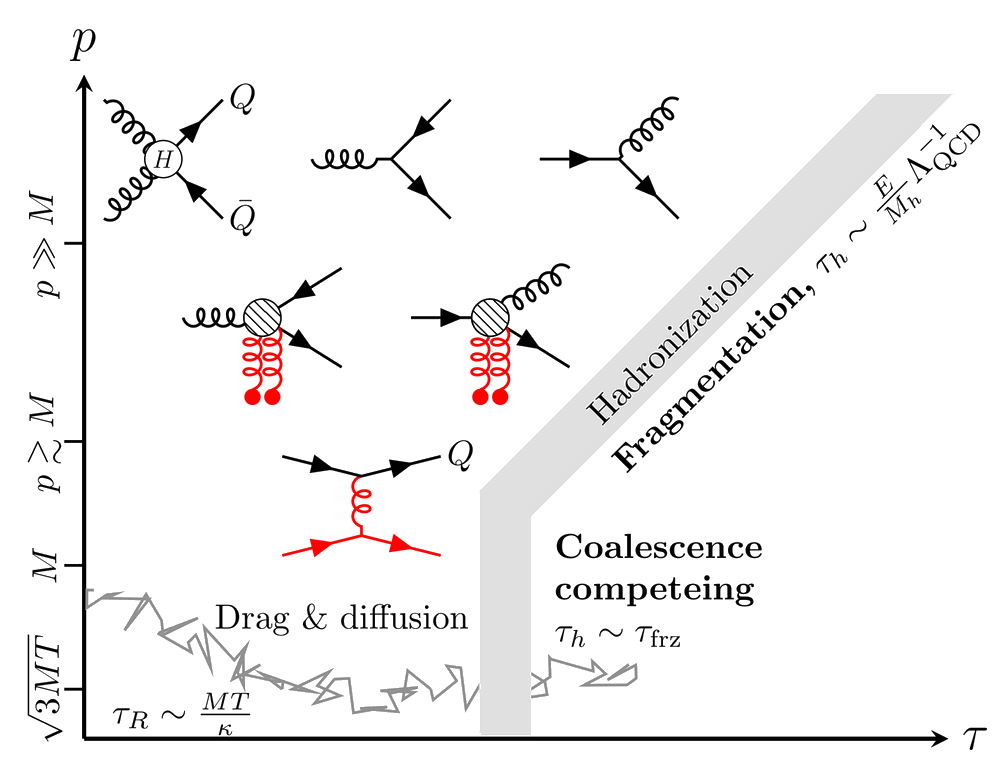
\includegraphics[width=0.95\textwidth]{images/HP24-Weiyao-Ke-HF-Theory-2-crop-white.png}};
                \end{tikzpicture}
            \end{center}
        \column{.02\textwidth}
        \column{.37\textwidth}
        \vspace{0pt}
        \begin{center}
            \begin{custombox2}{\color{normal}Approaches}{lightgray}
                \small
                \begin{varwidth}{0.85\textwidth}
                \begin{itemize}\itemsep0em 
                    \setbeamertemplate{itemize item}{\raisebox{0.2em}{\scalebox{0.7}{${\color{normal}\blacktriangleright}$}}} 
                    \item pQCD production\\[1pt]
                        {\color{lightgray}\scriptsize FONLL and GM-VFNS at NLO+NLL accuracy}
                    \item Transport models\\[1pt]
                        {\color{lightgray}\scriptsize Boltzmann, Langevin, Fokker-Planck equations}
                    \item Hadronization\\[1pt]
                        {\color{lightgray}\scriptsize Fragmentation + coalescence}  
                \end{itemize}
                \end{varwidth}
            \end{custombox2}
            \end{center}
        \column{.02\textwidth}
    \end{columns}
    \vspace{-5pt}    
    \blfootnote{\scriptsize Ke \href{https://indico.cern.ch/event/1339555/contributions/6038190/}{{\color{jyured}\texttt{[Hard Probes 24]$^\text{\scalebox{0.9}{\faExternalLink}}$}}}}
    \begin{tikzpicture}[overlay, remember picture]
        \node[anchor=north west] 
        at ([xshift=0.05cm,yshift=-0.05cm]current page.north west) {\begin{talkbox}\scriptsize{\color{destacado}Greco$\hspace{1pt}^\text{\scalebox{0.9}{\faComment}}$} {\itshape Tue 15:15$\hspace{1pt}^\text{\scalebox{0.9}{\faClockO}}$} \end{talkbox}};
    \end{tikzpicture}
    \begin{tikzpicture}[overlay, remember picture]
        \node[anchor=north west] 
        at ([xshift=0.05cm,yshift=-0.48cm]current page.north west) {\begin{talkbox}\scriptsize{HQs transport} \end{talkbox}};
    \end{tikzpicture}
    \begin{tikzpicture}[overlay, remember picture]
        \node[anchor=south east] 
        at ([xshift=-0.05cm,yshift=1cm]current page.south east) {\begin{talkbox}\scriptsize{\color{destacado}Scheihing$\hspace{1pt}^\text{\scalebox{0.9}{\faComment}}$} {\itshape Wed 9:45$\hspace{1pt}^\text{\scalebox{0.9}{\faClockO}}$} \end{talkbox}};
    \end{tikzpicture}
    \begin{tikzpicture}[overlay, remember picture]
        \node[anchor=south east] 
        at ([xshift=-0.05cm,yshift=0.58cm]current page.south east) {\begin{talkbox}\scriptsize{\color{destacado}Du Plessis$\hspace{1pt}^\text{\scalebox{0.9}{\faComment}}$} {\itshape Wed 16:00$\hspace{1pt}^\text{\scalebox{0.9}{\faClockO}}$} \end{talkbox}};
    \end{tikzpicture}
    \begin{tikzpicture}[overlay, remember picture]
        \node[anchor=south east] 
        at ([xshift=-0.05cm,yshift=0.15cm]current page.south east) {\begin{talkbox}\scriptsize{HQs at strong coupling} \end{talkbox}};
    \end{tikzpicture}
\end{frame}

%%%%%%%%%%%%%%%%%%%%%%%%%%%%%%%%%%%%%%%%%
%%%%%%%%%%%%%%%%% SLIDE %%%%%%%%%%%%%%%%%
%%%%%%%%%%%%%%%%%%%%%%%%%%%%%%%%%%%%%%%%%

\begin{frame}[noframenumbering]
    \frametitle{Heavy quarks as probes of {\color{jyured}early stages}}
    % \framesubtitle{Recent focus on the early stage}

    \begin{center}
        \begin{tikzpicture}
            \node[anchor=south west,inner sep=0] at (0,0) {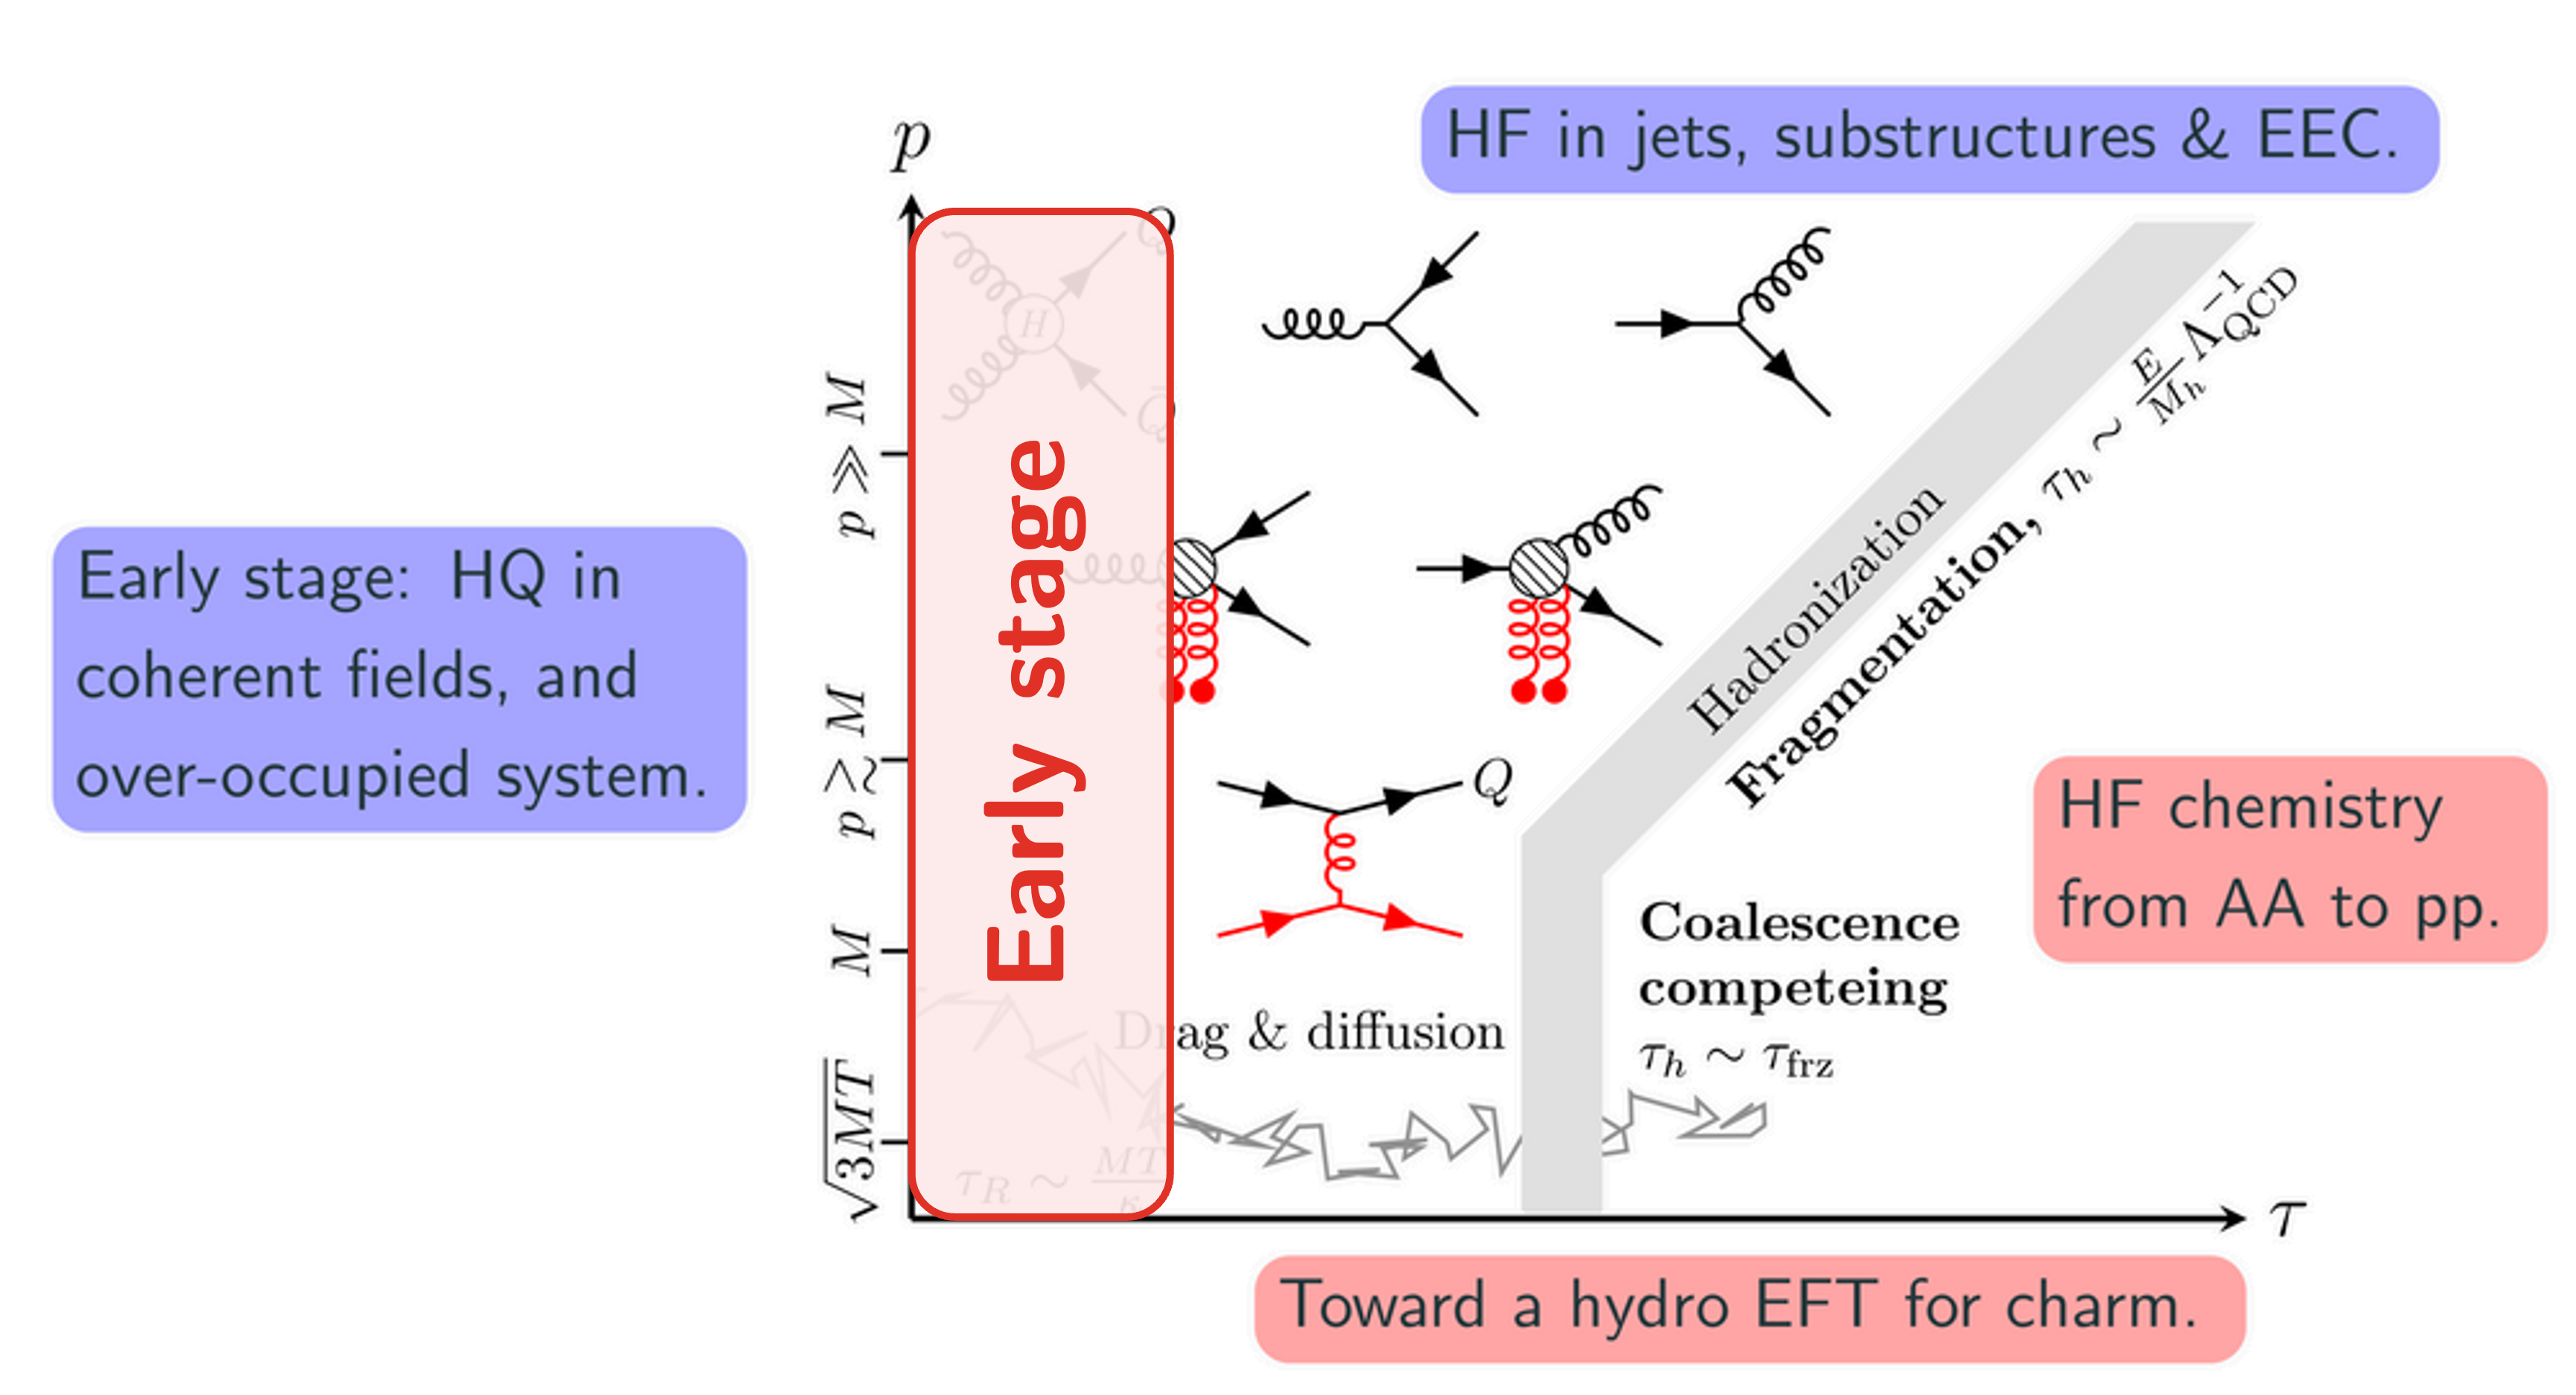
\includegraphics[width=0.8\textwidth]{images/HP24-Weiyao-Ke-HF-Theory-28-crop-white-edit.png}};
            % \draw<1>[palgold,thick,fill=palgold,fill opacity=0.1,rounded corners=3pt] (0.0,4) rectangle (\textheight-0.5cm,4.0) node[opacity=1.0, pos=0, anchor=center, xshift=0.0\linewidth,text width=2cm,align=center]{{\Large\color{palgold}\bfseries This talk}};
            % \draw<1>[white, fill=white, fill opacity=0.9] (4.3,0.85) rectangle (5.4,5.5);
            % \draw<1>[red,thick,fill=red,fill opacity=0.1,rounded corners=3pt] (4.3,0.85) rectangle (5.4,5.5) node[opacity=1.0, pos=0.5, rotate=90, anchor=center, xshift=0.0 ,text width=6.2cm,align=center] {{\Large\color{jyured} Early stage}};
        \end{tikzpicture}
    \end{center}
    \vspace{-10pt}    
    \blfootnote{\scriptsize Ke \href{https://indico.cern.ch/event/1339555/contributions/6038190/}{{\color{jyured}\texttt{[Hard Probes 24]$^\text{\scalebox{0.9}{\faExternalLink}}$}}} adapted}
    \begin{tikzpicture}[overlay, remember picture]
        \node[anchor=north west] 
        at ([xshift=0.05cm,yshift=-1.6cm]current page.north west) {\begin{talkbox}\scriptsize{\color{destacado}Ruggieri$\hspace{1pt}^\text{\scalebox{0.9}{\faComment}}$} {\itshape Mon 11:00$\hspace{1pt}^\text{\scalebox{0.9}{\faClockO}}$} \end{talkbox}};
    \end{tikzpicture}
    \begin{tikzpicture}[overlay, remember picture]
        \node[anchor=north west] 
        at ([xshift=0.05cm,yshift=-2.03cm]current page.north west) {\begin{talkbox}\scriptsize{HQs in glasma} \end{talkbox}};
    \end{tikzpicture}
    \begin{tikzpicture}[overlay, remember picture]
        \node[anchor=north west] 
        at ([xshift=0.05cm,yshift=-5.6cm]current page.north west) {\begin{talkbox}\scriptsize{\color{destacado}Sharma$\hspace{1pt}^\text{\scalebox{0.9}{\faComment}}$} {\itshape Fri 9:00$\hspace{1pt}^\text{\scalebox{0.9}{\faClockO}}$} \end{talkbox}};
    \end{tikzpicture}
    \begin{tikzpicture}[overlay, remember picture]
        \node[anchor=north west] 
        at ([xshift=0.05cm,yshift=-6.03cm]current page.north west) {\begin{talkbox}\scriptsize{\color{destacado}Pandey$\hspace{1pt}^\text{\scalebox{0.9}{\faComment}}$} {\itshape Wed 15:45$\hspace{1pt}^\text{\scalebox{0.9}{\faClockO}}$} \end{talkbox}};
    \end{tikzpicture}
    \begin{tikzpicture}[overlay, remember picture]
        \node[anchor=north west] 
        at ([xshift=0.05cm,yshift=-6.47cm]current page.north west) {\begin{talkbox}\scriptsize{HQs in overoccupied plasma} \end{talkbox}};
    \end{tikzpicture}
\end{frame}



%%%%%%%%%%%%%%%%%%%%%%%%%%%%%%%%%%%%%%%%%
%%%%%%%%%%%%%%%% SECTION %%%%%%%%%%%%%%%%
%%%%%%%%%%%%%%%%%%%%%%%%%%%%%%%%%%%%%%%%%

\section{Glasma fields}

%%%%%%%%%%%%%%%%%%%%%%%%%%%%%%%%%%%%%%%%%
%%%%%%%%%%%%%%%%% SLIDE %%%%%%%%%%%%%%%%%
%%%%%%%%%%%%%%%%%%%%%%%%%%%%%%%%%%%%%%%%%

\setbeamertemplate{background}{
\tikz[overlay,remember picture] \node[opacity=0.1, at=(current page.center), align=center] {\\[10pt]
{\transparent{0.2}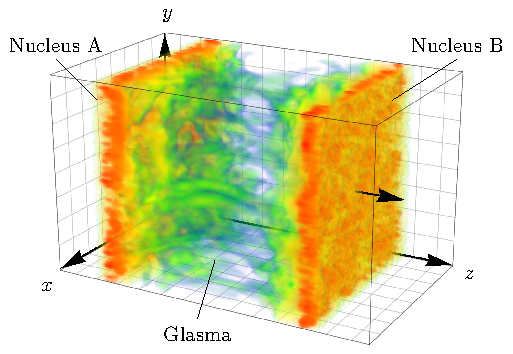
\includegraphics[height=0.8\paperheight]{images/fig1_overview.pdf}}};
}
\begin{frame}[plain,noframenumbering]{}
    \begin{center}
        \vspace{1cm}
        {\large\color{normal}Initial stage of pre-equilibrium}\\[0.3cm]
        {\huge\color{destacado}The glasma}
    \end{center}
\end{frame}
\setbeamertemplate{background}{}

%%%%%%%%%%%%%%%%%%%%%%%%%%%%%%%%%%%%%%%%%
%%%%%%%%%%%%%%%%% SLIDE %%%%%%%%%%%%%%%%%
%%%%%%%%%%%%%%%%%%%%%%%%%%%%%%%%%%%%%%%%%

\setbeamertemplate{background}{
\tikz[overlay,remember picture] \node[at=(current page.center), align=center] {\\[10pt]
{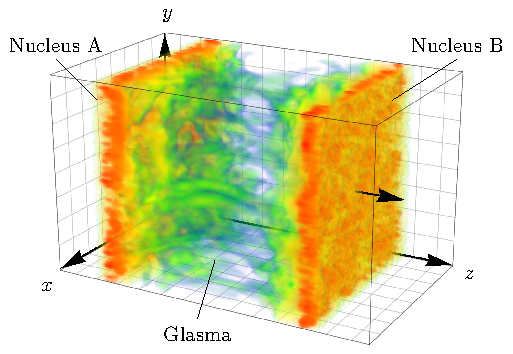
\includegraphics[height=0.7\paperheight]{images/fig1_overview.pdf}}};
}
\begin{frame}[plain,noframenumbering]
    \frametitle{\\ Glasma color fields}
    \blfootnote{\scriptsize Ipp, Müller  \href{https://arxiv.org/abs/1703.00017}{{\color{palgold}\texttt{[1703.00017]}$^\text{\scalebox{0.9}{\faExternalLink}}$}}}
\end{frame}
\setbeamertemplate{background}{}

%%%%%%%%%%%%%%%%%%%%%%%%%%%%%%%%%%%%%%%%%
%%%%%%%%%%%%%% SUBSECTION %%%%%%%%%%%%%%%
%%%%%%%%%%%%%%%%%%%%%%%%%%%%%%%%%%%%%%%%%

\subsection{CGC}

%%%%%%%%%%%%%%%%%%%%%%%%%%%%%%%%%%%%%%%%%
%%%%%%%%%%%%%%%%% SLIDE %%%%%%%%%%%%%%%%%
%%%%%%%%%%%%%%%%%%%%%%%%%%%%%%%%%%%%%%%%%

\setbeamertemplate{itemize item}{\raisebox{0.2em}{\scalebox{0.7}{${\color{normal}\blacktriangleright}$}}} 

\begin{frame}
    \frametitle{Color glass condensate}
    \framesubtitle{QCD at high energy and glasma fields}
    \vspace{-15pt}
    \begin{columns}[onlytextwidth,t]
       \column{.033\textwidth}
       \column{.35\textwidth}

            \begin{center}
                \footnotesize\color{lightgray}A high-energy nucleus contains \\ large numbers of {\bfseries\color{palviolet}soft gluons}
            \end{center}
            % \begin{itemize}\itemsep0em 
            %     \footnotesize\color{lightgray}
            %     \setbeamertemplate{itemize item}{\raisebox{0.2em}{\scalebox{0.6}{${\color{lightgray}\blacktriangleright}$}}}
            %     \item A high-energy nucleus contains mostly {\bfseries\color{palviolet}soft gluons}
            % \end{itemize}

            \vspace{0pt}
            \hspace{10pt}
            \begin{tikzpicture}[]
                \node[anchor=south west,inner sep=0] at (0,0) {\includegraphics[width=0.9\textwidth]{images/CFNS_talk_Salazar-3_crop_edit_final_v2.png}};
                \draw<1>[palviolet,line width=1pt,fill=palviolet,fill opacity=0.1,rounded corners=3pt] (2.2, 0) rectangle (4.8, 4.9);
            \end{tikzpicture}
        \column{.06\textwidth}
        \column{.55\textwidth}

            \vspace{0pt}
           
            \begin{custombox2}{Color glass condensate}{lightgray}
                \small
                \begin{varwidth}{0.92\textwidth}
                \begin{itemize}\itemsep0em 
                    \setbeamertemplate{itemize item}{\raisebox{0.2em}{\scalebox{0.7}{${\color{lightgray}\blacktriangleright}$}}} 
                    \item 
                    Soft partons $\leftrightarrow$ {\color{palviolet}\bfseries gauge fields $\boldsymbol{A^\mu}$} generated \\ by the hard partons $\leftrightarrow$ {\color{palteal}\bfseries color current $\boldsymbol{J^\mu}$}
                \end{itemize}
                \end{varwidth}
            \end{custombox2}

            % \begin{itemize}\itemsep0em 
            %     \footnotesize\color{lightgray}
            %     \setbeamertemplate{itemize item}{\raisebox{0.2em}{\scalebox{0.6}{${\color{lightgray}\blacktriangleright}$}}}
            %     \item Classical {\color{palviolet}gluon fields} $\rightarrow$ produced\\ by color {\color{pallightblue}nucleus current}
            % \end{itemize}
            \begin{itemize}\itemsep0em 
                \item Classical Yang-Mills equations
            \end{itemize}
            \vspace{20pt}
            \renewcommand{\eqnhighlightheight}{\vphantom{\mathcal{D}_\mu}\mathstrut}\begin{equation*}
                \hspace{-40pt}\eqnmark[normal]{dmu}{\mathscr{D}_\mu}\hspace{-3pt}\eqnmark[normal]{fmunu}{F^{\mu\nu}}\hspace{-3pt}={\color{palteal}\boldsymbol{J^\nu}}
                % {\color{lightgray}\rightarrow\,\text{input from CGC}} 
                \end{equation*}
                \annotate[yshift=+0.5em]{above, left}{dmu}{\scriptsize $\partial_\mu-\mathrm{i}g{\color{palviolet}\boldsymbol{A_\mu}}$}
                \annotate[yshift=-0.1em]{below}{fmunu}{\scriptsize $\partial_\mu{\color{palviolet}\boldsymbol{A_\nu}}-\partial_\nu{\color{palviolet}\boldsymbol{A_\mu}}-\mathrm{i}g[{\color{palviolet}\boldsymbol{A_\mu}},{\color{palviolet}\boldsymbol{A_\nu}}]$}
            \vspace{5pt}
            {\footnotesize
            \begin{itemize}\itemsep0em 
                % \setbeamertemplate{itemize item}{\raisebox{0.2em}{\scalebox{0.6}{${\color{lightgray}\blacktriangleright}$}}} 
                \item \textit{Before collision:} CGC fields\\[1pt] 
                {\color{lightgray} Analytical gluon field of a single nucleus}
                \item \textit{After collision:} {\color{palgold}\bfseries glasma fields}\\[1pt] 
                {\color{lightgray} Numerical gluon field of two colliding nuclei}
            \end{itemize}}
        \column{.033\textwidth}
    \end{columns}
    \blfootnote{\scriptsize Gelis, Iancu, Jalilian-Marian, Venugopalan \href{https://arxiv.org/abs/1002.0333}{{\color{palviolet}\texttt{[1002.0333]}$^\text{\scalebox{0.9}{\faExternalLink}}$}} Lappi \href{https://arxiv.org/abs/hep-ph/0602189}{{\color{palgold}\texttt{[hep-ph/0602189]}$^\text{\scalebox{0.9}{\faExternalLink}}$}}}
\end{frame}

%%%%%%%%%%%%%%%%%%%%%%%%%%%%%%%%%%%%%%%%%
%%%%%%%%%%%%%%%%% SLIDE %%%%%%%%%%%%%%%%%
%%%%%%%%%%%%%%%%%%%%%%%%%%%%%%%%%%%%%%%%%

\begin{frame}
    \frametitle{CGC fields before collision}
    \framesubtitle{McLerran-Venugopalan model for AA collisions}
    \vspace{-10pt}
    \begin{columns}[onlytextwidth,t]
        \column{.033\textwidth}
        \column{.4\textwidth}

        \begin{center}\itemsep0em 
            \footnotesize\color{lightgray} Color charge distribution for a nucleus\\ at high energy in a {\bfseries \color{palviolet}thin color sheet}
        \end{center}

        \begin{figure}
            \centering
            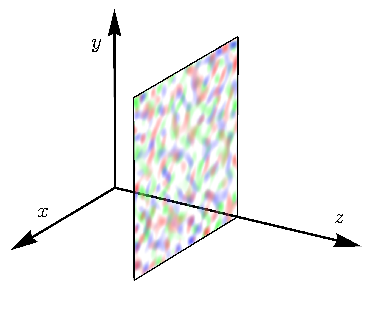
\includegraphics[width=0.9\textwidth]{images/sheets1.pdf}
        \end{figure}
       \column{.033\textwidth}
       \column{.5\textwidth}
       \vspace{-5pt}
        \begin{custombox2}{MV model}{lightgray}
            \small
            \begin{varwidth}{0.96\textwidth}
            \begin{itemize}\itemsep0em 
                \setbeamertemplate{itemize item}{\raisebox{0.2em}{\scalebox{0.7}{${\color{palteal}\blacktriangleright}$}}} 
                \item {\color{palteal}\bfseries Color current} of nucleus $\rightarrow$ generated by \\{\color{palgold}\bfseries color charge} $\color{palgold}\boldsymbol{\rho}$ $\leftrightarrow$ stochastic variable
            \end{itemize}
            \end{varwidth}
        \end{custombox2}

        % \begin{itemize}\itemsep0em 
        %     \footnotesize\color{lightgray}
        %     \setbeamertemplate{itemize item}{\raisebox{0.2em}{\scalebox{0.6}{${\color{lightgray}\blacktriangleright}$}}}
        %     \item {\color{palteal}Color current} of nucleus $\rightarrow$ generated\\ by {\color{palgold} color charge} density
        % \end{itemize}
        \begin{itemize}\itemsep0em 
            \setbeamertemplate{itemize item}{\raisebox{0.2em}{\scalebox{0.7}{${\color{palgold}\blacktriangleright}$}}}
            \item {\bfseries\color{palgold} MV model} for color charges ${\color{palgold}\boldsymbol{\rho}}$
        \end{itemize}
        \vspace{5pt}
        \renewcommand{\eqnhighlightheight}{\vphantom{\mathcal{D}_\mu}\mathstrut}\begin{equation*}
            \big\langle{\color{palgold}\boldsymbol{\rho}}(\vec{x}_\perp){\color{palgold}\boldsymbol{\rho}}(\vec{y}_\perp)\big\rangle\propto\hspace{-3pt}\eqnmark[normal]{g2mu}{{\color{palviolet}\boldsymbol{g^2\mu}}}\hspace{-3pt}^2\delta^{(2)}(\vec{x}_\perp-\vec{y}_\perp)
            \end{equation*}
            \annotate[yshift=-0.7em]{below, right}{g2mu}{\scriptsize ${\color{palviolet}\boldsymbol{g^2\mu}}\propto{\color{palviolet}\boldsymbol{Q_s}}$}
            \vspace{5pt}
            \begin{itemize}\itemsep0em 
                \setbeamertemplate{itemize item}{\raisebox{0.2em}{\scalebox{0.7}{${\color{palviolet}\blacktriangleright}$}}}
                \item {\color{palviolet}\bfseries Saturation momentum $\boldsymbol{Q_s}$} \\{\scriptsize\color{lightgray} $Q_s\approx 2\,\mathrm{GeV}$ at LHC central collisions}
            \end{itemize}    
        \begin{itemize}\itemsep0em 
            \setbeamertemplate{itemize item}{\raisebox{0.2em}{\scalebox{0.7}{${\color{jyured}\blacktriangleright}$}}}
            \item {\bfseries\color{jyured}Glasma improvements}: {\bfseries\color{palgold} proton/nuclear structure} by modelling ${\color{palgold}\boldsymbol{\rho}}(\vec{x}_\perp)$ 
        \end{itemize}      
        \column{.033\textwidth}
    \end{columns}
    \blfootnote{\scriptsize McLerran, Venugopalan \href{https://arxiv.org/abs/hep-ph/9309289}{{\color{palgold}\texttt{[hep-ph/9309289]}$^\text{\scalebox{0.9}{\faExternalLink}}$}} Müller \href{https://arxiv.org/abs/1904.04267}{{\color{palviolet}\texttt{[1904.04267]}$^\text{\scalebox{0.9}{\faExternalLink}}$}}}
\end{frame}


%%%%%%%%%%%%%%%%%%%%%%%%%%%%%%%%%%%%%%%%%
%%%%%%%%%%%%%%%%% SLIDE %%%%%%%%%%%%%%%%%
%%%%%%%%%%%%%%%%%%%%%%%%%%%%%%%%%%%%%%%%%

\begin{frame}
    \frametitle{Collision of CGC fields}
    \framesubtitle{How to obtain the glasma fields}
    \vspace{-5pt}
    \begin{columns}[onlytextwidth,t]
        \column{.033\textwidth}
        \column{.4\textwidth}

        \begin{itemize}\itemsep0em 
            \item Light-cone diagram of collision\\
            {\scriptsize\color{lightgray} Light-cone coordinates $x^\pm=t\pm z$}
        \end{itemize}
        \begin{tikzpicture}[]
            \node[anchor=south west,inner sep=0] at (0,0) {\includegraphics[width=\textwidth]{images/spacetb.eps}};
            \node[isosceles triangle,
                isosceles triangle apex angle=90,
                draw=palviolet,opacity=0.05,
                fill=palviolet,fill opacity=0.1,
                minimum size =2cm] (T90)at (1.8,2.2){};
            \node[isosceles triangle,
                isosceles triangle apex angle=90,
                draw=palviolet,opacity=0.05,
                fill=palviolet,fill opacity=0.1,
                rotate=180,
                minimum size =2cm] (T90)at (4.25,2.2){};
            \node[isosceles triangle,
                isosceles triangle apex angle=90,
                draw=palgold,opacity=0.05,line width=1pt,
                fill=palgold,fill opacity=0.1,
                rotate=270,
                minimum size =2cm] (T90)at (3.03,3.43){};
        \end{tikzpicture}

       \column{.05\textwidth}
       \column{.5\textwidth}
        \begin{custombox2}{{\normalsize CGC fields} {\tiny (regions 1, 2)}}{palviolet}
            \small
            \begin{varwidth}{0.93\textwidth}
            \begin{itemize}\itemsep0em 
                \setbeamertemplate{itemize item}{\raisebox{0.2em}{\scalebox{0.7}{${\color{palviolet}\blacktriangleright}$}}} 
                \footnotesize
                \item Analytical {\color{red}\bfseries pure gauge} fields before collision
                % \item Weizsäcker–Williams gluon distribution
            \end{itemize}
            \end{varwidth}
        \end{custombox2}

        \begin{custombox2}{{\normalsize Initial condition} {\tiny (along light-cone)}}{normal}
            \small
            \begin{varwidth}{0.93\textwidth}
            \begin{itemize}\itemsep0em 
                \setbeamertemplate{itemize item}{\raisebox{0.2em}{\scalebox{0.7}{${\color{normal}\blacktriangleright}$}}} 
                \footnotesize
                \item Match CGC fields on the light cone
                \item Impose {\bfseries boost-invariance} $\Rightarrow$ 2+1D fields\\
                {\tiny\color{lightgray} Milne coordinates {\color{Blue}$\tau=\sqrt{x^+x^-}$} and {\color{ForestGreen}$\eta=\mathrm{ln}(x^+/x^-)$}}
                \setbeamertemplate{itemize item}{\raisebox{0.2em}{\scalebox{0.7}{${\color{jyured}\blacktriangleright}$}}} 
                \footnotesize
                \item {\bfseries\color{jyured}Glasma improvements}: 3+1D fields
            \end{itemize}
            \end{varwidth}
        \end{custombox2}

        \begin{custombox2}{{\normalsize Glasma fields} {\tiny (region 3)}}{palgold}
            \small
            \begin{varwidth}{0.93\textwidth}
            \begin{itemize}\itemsep0em 
                \setbeamertemplate{itemize item}{\raisebox{0.2em}{\scalebox{0.7}{${\color{palgold}\blacktriangleright}$}}} 
                \footnotesize
                \item Numerically solve CYM equations on lattice
                \item Real-time lattice gauge theory techniques \\
                {\tiny\color{lightgray} Discretize with gauge links and plaquette variables}
            \end{itemize}
            \end{varwidth}
        \end{custombox2}
        \column{.033\textwidth}
    \end{columns}
    \blfootnote{\scriptsize Lappi \href{https://arxiv.org/abs/hep-ph/0602189}{{\color{palgold}\texttt{[hep-ph/0602189]}$^\text{\scalebox{0.9}{\faExternalLink}}$}}}
    \begin{tikzpicture}[overlay, remember picture]
        \node[anchor=north west] 
        at ([xshift=0.05cm,yshift=-0.05cm]current page.north west) {\begin{talkbox}\scriptsize{\color{destacado}Mrowczynski$\hspace{1pt}^\text{\scalebox{0.9}{\faComment}}$} {\itshape Tue 9:00$\hspace{1pt}^\text{\scalebox{0.9}{\faClockO}}$} \end{talkbox}};
    \end{tikzpicture}
    \begin{tikzpicture}[overlay, remember picture]
        \node[anchor=north west] 
        at ([xshift=0.05cm,yshift=-0.48cm]current page.north west) {\begin{talkbox}\scriptsize{Glasma in $\tau$ expansion} \end{talkbox}};
    \end{tikzpicture}
    \begin{tikzpicture}[overlay, remember picture]
        \node[anchor=north west] 
        at ([xshift=0.05cm,yshift=-1.05cm]current page.north west) {\begin{talkbox}\scriptsize{\color{destacado}Ipp$\hspace{1pt}^\text{\scalebox{0.9}{\faComment}}$} {\itshape Tue 14:30$\hspace{1pt}^\text{\scalebox{0.9}{\faClockO}}$} \end{talkbox}};
    \end{tikzpicture}
    \begin{tikzpicture}[overlay, remember picture]
        \node[anchor=north west] 
        at ([xshift=0.05cm,yshift=-1.48cm]current page.north west) {\begin{talkbox}\scriptsize{3+1D glasma} \end{talkbox}};
    \end{tikzpicture}
\end{frame}


%%%%%%%%%%%%%%%%%%%%%%%%%%%%%%%%%%%%%%%%%
%%%%%%%%%%%%%% SUBSECTION %%%%%%%%%%%%%%%
%%%%%%%%%%%%%%%%%%%%%%%%%%%%%%%%%%%%%%%%%

\subsection{Features}

%%%%%%%%%%%%%%%%%%%%%%%%%%%%%%%%%%%%%%%%%
%%%%%%%%%%%%%%%%% SLIDE %%%%%%%%%%%%%%%%%
%%%%%%%%%%%%%%%%%%%%%%%%%%%%%%%%%%%%%%%%%

\begin{frame}
    \frametitle{Features of the glasma}
    \begin{itemize}\itemsep0em 
        \setbeamertemplate{itemize item}{\raisebox{0.2em}{\scalebox{0.7}{${\color{destacado}\blacktriangleright}$}}} 
        \item \begin{center}Physics of glasma determined by the {\bfseries saturation momentum} $\boldsymbol{Q_s}$\end{center}
    \end{itemize}
    \vspace{-10pt}
    \begin{columns}[onlytextwidth,t]
        \column{.025\textwidth}
        \column{.3\textwidth}

        \begin{custombox2}{{\normalsize Flux tubes}}{palteal}
            \begin{varwidth}{0.99\columnwidth}
            \begin{itemize}\itemsep0em 
                \setbeamertemplate{itemize item}{\raisebox{0.2em}{\scalebox{0.7}{${\color{palteal}\blacktriangleright}$}}} 
                \scriptsize
                \item Initially only longitudinal electric and magnetic fields
            \end{itemize}
            \end{varwidth}
        \end{custombox2}

       \column{.025\textwidth}
       \column{.3\textwidth}
       \begin{custombox2}{{\normalsize Strong fields}}{palviolet}
            \begin{varwidth}{0.95\columnwidth}
            \begin{itemize}\itemsep0em 
                \setbeamertemplate{itemize item}{\raisebox{0.2em}{\scalebox{0.7}{${\color{palviolet}\blacktriangleright}$}}} 
                \scriptsize
                \item Strong longitudinal fields dilute after $\tau\sim 1/\boldsymbol{Q_s}$
            \end{itemize}
            \end{varwidth}
        \end{custombox2}

        \column{.025\textwidth}
        \column{.3\textwidth}
        \begin{custombox2}{{\normalsize Correlation domains}}{palgold}
            \begin{varwidth}{0.99\columnwidth}
            \begin{itemize}\itemsep0em 
                \setbeamertemplate{itemize item}{\raisebox{0.2em}{\scalebox{0.7}{${\color{palgold}\blacktriangleright}$}}} 
                \scriptsize
                \item Fields correlated inside\\ flux tubes of size $\sim 1/\boldsymbol{Q_s}$ 
            \end{itemize}
            \end{varwidth}
        \end{custombox2}
 
        \column{.025\textwidth}
    \end{columns}

    \begin{columns}[onlytextwidth,t]
        \column{.3\textwidth}

        \vspace{5pt}
        \begin{center}
            \begin{figure}
                \centering
                \hspace{-5pt}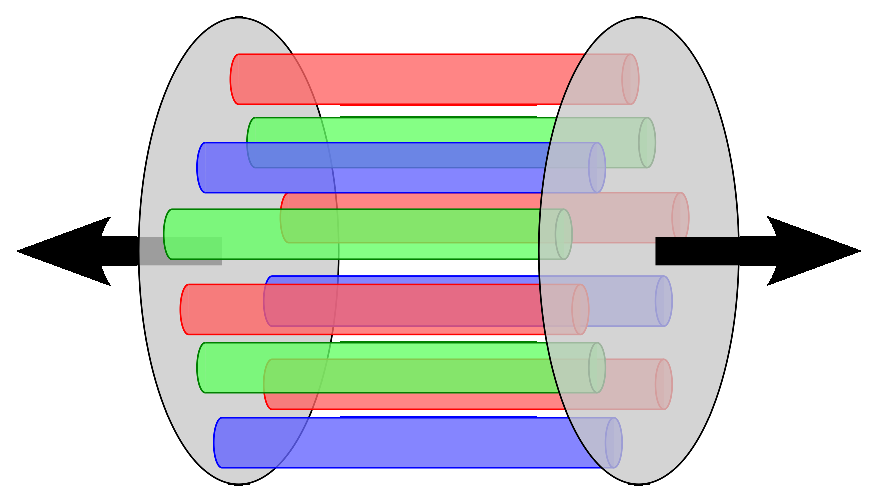
\includegraphics[width=0.9\textwidth]{images/glasma.eps}
            \end{figure}
        \end{center}

       \column{.025\textwidth}
       \column{.3\textwidth}
        \begin{center}
            \begin{figure}
                \centering
                \hspace{-5pt}\includegraphics[width=0.9\textwidth]{images/components.eps}
            \end{figure}
        \end{center}

        \column{.025\textwidth}
        \column{.3\textwidth}
        \begin{center}
            \begin{figure}
                \centering
                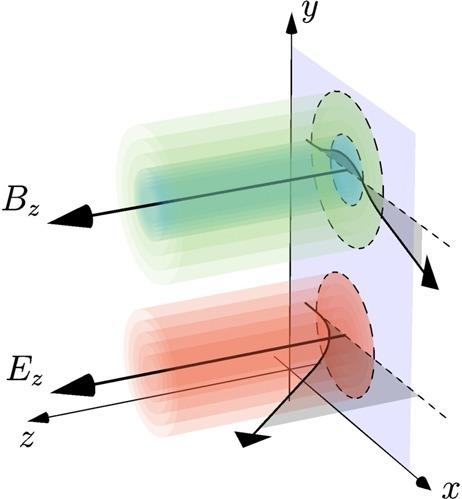
\includegraphics[width=0.7\textwidth]{images/1-s2.0-S0370269320306134-gr003_lrg.jpg}
            \end{figure}
        \end{center}

        \column{.05\textwidth}
    \end{columns}
    \blfootnote{\scriptsize Fukushima \href{https://arxiv.org/abs/1603.02340}{{\color{palteal}\texttt{[1603.02340]}$^\text{\scalebox{0.9}{\faExternalLink}}$}} Lappi \href{https://arxiv.org/abs/hep-ph/0606207}{{\color{palviolet}\texttt{[hep-ph/0606207]}$^\text{\scalebox{0.9}{\faExternalLink}}$}} Ipp, Müller, Schuh \href{https://arxiv.org/abs/2009.14206}{{\color{palgold}\texttt{[2009.14206]}$^\text{\scalebox{0.9}{\faExternalLink}}$}}
    }
    \begin{tikzpicture}[overlay, remember picture]
        \node[anchor=north west] 
        at ([xshift=0.05cm,yshift=-0.05cm]current page.north west) {\begin{talkbox}\scriptsize{\color{destacado}Ruggieri$\hspace{1pt}^\text{\scalebox{0.9}{\faComment}}$} {\itshape Mon 11:00$\hspace{1pt}^\text{\scalebox{0.9}{\faClockO}}$} \end{talkbox}};
    \end{tikzpicture}
    \begin{tikzpicture}[overlay, remember picture]
        \node[anchor=north west] 
        at ([xshift=0.05cm,yshift=-0.48cm]current page.north west) {\begin{talkbox}\scriptsize{Glasma properties} \end{talkbox}};
    \end{tikzpicture}
\end{frame}


\begin{frame}
    \frametitle{Features of the glasma}
    \framesubtitle{Energy density profiles}
    \begin{figure}
        \centering
        \includegraphics[width=0.9\textwidth]{images/flux_tubes_auau_200_nums_1_dpi_300_nounits.png}
        \captionsetup{justification=centering}
        \caption{Relevant scale ${\color{custompink}\boldsymbol{Q_s}}$ \\
        {\scriptsize Fields arrange themselves in \textit{\textbf{\color{customgreen} correlation domains}} of $\delta x_T \simeq {\color{custompink}\boldsymbol{Q}}^{-1}_{\color{custompink}\boldsymbol{s}}$, \textit{\textbf{\color{customgreen} dilute}} after $\delta\tau\simeq {\color{custompink}\boldsymbol{Q}}^{-1}_{\color{custompink}\boldsymbol{s}}$, } 
        }
    \end{figure}
\end{frame}

\begin{frame}[noframenumbering]
    \frametitle{Features of the glasma}
    \framesubtitle{Correlation domains}
    {\transparent{0.05}\begin{figure}
        \centering
        \includegraphics[width=0.9\textwidth]{images/flux_tubes_auau_200_nums_1_dpi_300_nounits.png}
        \captionsetup{justification=centering}
        \caption{Relevant scale ${\color{custompink}Q_s}$ \\
        {\scriptsize\itshape Fields {\color{customgreen}dilute} after $\delta\tau\simeq {\color{custompink}Q}^{-1}_{\color{custompink}s}$, arrange themselves in {\color{customgreen}\bfseries correlation domains} of $\delta x_T \simeq {\color{custompink}\boldsymbol{Q}}^{-1}_{\color{custompink}\boldsymbol{s}}$} 
        }
    \end{figure}}
    \vspace{0.3cm}
    \begin{center}
        \begin{tikzpicture}[remember picture,overlay]
            \node[align=center] at (0,4) {
                The fields arrange themselves in {\color{customgreen}\bfseries correlation domains} of $\delta x_T \simeq {\color{custompink}\boldsymbol{Q}}^{-1}_{\color{custompink}\boldsymbol{s}}$\\[-5pt]
                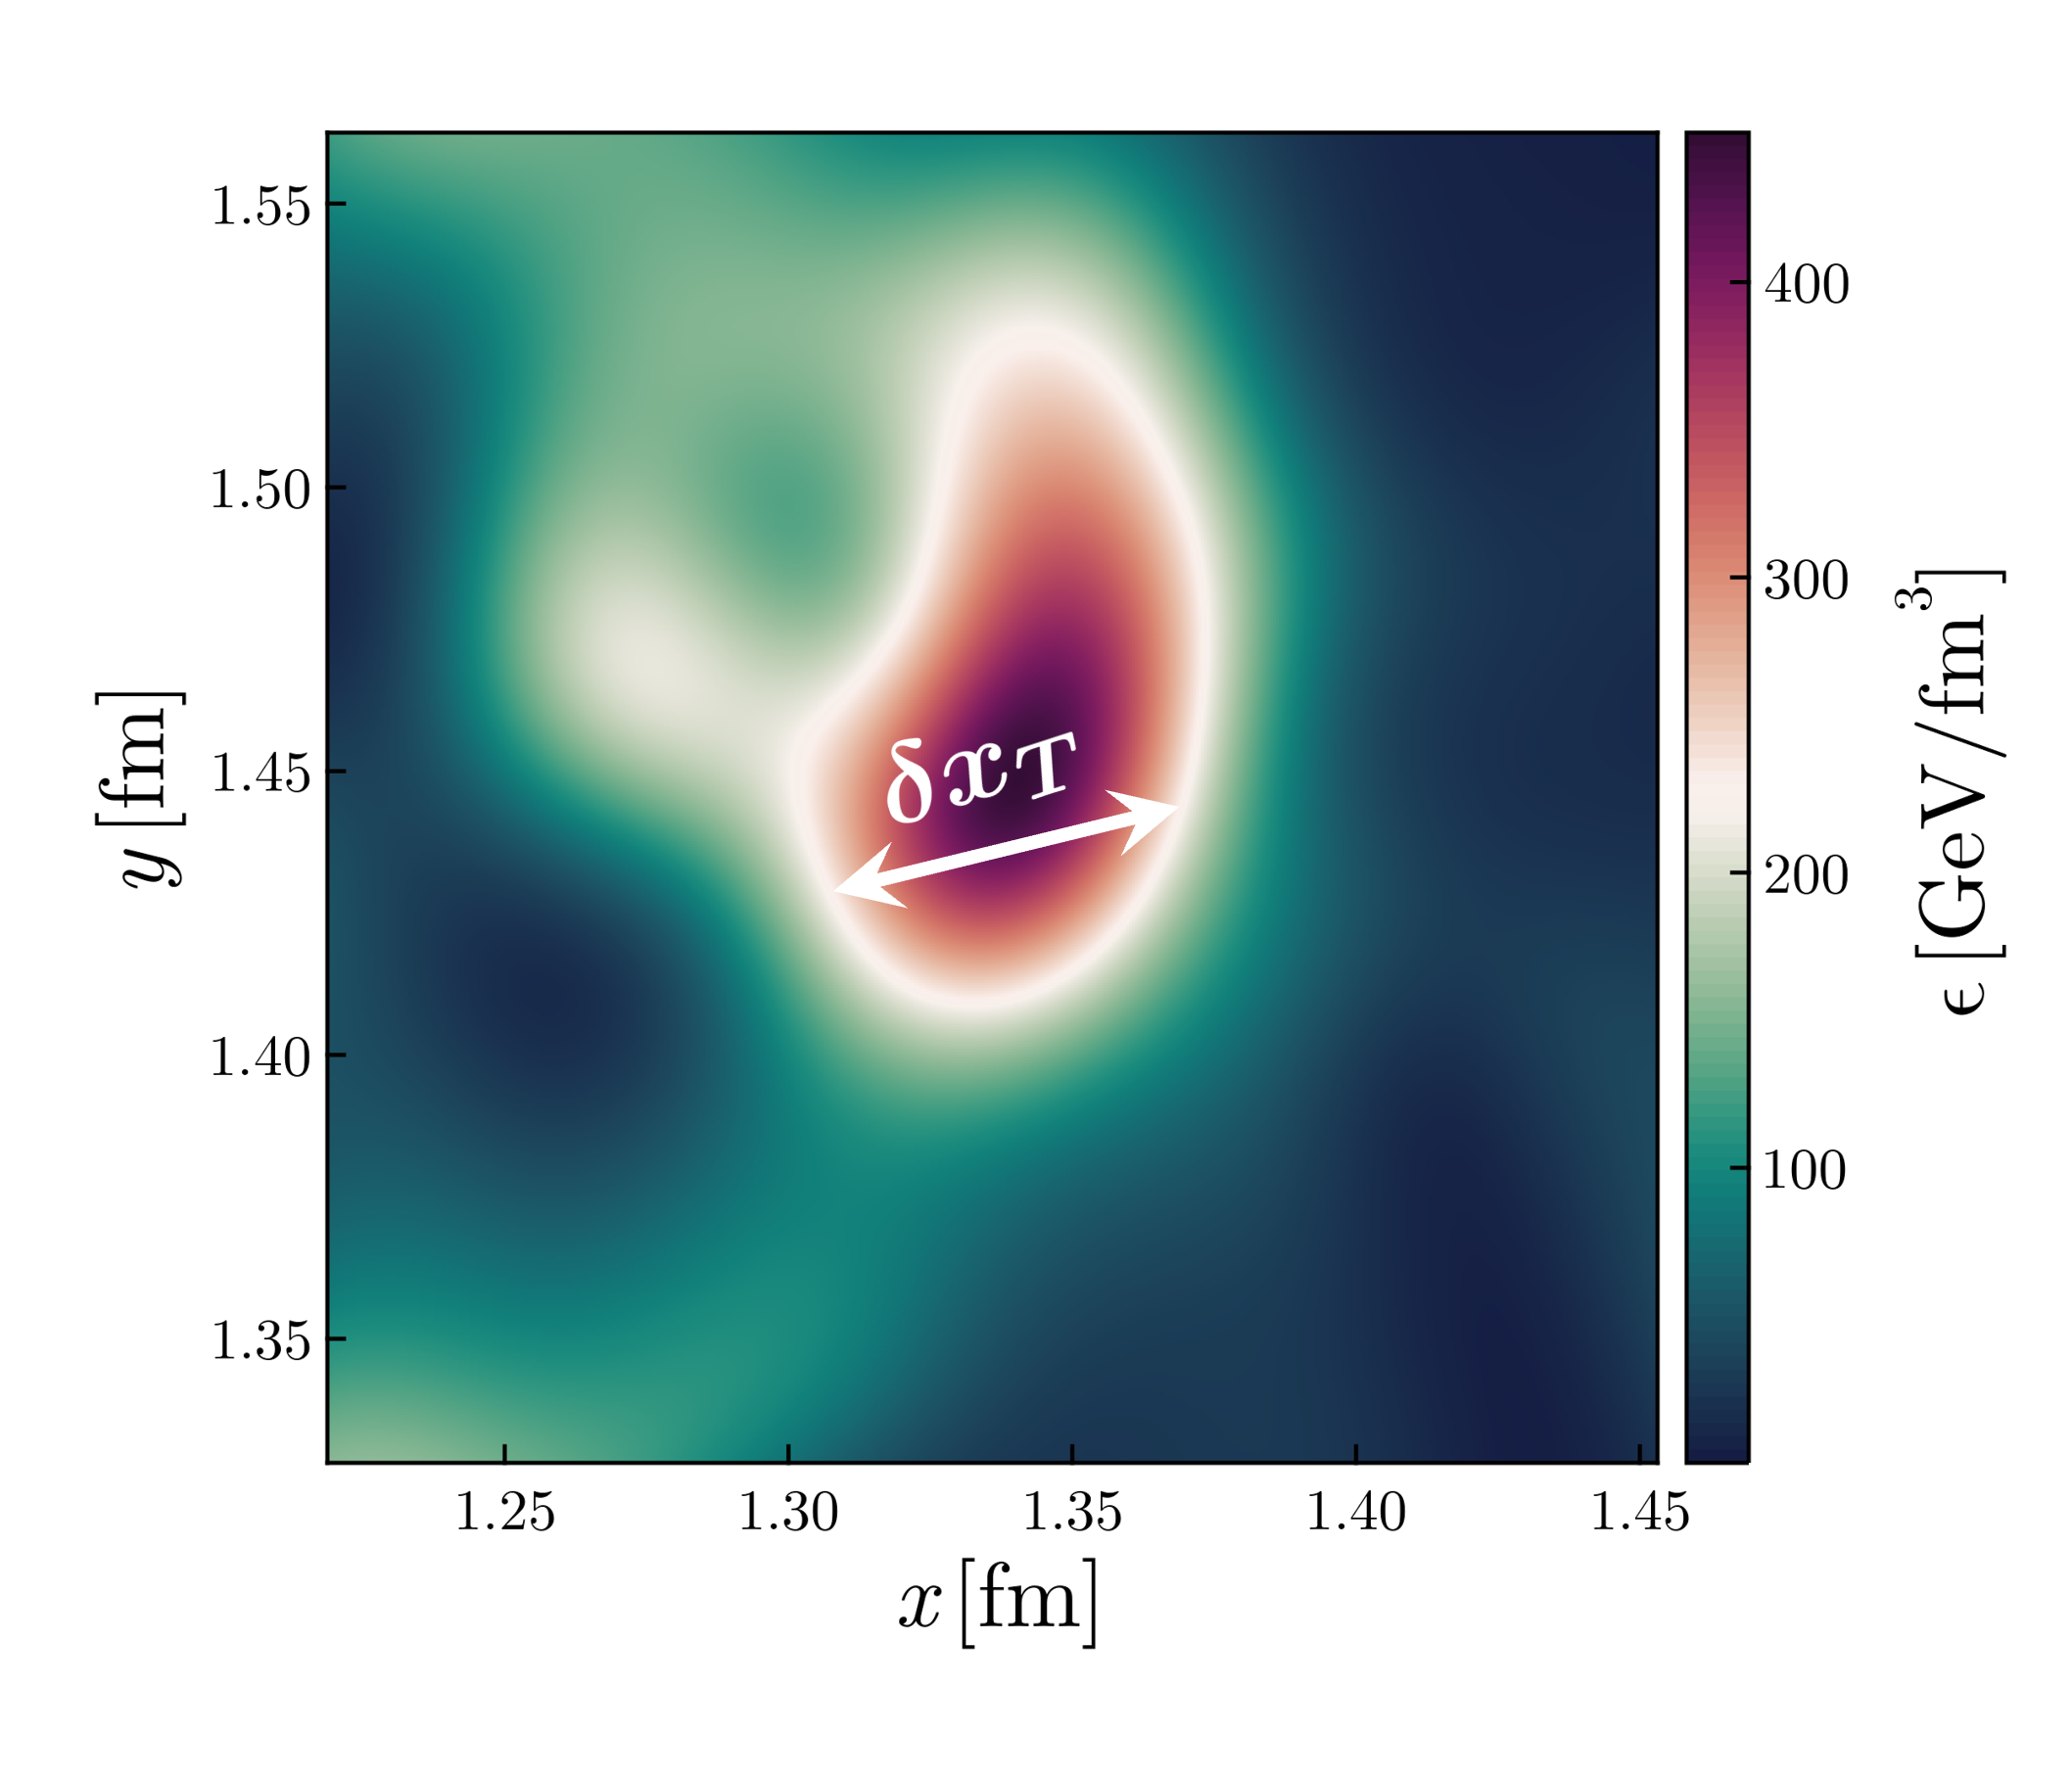
\includegraphics[width=0.48\textwidth]{images/correlation_2.png}
            };
        \end{tikzpicture} 
    \end{center}
\end{frame}

\begin{frame}[noframenumbering]
    \frametitle{Features of the glasma}
    \framesubtitle{Bjorken expansion}
    {\transparent{0.05}\begin{figure}
        \centering
        \includegraphics[width=0.9\textwidth]{images/flux_tubes_auau_200_nums_1_dpi_300_nounits.png}
        \captionsetup{justification=centering}
        \caption{Relevant scale ${\color{custompink}Q_s}$ \\
        {\scriptsize\itshape Fields {\color{customgreen}\bfseries dilute} after $\delta\tau\simeq {\color{custompink}Q}^{-1}_{\color{custompink}s}$, arrange themselves in {\color{customgreen}correlation domains} of $\delta x_T \simeq {\color{custompink}\boldsymbol{Q}}^{-1}_{\color{custompink}\boldsymbol{s}}$} 
        }
    \end{figure}}
    \begin{center}
        \begin{tikzpicture}[remember picture,overlay]
            \node[align=center] at (0,4) {
                The fields become {\color{customgreen}\bfseries dilute} after $\delta\tau\simeq {\color{custompink}\boldsymbol{Q}}^{-1}_{\color{custompink}\boldsymbol{s}}$\\
                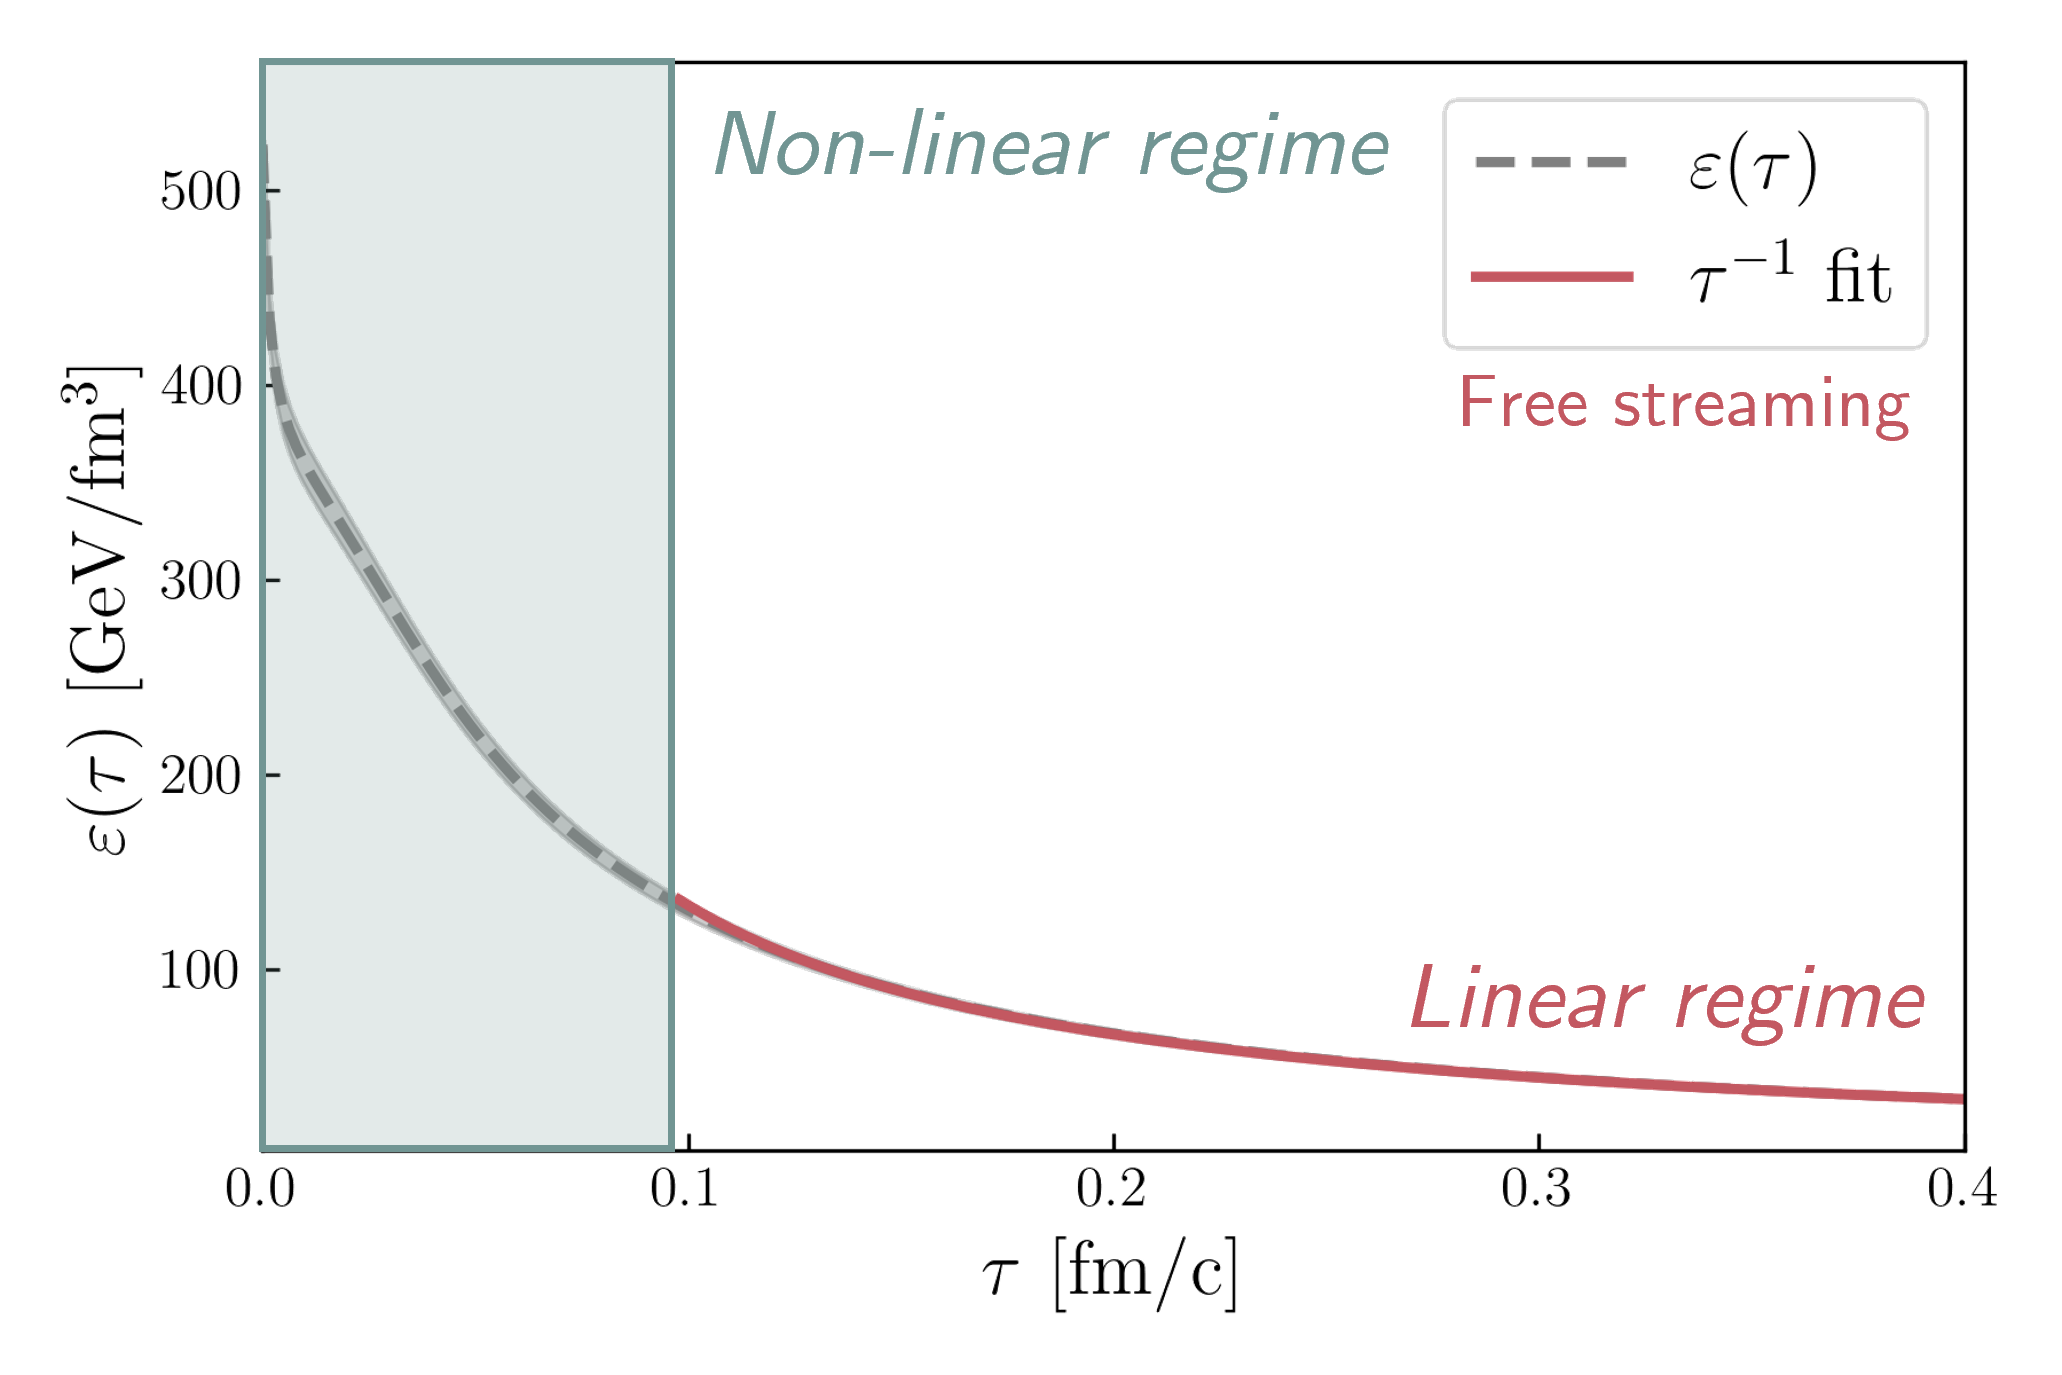
\includegraphics[width=0.55\textwidth]{images/dilute_2.png}
            };
        \end{tikzpicture} 
    \end{center}
\end{frame}



\begin{frame}[noframenumbering]
    \frametitle{Features of the glasma}
    \framesubtitle{Anisotropic fields}
    {\transparent{0.05}\begin{figure}
        \centering
        \includegraphics[width=0.9\textwidth]{images/flux_tubes_auau_200_nums_1_dpi_300_nounits.png}
        \captionsetup{justification=centering}
        \caption{Relevant scale ${\color{custompink}Q_s}$ \\
        {\scriptsize\itshape Fields {\color{customgreen}dilute} after $\delta\tau\simeq {\color{custompink}Q}^{-1}_{\color{custompink}s}$, arrange themselves in {\color{customgreen}correlation domains} of $\delta x_T \simeq {\color{custompink}Q}^{-1}_{\color{custompink}s}$} 
        }
    \end{figure}}
    \vspace{0.3cm}
    \begin{center}
        \begin{tikzpicture}[remember picture,overlay]
            \node[align=center] at (0,4) {
                Longitudinal $\neq$ transverse $\Rightarrow$ {\color{pinky}\bfseries anisotropy}\\
                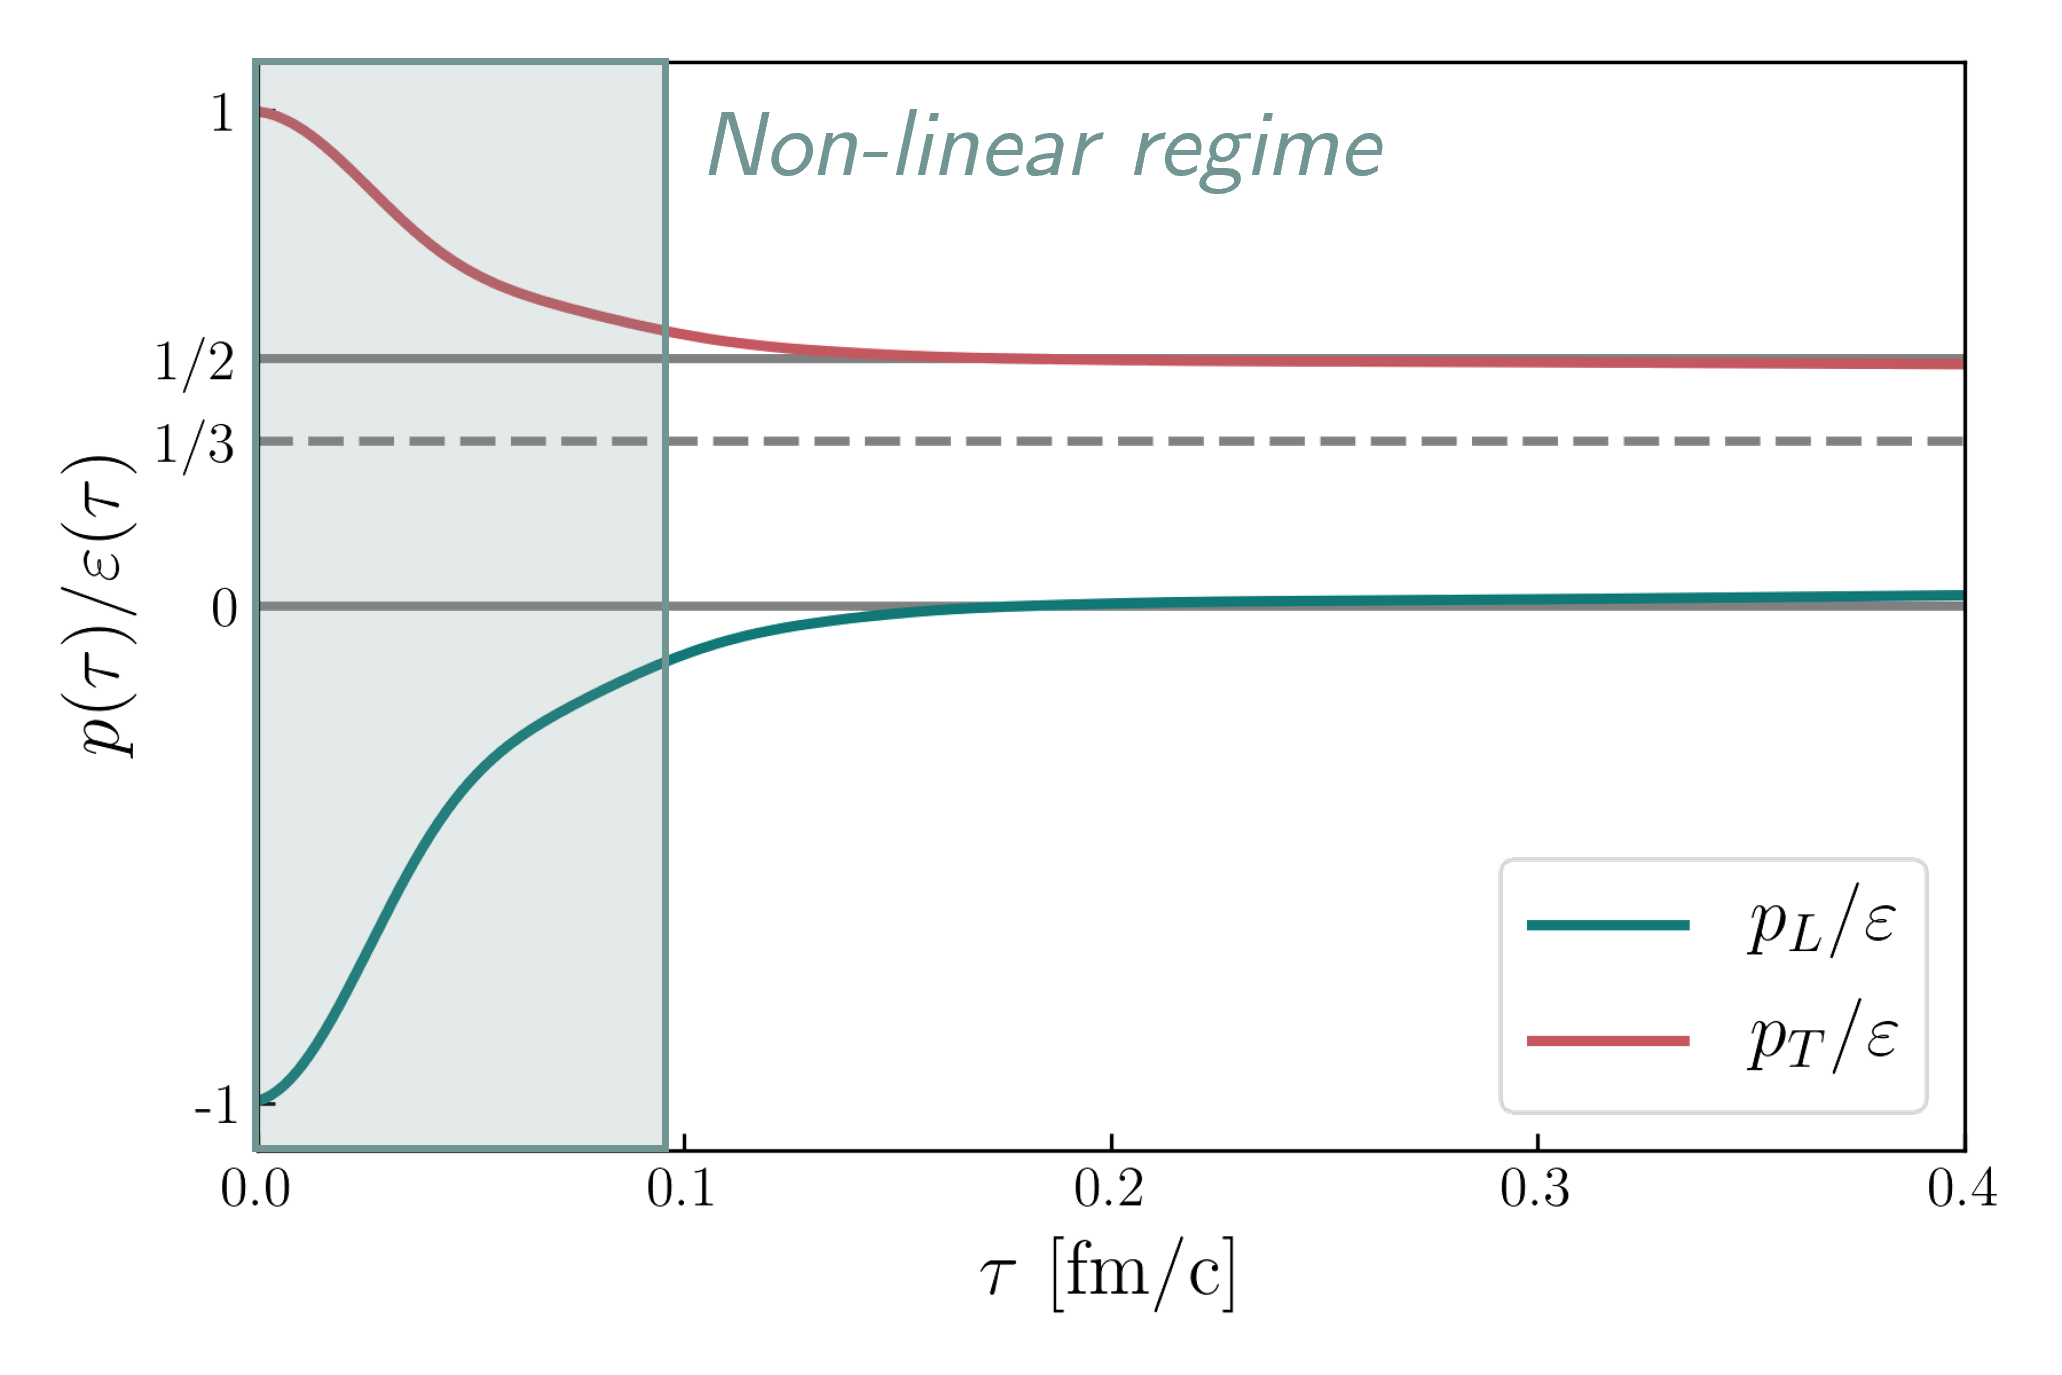
\includegraphics[width=0.55\textwidth]{images/anisotropy.png}
            };
        \end{tikzpicture} 
    \end{center}
\end{frame}


%%%%%%%%%%%%%%%%%%%%%%%%%%%%%%%%%%%%%%%%%
%%%%%%%%%%%%%%%% SECTION %%%%%%%%%%%%%%%%
%%%%%%%%%%%%%%%%%%%%%%%%%%%%%%%%%%%%%%%%%

\section{Transport in glasma}


%%%%%%%%%%%%%%%%%%%%%%%%%%%%%%%%%%%%%%%%%
%%%%%%%%%%%%%%%%% SLIDE %%%%%%%%%%%%%%%%%
%%%%%%%%%%%%%%%%%%%%%%%%%%%%%%%%%%%%%%%%%

\setbeamertemplate{background}{
\tikz[overlay,remember picture] \node[opacity=0.1, at=(current page.center), align=center] {\\[10pt]
{\transparent{0.1}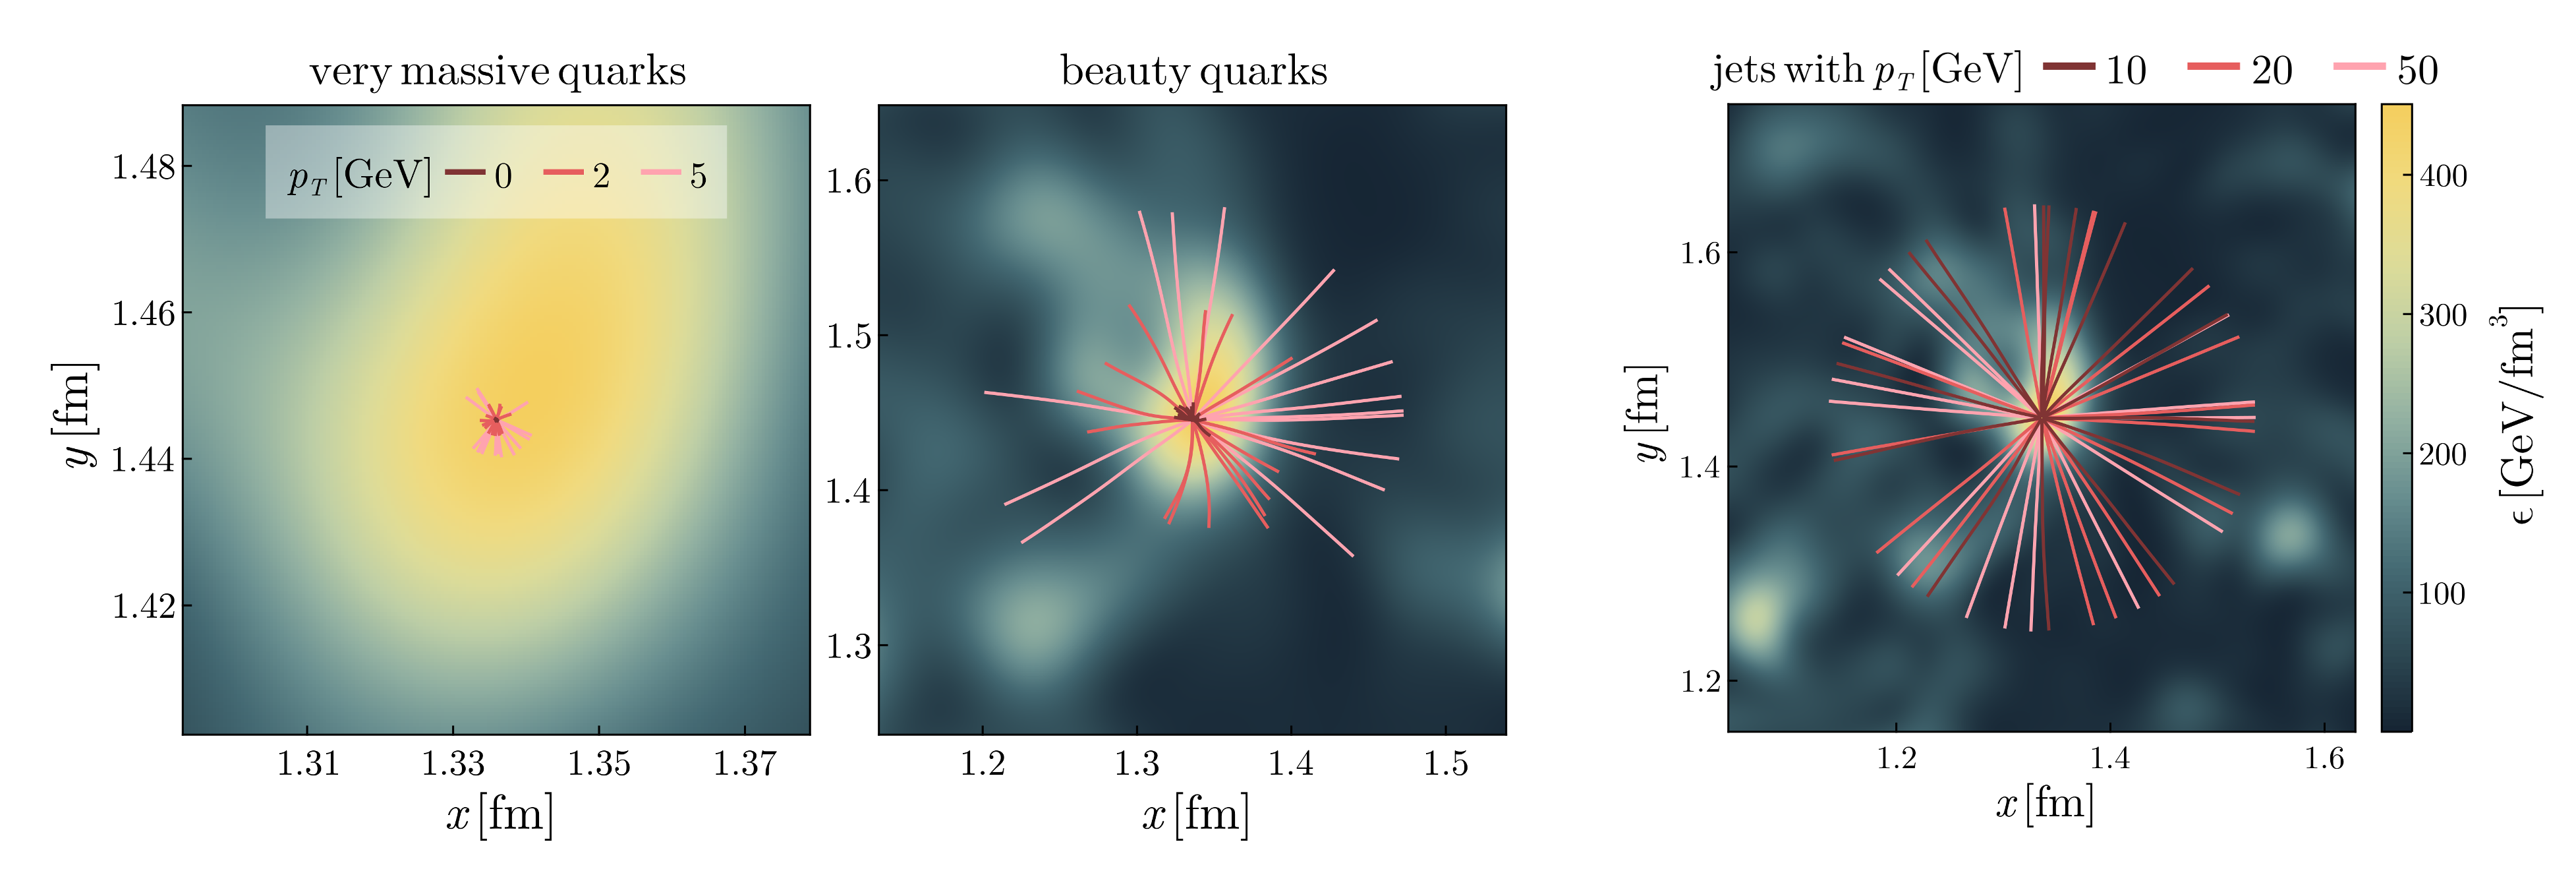
\includegraphics[width=\paperwidth]{images/hqs_jets_trajectories.png}}};
}
\setbeamertemplate{itemize item}{\raisebox{0.2em}{\scalebox{0.7}{${\color{normal}\blacktriangleright}$}}} 
\begin{frame}[plain,noframenumbering]{}
    \begin{center}
        \vspace{1cm}
        {\large\color{normal}Transport during pre-equilibrium}\\[0.3cm]
        {\huge\color{destacado}Hard probes in glasma}\\[0.3cm]
    \end{center}
\end{frame}
\setbeamertemplate{background}{}

%%%%%%%%%%%%%%%%%%%%%%%%%%%%%%%%%%%%%%%%%
%%%%%%%%%%%%%%%%% SLIDE %%%%%%%%%%%%%%%%%
%%%%%%%%%%%%%%%%%%%%%%%%%%%%%%%%%%%%%%%%%

\setbeamertemplate{background}{
\tikz[overlay,remember picture] \node[at=(current page.center), align=center] {\\[20pt]
{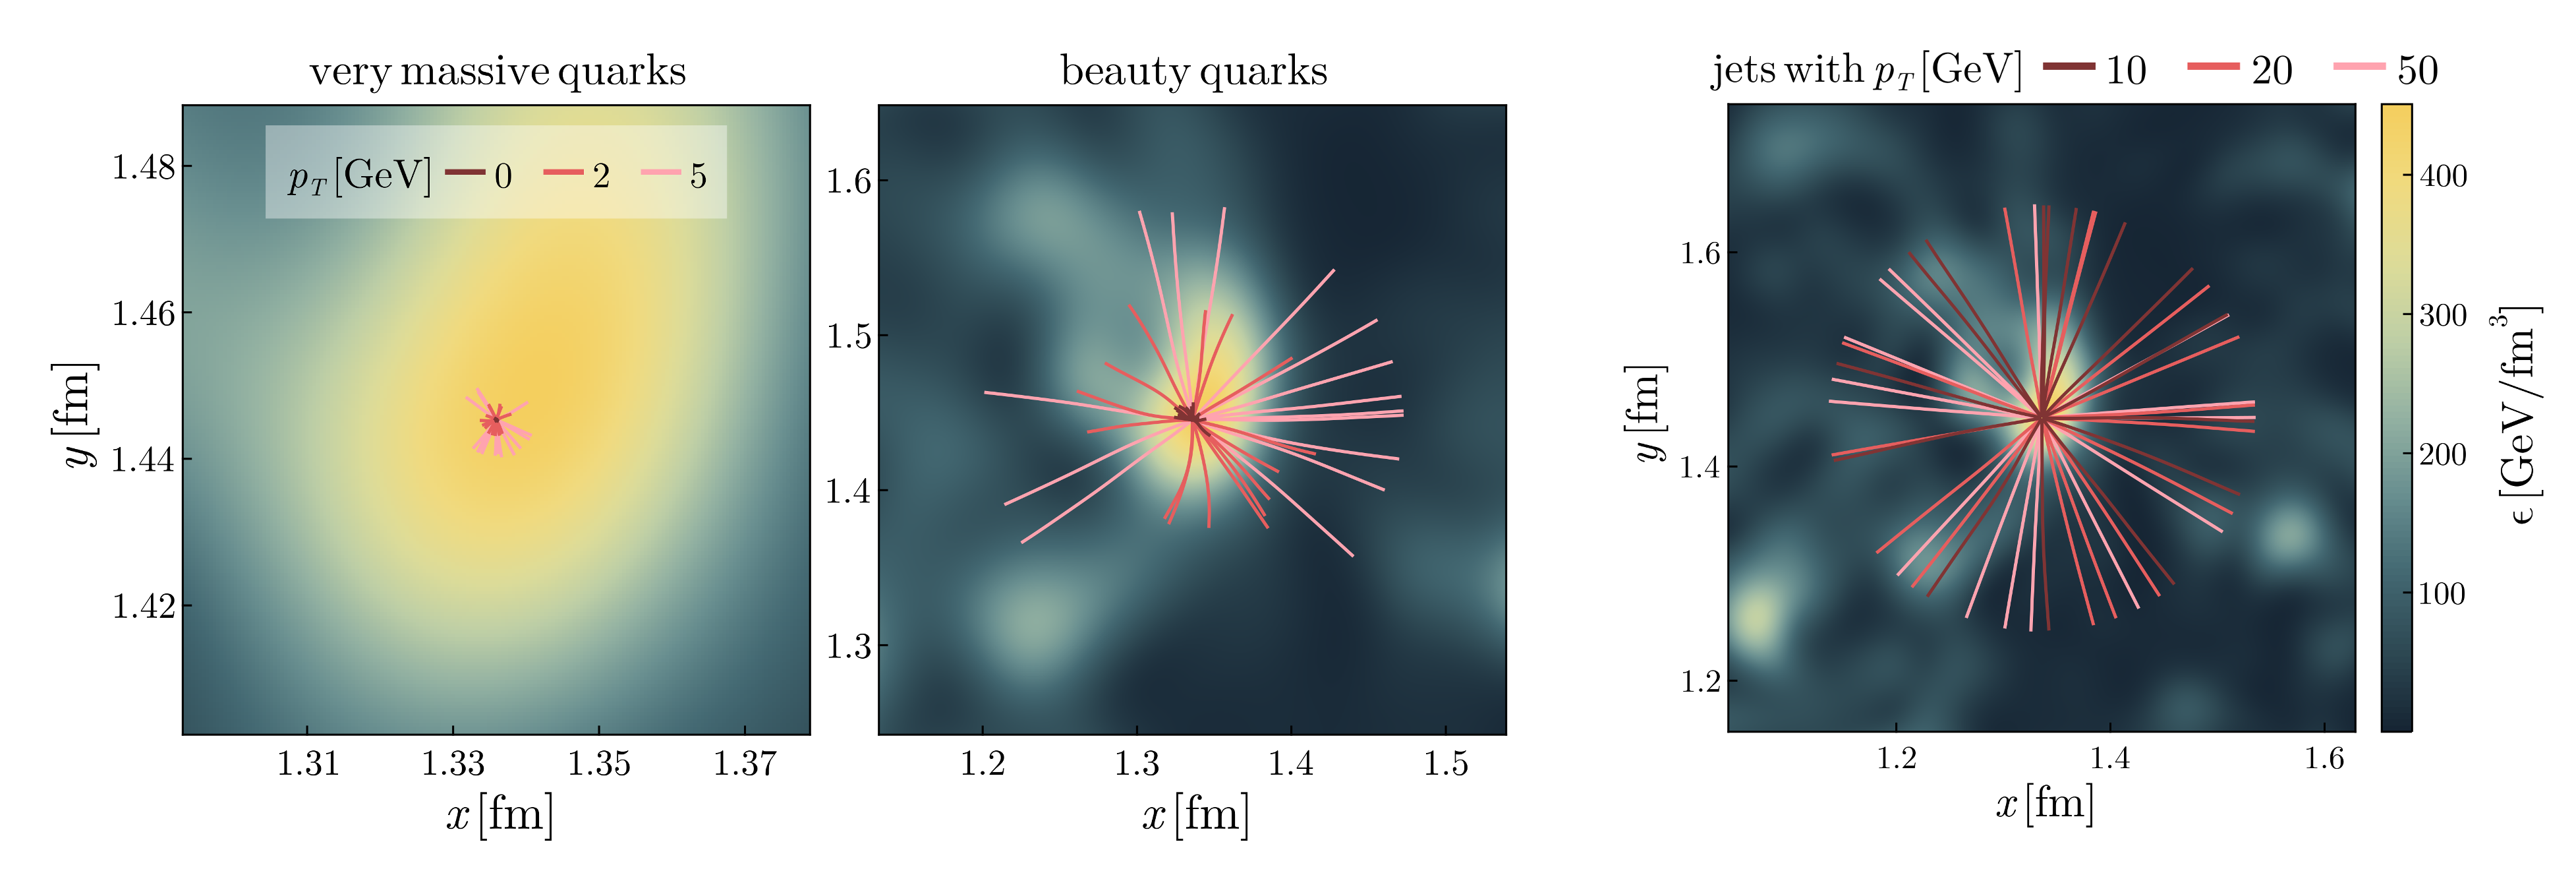
\includegraphics[width=\paperwidth]{images/hqs_jets_trajectories.png}}};
}
\setbeamertemplate{itemize item}{\raisebox{0.2em}{\scalebox{0.7}{${\color{normal}\blacktriangleright}$}}} 
\begin{frame}[plain, noframenumbering]
    \frametitle{\\ Heavy quarks and jets in glasma}
    \framesubtitle{Probing the glasma fields}
    \blfootnote{\scriptsize DA, Băran, Greco, Ipp, Müller, Ruggieri  \href{https://arxiv.org/abs/2303.05599}{{\color{palgold}\texttt{[2303.05599]}$^\text{\scalebox{0.9}{\faExternalLink}}$}}}
\end{frame}
\setbeamertemplate{background}{}


%%%%%%%%%%%%%%%%%%%%%%%%%%%%%%%%%%%%%%%%%
%%%%%%%%%%%%%% SUBSECTION %%%%%%%%%%%%%%%
%%%%%%%%%%%%%%%%%%%%%%%%%%%%%%%%%%%%%%%%%

\subsection{Classical transport}

%%%%%%%%%%%%%%%%%%%%%%%%%%%%%%%%%%%%%%%%%
%%%%%%%%%%%%%%%%% SLIDE %%%%%%%%%%%%%%%%%
%%%%%%%%%%%%%%%%%%%%%%%%%%%%%%%%%%%%%%%%%

\begin{frame}
    \frametitle{Particles in Yang-Mills fields}
    \framesubtitle{Wong's equations of motion}
        \setbeamertemplate{itemize item}{\raisebox{0.2em}{\scalebox{0.7}{${\color{ming}\blacktriangleright}$}}} 
   \begin{center}
    \begin{custombox2}{Classical transport equations}{lightgray}
        \small
        \begin{varwidth}{0.68\textwidth}
        \begin{itemize}\itemsep0em 
            \setbeamertemplate{itemize item}{\raisebox{0.2em}{\scalebox{0.7}{${\color{lightgray}\blacktriangleright}$}}} 
            \item Wong's equations $\leftrightarrow$ classical equations of motion for particles\\
            $({\color{customblue}x^\mu},{\color{customred}p^\mu},{\color{customyellow}Q})$ evolving in a Yang-Mills background field ${\color{starrysecond}A^\mu}$
        \end{itemize}
        \end{varwidth}
    \end{custombox2}

    %    Wong's equations $\leftrightarrow$ classical equations of motion for particles $({\color{customblue}x^\mu},{\color{customred}p^\mu},{\color{customyellow}Q})$ \\
    % evolving in a Yang-Mills background field ${\color{starrysecond}A^\mu}$
   \end{center} 
        \vspace{1cm}
        \renewcommand{\eqnhighlightheight}{\vphantom{x}}
        \begin{equation*}
            \frac{\d}{\d\hspace{-0.1cm}\eqnmark[destacado]{tau}{\boldsymbol{\tau}}\hspace{-0.2cm}}\eqnmark[customblue]{xmu}{x^\mu}=\frac{{\color{customred}p^\mu}}{\eqnmark[destacado]{m}{m}},\qquad \frac{\mathrm{d}}{\d\boldsymbol{\tau}}\hspace{-0.1cm}\eqnmark[customred]{pmu}{p^\mu}=\eqnmark[destacado]{tr}{\dfrac{1}{\color{lightgray}T_R}}\hspace{-0.1cm}\eqnmark[destacado]{g}{g}\tr{{\color{customyellow}Q}F^{\mu\nu}[\hspace{-0.1cm}\eqnmark[starrysecond]{amu}{A^\mu}\hspace{-0.1cm}]}\frac{{\color{customred}p_\nu}}{m},\qquad 
            \underbrace{\frac{\d}{\d\boldsymbol{\tau}}\hspace{-0.1cm}\eqnmark[customyellow]{Q}{Q}\hspace{-0.1cm}=-\mathrm{i}g [{\color{starrysecond}A_\mu},{\color{customyellow}Q}]\,\frac{{\color{customred}p^\mu}}{m}}_{\substack{\text{\footnotesize color rotation}\,\rightarrow\,{\color{customgreen}\mathcal{U}}\in\,\mathrm{SU(3)} \\[0.2cm] {\color{customyellow}Q}(\boldsymbol{\tau})=\,{\color{customgreen}\mathcal{U}}(\boldsymbol{\tau},\boldsymbol{\tau}^\prime){\color{customyellow}Q}(\boldsymbol{\tau^\prime})\,{\color{customgreen}\mathcal{U}^\dagger}(\boldsymbol{\tau},\boldsymbol{\tau}^\prime)}}
            \end{equation*}
            \annotate[yshift=1.2em]{above}{xmu}{coordinate}
            \annotate[yshift=1.2em]{above}{pmu}{momentum}
            \annotate[yshift=-0.5em]{below, right}{m}{\tiny mass}
            % \annotate[yshift=-1.5em]{below, right}{Ddtau}{\tiny covariant derivative}
            \annotate[yshift=-1.5em]{below, right}{tr}{\tiny\color{lightgray} $\mathrm{Tr}\{T^aT^b\}=T_R\delta^{ab}$}
            \annotate[yshift=-1.5em]{below, right}{tau}{\tiny proper time}
            \annotate[yshift=-0.7em]{below, right}{g}{\tiny coupling constant}
            \annotate[yshift=1.2em]{above}{Q}{color charge}
            \annotate[yshift=1.2em]{above, right}{amu}{gauge field}

    \begin{itemize}\itemsep0em 
        \setbeamertemplate{itemize item}{\raisebox{0.1em}{\scalebox{0.7}{${\color{starrysecond}\blacktriangleright}$}}} 
        \item \begin{center}\footnotesize Solve the classical transport equations with {\color{starrysecond}$A^\mu$} the {\color{starrysecond}glasma field}\end{center} 
        \setbeamertemplate{itemize item}{\raisebox{0.1em}{\scalebox{0.7}{${\color{palgold}\blacktriangleright}$}}} 
        \item \begin{center}\footnotesize Color rotation conserves ${\color{palgold}q_{2}}=Q^aQ^a$ and ${\color{palgold}q_3}=d_{abc}Q^aQ^bQ^c$ {\color{palgold}SU($3$) Casimir invariants} \end{center} 
    \end{itemize}
    \begin{tikzpicture}[overlay, remember picture]
        \node[anchor=north west] 
        at ([xshift=0.05cm,yshift=-0.05cm]current page.north west) {\begin{talkbox}\scriptsize{\color{destacado}Ruggieri$\hspace{1pt}^\text{\scalebox{0.9}{\faComment}}$} {\itshape Mon 11:00$\hspace{1pt}^\text{\scalebox{0.9}{\faClockO}}$} \end{talkbox}};
    \end{tikzpicture}
    \begin{tikzpicture}[overlay, remember picture]
        \node[anchor=north west] 
        at ([xshift=0.05cm,yshift=-0.48cm]current page.north west) {\begin{talkbox}\scriptsize{Wong's equations} \end{talkbox}};
    \end{tikzpicture}
\end{frame}


%%%%%%%%%%%%%%%%%%%%%%%%%%%%%%%%%%%%%%%%%
%%%%%%%%%%%%%%%%% SLIDE %%%%%%%%%%%%%%%%%
%%%%%%%%%%%%%%%%%%%%%%%%%%%%%%%%%%%%%%%%%

\begin{frame}
    \frametitle{Particles in glasma fields}
    \framesubtitle{Visualizing the trajectories}
    \vspace{-0.5cm}
    \begin{columns}[onlytextwidth,t]
        \column{.025\textwidth}
       \column{.3\textwidth}
            \begin{itemize}\itemsep0em 
                \setbeamertemplate{itemize item}{\raisebox{0.2em}{\scalebox{0.7}{${\color{normal}\blacktriangleright}$}}} 
                \item \begin{center}\footnotesize Change in {\bfseries coordinates} due to momentum kicks\end{center}
            \end{itemize}
                \vspace{-20pt}
                \begin{figure}[!hbt]
                    \centering
                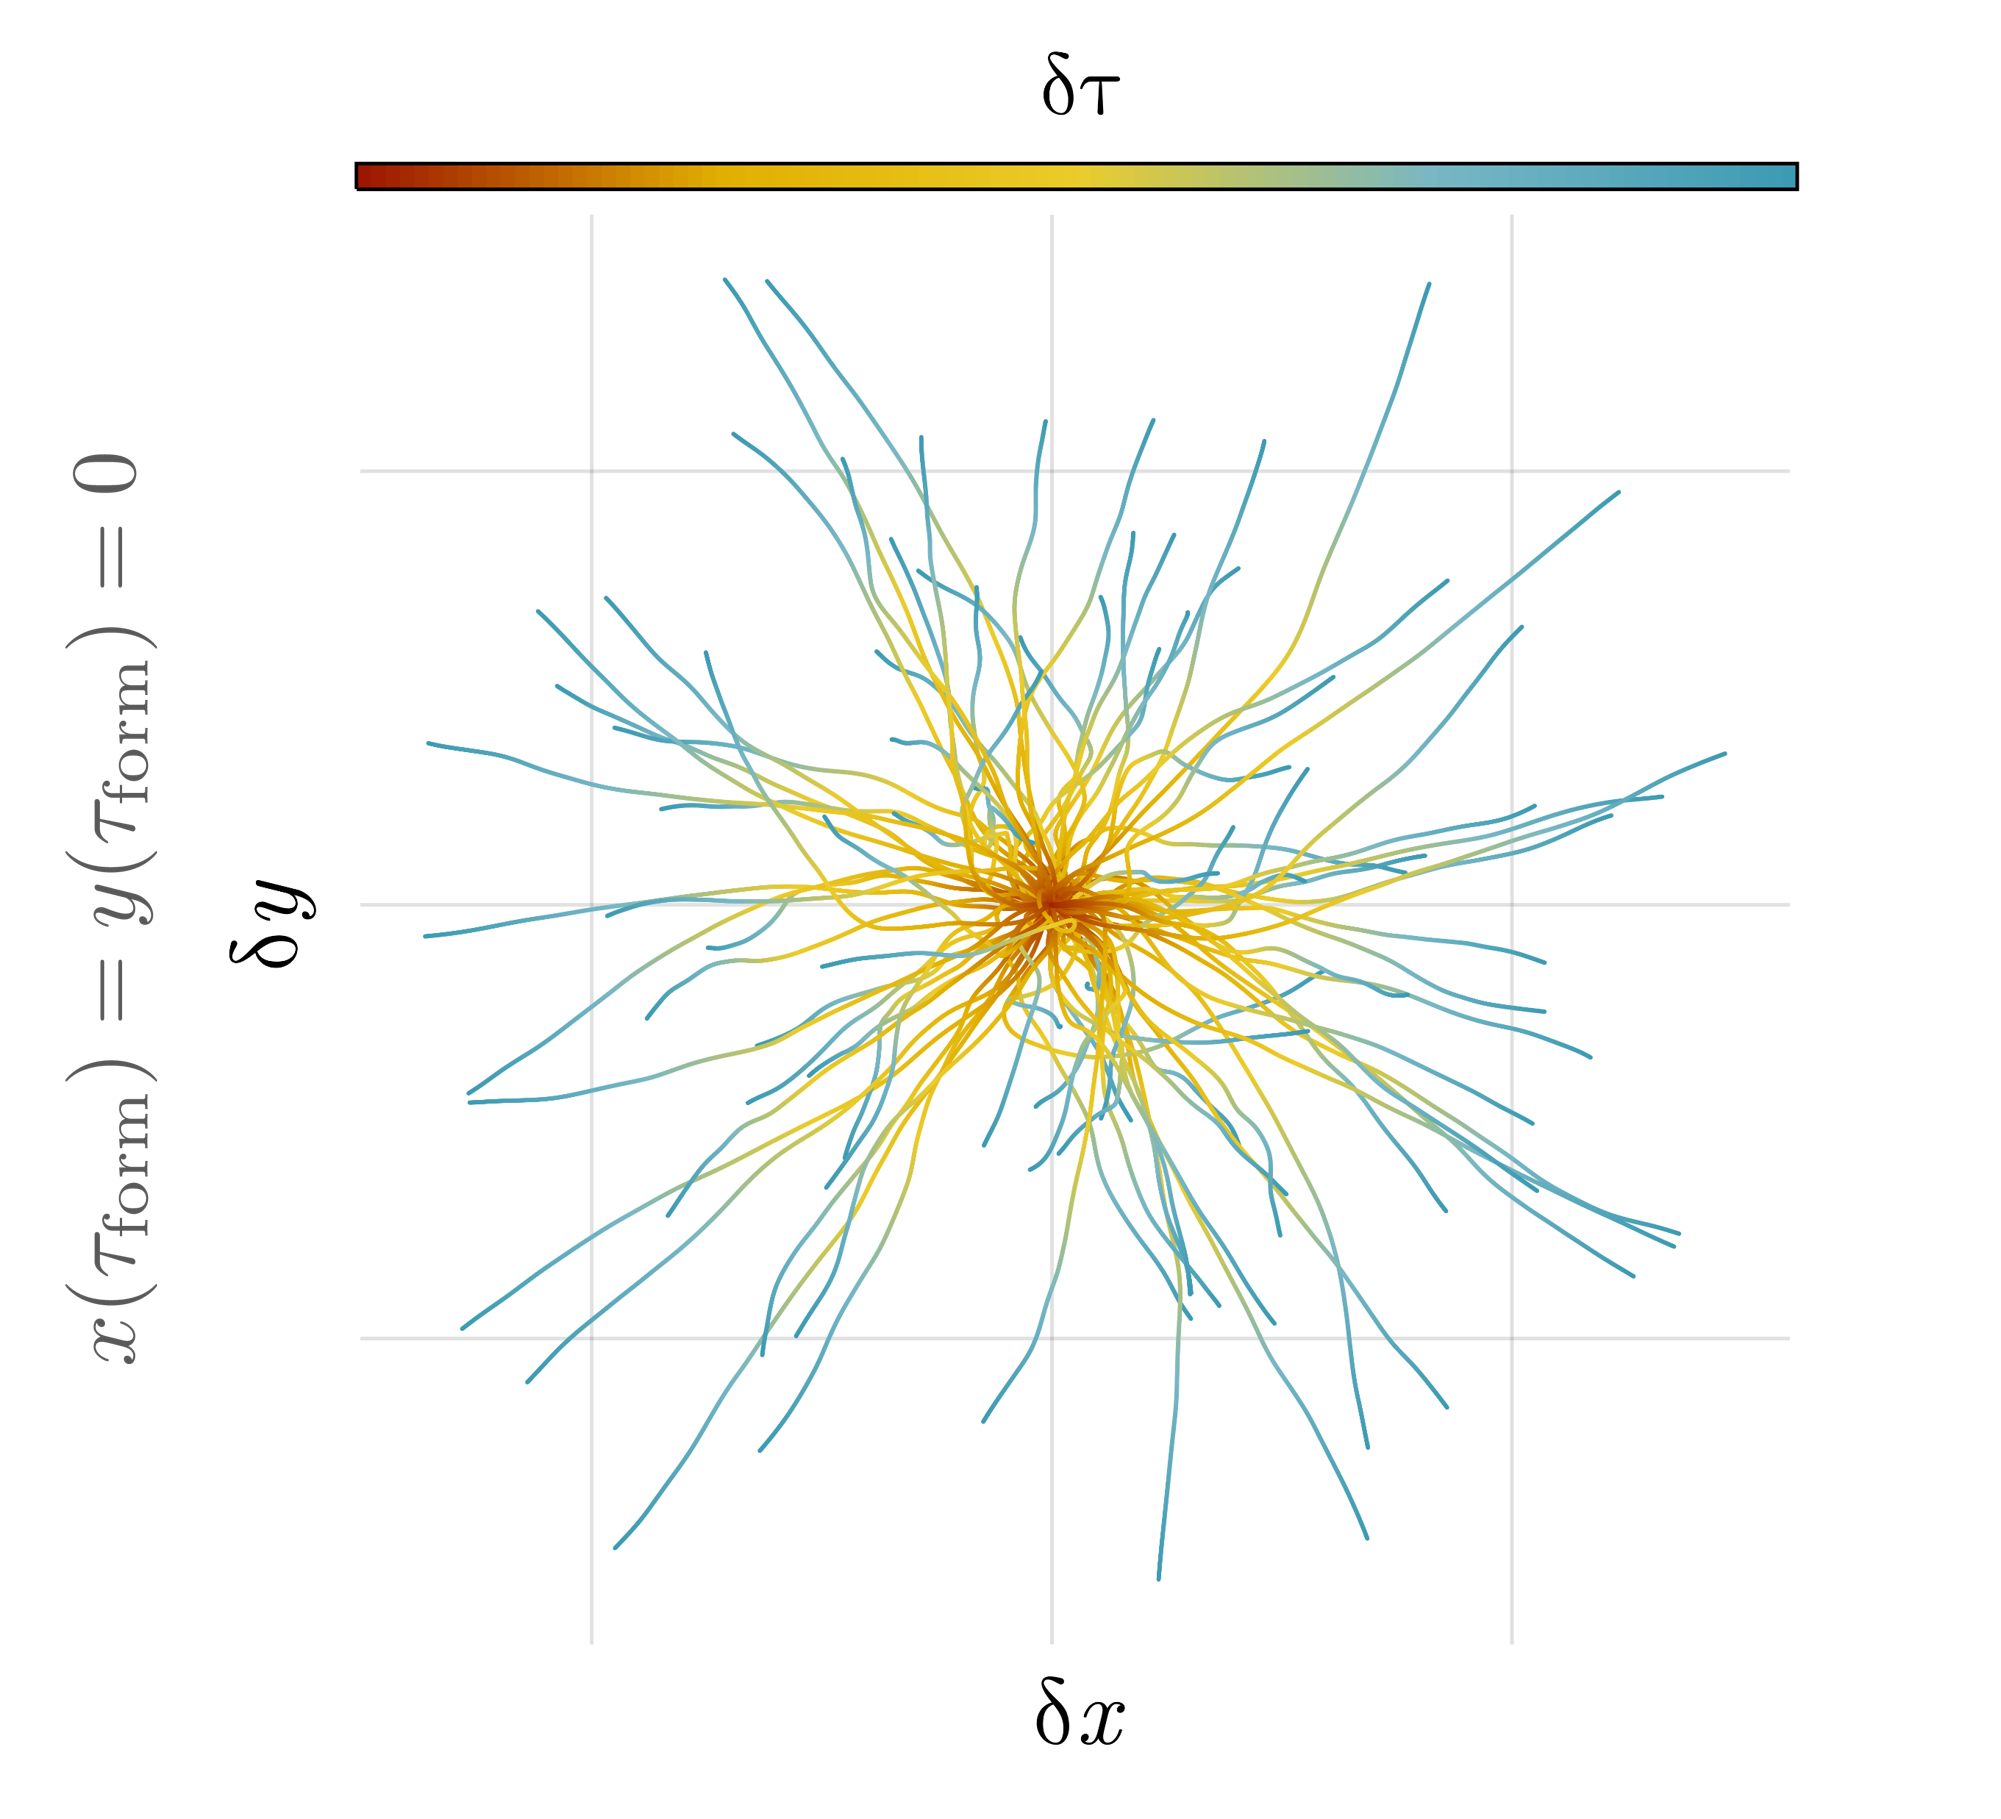
\includegraphics[width=1.1\columnwidth]{images/wong_coord.png}
                \end{figure}
                \column{.025\textwidth}
        \column{.3\textwidth}
            \begin{itemize}\itemsep0em 
                \setbeamertemplate{itemize item}{\raisebox{0.2em}{\scalebox{0.7}{${\color{normal}\blacktriangleright}$}}} 
                \item \begin{center}\footnotesize {\bfseries Momentum} broadening due to color Lorentz force\end{center}
            \end{itemize}
            \vspace{-20pt}
            \begin{figure}[!hbt]
                \centering
                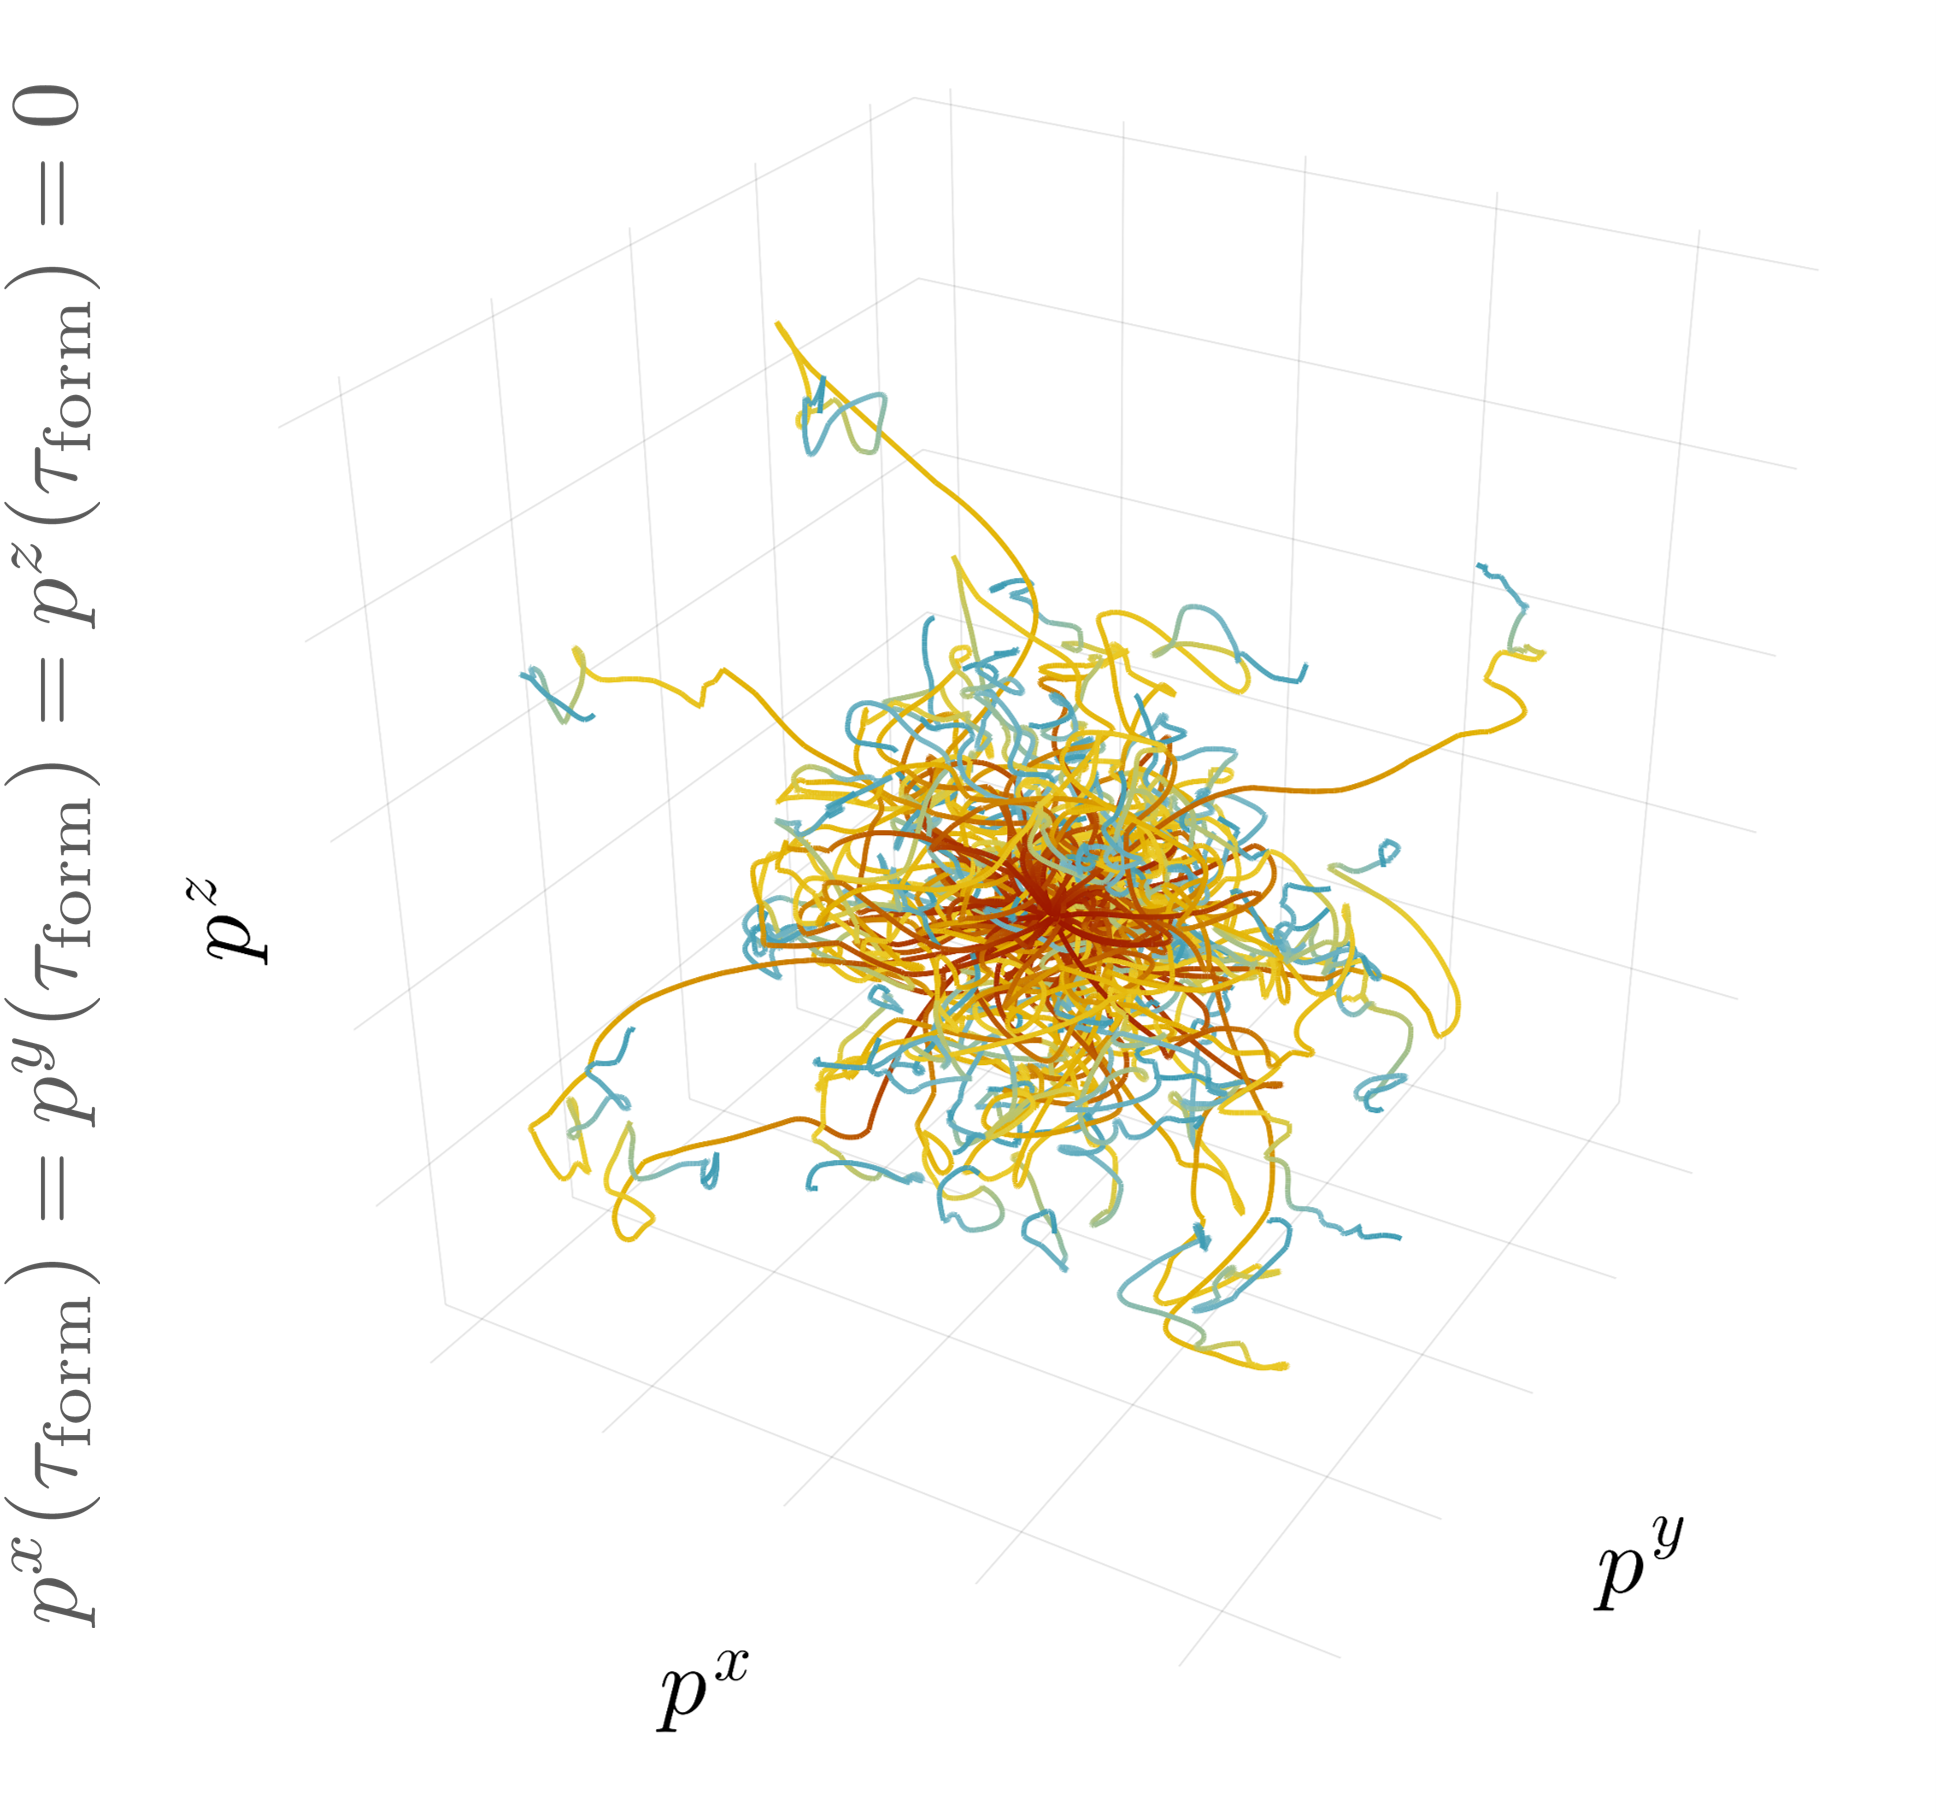
\includegraphics[width=1.1\columnwidth]{images/wong_mom.png}
            \end{figure}
            \column{.025\textwidth}
        \column{.3\textwidth}
            \begin{itemize}\itemsep0em 
                \setbeamertemplate{itemize item}{\raisebox{0.2em}{\scalebox{0.7}{${\color{normal}\blacktriangleright}$}}} 
                \item \begin{center}\footnotesize {\bfseries Color charge} rotation in SU(3) with Wilson lines\end{center}
            \end{itemize}
            \vspace{-15pt}
            \begin{figure}[!hbt]
                \centering
                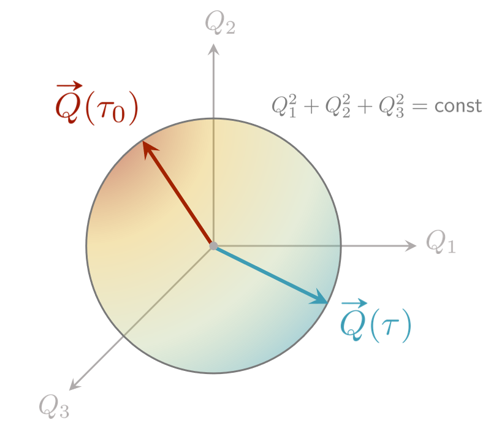
\includegraphics[width=1.05\columnwidth]{images/wong_charge.png}
            \end{figure}
            \column{.025\textwidth}
    \end{columns}

    \blfootnote{\scriptsize DA, Băran, Greco, Ipp, Müller, Ruggieri  \href{https://arxiv.org/abs/2303.05599}{{\color{palgold}\texttt{[2303.05599]}$^\text{\scalebox{0.9}{\faExternalLink}}$}}}
\end{frame}



% %%%%%%%%%%%%%%%%%%%%%%%%%%%%%%%%%%%%%%%%%
% %%%%%%%%%%%%%%%%% SLIDE %%%%%%%%%%%%%%%%%
% %%%%%%%%%%%%%%%%%%%%%%%%%%%%%%%%%%%%%%%%%

\begin{frame}
    \frametitle{Boltzmann-Vlasov equations}
    % \framesubtitle{Boltzmann-Vlasov equations}
        \setbeamertemplate{itemize item}{\raisebox{0.2em}{\scalebox{0.7}{${\color{ming}\blacktriangleright}$}}} 
   \begin{center}
    \begin{custombox2}{Classical transport equations}{lightgray}
        \small
        \begin{varwidth}{0.76\textwidth}
        \begin{itemize}\itemsep0em 
            \setbeamertemplate{itemize item}{\raisebox{0.2em}{\scalebox{0.7}{${\color{lightgray}\blacktriangleright}$}}} 
            \item Wong's equations $\leftrightarrow$ equations of motion for test particles $({\color{customblue}x^\mu},{\color{customred}p^\mu},{\color{customyellow}Q})$\\
            probing a distribution function $\boldsymbol{f}({\color{customblue}x^\mu}, {\color{customred}p^\mu}, {\color{customyellow}Q^a})$ in a Yang-Mills field ${\color{starrysecond}A^\mu}$
        \end{itemize}
        \end{varwidth}
    \end{custombox2}

   \end{center} 
    \begin{itemize}\itemsep0em 
        \setbeamertemplate{itemize item}{\raisebox{0.1em}{\scalebox{0.7}{${\color{starrysecond}\blacktriangleright}$}}} 
        \item Boltzmann-Vlasov equation for {\color{jyured}\bfseries collisionless} non-Abelian plasma
            $${\color{customred}p^\mu}[\partial_\mu+g {\color{customyellow}Q^a} {\color{starrysecond}F^{\mu\nu}}({\color{customblue}x^\mu})\partial^\nu_{{\color{customred}p^\mu}}+gf^{abc}{\color{starrysecond}A^b_\mu}({\color{customblue}x^\mu}){\color{customyellow}Q^c}\partial_{{\color{customyellow}Q^a}}]\boldsymbol{f}({\color{customblue}x^\mu}, {\color{customred}p^\mu}, {\color{customyellow}Q^a})={\color{jyured}\boldsymbol{0}}$$
        \item $\boldsymbol{f}({\color{customblue}x^\mu}, {\color{customred}p^\mu}, {\color{customyellow}Q^a})\xrightarrow{\text{sample}}$ test particles $({\color{customblue}x^\mu}, {\color{customred}p^\mu}, {\color{customyellow}Q^a})\Rightarrow$ Wong's equations\\[10pt] 
        \item Particle current ${\color{jyured}\boldsymbol{j^\mu}}\xleftrightarrow{\text{couple}}$ fields $\mathcal{D}_\mu F^{\mu\nu}[{\color{starrysecond}A^a_\mu}]={\color{jyured}\boldsymbol{j^\nu}}({\color{customblue}x^\mu}, {\color{customred}p^\mu}, {\color{customyellow}Q^a})$\\[5pt]
        \setbeamertemplate{itemize item}{\raisebox{0.1em}{\scalebox{0.7}{${\color{jyured}\blacktriangleright}$}}} 
        \item {\bfseries\color{jyured} Couple glasma to next stages}: Boltzmann-Vlasov with collisions + color current 
    \end{itemize}
        

    % \begin{itemize}\itemsep0em 
    %     \setbeamertemplate{itemize item}{\raisebox{0.1em}{\scalebox{0.7}{${\color{starrysecond}\blacktriangleright}$}}} 
    %     \item \begin{center}\footnotesize Solve the classical transport equations with {\color{starrysecond}$A^\mu$} the {\color{starrysecond}glasma field}\end{center} 
    %     \setbeamertemplate{itemize item}{\raisebox{0.1em}{\scalebox{0.7}{${\color{palgold}\blacktriangleright}$}}} 
    %     \item \begin{center}\footnotesize Color rotation conserves ${\color{palgold}q_{2}}=Q^aQ^a$ and ${\color{palgold}q_3}=d_{abc}Q^aQ^bQ^c$ {\color{palgold}SU($3$) Casimir invariants} \end{center} 
    % \end{itemize}

    \blfootnote{\scriptsize Dumitru, Nara, Strickland \href{https://arxiv.org/abs/hep-ph/0604149}{{\color{palgold}\texttt{[hep-ph/0604149]}$^\text{\scalebox{0.9}{\faExternalLink}}$}} Mrowczynski, Schenke, Strickland \href{https://arxiv.org/abs/1603.08946}{{\color{palgold}\texttt{[1603.08946]}$^\text{\scalebox{0.9}{\faExternalLink}}$}}}
\end{frame}


%%%%%%%%%%%%%%%%%%%%%%%%%%%%%%%%%%%%%%%%%
%%%%%%%%%%%%%%%% SECTION %%%%%%%%%%%%%%%%
%%%%%%%%%%%%%%%%%%%%%%%%%%%%%%%%%%%%%%%%%

\section{Results}

%%%%%%%%%%%%%%%%%%%%%%%%%%%%%%%%%%%%%%%%%
%%%%%%%%%%%%%% SUBSECTION %%%%%%%%%%%%%%%
%%%%%%%%%%%%%%%%%%%%%%%%%%%%%%%%%%%%%%%%%

\subsection{Momentum broadening}

%%%%%%%%%%%%%%%%%%%%%%%%%%%%%%%%%%%%%%%%%
%%%%%%%%%%%%%% SUBSECTION %%%%%%%%%%%%%%%
%%%%%%%%%%%%%%%%%%%%%%%%%%%%%%%%%%%%%%%%%

\subsection{Transport coefficients}

%%%%%%%%%%%%%%%%%%%%%%%%%%%%%%%%%%%%%%%%%
%%%%%%%%%%%%%%%%% SLIDE %%%%%%%%%%%%%%%%%
%%%%%%%%%%%%%%%%%%%%%%%%%%%%%%%%%%%%%%%%%

\setbeamertemplate{background}{
\tikz[overlay,remember picture] \node[opacity=0.1, at=(current page.center), align=center] {\\[10pt]
{\transparent{0.1}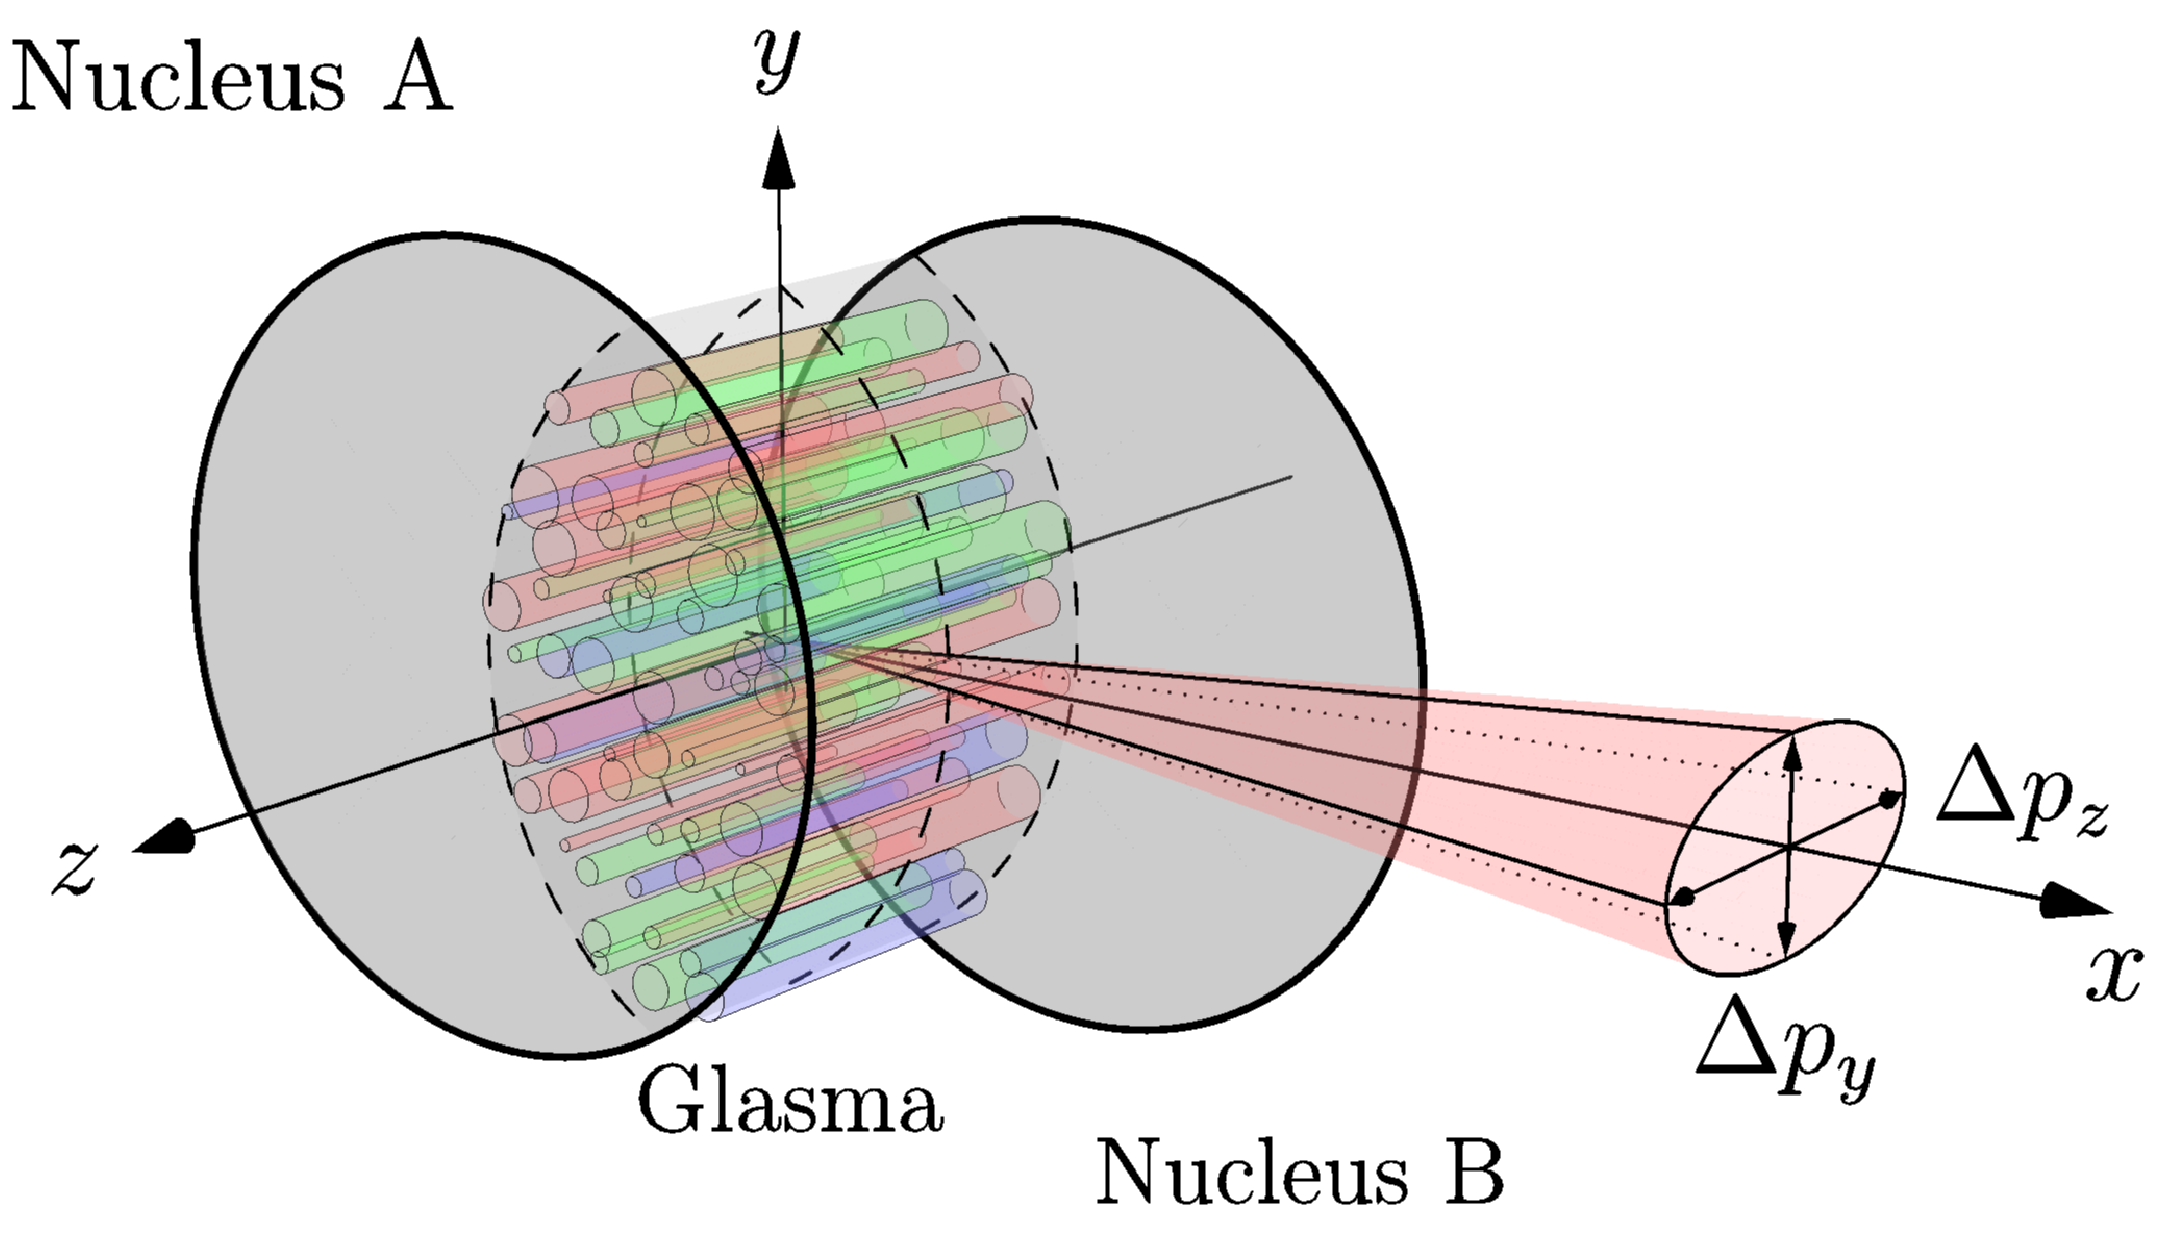
\includegraphics[height=0.7\paperheight]{images/momentum_broadening_flipped.pdf}}};
}
\setbeamertemplate{itemize item}{\raisebox{0.2em}{\scalebox{0.7}{${\color{normal}\blacktriangleright}$}}} 
\begin{frame}[plain,noframenumbering]{}
    \begin{center}
        \vspace{1cm}
        {\large\color{normal}Impact of glasma on hard probes}\\[0.3cm]
        {\huge\color{destacado}Transport coefficients}\\[0.3cm]
    \end{center}
\end{frame}
\setbeamertemplate{background}{}

%%%%%%%%%%%%%%%%%%%%%%%%%%%%%%%%%%%%%%%%%
%%%%%%%%%%%%%%%%% SLIDE %%%%%%%%%%%%%%%%%
%%%%%%%%%%%%%%%%%%%%%%%%%%%%%%%%%%%%%%%%%

\setbeamertemplate{background}{
\tikz[overlay,remember picture] \node[at=(current page.center), align=center] {\\[10pt]
{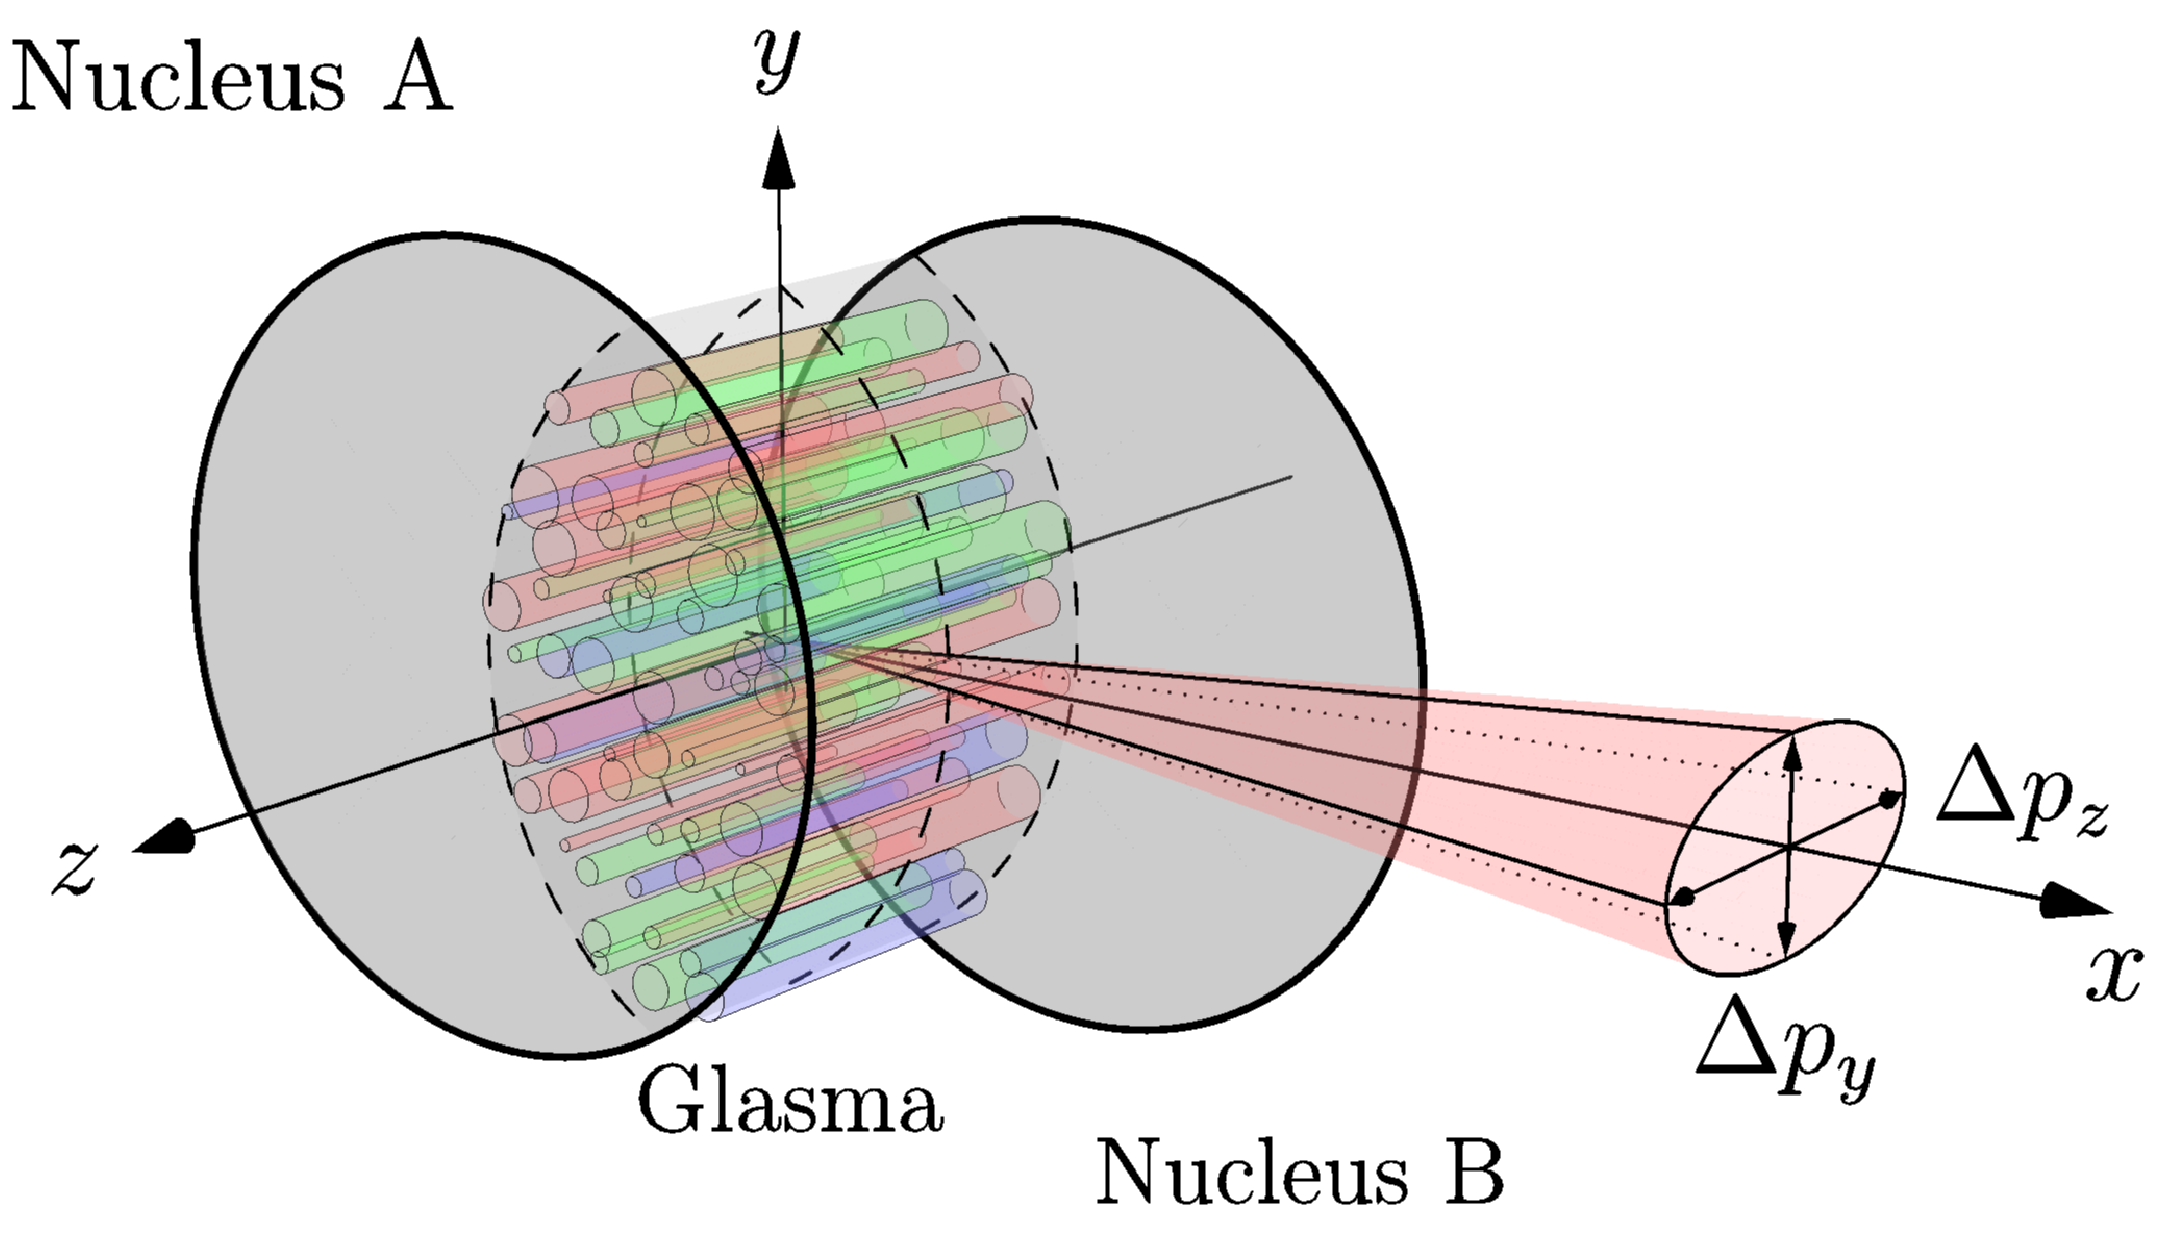
\includegraphics[height=0.7\paperheight]{images/momentum_broadening_flipped.pdf}}};
}
\setbeamertemplate{itemize item}{\raisebox{0.2em}{\scalebox{0.7}{${\color{normal}\blacktriangleright}$}}} 
\begin{frame}[plain,noframenumbering]{}
    \blfootnote{\scriptsize Ipp, Müller, Schuh \href{https://arxiv.org/abs/2009.14206}{{\color{customblue}\texttt{[2009.14206]}$^\text{\scalebox{0.9}{\faExternalLink}}$}}}
\end{frame}
\setbeamertemplate{background}{}

%%%%%%%%%%%%%%%%%%%%%%%%%%%%%%%%%%%%%%%%%
%%%%%%%%%%%%%%%%% SLIDE %%%%%%%%%%%%%%%%%
%%%%%%%%%%%%%%%%%%%%%%%%%%%%%%%%%%%%%%%%%

\begin{frame}
\frametitle{Classical transport in glasma}
% \framesubtitle{Momentum broadening, transport coefficients, anisotropy}
    \begin{columns}[onlytextwidth,t]
        \column{.45\textwidth}
            \begin{center}
                \begin{figure}
                    \centering
                    \vspace{-25pt}
                    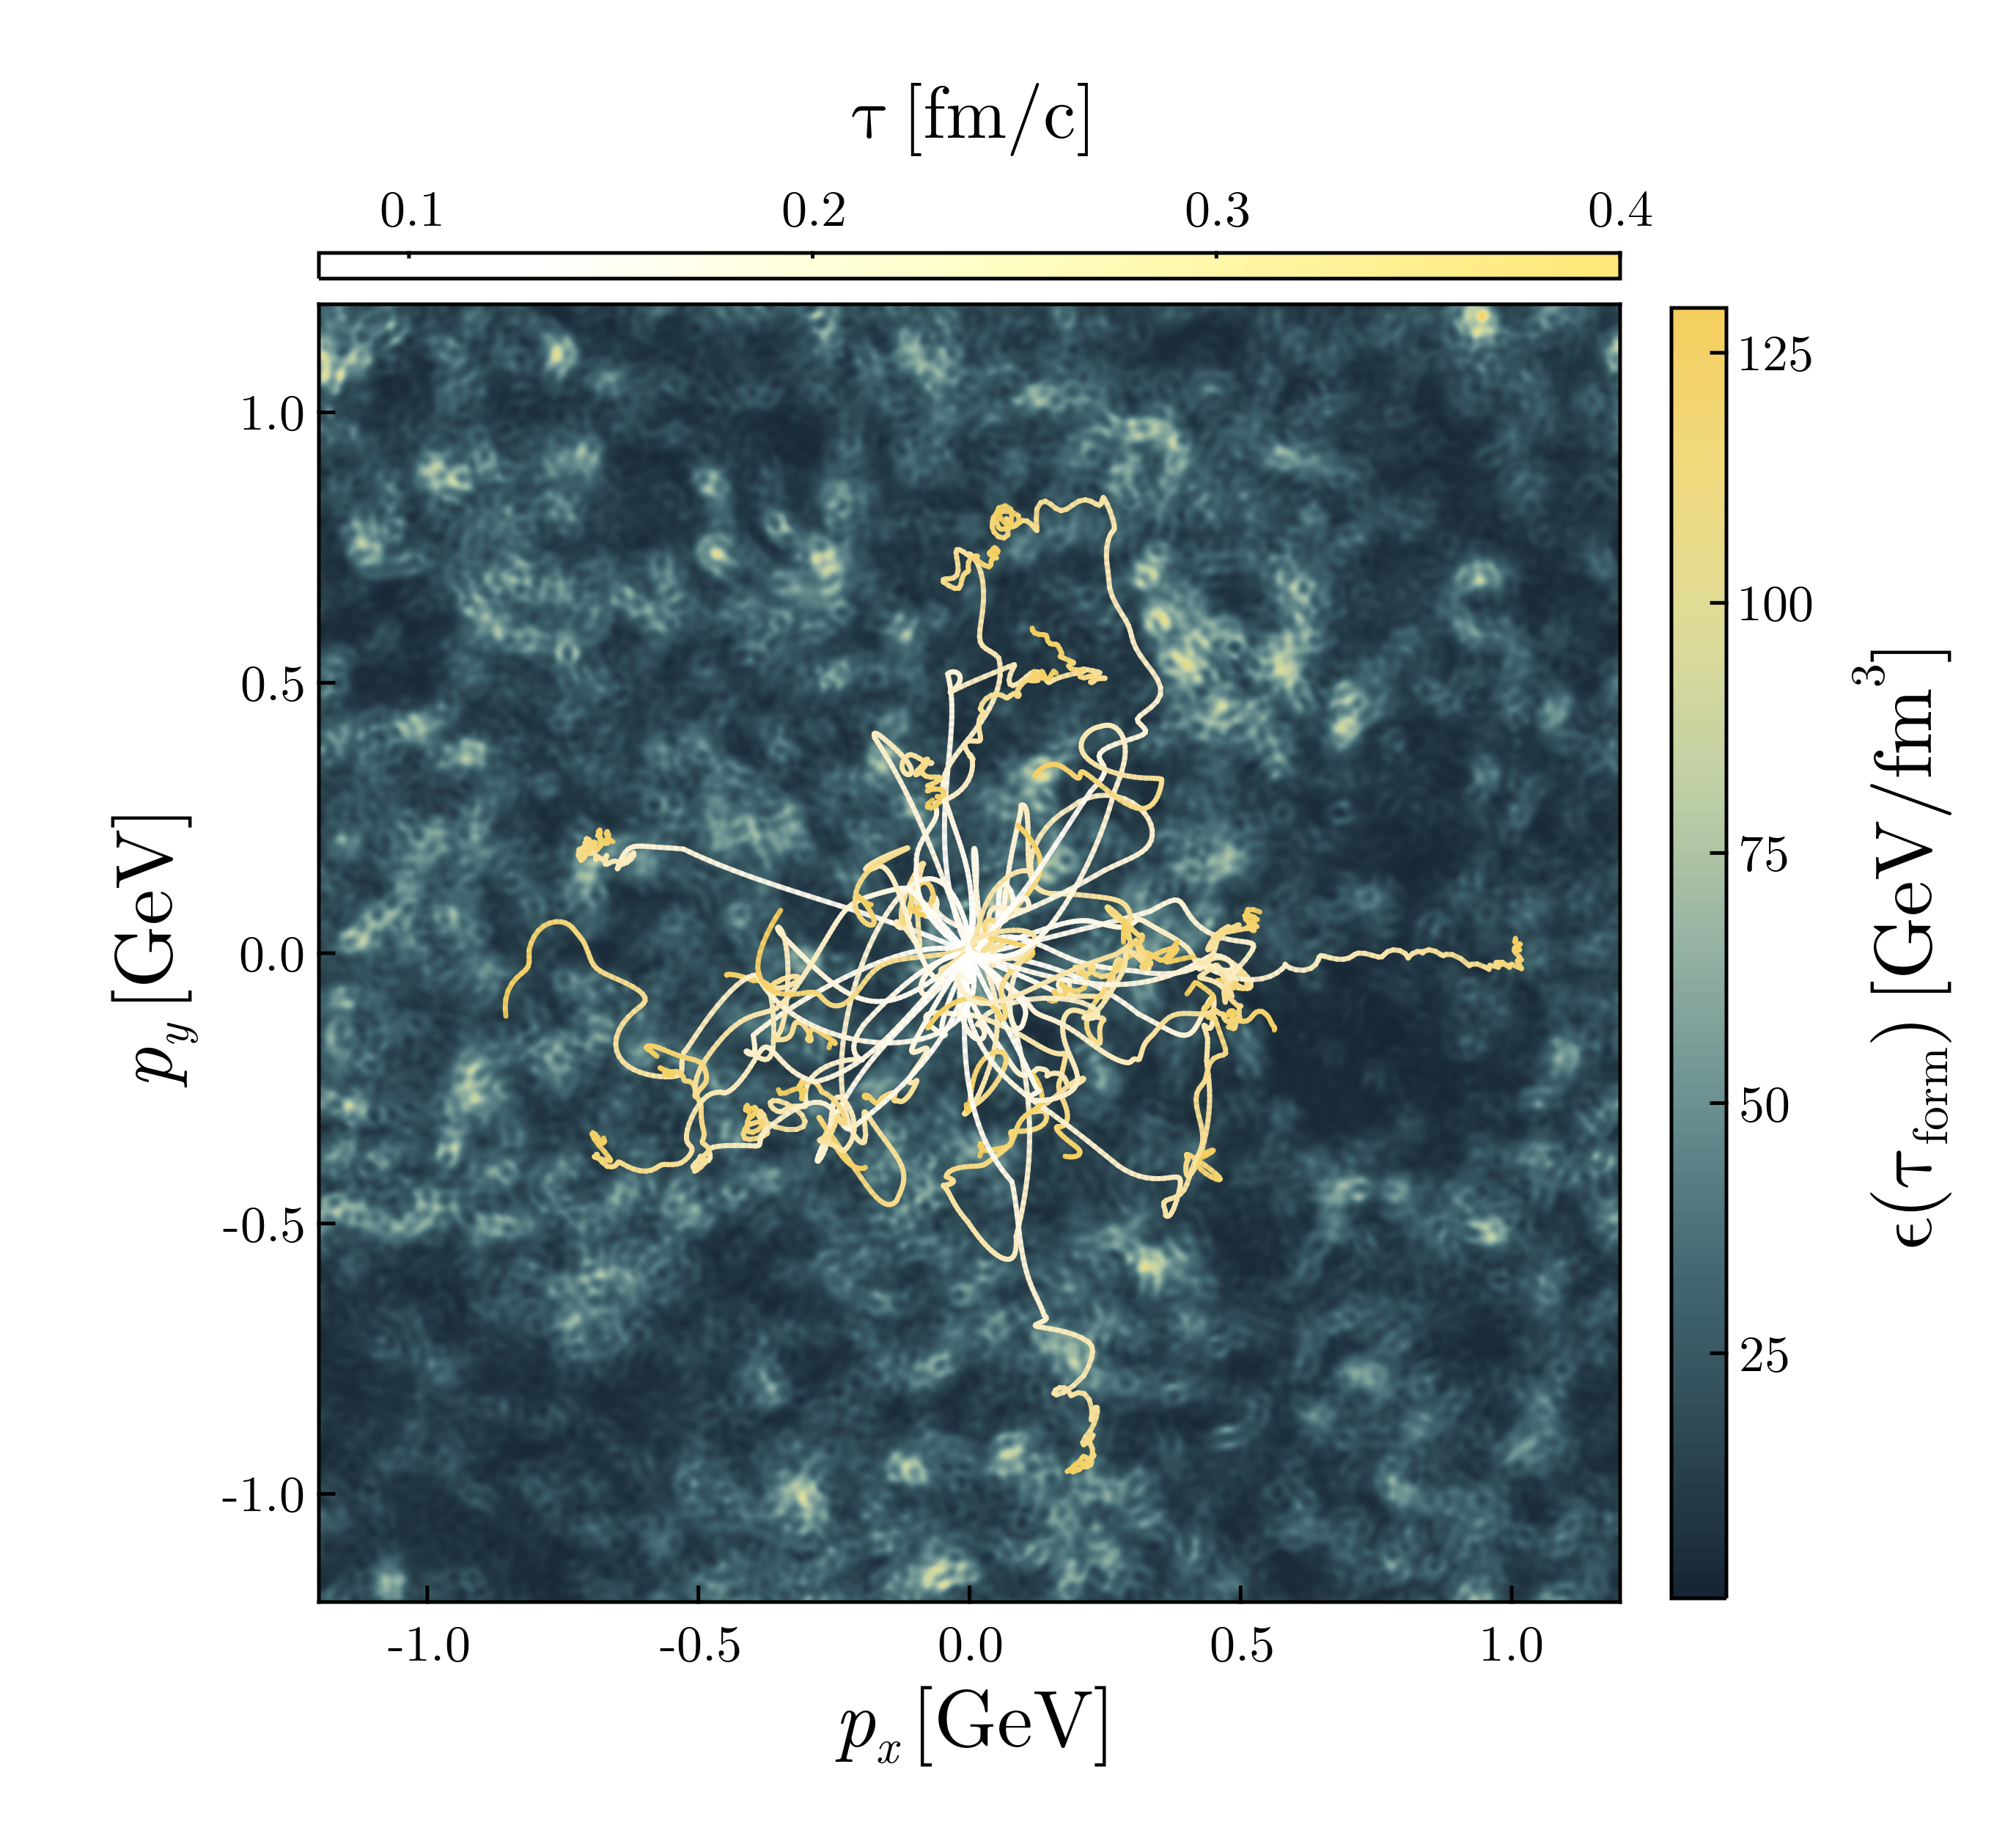
\includegraphics[width=1.15\textwidth]{images/hqs_trajectories.png}
                \end{figure}
            \end{center}
        \column{.05\textwidth}
        \column{.5\textwidth}
            \begin{center}
                \begin{custombox2}{Momentum broadening}{palteal}
                    \small
                    \begin{varwidth}{0.92\textwidth}
                    \vspace{-5pt}
                    $${\color{palteal}\boldsymbol{\delta p^2_i}}(\tau)=p^2_i(\tau)-p^2_i(\tau_\mathrm{form})$$
                    \\[-25pt]
                    {\begin{center}\scriptsize\color{lightgray} Formation time $\tau_\mathrm{form}=1/2m$ \end{center}}    
                    \vspace{-5pt}
                    \begin{itemize}\itemsep0em 
                        \setbeamertemplate{itemize item}{\raisebox{0.1em}{\scalebox{0.6}{${\color{palteal}\blacktriangleright}$}}} 
                        \item {\scriptsize Momentum kicks due to {\color{palteal}\bfseries coherent color fields}}
                        % \\[1pt] 
                        % \setbeamertemplate{itemize item}{\raisebox{0.1em}{\scalebox{0.6}{${\color{palteal}\blacktriangleright}$}}} 
                        % \item {\scriptsize Averaged over glasma and particle ensembles}
                        \vspace{3pt}
                    \end{itemize}
                    \end{varwidth}
                \end{custombox2}

                \begin{custombox2}{Transport coefficients}{customyellow}
                    \small
                    \begin{varwidth}{0.92\textwidth}
                        \vspace{-12pt}
                    $$\frac{\d }{\d\tau}\langle {\color{palteal}\boldsymbol{\delta p^2_i}}(\tau)\rangle= \begin{cases}{\color{customyellow}\boldsymbol{\kappa_i}}(\tau),&\text{heavy quarks}\\
                        {\color{customyellow}\boldsymbol{\hat{q}_i}}(\tau),&\text{jets}\end{cases}$$
                    \\[-30pt]
                    {\begin{center}\scriptsize\color{lightgray} $\langle \quad\rangle$ averaged over glasma and particle ensembles\end{center}}    
                    \vspace{-15pt}
                    \begin{itemize}\itemsep0em 
                        \setbeamertemplate{itemize item}{\raisebox{0.1em}{\scalebox{0.6}{${\color{customyellow}\blacktriangleright}$}}} 
                        \item {\scriptsize Different interpretation than standard $\kappa$, $\hat{q}$}
                    \end{itemize}
                    \end{varwidth}
                \end{custombox2}

                \begin{custombox2}{Momentum anisotropy}{starrymain}
                    \small
                    \begin{varwidth}{0.95\textwidth}
                        \vspace{-3pt}
                    % \vspace{-20pt}
                    \begin{itemize}\itemsep0em 
                        \setbeamertemplate{itemize item}{\raisebox{0.1em}{\scalebox{0.6}{${\color{starrymain}\blacktriangleright}$}}} 
                        \item {\scriptsize Longitudinal $L$ $\neq$ transverse $T$ $\Rightarrow$ ${\color{starrymain}\langle\boldsymbol{\delta p_L^2}\rangle/\langle\boldsymbol{\delta p_T^2}\rangle}$}
                    \end{itemize}
                    \end{varwidth}
                \end{custombox2}
        \end{center}
    \end{columns}
    \end{frame}


%%%%%%%%%%%%%%%%%%%%%%%%%%%%%%%%%%%%%%%%%
%%%%%%%%%%%%%%%%% SLIDE %%%%%%%%%%%%%%%%%
%%%%%%%%%%%%%%%%%%%%%%%%%%%%%%%%%%%%%%%%%

\begin{frame}
    \frametitle{Field correlators}
    % \framesubtitle{Limiting cases}
        \begin{center}
            \begin{custombox2}{Lorentz force correlator}{lightgray}
                \small
                \begin{varwidth}{0.63\textwidth}
                \begin{itemize}\itemsep0em 
                    \setbeamertemplate{itemize item}{\raisebox{0.2em}{\scalebox{0.7}{${\color{lightgray}\blacktriangleright}$}}} 
                    \item Extract momentum broadening from {\color{palteal}\bfseries force correlator}\\[5pt]
                    $\displaystyle\langle \delta p^2_i(\tau)\rangle= g^2 \int_{\tau_\mathrm{form}}^{\tau}\mathrm{d}\tau^{\prime}\int_{\tau_\mathrm{form}}^{\tau}\mathrm{d}\tau^{\prime\prime}{\color{palteal}\boldsymbol{\Big\langle \mathrm{Tr}\big[\widetilde{\mathcal{F}}_i(\tau^{\prime})\widetilde{\mathcal{F}}_i(\tau^{\prime\prime})\big]\Big\rangle}}$\\[5pt]
                    {\scriptsize\color{lightgray} Lorentz force $\mathcal{F}_i=F_{i\mu}p^\mu/E_p$ parallel transported $\widetilde{\mathcal{F}}_i$}
                \end{itemize}
                \end{varwidth}
            \end{custombox2}
        
           \end{center} 

        \begin{columns}
            \begin{column}{0.033\textwidth}\end{column}
            \begin{column}{0.4\textwidth}
                \centering
                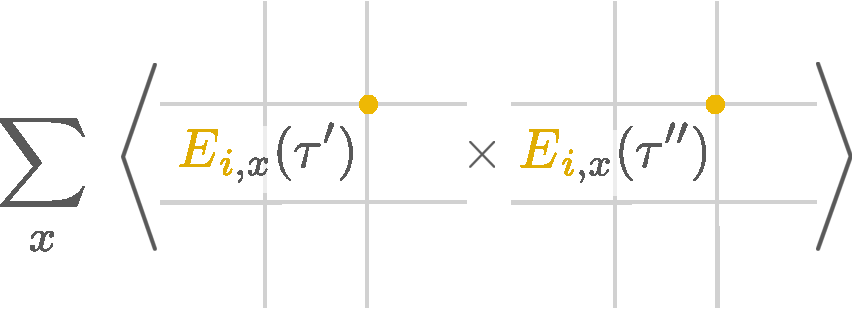
\includegraphics[width=0.9\columnwidth]{images/corr_hqs.pdf}
            \end{column}
            \begin{column}{0.01\textwidth}\end{column}
            \begin{column}{0.5\textwidth}
                % \centering
                \vspace{-10pt}
                \setbeamertemplate{itemize item}{\raisebox{0.2em}{\scalebox{0.7}{${\color{customyellow}\blacktriangleright}$}}} 
                \begin{itemize}
                    \item {\color{customyellow}\bfseries Static heavy quarks} with $m\rightarrow\infty$
                \end{itemize} 
                \vspace{7pt}
                {\footnotesize
                \begin{equation*}
                    \hspace{10pt}\langle \delta p^2_i\rangle\big|_{\color{customyellow}\boldsymbol{m\rightarrow\infty}}\propto \int\mathrm{d}\tau^{\prime}\int\mathrm{d}\tau^{\prime\prime}\Big\langle \mathrm{Tr}\big[{\color{customyellow}\boldsymbol{E_i}}(\tau^{\prime}){\color{customyellow}\boldsymbol{E_i}}(\tau^{\prime\prime})\big]\Big\rangle
                \end{equation*}}
            \end{column}
            \begin{column}{0.056\textwidth}\end{column}
        \end{columns}

        \begin{columns}
            \begin{column}{0.033\textwidth}\end{column}
            \begin{column}{0.4\textwidth}
                \centering
                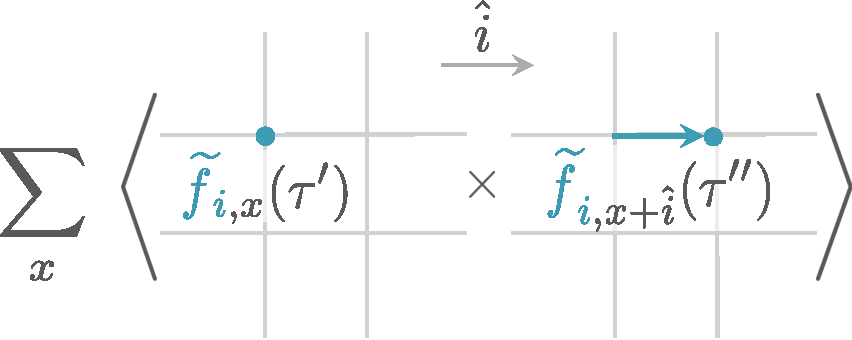
\includegraphics[width=0.9\columnwidth]{images/corr_jets.pdf}
            \end{column}
            \begin{column}{0.01\textwidth}\end{column}
            \begin{column}{0.5\textwidth}
                % \centering
                \vspace{-10pt}
                \setbeamertemplate{itemize item}{\raisebox{0.2em}{\scalebox{0.7}{${\color{customblue}\blacktriangleright}$}}} 
                \begin{itemize}
                    \item {\color{customblue}\bfseries Eikonal jets} with $p^x\rightarrow\infty$
                \end{itemize} 
                \vspace{7pt}
                {\footnotesize
                \begin{equation*}
                    \hspace{10pt}\langle \delta p^2_i\rangle\big|_{\color{customblue}\boldsymbol{p^x\rightarrow\infty}}\propto \int\mathrm{d}\tau^{\prime}\int\mathrm{d}\tau^{\prime\prime}\Big\langle \mathrm{Tr}\big[{\color{customblue}\boldsymbol{\widetilde{f}_i}}(\tau^{\prime}){\color{customblue}\boldsymbol{\widetilde{f}_i}}(\tau^{\prime\prime})\big]\Big\rangle
                \end{equation*}}
                {\scriptsize\color{lightgray} \hspace{18pt}$f_y=E_y-B_z$, $f_z=E_z+B_y$}
            \end{column}
            \begin{column}{0.056\textwidth}\end{column}
        \end{columns}
    \begin{tikzpicture}[overlay, remember picture]
        \node[anchor=north west] 
        at ([xshift=0.05cm,yshift=-0.05cm]current page.north west) {\begin{talkbox}\scriptsize{\color{destacado}Mrowczynski$\hspace{1pt}^\text{\scalebox{0.9}{\faComment}}$} {\itshape Tue 9:00$\hspace{1pt}^\text{\scalebox{0.9}{\faClockO}}$} \end{talkbox}};
    \end{tikzpicture}
    \begin{tikzpicture}[overlay, remember picture]
        \node[anchor=north west] 
        at ([xshift=0.05cm,yshift=-0.48cm]current page.north west) {\begin{talkbox}\scriptsize{Field correlators} \end{talkbox}};
    \end{tikzpicture}
    \begin{tikzpicture}[overlay, remember picture]
        \node[anchor=north west] 
        at ([xshift=0.05cm,yshift=-1.05cm]current page.north west) {\begin{talkbox}\scriptsize{\color{destacado}Ipp$\hspace{1pt}^\text{\scalebox{0.9}{\faComment}}$} {\itshape Tue 14:30$\hspace{1pt}^\text{\scalebox{0.9}{\faClockO}}$} \end{talkbox}};
    \end{tikzpicture}
    \begin{tikzpicture}[overlay, remember picture]
        \node[anchor=north west] 
        at ([xshift=0.05cm,yshift=-1.48cm]current page.north west) {\begin{talkbox}\scriptsize{Eikonal jets} \end{talkbox}};
    \end{tikzpicture}
\end{frame}



%%%%%%%%%%%%%%%%%%%%%%%%%%%%%%%%%%%%%%%%%
%%%%%%%%%%%%%%%%% SLIDE %%%%%%%%%%%%%%%%%
%%%%%%%%%%%%%%%%%%%%%%%%%%%%%%%%%%%%%%%%%

\begin{frame}[t]
    \frametitle{Literature timeline}
    \begin{center}
        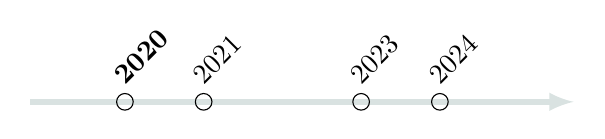
\begin{tikzpicture}[xscale=1]
            \draw[line width=0.7mm,-latex,palteal!20] (-0.2,0) -- (6.5+0.2,0);
            \foreach \X [evaluate=\X as \Y using int(\X-2019),count=\Z] in {2021, 2023, 2024}
            {
            \draw[highlight on=<0>] (\Y,0) circle[radius=3pt];
            \node[anchor=south,highlight on=<0>,fill=white,rotate=45,anchor=south
            west,inner sep=0pt] at (\Y,0.2) {\X};
            }
            \foreach \X [evaluate=\X as \Y using int(\X-2019),count=\Z] in {2020}
            {
            \draw[highlight on=<\Z>] (\Y,0) circle[radius=3pt];
            \node[anchor=south,highlight on=<\Z>,fill=white,rotate=45,anchor=south
            west,inner sep=0pt] at (\Y,0.2) {\bfseries\X};
            }
        \end{tikzpicture}
    \end{center}
    \vspace{-10pt}
    \begin{columns}[onlytextwidth,t]
        \column{.02\textwidth}
       \column{.44\textwidth}
       \vspace{-10pt}
       \begin{figure}
            \centering
            \captionsetup{justification=centering}
            \caption{\texttt{Heavy Quarks Embedded in Glasma}}
            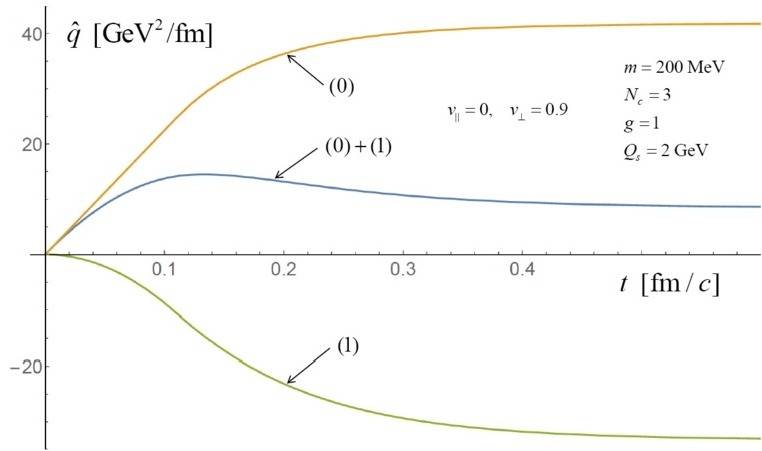
\includegraphics[width=0.95\textwidth]{images/1-s2.0-S0375947420302244-gr003_lrg (1).jpg}
        \end{figure}
        \column{.02\textwidth}
        \column{.5\textwidth}
        % \vspace{0.2cm}
        \begin{center}
            {\Large\color{palteal} Momentum broadening $\hat{q}$ \\[5pt] Collisional energy loss $\mathrm{d}E/\mathrm{d}x$ \\[10pt]}
            \footnotesize
                \begin{itemize}
                % \setbeamertemplate{itemize item}{\raisebox{0.1em}{\scalebox{0.5}{${\color{palviolet}\blacktriangleright}$}}}
                % \item {\normalsize\color{palviolet}Heavy quarks}
                \setbeamertemplate{itemize item}{\raisebox{0.1em}{\scalebox{0.5}{${\color{lightgray}\blacktriangleright}$}}}
                \item {\color{lightgray}Analytical glasma fields in $\boldsymbol{\tau}$ \textbf{expansion}}
                \item {\color{lightgray}$\langle EE\rangle$ and $\langle BB\rangle$ {\bfseries field correlators}}
                \item {\color{lightgray}{\bfseries Fokker-Planck} equation for heavy quarks}
            \end{itemize}
        \end{center}
        \column{.02\textwidth}
    \end{columns}
    \blfootnote{\scriptsize Carrington, Czajka, Mrowczynski \href{https://arxiv.org/abs/2001.05074}{\color{palgold}\texttt{[2001.05074]}$^\text{\scalebox{0.9}{\faExternalLink}}$}}
    \begin{tikzpicture}[overlay, remember picture]
        \node[anchor=north west] 
        at ([xshift=0.05cm,yshift=-0.05cm]current page.north west) {\begin{talkbox}\scriptsize{\color{destacado}Mrowczynski$\hspace{1pt}^\text{\scalebox{0.9}{\faComment}}$} {\itshape Tue 9:00$\hspace{1pt}^\text{\scalebox{0.9}{\faClockO}}$} \end{talkbox}};
    \end{tikzpicture}
\end{frame}


%%%%%%%%%%%%%%%%%%%%%%%%%%%%%%%%%%%%%%%%%
%%%%%%%%%%%%%%%%% SLIDE %%%%%%%%%%%%%%%%%
%%%%%%%%%%%%%%%%%%%%%%%%%%%%%%%%%%%%%%%%%

\begin{frame}[t,noframenumbering]
    \frametitle{Literature timeline}
    \begin{center}
        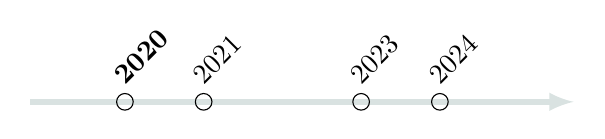
\begin{tikzpicture}[xscale=1]
            \draw[line width=0.7mm,-latex,palteal!20] (-0.2,0) -- (6.5+0.2,0);
            \foreach \X [evaluate=\X as \Y using int(\X-2019),count=\Z] in {2021, 2023, 2024}
            {
            \draw[highlight on=<0>] (\Y,0) circle[radius=3pt];
            \node[anchor=south,highlight on=<0>,fill=white,rotate=45,anchor=south
            west,inner sep=0pt] at (\Y,0.2) {\X};
            }
            \foreach \X [evaluate=\X as \Y using int(\X-2019),count=\Z] in {2020}
            {
            \draw[highlight on=<\Z>] (\Y,0) circle[radius=3pt];
            \node[anchor=south,highlight on=<\Z>,fill=white,rotate=45,anchor=south
            west,inner sep=0pt] at (\Y,0.2) {\bfseries\X};
            }
        \end{tikzpicture}
    \end{center}
    \vspace{-10pt}
    \begin{columns}[onlytextwidth,t]
        \column{.02\textwidth}
       \column{.44\textwidth}
       \vspace{-13pt}
       \begin{figure}
            \centering
            \captionsetup{justification=centering}
            \caption{\texttt{Heavy quark diffusion in an \\overoccupied gluon plasma}}
            \vspace{-10pt}
            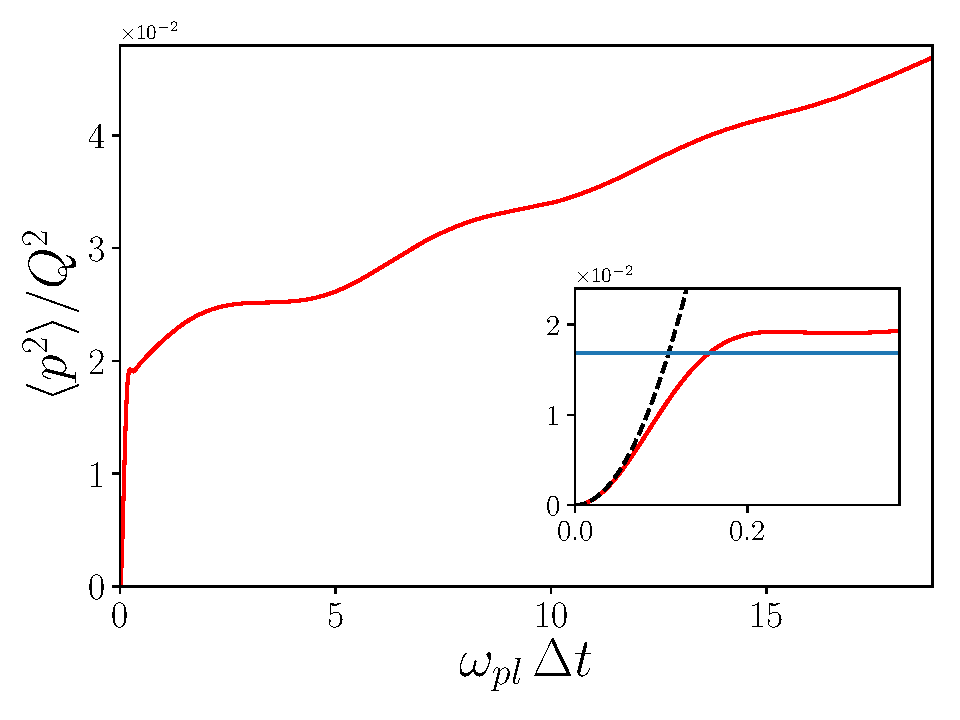
\includegraphics[width=0.9\textwidth]{images/mombroadening_with_inset_and_approximations.pdf}
        \end{figure}
        \column{.02\textwidth}
        \column{.5\textwidth}
        % \vspace{0.2cm}
        \begin{center}
            \setbeamertemplate{itemize item}{\raisebox{0.1em}{\scalebox{0.5}{${\color{lightgray}\blacktriangleright}$}}}
            {\Large\color{palteal} Momentum broadening $\langle p^2 \rangle$ \\[5pt] Transport coefficient $\kappa$ } \\[10pt]
            \footnotesize
                \begin{itemize}
                \item {\footnotesize\color{lightgray}{\bfseries Over-occupied} classical Yang-Mills}
                \item {\footnotesize\color{lightgray}Numerical lattice $\boldsymbol{\langle EE\rangle}$ {\bfseries correlator}}
                \item {\footnotesize\color{lightgray}Rapid rise in $\langle p^2 \rangle$ at early $\Delta t$}
                \item {\footnotesize\color{lightgray}{\bfseries Oscillations in $\boldsymbol{\kappa$}} with plasmon frequency}
            \end{itemize}
        \end{center}
        \column{.02\textwidth}
    \end{columns}
    \blfootnote{\scriptsize Boguslavski, Kurkela, Lappi, Peuron \href{https://arxiv.org/abs/2005.02418}{\color{palgold}\texttt{[2005.02418]}$^\text{\scalebox{0.9}{\faExternalLink}}$}}
\end{frame}


%%%%%%%%%%%%%%%%%%%%%%%%%%%%%%%%%%%%%%%%%
%%%%%%%%%%%%%%%%% SLIDE %%%%%%%%%%%%%%%%%
%%%%%%%%%%%%%%%%%%%%%%%%%%%%%%%%%%%%%%%%%

\begin{frame}[t,noframenumbering]
    \frametitle{Literature timeline}
    \begin{center}
        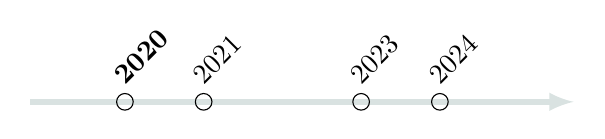
\begin{tikzpicture}[xscale=1]
            \draw[line width=0.7mm,-latex,palteal!20] (-0.2,0) -- (6.5+0.2,0);
            \foreach \X [evaluate=\X as \Y using int(\X-2019),count=\Z] in {2021, 2023, 2024}
            {
            \draw[highlight on=<0>] (\Y,0) circle[radius=3pt];
            \node[anchor=south,highlight on=<0>,fill=white,rotate=45,anchor=south
            west,inner sep=0pt] at (\Y,0.2) {\X};
            }
            \foreach \X [evaluate=\X as \Y using int(\X-2019),count=\Z] in {2020}
            {
            \draw[highlight on=<\Z>] (\Y,0) circle[radius=3pt];
            \node[anchor=south,highlight on=<\Z>,fill=white,rotate=45,anchor=south
            west,inner sep=0pt] at (\Y,0.2) {\bfseries\X};
            }
        \end{tikzpicture}
    \end{center}
    \vspace{-10pt}
    \begin{columns}[onlytextwidth,t]
        \column{.02\textwidth}
       \column{.44\textwidth}
       \vspace{-13pt}
       \begin{figure}
            \centering
            \captionsetup{justification=centering}
            \caption{\texttt{Ballistic diffusion of heavy \\ quarks in the early stage }}
            \vspace{-5pt}
            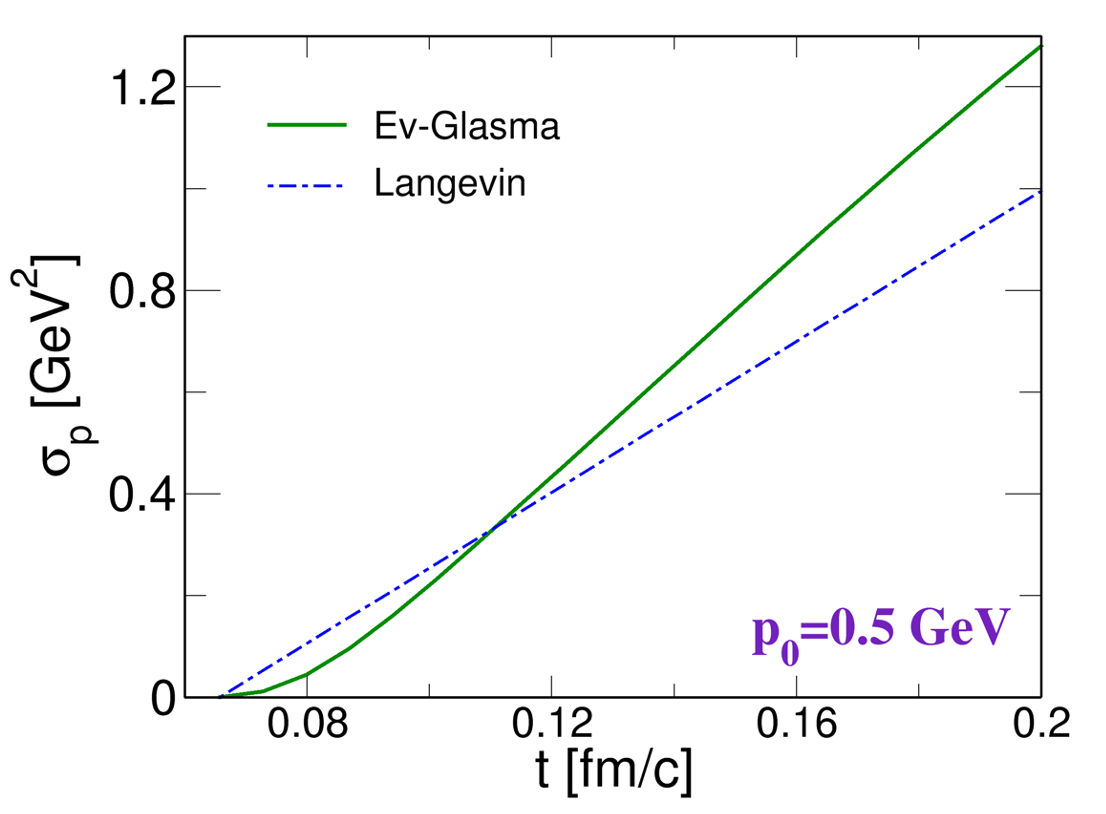
\includegraphics[width=0.85\textwidth]{images/zoom_02fm_langevin_crop.png}
        \end{figure}
        \column{.02\textwidth}
        \column{.5\textwidth}
        % \vspace{0.2cm}
        \begin{center}
            \setbeamertemplate{itemize item}{\raisebox{0.1em}{\scalebox{0.5}{${\color{lightgray}\blacktriangleright}$}}}
            {\Large\color{palteal} Momentum variance $\sigma_p$ \\[10pt]}
            \footnotesize
                \begin{itemize}
                    \item {\color{lightgray}SU(2) glasma, {\bfseries static box}}
                    \item {\color{lightgray}Numerical {\bfseries Wong's equations}}
                    \item {\color{lightgray}Dynamics compared to {\bfseries Langevin}}
                    \item {\color{lightgray}Diffusion with {\bfseries memory effects}}
                \end{itemize}
                % {\footnotesize\color{lightgray}\texttt{Ballistic diffusion of heavy quarks in \\ the early stage of relativistic heavy \\ ion collisions at RHIC and LHC}}
        \end{center}
        \column{.02\textwidth}
    \end{columns}
    \blfootnote{\scriptsize Liu, Das, Greco, Ruggieri \href{https://arxiv.org/abs/2011.05818}{\color{palgold}\texttt{[2011.05818]}$^\text{\scalebox{0.9}{\faExternalLink}}$}}
    \begin{tikzpicture}[overlay, remember picture]
        \node[anchor=north west] 
        at ([xshift=0.05cm,yshift=-0.05cm]current page.north west) {\begin{talkbox}\scriptsize{\color{destacado}Ruggieri$\hspace{1pt}^\text{\scalebox{0.9}{\faComment}}$} {\itshape Mon 11:00$\hspace{1pt}^\text{\scalebox{0.9}{\faClockO}}$} \end{talkbox}};
    \end{tikzpicture}
\end{frame}


%%%%%%%%%%%%%%%%%%%%%%%%%%%%%%%%%%%%%%%%%
%%%%%%%%%%%%%%%%% SLIDE %%%%%%%%%%%%%%%%%
%%%%%%%%%%%%%%%%%%%%%%%%%%%%%%%%%%%%%%%%%

\begin{frame}[t,noframenumbering]
    \frametitle{Literature timeline}
    \begin{center}
        \begin{tikzpicture}[xscale=1]
            \draw[line width=0.7mm,-latex,palteal!20] (-0.2,0) -- (6.5+0.2,0);
            \foreach \X [evaluate=\X as \Y using int(\X-2019),count=\Z] in {2021, 2023, 2024}
            {
            \draw[highlight on=<0>] (\Y,0) circle[radius=3pt];
            \node[anchor=south,highlight on=<0>,fill=white,rotate=45,anchor=south
            west,inner sep=0pt] at (\Y,0.2) {\X};
            }
            \foreach \X [evaluate=\X as \Y using int(\X-2019),count=\Z] in {2020}
            {
            \draw[highlight on=<\Z>] (\Y,0) circle[radius=3pt];
            \node[anchor=south,highlight on=<\Z>,fill=white,rotate=45,anchor=south
            west,inner sep=0pt] at (\Y,0.2) {\bfseries\X};
            }
        \end{tikzpicture}
    \end{center}
    \vspace{-10pt}
    \begin{columns}[onlytextwidth,t]
        \column{.02\textwidth}
       \column{.44\textwidth}
       \vspace{-13pt}
       \begin{figure}
            \centering
            \captionsetup{justification=centering}
            \caption{\texttt{Anisotropic momentum broadening \\ in the 2+1D Glasma}}
            \vspace{-15pt}
            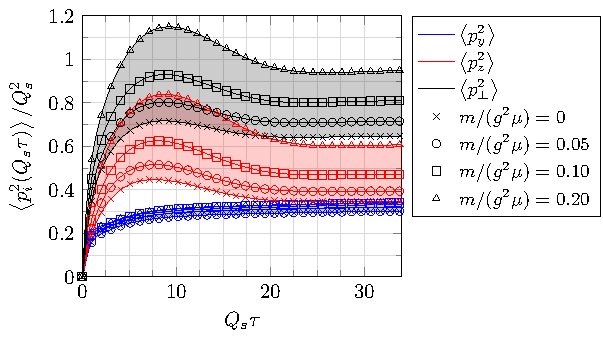
\includegraphics[width=1.05\textwidth]{images/accumulated_momentum_tau.pdf}
        \end{figure}
        \column{.02\textwidth}
        \column{.5\textwidth}
        % \vspace{0.2cm}
        \begin{center}
            \setbeamertemplate{itemize item}{\raisebox{0.1em}{\scalebox{0.5}{${\color{lightgray}\blacktriangleright}$}}}
            {\Large\color{palteal} Momentum broadening $\langle p^2\rangle$ \\[10pt]}
            \footnotesize
                \begin{itemize}
                    \item {\color{lightgray}SU(3) glasma, lattice discretization}
                    \item {\color{lightgray}{\bfseries Eikonal jets} using {\bfseries field correlators}}
                     \item {\color{lightgray}Interpretation of {\bfseries anisotropic broadening}}
                    \item {\color{lightgray}{\bfseries Weak field} analytical calculations}
                \end{itemize}
                % {\footnotesize\color{lightgray}\texttt{Ballistic diffusion of heavy quarks in \\ the early stage of relativistic heavy \\ ion collisions at RHIC and LHC}}
        \end{center}
        \column{.02\textwidth}
    \end{columns}
    \blfootnote{\scriptsize Ipp, Müller, Schuh \href{https://arxiv.org/abs/2001.10001}{\color{palgold}\texttt{[2001.10001]}$^\text{\scalebox{0.9}{\faExternalLink}}$}}
    \begin{tikzpicture}[overlay, remember picture]
        \node[anchor=north west] 
        at ([xshift=0.05cm,yshift=-0.05cm]current page.north west) {\begin{talkbox}\scriptsize{\color{destacado}Ipp$\hspace{1pt}^\text{\scalebox{0.9}{\faComment}}$} {\itshape Tue 14:30$\hspace{1pt}^\text{\scalebox{0.9}{\faClockO}}$} \end{talkbox}};
    \end{tikzpicture}
\end{frame}


%%%%%%%%%%%%%%%%%%%%%%%%%%%%%%%%%%%%%%%%%
%%%%%%%%%%%%%%%%% SLIDE %%%%%%%%%%%%%%%%%
%%%%%%%%%%%%%%%%%%%%%%%%%%%%%%%%%%%%%%%%%

\begin{frame}[t,noframenumbering]
    \frametitle{Literature timeline}
    \begin{center}
        \begin{tikzpicture}[xscale=1]
            \draw[line width=0.7mm,-latex,palteal!20] (-0.2,0) -- (6.5+0.2,0);
            \foreach \X [evaluate=\X as \Y using int(\X-2019),count=\Z] in {2021, 2023, 2024}
            {
            \draw[highlight on=<0>] (\Y,0) circle[radius=3pt];
            \node[anchor=south,highlight on=<0>,fill=white,rotate=45,anchor=south
            west,inner sep=0pt] at (\Y,0.2) {\X};
            }
            \foreach \X [evaluate=\X as \Y using int(\X-2019),count=\Z] in {2020}
            {
            \draw[highlight on=<\Z>] (\Y,0) circle[radius=3pt];
            \node[anchor=south,highlight on=<\Z>,fill=white,rotate=45,anchor=south
            west,inner sep=0pt] at (\Y,0.2) {\bfseries\X};
            }
        \end{tikzpicture}
    \end{center}
    \vspace{-10pt}
    \begin{columns}[onlytextwidth,t]
        \column{.02\textwidth}
       \column{.44\textwidth}
       \vspace{-13pt}
       \begin{figure}
            \centering
            \captionsetup{justification=centering}
            \caption{\texttt{Jet momentum broadening in the \\ pre-equilibrium Glasma
            }}
            % \vspace{-5pt}
            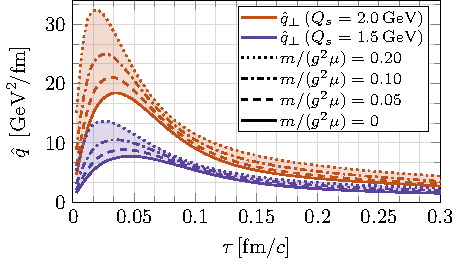
\includegraphics[width=0.95\textwidth]{images/qhat_tau.pdf}
        \end{figure}
        \column{.02\textwidth}
        \column{.5\textwidth}
        % \vspace{0.2cm}
        \begin{center}
            \setbeamertemplate{itemize item}{\raisebox{0.1em}{\scalebox{0.5}{${\color{lightgray}\blacktriangleright}$}}}
            {\Large\color{palteal} Momentum broadening $\langle p^2\rangle$ \\[5pt] Jet quenching parameter $\hat{q}$\\[10pt]}
            \footnotesize
                \begin{itemize}
                    \item {\color{lightgray}SU(3) glasma, lattice discretization}
                    \item {\color{lightgray}{\bfseries Eikonal jets} using {\bfseries field correlators}}
                     \item {\color{lightgray}Interpretation of {\bfseries anisotropic broadening}}
                    % \item {\normalsize\color{lightgray}{\bfseries Weak field} analytical calculations}
                \end{itemize}
                % {\footnotesize\color{lightgray}\texttt{Ballistic diffusion of heavy quarks in \\ the early stage of relativistic heavy \\ ion collisions at RHIC and LHC}}
        \end{center}
        \column{.02\textwidth}
    \end{columns}
    \blfootnote{\scriptsize Ipp, Müller, Schuh \href{https://arxiv.org/abs/2009.14206}{\color{palgold}\texttt{[2009.14206]}$^\text{\scalebox{0.9}{\faExternalLink}}$}}
    \begin{tikzpicture}[overlay, remember picture]
        \node[anchor=north west] 
        at ([xshift=0.05cm,yshift=-0.05cm]current page.north west) {\begin{talkbox}\scriptsize{\color{destacado}Ipp$\hspace{1pt}^\text{\scalebox{0.9}{\faComment}}$} {\itshape Tue 14:30$\hspace{1pt}^\text{\scalebox{0.9}{\faClockO}}$} \end{talkbox}};
    \end{tikzpicture}
\end{frame}


%%%%%%%%%%%%%%%%%%%%%%%%%%%%%%%%%%%%%%%%%
%%%%%%%%%%%%%%%%% SLIDE %%%%%%%%%%%%%%%%%
%%%%%%%%%%%%%%%%%%%%%%%%%%%%%%%%%%%%%%%%%

\begin{frame}[t,noframenumbering]
    \frametitle{Literature timeline}
    \begin{center}
        \begin{tikzpicture}[xscale=1]
            \draw[line width=0.7mm,-latex,palteal!20] (-0.2,0) -- (6.5+0.2,0);
            \foreach \X [evaluate=\X as \Y using int(\X-2019),count=\Z] in {2020, 2023, 2024}
            {
            \draw[highlight on=<0>] (\Y,0) circle[radius=3pt];
            \node[anchor=south,highlight on=<0>,fill=white,rotate=45,anchor=south
            west,inner sep=0pt] at (\Y,0.2) {\X};
            }
            \foreach \X [evaluate=\X as \Y using int(\X-2019),count=\Z] in {2021}
            {
            \draw[highlight on=<\Z>] (\Y,0) circle[radius=3pt];
            \node[anchor=south,highlight on=<\Z>,fill=white,rotate=45,anchor=south
            west,inner sep=0pt] at (\Y,0.2) {\bfseries\X};
            }
        \end{tikzpicture}
    \end{center}
    \vspace{-10pt}
    \begin{columns}[onlytextwidth,t]
        \column{.02\textwidth}
       \column{.44\textwidth}
       \vspace{-13pt}
       \begin{figure}
            \centering
            \captionsetup{justification=centering}
            \caption{\texttt{Heavy quarks in the early \\ stage of high energy collisions
            }}
            \vspace{-5pt}
            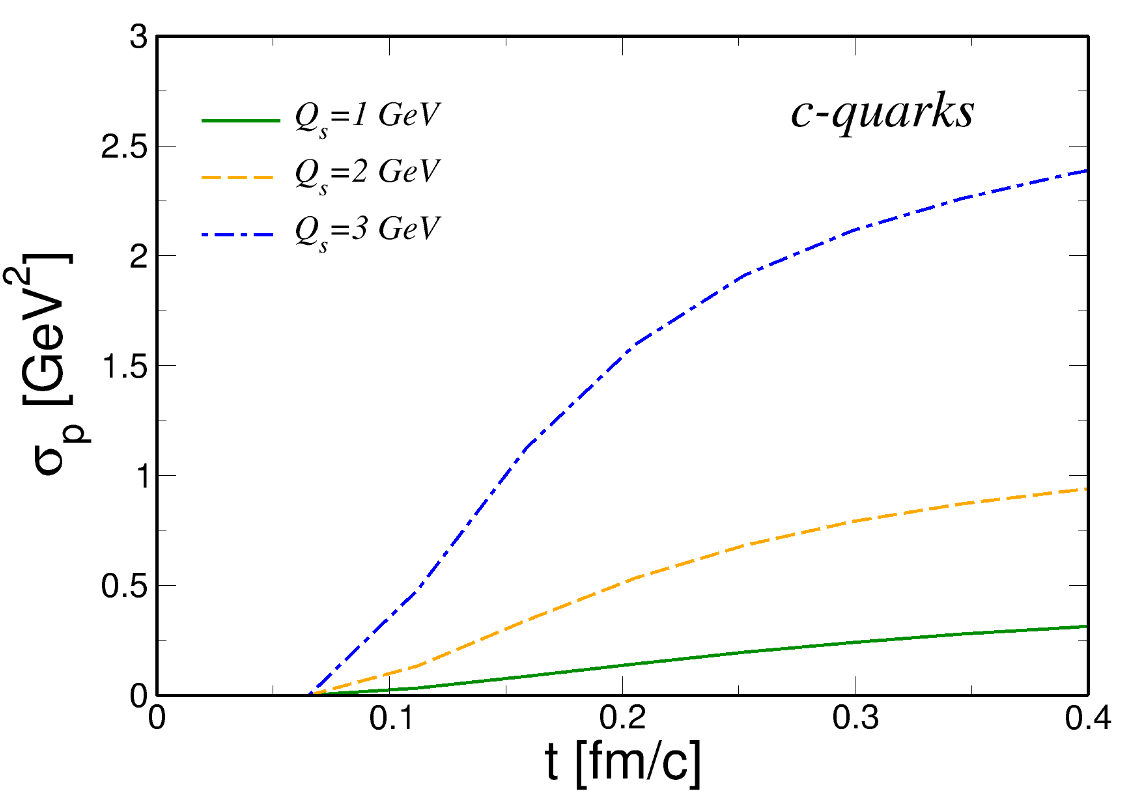
\includegraphics[width=0.9\textwidth]{images/sigmap_charm_expanding_04_crop.png}
        \end{figure}
        \column{.02\textwidth}
        \column{.5\textwidth}
        % \vspace{0.2cm}
        \begin{center}
            \setbeamertemplate{itemize item}{\raisebox{0.1em}{\scalebox{0.5}{${\color{lightgray}\blacktriangleright}$}}}
            {\Large\color{palteal} Momentum variance $\sigma_p$ \\[10pt]}
            \footnotesize
                \begin{itemize}
                    \item {\color{lightgray}SU(2) glasma, {\bfseries longitudinal expansion}}
                    \item {\color{lightgray}Numerical {\bfseries Wong's equations}}
                    \item {\color{lightgray}Dynamics compared to {\bfseries pQCD Langevin}}
                    \item {\color{lightgray}Diffusion and {\bfseries brownian motion}}
                \end{itemize}
                % {\footnotesize\color{lightgray}\texttt{Ballistic diffusion of heavy quarks in \\ the early stage of relativistic heavy \\ ion collisions at RHIC and LHC}}
        \end{center}
        \column{.02\textwidth}
    \end{columns}
    \blfootnote{\scriptsize Pooja, Das, Oliva, Ruggieri \href{https://arxiv.org/abs/2110.14610}{\color{palgold}\texttt{[2110.14610]}$^\text{\scalebox{0.9}{\faExternalLink}}$}}
    \begin{tikzpicture}[overlay, remember picture]
        \node[anchor=north west] 
        at ([xshift=0.05cm,yshift=-0.05cm]current page.north west) {\begin{talkbox}\scriptsize{\color{destacado}Ruggieri$\hspace{1pt}^\text{\scalebox{0.9}{\faComment}}$} {\itshape Mon 11:00$\hspace{1pt}^\text{\scalebox{0.9}{\faClockO}}$} \end{talkbox}};
    \end{tikzpicture}
\end{frame}



%%%%%%%%%%%%%%%%%%%%%%%%%%%%%%%%%%%%%%%%%
%%%%%%%%%%%%%%%%% SLIDE %%%%%%%%%%%%%%%%%
%%%%%%%%%%%%%%%%%%%%%%%%%%%%%%%%%%%%%%%%%

\begin{frame}[t,noframenumbering]
    \frametitle{Literature timeline}
    \begin{center}
        \begin{tikzpicture}[xscale=1]
            \draw[line width=0.7mm,-latex,palteal!20] (-0.2,0) -- (6.5+0.2,0);
            \foreach \X [evaluate=\X as \Y using int(\X-2019),count=\Z] in {2020, 2023, 2024}
            {
            \draw[highlight on=<0>] (\Y,0) circle[radius=3pt];
            \node[anchor=south,highlight on=<0>,fill=white,rotate=45,anchor=south
            west,inner sep=0pt] at (\Y,0.2) {\X};
            }
            \foreach \X [evaluate=\X as \Y using int(\X-2019),count=\Z] in {2021}
            {
            \draw[highlight on=<\Z>] (\Y,0) circle[radius=3pt];
            \node[anchor=south,highlight on=<\Z>,fill=white,rotate=45,anchor=south
            west,inner sep=0pt] at (\Y,0.2) {\bfseries\X};
            }
        \end{tikzpicture}
    \end{center}
    \vspace{-10pt}
    \begin{columns}[onlytextwidth,t]
        \column{.02\textwidth}
       \column{.44\textwidth}
       \vspace{-13pt}
       \begin{figure}
            \centering
            \captionsetup{justification=centering}
            \caption{\texttt{Jet quenching in glasma}}
            % \vspace{-5pt}
            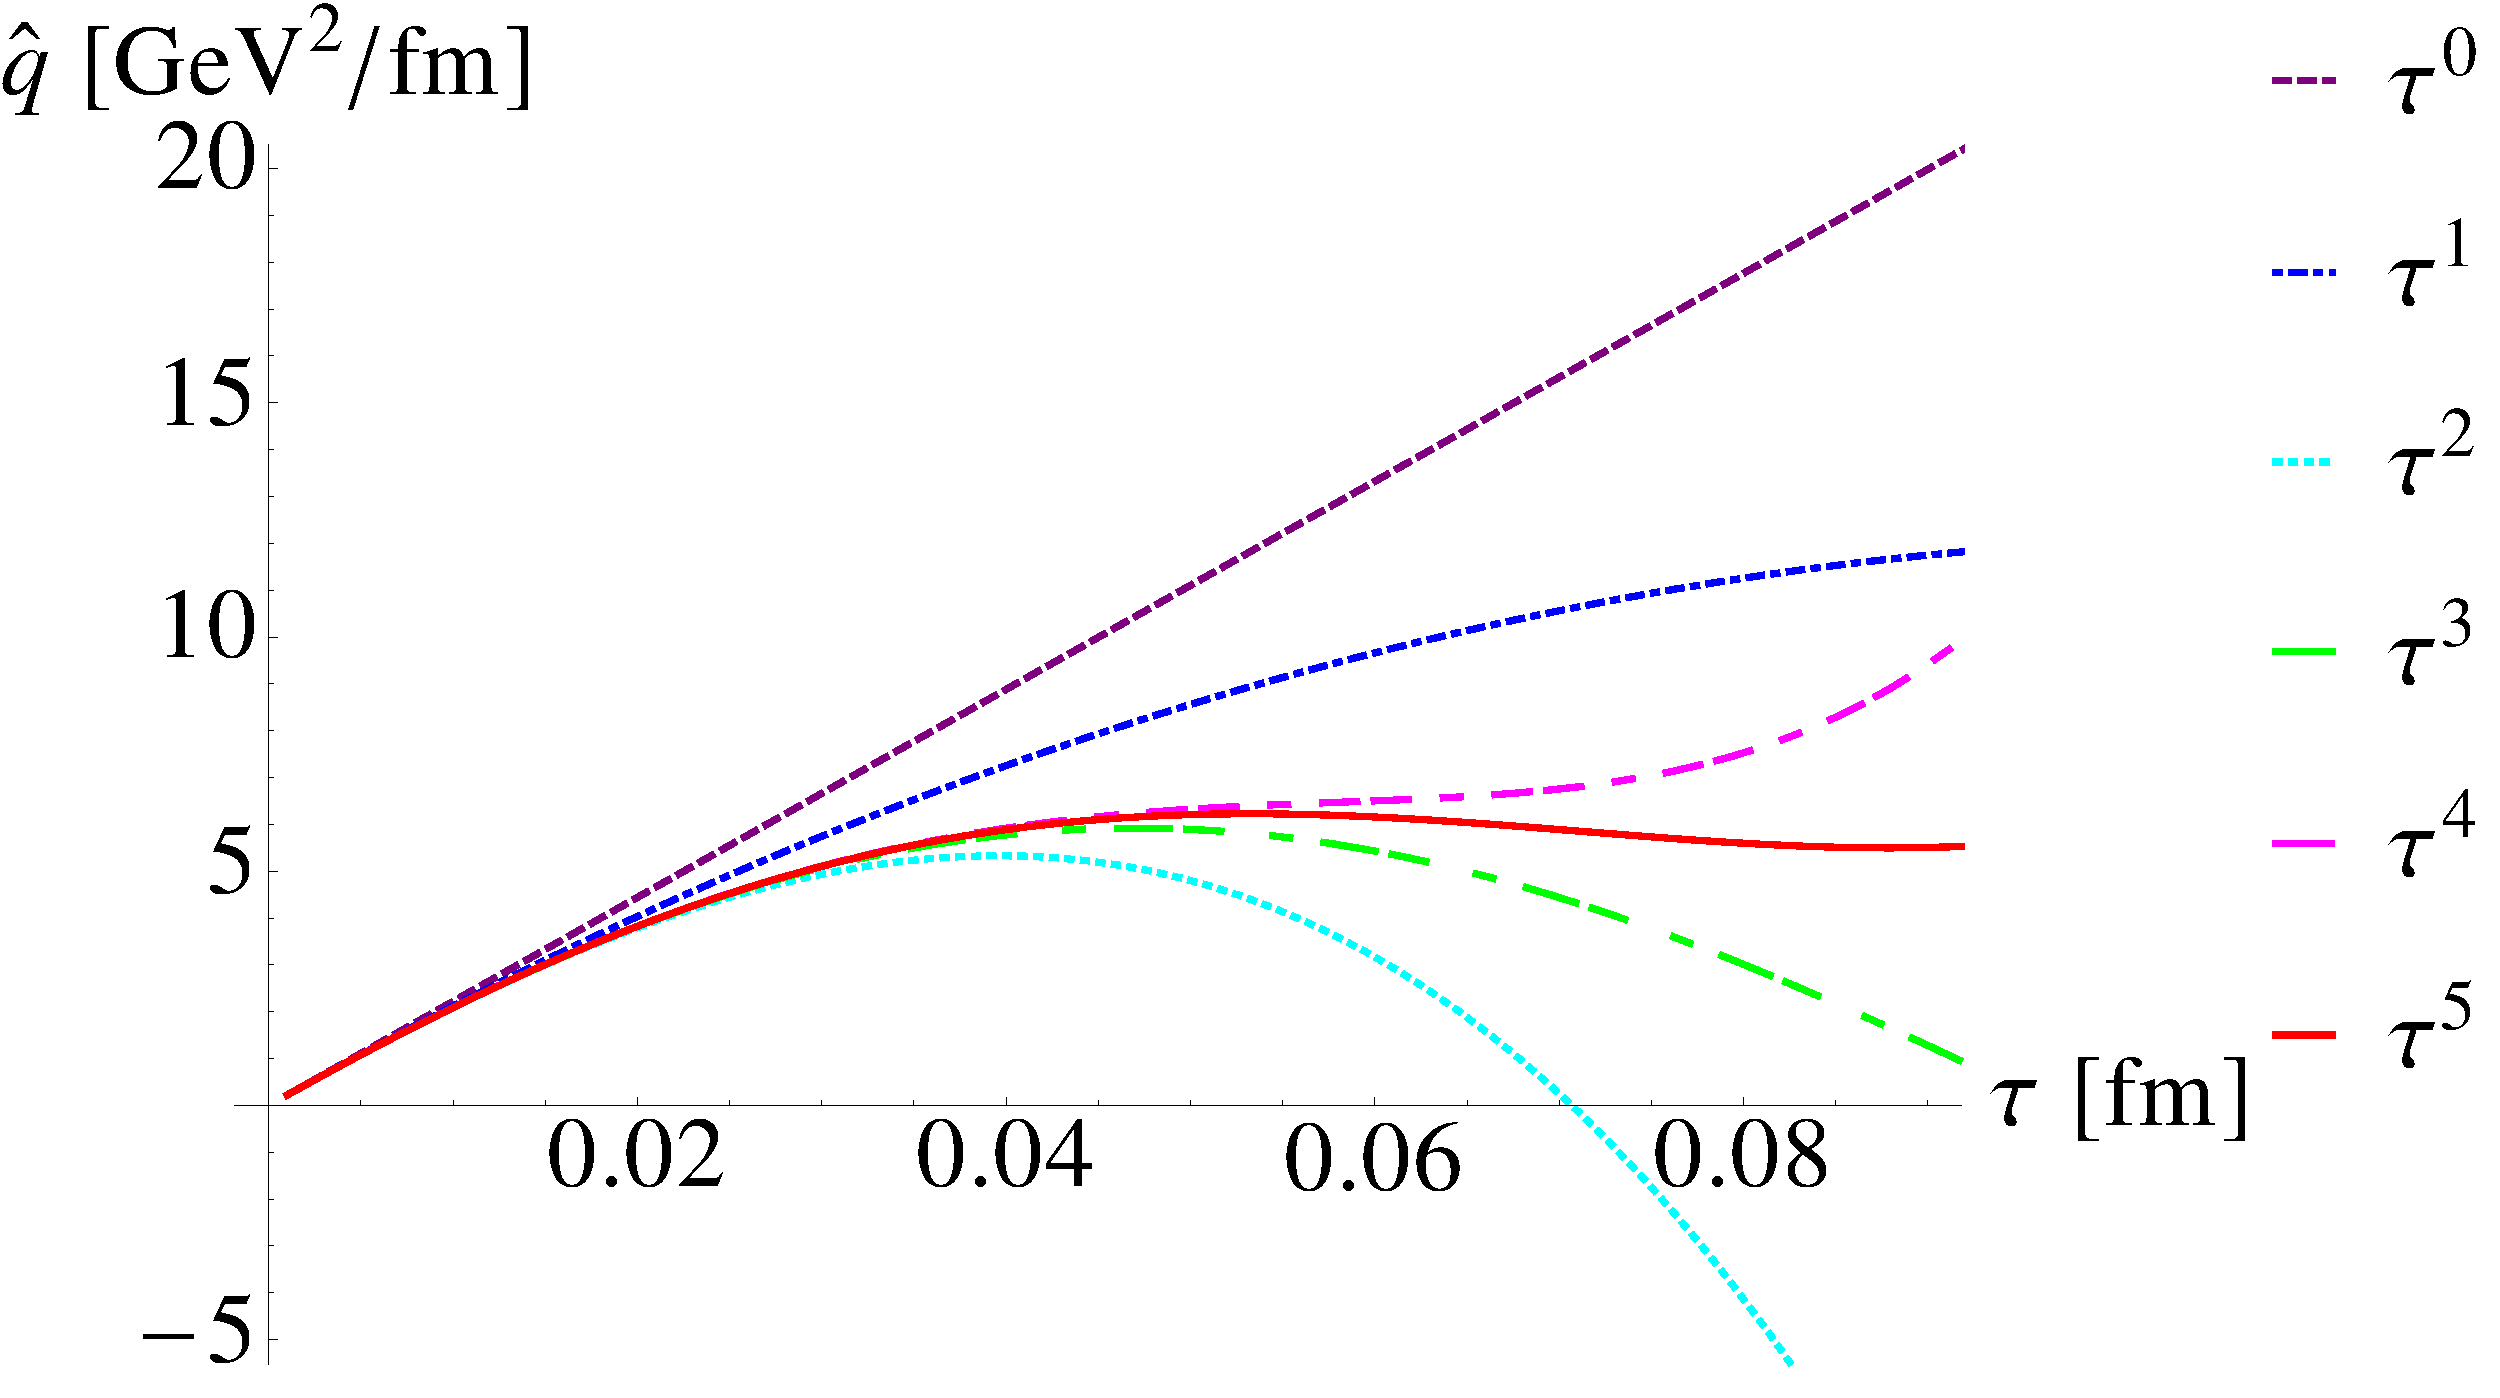
\includegraphics[width=0.95\textwidth]{images/Fig-qhat-six-cases.pdf}
        \end{figure}
        \column{.02\textwidth}
        \column{.5\textwidth}
        % \vspace{0.2cm}
        \begin{center}
            \setbeamertemplate{itemize item}{\raisebox{0.1em}{\scalebox{0.5}{${\color{lightgray}\blacktriangleright}$}}}
            {\Large\color{palteal} Momentum broadening $\Delta p_T^2$ \\[5pt] Jet quenching parameter $\hat{q}$  \\[10pt]}
            \footnotesize
                \begin{itemize}
                    \item {\color{lightgray}Analytical glasma fields in $\boldsymbol{\tau}$ \textbf{expansion}}
                    \item {\color{lightgray} {\bfseries Field correlators}, {\bfseries Fokker-Planck} equation}
                    \item {\color{lightgray} Estimate $\Delta p_T^2|^\mathrm{neq}/\Delta p_T^2|^\mathrm{eq}\approx 0.93$}
                \end{itemize}
                % {\footnotesize\color{lightgray}\texttt{Ballistic diffusion of heavy quarks in \\ the early stage of relativistic heavy \\ ion collisions at RHIC and LHC}}
        \end{center}
        \column{.02\textwidth}
    \end{columns}
    \blfootnote{\scriptsize Carrington, Czajka, Mrowczynski \href{https://arxiv.org/abs/2112.06812}{\color{palgold}\texttt{[2112.06812]}$^\text{\scalebox{0.9}{\faExternalLink}}$}}
    \begin{tikzpicture}[overlay, remember picture]
        \node[anchor=north west] 
        at ([xshift=0.05cm,yshift=-0.05cm]current page.north west) {\begin{talkbox}\scriptsize{\color{destacado}Mrowczynski$\hspace{1pt}^\text{\scalebox{0.9}{\faComment}}$} {\itshape Tue 9:00$\hspace{1pt}^\text{\scalebox{0.9}{\faClockO}}$} \end{talkbox}};
    \end{tikzpicture}
\end{frame}


%%%%%%%%%%%%%%%%%%%%%%%%%%%%%%%%%%%%%%%%%
%%%%%%%%%%%%%%%%% SLIDE %%%%%%%%%%%%%%%%%
%%%%%%%%%%%%%%%%%%%%%%%%%%%%%%%%%%%%%%%%%

\begin{frame}[t,noframenumbering]
    \frametitle{Literature timeline}
    \begin{center}
        \begin{tikzpicture}[xscale=1]
            \draw[line width=0.7mm,-latex,palteal!20] (-0.2,0) -- (6.5+0.2,0);
            \foreach \X [evaluate=\X as \Y using int(\X-2019),count=\Z] in {2020, 2021, 2024}
            {
            \draw[highlight on=<0>] (\Y,0) circle[radius=3pt];
            \node[anchor=south,highlight on=<0>,fill=white,rotate=45,anchor=south
            west,inner sep=0pt] at (\Y,0.2) {\X};
            }
            \foreach \X [evaluate=\X as \Y using int(\X-2019),count=\Z] in {2023}
            {
            \draw[highlight on=<\Z>] (\Y,0) circle[radius=3pt];
            \node[anchor=south,highlight on=<\Z>,fill=white,rotate=45,anchor=south
            west,inner sep=0pt] at (\Y,0.2) {\bfseries\X};
            }
        \end{tikzpicture}
    \end{center}
    \vspace{-10pt}
    \begin{columns}[onlytextwidth,t]
        \column{.02\textwidth}
       \column{.44\textwidth}
       \vspace{-13pt}
       \begin{figure}
            \centering
            \captionsetup{justification=centering}
            \caption{\texttt{Simulating jets and \\ heavy quarks in the Glasma}}
            \vspace{-10pt}
            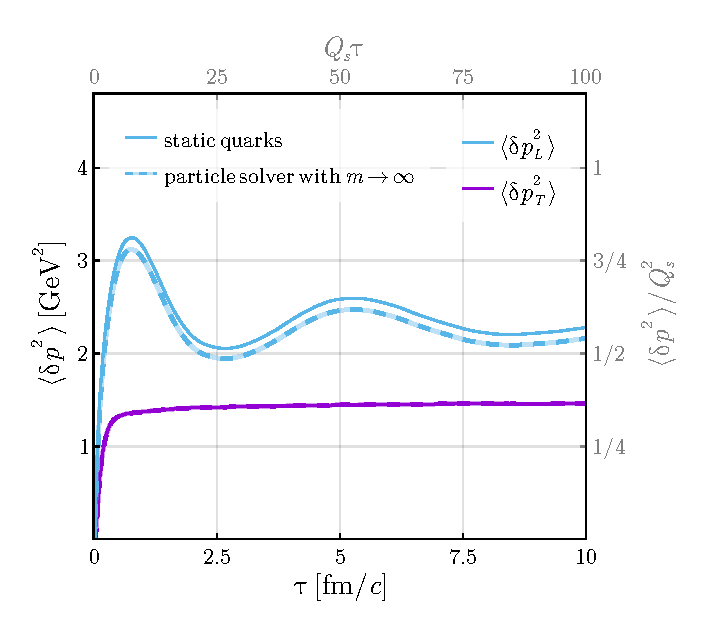
\includegraphics[width=0.75\textwidth]{images/wong_kappa.pdf}
        \end{figure}
        \column{.02\textwidth}
        \column{.5\textwidth}
        % \vspace{0.2cm}
        \begin{center}
            \setbeamertemplate{itemize item}{\raisebox{0.1em}{\scalebox{0.5}{${\color{lightgray}\blacktriangleright}$}}}
            {\Large\color{palteal} Momentum broadening $\langle \delta p^2\rangle$\\[5pt]
            Transport coefficients $\kappa$, $\hat{q}$  \\[10pt]}
            \footnotesize
                \begin{itemize}
                    \item {\color{lightgray}SU(3) glasma, longitudinal expansion}
                    \item {\color{lightgray}Numerical {\bfseries Wong's equations}}
                    \item {\color{lightgray}Colored-particle-in-cell solver}
                    \item {\color{lightgray}Comparison with {\bfseries field correlators}}
                \end{itemize}
                % {\footnotesize\color{lightgray}\texttt{Ballistic diffusion of heavy quarks in \\ the early stage of relativistic heavy \\ ion collisions at RHIC and LHC}}
        \end{center}
        \column{.02\textwidth}
    \end{columns}
    \blfootnote{\scriptsize DA, Băran, Greco, Ipp, Müller, Ruggieri \href{https://arxiv.org/abs/2303.05599}{\color{palgold}\texttt{[2303.05599]}$^\text{\scalebox{0.9}{\faExternalLink}}$}}
\end{frame}



%%%%%%%%%%%%%%%%%%%%%%%%%%%%%%%%%%%%%%%%%
%%%%%%%%%%%%%%%%% SLIDE %%%%%%%%%%%%%%%%%
%%%%%%%%%%%%%%%%%%%%%%%%%%%%%%%%%%%%%%%%%

\begin{frame}[t,noframenumbering]
    \frametitle{Literature timeline}
    \begin{center}
        \begin{tikzpicture}[xscale=1]
            \draw[line width=0.7mm,-latex,palteal!20] (-0.2,0) -- (6.5+0.2,0);
            \foreach \X [evaluate=\X as \Y using int(\X-2019),count=\Z] in {2020, 2021, 2023}
            {
            \draw[highlight on=<0>] (\Y,0) circle[radius=3pt];
            \node[anchor=south,highlight on=<0>,fill=white,rotate=45,anchor=south
            west,inner sep=0pt] at (\Y,0.2) {\X};
            }
            \foreach \X [evaluate=\X as \Y using int(\X-2019),count=\Z] in {2024}
            {
            \draw[highlight on=<\Z>] (\Y,0) circle[radius=3pt];
            \node[anchor=south,highlight on=<\Z>,fill=white,rotate=45,anchor=south
            west,inner sep=0pt] at (\Y,0.2) {\bfseries\X};
            }
        \end{tikzpicture}
    \end{center}
    \vspace{-10pt}
    \begin{columns}[onlytextwidth,t]
        \column{.02\textwidth}
       \column{.44\textwidth}
       \vspace{-13pt}
       \begin{figure}
            \centering
            \captionsetup{justification=centering}
            \caption{\texttt{Heavy-quark diffusion in\\ 2+1D and Glasma-like plasmas}}
            \vspace{-5pt}
            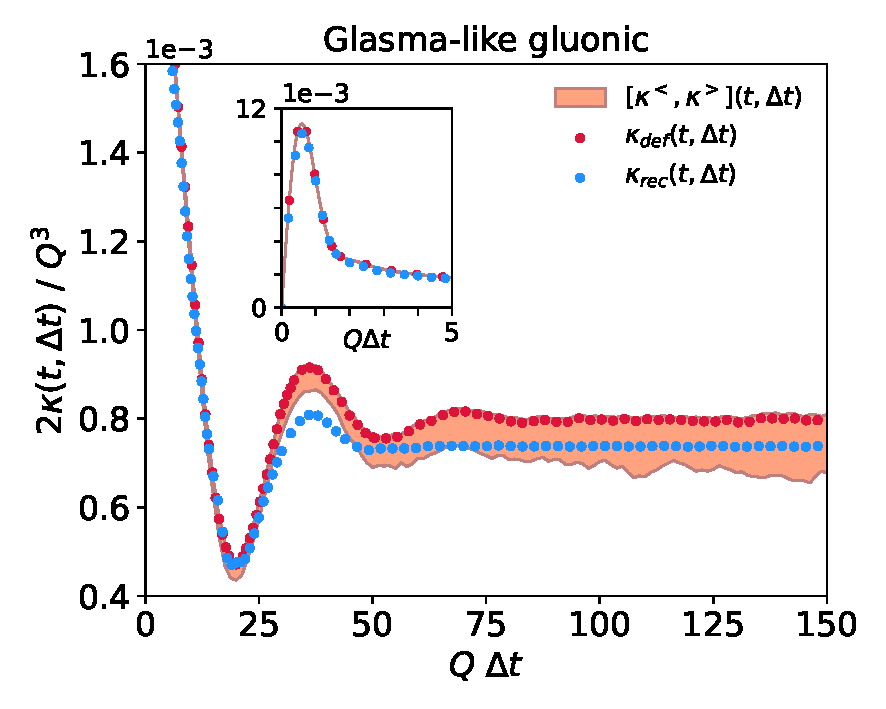
\includegraphics[width=0.75\textwidth]{images/2Dsc_g_SR_Qt500.pdf}
        \end{figure}
        \column{.02\textwidth}
        \column{.5\textwidth}
        % \vspace{0.2cm}
        \begin{center}
            \setbeamertemplate{itemize item}{\raisebox{0.1em}{\scalebox{0.5}{${\color{lightgray}\blacktriangleright}$}}}
            {\Large\color{palteal} Transport coefficient $\kappa$ \\[10pt]}
            \footnotesize
                \begin{itemize}
                    \item {\color{lightgray}Glasma-like classical gluon fields}
                    \item {\color{lightgray}Numerical lattice $\boldsymbol{\langle EE\rangle}$ {\bfseries  correlator}}
                    \item {\color{lightgray}Non-perturbative gluonic excitations}
                    \item {\color{lightgray}Explain the {\bfseries peak in $\boldsymbol{\kappa}$} from glasma}
                \end{itemize}
                % {\footnotesize\color{lightgray}\texttt{Ballistic diffusion of heavy quarks in \\ the early stage of relativistic heavy \\ ion collisions at RHIC and LHC}}
        \end{center}
        \column{.02\textwidth}
    \end{columns}
    \blfootnote{\scriptsize Backfried, Boguslavski, Hotzy \href{https://arxiv.org/abs/2408.12646}{\color{palgold}\texttt{[2408.12646]}$^\text{\scalebox{0.9}{\faExternalLink}}$}}
\end{frame}


%%%%%%%%%%%%%%%%%%%%%%%%%%%%%%%%%%%%%%%%%
%%%%%%%%%%%%%%%%% SLIDE %%%%%%%%%%%%%%%%%
%%%%%%%%%%%%%%%%%%%%%%%%%%%%%%%%%%%%%%%%%

\begin{frame}
    \frametitle{Jets in glasma}
    % \framesubtitle{Momentum broadening, transport coefficient, anisotropy}
    \begin{center}
        \begin{figure}
            \centering
            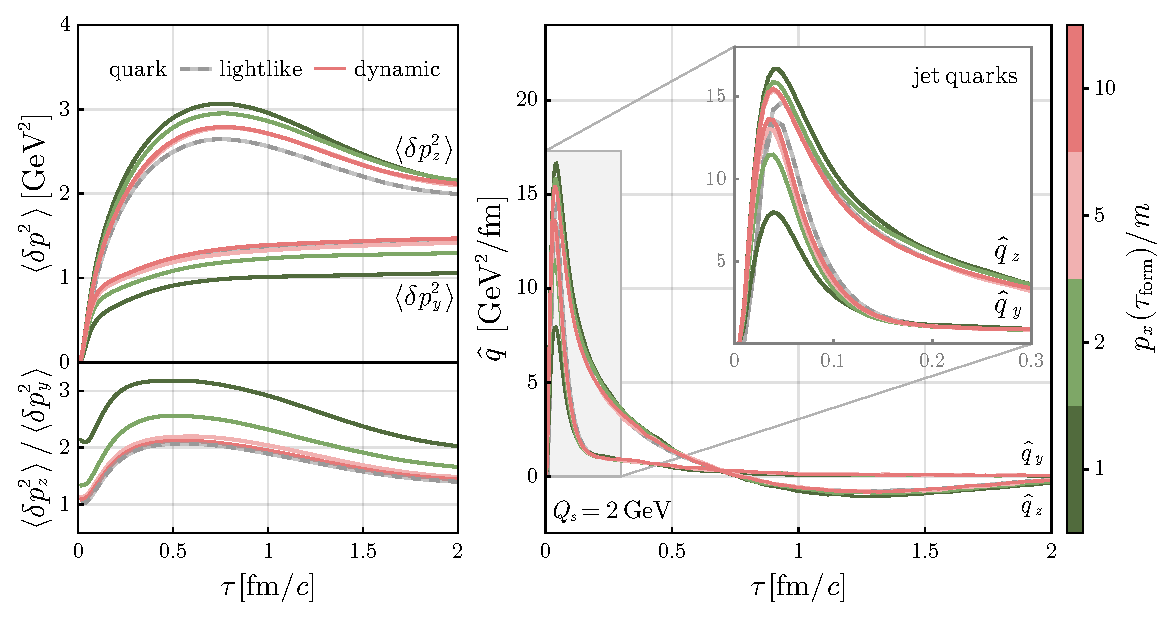
\includegraphics[width=0.85\textwidth]{images/hp23_mom_broad_qhat_anis_wong_vs_qhat.pdf}
        \end{figure}
    \end{center}
    \vspace{-20pt}
    \blfootnote{\scriptsize DA, Băran, Greco, Ipp, Müller, Ruggieri  \href{https://arxiv.org/abs/2307.07999}{{\color{custompink}\texttt{[2307.07999]}$^\text{\scalebox{0.9}{\faExternalLink}}$}}}
\end{frame}

%%%%%%%%%%%%%%%%%%%%%%%%%%%%%%%%%%%%%%%%%
%%%%%%%%%%%%%%%%% SLIDE %%%%%%%%%%%%%%%%%
%%%%%%%%%%%%%%%%%%%%%%%%%%%%%%%%%%%%%%%%%

\begin{frame}[noframenumbering]
    \frametitle{Jets in glasma}
    % \framesubtitle{Momentum broadening, transport coefficient, anisotropy}
    \begin{center}
        \begin{tikzpicture}
            \node[anchor=south west,inner sep=0] at (0,0) {\includegraphics[width=0.85\textwidth]{images/hp23_mom_broad_qhat_anis_wong_vs_qhat.pdf}};
            % \draw<1>[white, fill=white, fill opacity=0.9] (4.3,0.85) rectangle (5.4,5.5);
            \draw<1>[white,fill=white,fill opacity=0.9] (5.2,0.2) rectangle (13.0,6.8) node[opacity=1.0, pos=0.5, rotate=0, anchor=center, xshift=0.0 ,text width=7cm,align=center] {
                \begin{itemize}\itemsep0em 
                    \setbeamertemplate{itemize item}{\raisebox{0.2em}{\scalebox{0.7}{${\color{custompink}\blacktriangleright}$}}} 
                    \item \large {\color{custompink}Rapid increase in $\langle \delta p^2\rangle$ at early $\delta\tau$}\\[10pt]
                    \setbeamertemplate{itemize item}{\raisebox{0.2em}{\scalebox{0.7}{${\color{lightgray}\blacktriangleright}$}}} 
                    \item Different $\langle \delta p^2\rangle$ behavior at late $\delta\tau$
                        \begin{itemize}\itemsep0em 
                            \setbeamertemplate{itemize items}{\raisebox{0.1em}{\scalebox{0.6}{${\color{lightgray}\blacktriangleright}$}}} 
                            \item \color{lightgray}\footnotesize Transverse $\langle \delta p^2_y\rangle$ saturates
                            \item \color{lightgray}\footnotesize Longitudinal $\langle \delta p^2_z\rangle$ decreases\\[10pt]
                        \end{itemize}
                    \item \large Eikonal $\approx$ dynamic with large $p^x$ \\[10pt]
                        % \begin{itemize}\itemsep0em 
                        %     \setbeamertemplate{itemize items}{\raisebox{0.1em}{\scalebox{0.6}{${\color{lightgray}\blacktriangleright}$}}} 
                        %     \item \color{lightgray}\footnotesize Transverse $\langle \delta p^2_y\rangle$ increases with $p^x$
                        %     \item \color{lightgray}\footnotesize Longitudinal $\langle \delta p^2_z\rangle$ descreses with $p^x$\\[10pt]
                        % \end{itemize}
                    \item \large Anisotropic $\langle \delta p^2_z\rangle>\langle \delta p^2_y\rangle$ 
                    \begin{itemize}\itemsep0em 
                        \setbeamertemplate{itemize items}{\raisebox{0.1em}{\scalebox{0.6}{${\color{lightgray}\blacktriangleright}$}}} 
                        \item \color{lightgray}More anisotropic for small $p^x$
                    \end{itemize}
                \end{itemize}
                };
        \end{tikzpicture}
    \end{center}
    \vspace{-20pt}
    \blfootnote{\scriptsize DA, Băran, Greco, Ipp, Müller, Ruggieri  \href{https://arxiv.org/abs/2307.07999}{{\color{custompink}\texttt{[2307.07999]}$^\text{\scalebox{0.9}{\faExternalLink}}$}}}
\end{frame}


%%%%%%%%%%%%%%%%%%%%%%%%%%%%%%%%%%%%%%%%%
%%%%%%%%%%%%%%%%% SLIDE %%%%%%%%%%%%%%%%%
%%%%%%%%%%%%%%%%%%%%%%%%%%%%%%%%%%%%%%%%%

\begin{frame}[noframenumbering]
    \frametitle{Jets in glasma}
    % \framesubtitle{Momentum broadening, transport coefficient, anisotropy}
    \begin{center}
        \begin{tikzpicture}
            \hspace{-15pt}\node[anchor=south west,inner sep=0] at (0,0) {\includegraphics[width=0.85\textwidth]{images/hp23_mom_broad_qhat_anis_wong_vs_qhat.pdf}};
            % \draw<1>[white, fill=white, fill opacity=0.9] (4.3,0.85) rectangle (5.4,5.5);
            \draw<1>[white,fill=white,fill opacity=0.9] (0.0,0.2) rectangle (5.2,6.8) node[opacity=1.0, pos=0.5, rotate=0, anchor=center, xshift=0.0 ,text width=5.5cm,align=center] {tg
                \begin{itemize}\itemsep0em 
                    \setbeamertemplate{itemize item}{\raisebox{0.2em}{\scalebox{0.7}{${\color{custompink}\blacktriangleright}$}}} 
                    \item \large {\color{custompink} Large $\hat{q}$ peak at early $\delta\tau$}\\[10pt]
                    \setbeamertemplate{itemize item}{\raisebox{0.2em}{\scalebox{0.7}{${\color{lightgray}\blacktriangleright}$}}} 
                    \item Behavior of $\hat{q}$ at late $\delta\tau$
                        \begin{itemize}\itemsep0em 
                            \setbeamertemplate{itemize items}{\raisebox{0.1em}{\scalebox{0.6}{${\color{lightgray}\blacktriangleright}$}}} 
                            \item \color{lightgray}\footnotesize Transverse $\hat{q}_y\approx 0$
                            \item \color{lightgray}\footnotesize Longitudinal $\hat{q}_z<0$\\[10pt]
                        \end{itemize}
                    \item \large Anisotropic $\hat{q}_z\neq\hat{q}_y$ 
                    
                \end{itemize}
                };
        \end{tikzpicture}
    \end{center}
    \vspace{-20pt}
    \blfootnote{\scriptsize DA, Băran, Greco, Ipp, Müller, Ruggieri  \href{https://arxiv.org/abs/2307.07999}{{\color{custompink}\texttt{[2307.07999]}$^\text{\scalebox{0.9}{\faExternalLink}}$}}}
\end{frame}

    

%%%%%%%%%%%%%%%%%%%%%%%%%%%%%%%%%%%%%%%%%
%%%%%%%%%%%%%%%%% SLIDE %%%%%%%%%%%%%%%%%
%%%%%%%%%%%%%%%%%%%%%%%%%%%%%%%%%%%%%%%%%

\begin{frame}
    \frametitle{Heavy quarks in glasma}
    % \framesubtitle{Momentum broadening, transport coefficient, anisotropy}
    \begin{center}
        \begin{figure}
            \centering
            \includegraphics[width=0.85\textwidth]{images/hp23_mom_broad_kappa_anis_wong_vs_kappa.pdf}
        \end{figure}
    \end{center}
    \vspace{-20pt}
    \blfootnote{\scriptsize DA, Băran, Greco, Ipp, Müller, Ruggieri  \href{https://arxiv.org/abs/2307.07999}{{\color{Mahogany}\texttt{[2307.07999]}$^\text{\scalebox{0.9}{\faExternalLink}}$}}}
\end{frame}

%%%%%%%%%%%%%%%%%%%%%%%%%%%%%%%%%%%%%%%%%
%%%%%%%%%%%%%%%%% SLIDE %%%%%%%%%%%%%%%%%
%%%%%%%%%%%%%%%%%%%%%%%%%%%%%%%%%%%%%%%%%

\begin{frame}[noframenumbering]
    \frametitle{Heavy quarks in glasma}
    % \framesubtitle{Momentum broadening, transport coefficient, anisotropy}
    \begin{center}
        \begin{tikzpicture}
            \node[anchor=south west,inner sep=0] at (0,0) {\includegraphics[width=0.85\textwidth]{images/hp23_mom_broad_kappa_anis_wong_vs_kappa.pdf}};
            % \draw<1>[white, fill=white, fill opacity=0.9] (4.3,0.85) rectangle (5.4,5.5);
            \draw<1>[white,fill=white,fill opacity=0.9] (5.2,0.2) rectangle (13.0,6.8) node[opacity=1.0, pos=0.5, rotate=0, anchor=center, xshift=0.0 ,text width=7cm,align=center] {
                \begin{itemize}\itemsep0em 
                    \setbeamertemplate{itemize item}{\raisebox{0.2em}{\scalebox{0.7}{${\color{Mahogany}\blacktriangleright}$}}} 
                    \item \large {\color{Mahogany}Rapid increase in $\langle \delta p^2\rangle$ at early $\delta\tau$}\\[10pt]
                    \setbeamertemplate{itemize item}{\raisebox{0.2em}{\scalebox{0.7}{${\color{lightgray}\blacktriangleright}$}}} 
                    \item Different $\langle \delta p^2\rangle$ behavior at late $\delta\tau$
                        \begin{itemize}\itemsep0em 
                            \setbeamertemplate{itemize items}{\raisebox{0.1em}{\scalebox{0.6}{${\color{lightgray}\blacktriangleright}$}}} 
                            \item \color{lightgray}\footnotesize Transverse $\langle \delta p^2_T\rangle$ saturates
                            \item \color{lightgray}\footnotesize Longitudinal $\langle \delta p^2_L\rangle$ oscilates\\[10pt]
                        \end{itemize}
                    \item \large Static $\neq$ dynamic with $p_T(\tau_\mathrm{form})$ \\[10pt]
                        % \begin{itemize}\itemsep0em 
                        %     \setbeamertemplate{itemize items}{\raisebox{0.1em}{\scalebox{0.6}{${\color{lightgray}\blacktriangleright}$}}} 
                        %     \item \color{lightgray}\footnotesize Transverse $\langle \delta p^2_T\rangle$ increases with $p_T$
                        %     \item \color{lightgray}\footnotesize Longitudinal $\langle \delta p^2_L\rangle$ descreses with $p_T$\\[10pt]
                        % \end{itemize}
                    \item \large Anisotropic $\langle \delta p^2_L\rangle>\langle \delta p^2_T\rangle$ 
                    \begin{itemize}\itemsep0em 
                        \setbeamertemplate{itemize items}{\raisebox{0.1em}{\scalebox{0.6}{${\color{lightgray}\blacktriangleright}$}}} 
                        \item \color{lightgray}More anisotropic for small $p_T$
                    \end{itemize}
                \end{itemize}
                };
        \end{tikzpicture}
    \end{center}
    \vspace{-20pt}
    \blfootnote{\scriptsize DA, Băran, Greco, Ipp, Müller, Ruggieri  \href{https://arxiv.org/abs/2307.07999}{{\color{Mahogany}\texttt{[2307.07999]}$^\text{\scalebox{0.9}{\faExternalLink}}$}}}
\end{frame}


%%%%%%%%%%%%%%%%%%%%%%%%%%%%%%%%%%%%%%%%%
%%%%%%%%%%%%%%%%% SLIDE %%%%%%%%%%%%%%%%%
%%%%%%%%%%%%%%%%%%%%%%%%%%%%%%%%%%%%%%%%%

\begin{frame}[noframenumbering]
    \frametitle{Heavy quarks in glasma}
    % \framesubtitle{Momentum broadening, transport coefficient, anisotropy}
    \begin{center}
        \begin{tikzpicture}
            \hspace{-15pt}\node[anchor=south west,inner sep=0] at (0,0) {\includegraphics[width=0.85\textwidth]{images/hp23_mom_broad_kappa_anis_wong_vs_kappa.pdf}};
            % \draw<1>[white, fill=white, fill opacity=0.9] (4.3,0.85) rectangle (5.4,5.5);
            \draw<1>[white,fill=white,fill opacity=0.9] (0.0,0.2) rectangle (5.2,6.8) node[opacity=1.0, pos=0.5, rotate=0, anchor=center, xshift=0.0 ,text width=5.5cm,align=center] {tg
                \begin{itemize}\itemsep0em 
                    \setbeamertemplate{itemize item}{\raisebox{0.2em}{\scalebox{0.7}{${\color{Mahogany}\blacktriangleright}$}}} 
                    \item \large {\color{Mahogany} Large $\kappa$ peak at early $\delta\tau$}\\[10pt]
                    \setbeamertemplate{itemize item}{\raisebox{0.2em}{\scalebox{0.7}{${\color{lightgray}\blacktriangleright}$}}} 
                    \item Behavior of $\kappa$ at late $\delta\tau$
                        \begin{itemize}\itemsep0em 
                            \setbeamertemplate{itemize items}{\raisebox{0.1em}{\scalebox{0.6}{${\color{lightgray}\blacktriangleright}$}}} 
                            \item \color{lightgray}\footnotesize Transverse $\kappa_T\approx 0$
                            \item \color{lightgray}\footnotesize Longitudinal $\kappa_L<0$\\[10pt]
                        \end{itemize}
                    \item \large Anisotropic $\kappa_L\neq\kappa_T$ 
                    
                \end{itemize}
                };
        \end{tikzpicture}
    \end{center}
    \vspace{-20pt}
    \blfootnote{\scriptsize DA, Băran, Greco, Ipp, Müller, Ruggieri  \href{https://arxiv.org/abs/2307.07999}{{\color{Mahogany}\texttt{[2307.07999]}$^\text{\scalebox{0.9}{\faExternalLink}}$}}}
\end{frame}





%%%%%%%%%%%%%%%%%%%%%%%%%%%%%%%%%%%%%%%%%
%%%%%%%%%%%%%%%%% SLIDE %%%%%%%%%%%%%%%%%
%%%%%%%%%%%%%%%%%%%%%%%%%%%%%%%%%%%%%%%%%


\begin{frame}
    \frametitle{Large $\hat{q}$ in glasma}
    \framesubtitle{Compatible with EKT}
    \vspace{-0.4cm}
    \begin{columns}[onlytextwidth,t]
    \column{.5\textwidth}
        \begin{figure}[!hbt]
            \centering
            \captionsetup{justification=centering}
            \caption{Schematic evolution of $\hat{q}$}\vspace{-0.3cm}
            \includegraphics[width=0.8\columnwidth]{images/qhat_schematic_evolution.pdf}\vspace{-0.3cm}
            % \caption{\scriptsize\itshape Figure from \href{https://arxiv.org/abs/2303.12595}{\color{ForestGreen}[2303.12595]}}
        \end{figure}
    \column{.5\textwidth}
        \begin{figure}[!hbt]
            \centering
            \captionsetup{justification=centering}
            \caption{{\color{ForestGreen}Kinetic theory} connects the large $\hat{q}$ in {\color{Dandelion}Glasma}\\ to subsequent {\color{Periwinkle}hydrodynamics}}\vspace{-0.2cm}
            \includegraphics[width=0.8\columnwidth]{images/2023-03-07-16-41-35_qhat_appetizer_glasma_comparison_493.pdf}
        \end{figure}
    \end{columns}   

    \blfootnote{\scriptsize Boguslavski, Kurkela, Lappi, Lindenbauer, Peuron \href{https://arxiv.org/abs/2303.12595}{{\color{ForestGreen}\texttt{[2303.12595]}$^\text{\scalebox{0.9}{\faExternalLink}}$}}, \href{https://arxiv.org/abs/2312.00447}{{\color{ForestGreen}\texttt{[2312.00447]}$^\text{\scalebox{0.9}{\faExternalLink}}$}}}
    \begin{tikzpicture}[overlay, remember picture]
        \node[anchor=north west] 
        at ([xshift=0.05cm,yshift=-0.05cm]current page.north west) {\begin{talkbox}\scriptsize{\color{destacado}Lindenbauer$\hspace{1pt}^\text{\scalebox{0.9}{\faComment}}$} {\itshape Mon 15:15$\hspace{1pt}^\text{\scalebox{0.9}{\faClockO}}$} \end{talkbox}};
    \end{tikzpicture}
    \begin{tikzpicture}[overlay, remember picture]
        \node[anchor=north west] 
        at ([xshift=0.05cm,yshift=-0.48cm]current page.north west) {\begin{talkbox}\scriptsize Jets in EKT \end{talkbox}};
    \end{tikzpicture}
    \begin{tikzpicture}[overlay, remember picture]
        \node[anchor=north west] 
        at ([xshift=0.05cm,yshift=-1.05cm]current page.north west) {\begin{talkbox}\scriptsize{\color{destacado}Zhou$\hspace{1pt}^\text{\scalebox{0.9}{\faComment}}$} {\itshape Tue 12:30$\hspace{1pt}^\text{\scalebox{0.9}{\faClockO}}$} \end{talkbox}};
    \end{tikzpicture}
    \begin{tikzpicture}[overlay, remember picture]
        \node[anchor=north west] 
        at ([xshift=0.05cm,yshift=-1.48cm]current page.north west) {\begin{talkbox}\scriptsize{Minijets in EKT} \end{talkbox}};
    \end{tikzpicture}
\end{frame}

%%%%%%%%%%%%%%%%%%%%%%%%%%%%%%%%%%%%%%%%%
%%%%%%%%%%%%%%%%% SLIDE %%%%%%%%%%%%%%%%%
%%%%%%%%%%%%%%%%%%%%%%%%%%%%%%%%%%%%%%%%%

\begin{frame}[noframenumbering]
    \frametitle{The ``creation'' of $\hat{q}$}
    \framesubtitle{Glasma and EKT initial stages}
    \vspace{-0.4cm}
    \begin{columns}[onlytextwidth,t]
    \column{.5\textwidth}
        \begin{figure}[!hbt]
            \centering
            \captionsetup{justification=centering}
            \caption{Schematic evolution of $\hat{q}$}\vspace{-0.3cm}
            \includegraphics[width=0.78\columnwidth]{images/qhat_schematic_evolution.pdf}\vspace{-0.3cm}
            % \caption{\scriptsize\itshape Figure from \href{https://arxiv.org/abs/2303.12595}{\color{ForestGreen}[2303.12595]}}
        \end{figure}
    \column{.5\textwidth}
        \begin{figure}[!hbt]
            \centering
            \captionsetup{justification=centering}
            \caption{{\color{ForestGreen}Kinetic theory} connects the large $\hat{q}$ in {\color{Dandelion}Glasma}\\ to subsequent {\color{Periwinkle}hydrodynamics}}\vspace{-0.2cm}
            \includegraphics[width=0.8\columnwidth]{images/qhat_glasma_ekt.png}
        \end{figure}
    \end{columns}   
    \blfootnote{\scriptsize Boguslavski, Kurkela, Lappi, Lindenbauer, Peuron \href{https://arxiv.org/abs/2303.12595}{{\color{ForestGreen}\texttt{[2303.12595]}$^\text{\scalebox{0.9}{\faExternalLink}}$}}, \href{https://arxiv.org/abs/2312.00447}{{\color{ForestGreen}\texttt{[2312.00447]}$^\text{\scalebox{0.9}{\faExternalLink}}$}}}
    % \begin{tikzpicture}[overlay, remember picture]
    %     \node[anchor=north west] 
    %     at ([xshift=0.05cm,yshift=-0.05cm]current page.north west) {\begin{talkbox}\scriptsize{\color{destacado}Lindenbauer$\hspace{1pt}^\text{\scalebox{0.9}{\faComment}}$} {\itshape Mon 15:15$\hspace{1pt}^\text{\scalebox{0.9}{\faClockO}}$} \end{talkbox}};
    % \end{tikzpicture}
    % \begin{tikzpicture}[overlay, remember picture]
    %     \node[anchor=north west] 
    %     at ([xshift=0.05cm,yshift=-0.48cm]current page.north west) {\begin{talkbox}\scriptsize Jets in EKT \end{talkbox}};
    % \end{tikzpicture}
\end{frame}




%%%%%%%%%%%%%%%%%%%%%%%%%%%%%%%%%%%%%%%%%
%%%%%%%%%%%%%%%%% SLIDE %%%%%%%%%%%%%%%%%
%%%%%%%%%%%%%%%%%%%%%%%%%%%%%%%%%%%%%%%%%


\begin{frame}
    \frametitle{Large $\kappa$ in glasma}
    \framesubtitle{Not yet compatible with EKT}
    \vspace{-0.4cm}
    \begin{columns}[onlytextwidth,t]
    \column{.5\textwidth}
        \begin{figure}[!hbt]
            \centering
            \captionsetup{justification=centering}
            \caption{Schematic evolution of $\kappa$}\vspace{-0.3cm}
            \includegraphics[width=0.8\columnwidth]{images/kappa_schematic.png}\vspace{-0.3cm}
            % \caption{\scriptsize\itshape Figure from \href{https://arxiv.org/abs/2303.12595}{\color{ForestGreen}[2303.12595]}}
        \end{figure}
    \column{.5\textwidth}
        \begin{figure}[!hbt]
            \centering
            \captionsetup{justification=centering}
            \caption{{\color{ForestGreen}Kinetic theory} doesn't smoothly connect the large $\kappa$\\ in {\color{Dandelion}Glasma} to subsequent {\color{Periwinkle}hydrodynamics}}\vspace{-0.2cm}
            \includegraphics[width=0.8\columnwidth]{images/KappaGlasmaVsEKTvsLatticev2.pdf}
        \end{figure}
    \end{columns}   

    \blfootnote{\scriptsize Boguslavski, Kurkela, Lappi, Lindenbauer, Peuron \href{https://arxiv.org/abs/2303.12520}{{\color{ForestGreen}\texttt{[2303.12520]}$^\text{\scalebox{0.9}{\faExternalLink}}$}}}
    \begin{tikzpicture}[overlay, remember picture]
        \node[anchor=north west] 
        at ([xshift=0.05cm,yshift=-0.05cm]current page.north west) {\begin{talkbox}\scriptsize{\color{destacado}Lindenbauer$\hspace{1pt}^\text{\scalebox{0.9}{\faComment}}$} {\itshape Mon 15:15$\hspace{1pt}^\text{\scalebox{0.9}{\faClockO}}$} \end{talkbox}};
    \end{tikzpicture}
    \begin{tikzpicture}[overlay, remember picture]
        \node[anchor=north west] 
        at ([xshift=0.05cm,yshift=-0.48cm]current page.north west) {\begin{talkbox}\scriptsize HQs in EKT \end{talkbox}};
    \end{tikzpicture}
    \begin{tikzpicture}[overlay, remember picture]
        \node[anchor=north west] 
        at ([xshift=0.05cm,yshift=-1.05cm]current page.north west) {\begin{talkbox}\scriptsize{\color{destacado}Du$\hspace{1pt}^\text{\scalebox{0.9}{\faComment}}$} {\itshape Fri 11:00$\hspace{1pt}^\text{\scalebox{0.9}{\faClockO}}$} \end{talkbox}};
    \end{tikzpicture}
    \begin{tikzpicture}[overlay, remember picture]
        \node[anchor=north west] 
        at ([xshift=0.05cm,yshift=-1.48cm]current page.north west) {\begin{talkbox}\scriptsize{HQ diffusion in EKT} \end{talkbox}};
    \end{tikzpicture}
\end{frame}

%%%%%%%%%%%%%%%%%%%%%%%%%%%%%%%%%%%%%%%%%
%%%%%%%%%%%%%%%%% SLIDE %%%%%%%%%%%%%%%%%
%%%%%%%%%%%%%%%%%%%%%%%%%%%%%%%%%%%%%%%%%

\begin{frame}[noframenumbering]
    \frametitle{Can we ``create'' $\kappa$?}
    \framesubtitle{Glasma and EKT initial stages}
    \vspace{-0.4cm}
    \begin{columns}[onlytextwidth,t]
    \column{.5\textwidth}
        \begin{figure}[!hbt]
            \centering
            \captionsetup{justification=centering}
            \caption{Schematic evolution of $\kappa$}\vspace{-0.3cm}
            \includegraphics[width=0.78\columnwidth]{images/kappa_schematic.png}\vspace{-0.3cm}
            % \caption{\scriptsize\itshape Figure from \href{https://arxiv.org/abs/2303.12595}{\color{ForestGreen}[2303.12595]}}
        \end{figure}
    \column{.5\textwidth}
        \begin{figure}[!hbt]
            \centering
            \captionsetup{justification=centering}
            \caption{{\color{ForestGreen}Kinetic theory} doesn't smoothly connect the large $\kappa$\\ in {\color{Dandelion}Glasma} to subsequent {\color{Periwinkle}hydrodynamics}}\vspace{-0.2cm}
            \includegraphics[width=0.9\columnwidth]{images/kappa_glasma_ekt.png}
        \end{figure}
    \end{columns}   
    \blfootnote{\scriptsize Boguslavski, Kurkela, Lappi, Lindenbauer, Peuron \href{https://arxiv.org/abs/2303.12520}{{\color{ForestGreen}\texttt{[2303.12520]}$^\text{\scalebox{0.9}{\faExternalLink}}$}}}
    % \begin{tikzpicture}[overlay, remember picture]
    %     \node[anchor=north west] 
    %     at ([xshift=0.05cm,yshift=-0.05cm]current page.north west) {\begin{talkbox}\scriptsize{\color{destacado}Lindenbauer$\hspace{1pt}^\text{\scalebox{0.9}{\faComment}}$} {\itshape Mon 15:15$\hspace{1pt}^\text{\scalebox{0.9}{\faClockO}}$} \end{talkbox}};
    % \end{tikzpicture}
    % \begin{tikzpicture}[overlay, remember picture]
    %     \node[anchor=north west] 
    %     at ([xshift=0.05cm,yshift=-0.48cm]current page.north west) {\begin{talkbox}\scriptsize HQs in EKT \end{talkbox}};
    % \end{tikzpicture}
\end{frame}



%%%%%%%%%%%%%%%%%%%%%%%%%%%%%%%%%%%%%%%%%
%%%%%%%%%%%%%% SUBSECTION %%%%%%%%%%%%%%%
%%%%%%%%%%%%%%%%%%%%%%%%%%%%%%%%%%%%%%%%%

\subsection{Observables}

\setbeamertemplate{background}{
\tikz[overlay,remember picture] \node[opacity=0.15, at=(current page.center)] {
   \includegraphics[height=0.8\paperheight]{images/Cdetadphi_3D_toy_charm_pT_1_tau_0.1_crop.png}};
}
\begin{frame}[plain,noframenumbering]{}
    \begin{center}
        \vspace{1cm}
        {\large\color{normal}How to probe pre-equilibrium}\\[0.3cm]
        {\huge\color{destacado}Sensitivity to early stages}\\[0.4cm]
        {\large\textit{Candidates: $R_{AA}$, $v_2$, others...}}
    \end{center}
    \begin{tikzpicture}[overlay, remember picture]
        \node[anchor=north west] 
        at ([xshift=0.05cm,yshift=-0.05cm]current page.north west) {\begin{talkbox}\scriptsize{\color{destacado}Greco$\hspace{1pt}^\text{\scalebox{0.9}{\faComment}}$} {\itshape Tue 15:15$\hspace{1pt}^\text{\scalebox{0.9}{\faClockO}}$} \end{talkbox}};
    \end{tikzpicture}
    \begin{tikzpicture}[overlay, remember picture]
        \node[anchor=north west] 
        at ([xshift=0.05cm,yshift=-0.48cm]current page.north west) {\begin{talkbox}\scriptsize{HQs in glasma pheno} \end{talkbox}};
    \end{tikzpicture}
\end{frame}
\setbeamertemplate{background}{}


%%%%%%%%%%%%%%%%%%%%%%%%%%%%%%%%%%%%%%%%%
%%%%%%%%%%%%%%%%% SLIDE %%%%%%%%%%%%%%%%%
%%%%%%%%%%%%%%%%%%%%%%%%%%%%%%%%%%%%%%%%%

\begin{frame}[t]
    \frametitle{Literature timeline}
    \begin{center}
        \begin{tikzpicture}[xscale=1]
            \draw[line width=0.7mm,-latex,palteal!20] (-0.2,0) -- (8.5+0.2,0);
            \foreach \X [evaluate=\X as \Y using int(\X-2017),count=\Z] in {2019, 2022, 2024}
            {
            \draw[highlight on=<0>] (\Y,0) circle[radius=3pt];
            \node[anchor=south,highlight on=<0>,fill=white,rotate=45,anchor=south
            west,inner sep=0pt] at (\Y,0.2) {\X};
            }
            \foreach \X [evaluate=\X as \Y using int(\X-2017),count=\Z] in {2018}
            {
            \draw[highlight on=<\Z>] (\Y,0) circle[radius=3pt];
            \node[anchor=south,highlight on=<\Z>,fill=white,rotate=45,anchor=south
            west,inner sep=0pt] at (\Y,0.2) {\bfseries\X};
            }
        \end{tikzpicture}
    \end{center}
    \vspace{-10pt}
    \begin{columns}[onlytextwidth,t]
        \column{.02\textwidth}
       \column{.43\textwidth}
       \vspace{-13pt}
       \begin{figure}
            \centering
            \captionsetup{justification=centering}
            \caption{\texttt{The cathode tube effect}: \texttt{heavy \\ quarks probing the Glasma}}
            \vspace{-5pt}
            \includegraphics[width=0.8\textwidth]{images/pPb_RpPb_FRAGME_new_2_crop.pdf}
        \end{figure}
        \column{.02\textwidth}
        \column{.5\textwidth}
        % \vspace{0.2cm}
        \begin{center}
            \setbeamertemplate{itemize item}{\raisebox{0.1em}{\scalebox{0.5}{${\color{lightgray}\blacktriangleright}$}}}
            {\Large\color{palteal} $R_{pA}$ for D-mesons  \\[10pt]}
            \footnotesize
                \begin{itemize}
                    \item {\color{lightgray}SU(2) glasma, {\bfseries static box}}
                    \item {\color{lightgray}Numerical {\bfseries Wong's equations}}
                    \item {\color{lightgray}Proton $Q_s$ from {\bfseries hot spots} model}
                    \item {\color{lightgray}FONLL $p_T$-spetra + fragmentation $D_{c\rightarrow D}$}
                \end{itemize}
                % {\footnotesize\color{lightgray}\texttt{Ballistic diffusion of heavy quarks in \\ the early stage of relativistic heavy \\ ion collisions at RHIC and LHC}}
        \end{center}
        \column{.02\textwidth}
    \end{columns}
    \blfootnote{\scriptsize Ruggieri, Das \href{https://arxiv.org/abs/1805.09617}{\color{palgold}\texttt{[1805.09617]}$^\text{\scalebox{0.9}{\faExternalLink}}$}}
    \begin{tikzpicture}[overlay, remember picture]
        \node[anchor=north west] 
        at ([xshift=0.05cm,yshift=-0.05cm]current page.north west) {\begin{talkbox}\scriptsize{\color{destacado}Ruggieri$\hspace{1pt}^\text{\scalebox{0.9}{\faComment}}$} {\itshape Mon 11:00$\hspace{1pt}^\text{\scalebox{0.9}{\faClockO}}$} \end{talkbox}};
    \end{tikzpicture}
    \begin{tikzpicture}[overlay, remember picture]
        \node[anchor=north west] 
        at ([xshift=0.05cm,yshift=-0.48cm]current page.north west) {\begin{talkbox}\scriptsize{HQs in glasma $R_{pA}$} \end{talkbox}};
    \end{tikzpicture}
\end{frame}


%%%%%%%%%%%%%%%%%%%%%%%%%%%%%%%%%%%%%%%%%
%%%%%%%%%%%%%%%%% SLIDE %%%%%%%%%%%%%%%%%
%%%%%%%%%%%%%%%%%%%%%%%%%%%%%%%%%%%%%%%%%

\begin{frame}[t,noframenumbering]
    \frametitle{Literature timeline}
    \begin{center}
        \begin{tikzpicture}[xscale=1]
            \draw[line width=0.7mm,-latex,palteal!20] (-0.2,0) -- (8.5+0.2,0);
            \foreach \X [evaluate=\X as \Y using int(\X-2017),count=\Z] in {2018, 2022, 2024}
            {
            \draw[highlight on=<0>] (\Y,0) circle[radius=3pt];
            \node[anchor=south,highlight on=<0>,fill=white,rotate=45,anchor=south
            west,inner sep=0pt] at (\Y,0.2) {\X};
            }
            \foreach \X [evaluate=\X as \Y using int(\X-2017),count=\Z] in {2019}
            {
            \draw[highlight on=<\Z>] (\Y,0) circle[radius=3pt];
            \node[anchor=south,highlight on=<\Z>,fill=white,rotate=45,anchor=south
            west,inner sep=0pt] at (\Y,0.2) {\bfseries\X};
            }
        \end{tikzpicture}
    \end{center}
    \vspace{-10pt}
    \begin{columns}[onlytextwidth,t]
        \column{.02\textwidth}
       \column{.43\textwidth}
       \vspace{-13pt}
       \begin{figure}
            \centering
            \captionsetup{justification=centering}
            \caption{\texttt{Impact of Glasma on heavy quark \\ observables in AA collisions}}
            % \vspace{-5pt}
            \includegraphics[width=0.8\textwidth]{images/1-s2.0-S0370269319306550-gr003_lrg.jpg}
        \end{figure}
        \column{.02\textwidth}
        \column{.5\textwidth}
        % \vspace{0.2cm}
        \begin{center}
            \setbeamertemplate{itemize item}{\raisebox{0.1em}{\scalebox{0.5}{${\color{lightgray}\blacktriangleright}$}}}
            {\Large\color{palteal} Hybrid $R_{AA}$ and $v_2$ for D-mesons \\[10pt]}
            \footnotesize
                \begin{itemize}
                    \item {\color{lightgray}SU(2) glasma, {\bfseries static box}}
                    \item {\color{lightgray}Numerical {\bfseries Wong's equations}}
                    \item {\color{lightgray}Compared with Langevin with $\Gamma$ and $D$}
                    \item {\color{lightgray}Considering the glasma {\bfseries increases} $\boldsymbol{v_2}$}
                \end{itemize}
                % {\footnotesize\color{lightgray}\texttt{Ballistic diffusion of heavy quarks in \\ the early stage of relativistic heavy \\ ion collisions at RHIC and LHC}}
        \end{center}
        \column{.02\textwidth}
    \end{columns}
    \blfootnote{\scriptsize Sun, Coci, Das, Plumari, Ruggieri, Greco \href{https://arxiv.org/abs/1902.06254}{\color{palgold}\texttt{[1902.06254]}$^\text{\scalebox{0.9}{\faExternalLink}}$}}
    \begin{tikzpicture}[overlay, remember picture]
        \node[anchor=north west] 
        at ([xshift=0.05cm,yshift=-0.05cm]current page.north west) {\begin{talkbox}\scriptsize{\color{destacado}Greco$\hspace{1pt}^\text{\scalebox{0.9}{\faComment}}$} {\itshape Tue 15:15$\hspace{1pt}^\text{\scalebox{0.9}{\faClockO}}$} \end{talkbox}};
    \end{tikzpicture}
    \begin{tikzpicture}[overlay, remember picture]
        \node[anchor=north west] 
        at ([xshift=0.05cm,yshift=-0.48cm]current page.north west) {\begin{talkbox}\scriptsize{HQs in glasma $R_{AA}$} \end{talkbox}};
    \end{tikzpicture}
\end{frame}


%%%%%%%%%%%%%%%%%%%%%%%%%%%%%%%%%%%%%%%%%
%%%%%%%%%%%%%%%%% SLIDE %%%%%%%%%%%%%%%%%
%%%%%%%%%%%%%%%%%%%%%%%%%%%%%%%%%%%%%%%%%

\begin{frame}[t,noframenumbering]
    \frametitle{Literature timeline}
    \begin{center}
        \begin{tikzpicture}[xscale=1]
            \draw[line width=0.7mm,-latex,palteal!20] (-0.2,0) -- (8.5+0.2,0);
            \foreach \X [evaluate=\X as \Y using int(\X-2017),count=\Z] in {2018, 2022, 2024}
            {
            \draw[highlight on=<0>] (\Y,0) circle[radius=3pt];
            \node[anchor=south,highlight on=<0>,fill=white,rotate=45,anchor=south
            west,inner sep=0pt] at (\Y,0.2) {\X};
            }
            \foreach \X [evaluate=\X as \Y using int(\X-2017),count=\Z] in {2019}
            {
            \draw[highlight on=<\Z>] (\Y,0) circle[radius=3pt];
            \node[anchor=south,highlight on=<\Z>,fill=white,rotate=45,anchor=south
            west,inner sep=0pt] at (\Y,0.2) {\bfseries\X};
            }
        \end{tikzpicture}
    \end{center}
    \vspace{-10pt}
    \begin{columns}[onlytextwidth,t]
        \column{.02\textwidth}
       \column{.47\textwidth}
       \vspace{-13pt}
       \begin{figure}
            \centering
            \captionsetup{justification=centering}
            \caption{\texttt{Jet quenching as a probe \\ of the initial stages}}
            \vspace{-5pt}
            \includegraphics[width=\textwidth]{images/raa-vn-tauq_crop.pdf}
        \end{figure}
        \column{.02\textwidth}
        \column{.46\textwidth}
        % \vspace{0.2cm}
        \begin{center}
            \setbeamertemplate{itemize item}{\raisebox{0.1em}{\scalebox{0.5}{${\color{lightgray}\blacktriangleright}$}}}
            {\Large\color{palteal} $R_{AA}$ and $v_2$ for jets \\[10pt]}
            \footnotesize
                \begin{itemize}
                    \item {\color{lightgray}{\bfseries EKRT} initial condition, {\bfseries no glasma}}
                    \item {\color{lightgray}Relativistic boost-invariant hydrodynamics}
                    \item {\color{lightgray}Jet quenching using {\bfseries BDMPS-Z} formalism}
                    \item {\color{lightgray}Energy loss in suppressed in first $\sim 0.6\,\mathrm{fm/c}$}
                    \item {\color{lightgray}Initial stage energy loss affects $v_2$}
                \end{itemize}
                % {\footnotesize\color{lightgray}\texttt{Ballistic diffusion of heavy quarks in \\ the early stage of relativistic heavy \\ ion collisions at RHIC and LHC}}
        \end{center}
        \column{.02\textwidth}
    \end{columns}
    \blfootnote{\scriptsize Andres, Armesto, Niemi, Paatelainen, Salgado \href{https://arxiv.org/abs/1902.03231}{\color{palgold}\texttt{[1902.03231]}$^\text{\scalebox{0.9}{\faExternalLink}}$}}
\end{frame}


%%%%%%%%%%%%%%%%%%%%%%%%%%%%%%%%%%%%%%%%%
%%%%%%%%%%%%%%%%% SLIDE %%%%%%%%%%%%%%%%%
%%%%%%%%%%%%%%%%%%%%%%%%%%%%%%%%%%%%%%%%%

\begin{frame}[t,noframenumbering]
    \frametitle{Literature timeline}
    \begin{center}
        \begin{tikzpicture}[xscale=1]
            \draw[line width=0.7mm,-latex,palteal!20] (-0.2,0) -- (8.5+0.2,0);
            \foreach \X [evaluate=\X as \Y using int(\X-2017),count=\Z] in {2018, 2022, 2024}
            {
            \draw[highlight on=<0>] (\Y,0) circle[radius=3pt];
            \node[anchor=south,highlight on=<0>,fill=white,rotate=45,anchor=south
            west,inner sep=0pt] at (\Y,0.2) {\X};
            }
            \foreach \X [evaluate=\X as \Y using int(\X-2017),count=\Z] in {2019}
            {
            \draw[highlight on=<\Z>] (\Y,0) circle[radius=3pt];
            \node[anchor=south,highlight on=<\Z>,fill=white,rotate=45,anchor=south
            west,inner sep=0pt] at (\Y,0.2) {\bfseries\X};
            }
        \end{tikzpicture}
    \end{center}
    \vspace{-10pt}
    \begin{columns}[onlytextwidth,t]
        \column{.02\textwidth}
       \column{.47\textwidth}
       \vspace{-13pt}
       \begin{figure}
            \centering
            \captionsetup{justification=centering}
            \caption{\texttt{Exploring the initial stages with\\ high-$p_T$ $R_{AA}$ and $v_2$ theory and data}}
            \vspace{-5pt}
            \includegraphics[width=\textwidth]{images/InitialConditions_Fig2_Fig3_merge.pdf}
        \end{figure}
        \column{.02\textwidth}
        \column{.46\textwidth}
        % \vspace{0.2cm}
        \begin{center}
            \setbeamertemplate{itemize item}{\raisebox{0.1em}{\scalebox{0.5}{${\color{lightgray}\blacktriangleright}$}}}
            {\Large\color{palteal} $R_{AA}$ and $v_2$ for high-$p_T$ \\[10pt]}
            \footnotesize
                \begin{itemize}
                    \item {\color{lightgray}{\bfseries DREENA} framework for energy loss}
                    \item {\color{lightgray}Bjorken hydrodynamics for medium evolution}
                    \item {\color{lightgray}Radiative and collisional energy loss}
                    \item {\color{lightgray}Different {\bfseries initial $\boldsymbol{T}$ profiles}, {\bfseries no glasma}}
                    \item {\color{lightgray}No effect on $v_2$, {\bfseries only $\boldsymbol{R_{AA}}$ is affected}}
                \end{itemize}
                % {\footnotesize\color{lightgray}\texttt{Ballistic diffusion of heavy quarks in \\ the early stage of relativistic heavy \\ ion collisions at RHIC and LHC}}
        \end{center}
        \column{.02\textwidth}
    \end{columns}
    \blfootnote{\scriptsize Zigic, Ilic, Djordjevic, Djordjevic \href{https://arxiv.org/abs/1908.11866}{\color{palgold}\texttt{[1908.11866]}$^\text{\scalebox{0.9}{\faExternalLink}}$}}
\end{frame}


%%%%%%%%%%%%%%%%%%%%%%%%%%%%%%%%%%%%%%%%%
%%%%%%%%%%%%%%%%% SLIDE %%%%%%%%%%%%%%%%%
%%%%%%%%%%%%%%%%%%%%%%%%%%%%%%%%%%%%%%%%%

\begin{frame}[t,noframenumbering]
    \frametitle{Literature timeline}
    \begin{center}
        \begin{tikzpicture}[xscale=1]
            \draw[line width=0.7mm,-latex,palteal!20] (-0.2,0) -- (8.5+0.2,0);
            \foreach \X [evaluate=\X as \Y using int(\X-2017),count=\Z] in {2018, 2019, 2024}
            {
            \draw[highlight on=<0>] (\Y,0) circle[radius=3pt];
            \node[anchor=south,highlight on=<0>,fill=white,rotate=45,anchor=south
            west,inner sep=0pt] at (\Y,0.2) {\X};
            }
            \foreach \X [evaluate=\X as \Y using int(\X-2017),count=\Z] in {2022}
            {
            \draw[highlight on=<\Z>] (\Y,0) circle[radius=3pt];
            \node[anchor=south,highlight on=<\Z>,fill=white,rotate=45,anchor=south
            west,inner sep=0pt] at (\Y,0.2) {\bfseries\X};
            }
        \end{tikzpicture}
    \end{center}
    \vspace{-10pt}
    \begin{columns}[onlytextwidth,t]
        \column{.02\textwidth}
       \column{.47\textwidth}
       \vspace{-13pt}
       \begin{figure}
            \centering
            \captionsetup{justification=centering}
            \caption{\footnotesize\texttt{Medium-induced radiation with vacuum \\ propagation in pre-hydrodynamics phase}}
            % \vspace{-5pt}
            \includegraphics[width=\textwidth]{images/fig2_v2.pdf}
        \end{figure}
        \column{.02\textwidth}
        \column{.46\textwidth}
        % \vspace{0.2cm}
        \begin{center}
            \setbeamertemplate{itemize item}{\raisebox{0.1em}{\scalebox{0.5}{${\color{lightgray}\blacktriangleright}$}}}
            {\Large\color{palteal} $R_{AA}$ and $v_2$ for jets \\[10pt]}
            \footnotesize
                \begin{itemize}
                    \item {\color{lightgray}{\bfseries BDMPS-Z} framework for energy loss}
                    \item {\color{lightgray}Consider {\bfseries vacuum emissions before QGP}}
                    \item {\color{lightgray}No medium, {\bfseries no glasma}}
                    \item {\color{lightgray}Extract $Q_{AA}$ and $w_2$, proxies for $R_{AA}$ and $v_2$}
                    \item {\color{lightgray}No effect on $Q_{AA}$, {\bfseries only $\boldsymbol{w_2}$ is affected}}
                \end{itemize}
                % {\footnotesize\color{lightgray}\texttt{Ballistic diffusion of heavy quarks in \\ the early stage of relativistic heavy \\ ion collisions at RHIC and LHC}}
        \end{center}
        \column{.02\textwidth}
    \end{columns}
    \blfootnote{\scriptsize Andres, Apolinário, Dominguez, Gonzalez Martinez, Salgado \href{https://arxiv.org/abs/2211.10161}{\color{palgold}\texttt{[2211.10161]}$^\text{\scalebox{0.9}{\faExternalLink}}$}}
\end{frame}



%%%%%%%%%%%%%%%%%%%%%%%%%%%%%%%%%%%%%%%%%
%%%%%%%%%%%%%%%%% SLIDE %%%%%%%%%%%%%%%%%
%%%%%%%%%%%%%%%%%%%%%%%%%%%%%%%%%%%%%%%%%

\begin{frame}[t,noframenumbering]
    \frametitle{Literature timeline}
    \begin{center}
        \begin{tikzpicture}[xscale=1]
            \draw[line width=0.7mm,-latex,palteal!20] (-0.2,0) -- (8.5+0.2,0);
            \foreach \X [evaluate=\X as \Y using int(\X-2017),count=\Z] in {2018, 2019, 2022}
            {
            \draw[highlight on=<0>] (\Y,0) circle[radius=3pt];
            \node[anchor=south,highlight on=<0>,fill=white,rotate=45,anchor=south
            west,inner sep=0pt] at (\Y,0.2) {\X};
            }
            \foreach \X [evaluate=\X as \Y using int(\X-2017),count=\Z] in {2024}
            {
            \draw[highlight on=<\Z>] (\Y,0) circle[radius=3pt];
            \node[anchor=south,highlight on=<\Z>,fill=white,rotate=45,anchor=south
            west,inner sep=0pt] at (\Y,0.2) {\bfseries\X};
            }
        \end{tikzpicture}
    \end{center}
    \vspace{-10pt}
    \begin{columns}[onlytextwidth,t]
        \column{.02\textwidth}
       \column{.43\textwidth}
       \vspace{-13pt}
       \begin{figure}
            \centering
            \captionsetup{justification=centering}
            \caption{\footnotesize\texttt{The impact of glasma on heavy flavor\\ azimuthal correlations and spectra}}
            \vspace{-10pt}
            \includegraphics[width=0.7\textwidth]{images/clean_raa_tau_0.3_charm_quark_Qs_2.0_fonll_pdf_vs_npdf_v3.png}
        \end{figure}
        \column{.02\textwidth}
        \column{.5\textwidth}
        % \vspace{0.2cm}
        \begin{center}
            \setbeamertemplate{itemize item}{\raisebox{0.1em}{\scalebox{0.5}{${\color{lightgray}\blacktriangleright}$}}}
            {\Large\color{palteal} $R_{AA}$ with nPDF effects \\[10pt]}
            \footnotesize
                \begin{itemize}
                    \item {\color{lightgray}SU(3) glasma, longitudinal expansion}
                    \item {\color{lightgray}Numerical {\bfseries Wong's equations}}
                    \item {\color{lightgray}Colored-particle-in-cell solver}
                    \item {\color{lightgray}Moderate effect on $R_{AA}$ {\bfseries compared to nPDFs}}
                \end{itemize}
                % {\footnotesize\color{lightgray}\texttt{Ballistic diffusion of heavy quarks in \\ the early stage of relativistic heavy \\ ion collisions at RHIC and LHC}}
        \end{center}
        \column{.02\textwidth}
    \end{columns}
    \blfootnote{\scriptsize DA, Greco, Lappi, Mäntysaari, M\"{u}ller \href{https://arxiv.org/abs/2409.10564}{\color{palgold}\texttt{[2409.10564]}$^\text{\scalebox{0.9}{\faExternalLink}}$}, \href{https://arxiv.org/abs/2409.10565}{\color{palgold}\texttt{[2409.10565]}$^\text{\scalebox{0.9}{\faExternalLink}}$}}
\end{frame}



%%%%%%%%%%%%%%%%%%%%%%%%%%%%%%%%%%%%%%%%%
%%%%%%%%%%%%%%%%% SLIDE %%%%%%%%%%%%%%%%%
%%%%%%%%%%%%%%%%%%%%%%%%%%%%%%%%%%%%%%%%%

\begin{frame}[t,noframenumbering]
    \frametitle{Literature timeline}
    \begin{center}
        \begin{tikzpicture}[xscale=1]
            \draw[line width=0.7mm,-latex,palteal!20] (-0.2,0) -- (8.5+0.2,0);
            \foreach \X [evaluate=\X as \Y using int(\X-2017),count=\Z] in {2018, 2019, 2022}
            {
            \draw[highlight on=<0>] (\Y,0) circle[radius=3pt];
            \node[anchor=south,highlight on=<0>,fill=white,rotate=45,anchor=south
            west,inner sep=0pt] at (\Y,0.2) {\X};
            }
            \foreach \X [evaluate=\X as \Y using int(\X-2017),count=\Z] in {2024}
            {
            \draw[highlight on=<\Z>] (\Y,0) circle[radius=3pt];
            \node[anchor=south,highlight on=<\Z>,fill=white,rotate=45,anchor=south
            west,inner sep=0pt] at (\Y,0.2) {\bfseries\X};
            }
        \end{tikzpicture}
    \end{center}
    \vspace{-10pt}
    \begin{columns}[onlytextwidth,t]
        \column{.02\textwidth}
       \column{.43\textwidth}
       \vspace{-13pt}
       \begin{figure}
            \centering
            \captionsetup{justification=centering}
            \caption{\texttt{Heavy flavor angular correlations\\ as a direct probe of the glasma}}
            \vspace{-7pt}
            \includegraphics[width=0.7\textwidth]{images/final_dNdphi_tau_dep_charm_v2.png}
        \end{figure}
        \column{.02\textwidth}
        \column{.5\textwidth}
        % \vspace{0.2cm}
        \begin{center}
            \setbeamertemplate{itemize item}{\raisebox{0.1em}{\scalebox{0.5}{${\color{lightgray}\blacktriangleright}$}}}
            {\Large\color{palteal} Azimuthal correlation $\mathcal{C}(\Delta\phi)$\\[10pt]}
            \footnotesize
                \begin{itemize}
                    \item {\color{lightgray}SU(3) glasma, longitudinal expansion}
                    \item {\color{lightgray}Numerical {\bfseries Wong's equations}}
                    \item {\color{lightgray}Colored-particle-in-cell solver}
                    \item {\color{lightgray}$Q\overline{Q}$ pairs produced back-to-back}
                    \item {\color{lightgray}Large effect on {\bfseries azimuthal correlation} $\boldsymbol{\mathcal{C}(\Delta\phi)}$}
                \end{itemize}
                % {\footnotesize\color{lightgray}\texttt{Ballistic diffusion of heavy quarks in \\ the early stage of relativistic heavy \\ ion collisions at RHIC and LHC}}
        \end{center}
        \column{.02\textwidth}
    \end{columns}
    \vspace{-5pt}
    \blfootnote{\scriptsize DA, Greco, Lappi, Mäntysaari, M\"{u}ller \href{https://arxiv.org/abs/2409.10564}{\color{palgold}\texttt{[2409.10564]}$^\text{\scalebox{0.9}{\faExternalLink}}$}, \href{https://arxiv.org/abs/2409.10565}{\color{palgold}\texttt{[2409.10565]}$^\text{\scalebox{0.9}{\faExternalLink}}$}}
\end{frame}



%%%%%%%%%%%%%%%%%%%%%%%%%%%%%%%%%%%%%%%%%
%%%%%%%%%%%%%%%%% SLIDE %%%%%%%%%%%%%%%%%
%%%%%%%%%%%%%%%%%%%%%%%%%%%%%%%%%%%%%%%%%

\begin{frame}
    \frametitle{Nuclear modification factor}
    \vspace{-10pt}
    \begin{columns}[onlytextwidth,t]
        \column{.033\textwidth}
        \column{.43\textwidth}
       \begin{center}
        \begin{custombox2}{$\boldsymbol{R_{AA}}$ in glasma}{lightgray}
            \small
            \begin{varwidth}{1.05\textwidth}
            \begin{itemize}\itemsep0em 
                \itemsep0em
                \setbeamertemplate{itemize item}{\raisebox{0.2em}{\scalebox{0.7}{${\color{lightgray}\blacktriangleright}$}}} 
                \item Ratio of ${\color{raapink}\boldsymbol{AA}}$ to ${\color{raablue}\boldsymbol{pp}}$ normalized spectra \\
                {\scriptsize\color{lightgray}${\color{raapink}\boldsymbol{AA}}$ evolved in {\color{raapink}\bfseries glasma}, ${\color{raablue}\boldsymbol{pp}}$ from {\color{raablue}\bfseries FONLL}}
            \end{itemize}
            \end{varwidth}
        \end{custombox2}

        \begin{custombox2}{{\normalsize FONLL spectrum}}{raablue}
            \small
            \begin{varwidth}{1.05\textwidth}
            \begin{itemize}\itemsep0em 
                \itemsep0em
                \setbeamertemplate{itemize item}{\raisebox{0.2em}{\scalebox{0.7}{${\color{raablue}\blacktriangleright}$}}} 
                \footnotesize
                \item Initial pQCD $p_T$ spectrum for bare quarks\\
                {\scriptsize\color{lightgray}Fixed-Order+Next-to-Leading Logarithm}
            \end{itemize}
            \end{varwidth}
        \end{custombox2}

        \renewcommand{\eqnhighlightheight}{\vphantom{\mathcal{D}_\mu}\mathstrut}
        \begin{equation*}
            \hspace{0pt}
            R_{AA}(\boldsymbol{\textcolor{palteal}\tau})=\dfrac{1}{A^2}\dfrac{{\color{palteal}\sigma}^{\textcolor{normal}{AA}}_{\mathrm{\textcolor{palteal}{tot}}}}{\eqnmark[palteal]{sigma}{{\color{palteal}\sigma}^{\textcolor{normal}{pp}}_{\mathrm{\textcolor{palteal}{tot}}}}}\dfrac{\eqnmark[raapink]{gl}{\mathrm{d}N/\mathrm{d}p_T}(\boldsymbol{\textcolor{palteal}\tau})}{\eqnmark[raablue]{fonll}{\mathrm{d}N^{pp}/\mathrm{d}p_T}}
        \end{equation*}
        \annotate[yshift=-0.5em]{below, left}{sigma}{\tiny normalization}
        \annotate[yshift=0.7em]{above, left}{gl}{\tiny glasma}
        \annotate[yshift=-0.5em]{below, left}{fonll}{\tiny FONLL}

       \end{center}
       \column{.033\textwidth}
       \column{.47\textwidth}
       \begin{center}
        \begin{custombox2}{\normalsize Time $\boldsymbol{\tau}$ evolution}{palteal}
            \small
            \begin{varwidth}{0.88\textwidth}
            \begin{itemize}\itemsep0em 
                \itemsep0em
                \footnotesize
                \setbeamertemplate{itemize item}{\raisebox{0.2em}{\scalebox{0.7}{${\color{palteal}\blacktriangleright}$}}} 
                \item More enhancement in $R_{AA}$ at later $\tau$
            \end{itemize}
            \end{varwidth}
        \end{custombox2}
    \end{center}
        \vspace{-10pt}
           \begin{figure}
                \centering
                \includegraphics[width=0.9\columnwidth]{images/clean_raa_tau_dep_quarks_charmQs_2.0_fonll_energy_5500_pdf_cteq.png}
            \end{figure}
       
        \column{.033\textwidth}
    \end{columns}

    \vspace{-20pt}
    \blfootnote{\scriptsize Cacciari, Greco, Nason \href{https://arxiv.org/abs/hep-ph/9803400}{{\color{raablue}\texttt{[hep-ph/9803400]$^\text{\scalebox{0.9}{\faExternalLink}}$}}}}
\end{frame}


%%%%%%%%%%%%%%%%%%%%%%%%%%%%%%%%%%%%%%%%%
%%%%%%%%%%%%%%%%% SLIDE %%%%%%%%%%%%%%%%%
%%%%%%%%%%%%%%%%%%%%%%%%%%%%%%%%%%%%%%%%%

\begin{frame}
    \frametitle{$R_{AA}$ in glasma with nPDFs}
    \vspace{-15pt}
    \begin{center}
        \begin{columns}[onlytextwidth,t]
            \column{.02\textwidth}
           \column{.47\textwidth}
           \begin{center}
                \begin{custombox2}{\normalsize Previous studies}{raablue}
                    \small
                    \begin{varwidth}{0.88\textwidth}
                    \begin{itemize}\itemsep0em 
                        \itemsep0em
                        \footnotesize
                        \setbeamertemplate{itemize item}{\raisebox{0.2em}{\scalebox{0.7}{${\color{raablue}\blacktriangleright}$}}} 
                        \item $AA$ glasma spectrum initialized with FONLL in $pp$, {\bfseries\color{raablue}no nPDF effect}
                    \end{itemize}
                    \end{varwidth}
                \end{custombox2}
                \begin{untitledcustombox}
                    \begin{varwidth}{0.88\textwidth}
                        \hspace{10pt}\normalsize{\bfseries\color{palteal} This study}: FONLL + {\color{palteal}EPPS16}\hspace{10pt}
                    \end{varwidth}
                \end{untitledcustombox}
            \end{center}

            \vspace{-20pt}
            \begin{center}
                \begin{tikzpicture}[]
                    \node[anchor=south west,inner sep=0] at (0,0) {\includegraphics[width=0.75\columnwidth]{images/FitForm_EPPS16.pdf}};
                    \draw<1>[palteal,line width=1pt,fill=palteal,fill opacity=0.1,rounded corners=2pt] (0.685, 0.44) rectangle (2.5, 3.65);
                \end{tikzpicture}
            \end{center}

            \column{.02\textwidth}
            \column{.47\textwidth}
            \begin{center}
                \begin{custombox2}{\normalsize nPDF + glasma}{palgold}
                    \small
                    \begin{varwidth}{0.95\textwidth}
                    \begin{itemize}\itemsep0em 
                        \itemsep0em
                        \footnotesize
                        \setbeamertemplate{itemize item}{\raisebox{0.2em}{\scalebox{0.7}{${\color{palgold}\blacktriangleright}$}}} 
                        \item Glasma effect modest compared to nPDF
                    \end{itemize}
                    \end{varwidth}
                \end{custombox2}
            \end{center}
            \vspace{-18pt}
            \begin{figure}
                \centering
                \includegraphics[width=0.82\columnwidth]{images/clean_raa_tau_0.3_charm_quark_Qs_2.0_fonll_pdf_vs_npdf_v3.png}
            \end{figure}
            \column{.02\textwidth}
        \end{columns}    
    \end{center}
    \vspace{-25pt}
    \blfootnote{\scriptsize Sun, Coci, Das, Plumari, Ruggieri, Greco \href{https://arxiv.org/abs/1902.06254}{{\color{raablue}\texttt{[1902.06254]$^\text{\scalebox{0.9}{\faExternalLink}}$}}}\\
    \hspace{14pt} Eskola, Paakkinen, Paukkunen, Salgado \href{https://arxiv.org/abs/1612.05741}{{\color{palteal}\texttt{[1612.05741]$^\text{\scalebox{0.9}{\faExternalLink}}$}}}}
    \begin{tikzpicture}[overlay, remember picture]
        \node[anchor=north west] 
        at ([xshift=0.05cm,yshift=-0.05cm]current page.north west) {\begin{talkbox}\scriptsize{\color{destacado}Greco$\hspace{1pt}^\text{\scalebox{0.9}{\faComment}}$} {\itshape Tue 15:15$\hspace{1pt}^\text{\scalebox{0.9}{\faClockO}}$} \end{talkbox}};
    \end{tikzpicture}
    \begin{tikzpicture}[overlay, remember picture]
        \node[anchor=north west] 
        at ([xshift=0.05cm,yshift=-0.48cm]current page.north west) {\begin{talkbox}\scriptsize{HQs in glasma $R_{AA}$} \end{talkbox}};
    \end{tikzpicture}
\end{frame}

%%%%%%%%%%%%%%%%%%%%%%%%%%%%%%%%%%%%%%%%%
%%%%%%%%%%%%%%%%% SLIDE %%%%%%%%%%%%%%%%%
%%%%%%%%%%%%%%%%%%%%%%%%%%%%%%%%%%%%%%%%%

\begin{frame}[noframenumbering]
    \frametitle{$R_{AA}$ in glasma}
    {\transparent{0.1}\vspace{-15pt}
    \begin{center}
        \begin{columns}[onlytextwidth,t]
            \column{.02\textwidth}
           \column{.47\textwidth}
           \begin{center}
                \begin{custombox2transp}{\normalsize\transparent{0.1} Previous studies}{raablue}
                    \small
                    \begin{varwidth}{0.88\textwidth}
                    \begin{itemize}\itemsep0em 
                        \itemsep0em
                        \footnotesize
                        \setbeamertemplate{itemize item}{\raisebox{0.2em}{\scalebox{0.7}{${\color{raablue}\blacktriangleright}$}}} 
                        \item \transparent{0.1}$AA$ glasma spectrum initialized with FONLL in $pp$, {\bfseries\color{raablue}no nPDF effect}
                    \end{itemize}
                    \end{varwidth}
                \end{custombox2transp}
                \begin{untitledcustomboxtransp}
                    \begin{varwidth}{0.88\textwidth}
                        \hspace{10pt}\normalsize{\bfseries\color{palteal} \transparent{0.1}This study}: FONLL + {\color{palteal}EPPS16}\hspace{10pt}
                    \end{varwidth}
                \end{untitledcustomboxtransp}
            \end{center}

            \vspace{-20pt}
            \begin{center}
                \begin{tikzpicture}[]
                    \node[anchor=south west,inner sep=0] at (0,0) {\includegraphics[width=0.75\columnwidth]{images/FitForm_EPPS16.pdf}};
                    \draw<1>[palteal,line width=1pt,fill=palteal,fill opacity=0.02,rounded corners=2pt] (0.685, 0.44) rectangle (2.5, 3.65);
                \end{tikzpicture}
            \end{center}

            \column{.02\textwidth}
            \column{.47\textwidth}
            \begin{center}
                \begin{custombox2transp}{\normalsize \transparent{0.1}nPDF + glasma}{palgold}
                    \small
                    \begin{varwidth}{0.95\textwidth}
                    \begin{itemize}\itemsep0em 
                        \itemsep0em
                        \footnotesize
                        \setbeamertemplate{itemize item}{\raisebox{0.2em}{\scalebox{0.7}{${\color{palgold}\blacktriangleright}$}}} 
                        \item \transparent{0.1}Glasma effect modest compared to nPDF
                    \end{itemize}
                    \end{varwidth}
                \end{custombox2transp}
            \end{center}
            \vspace{-18pt}
            \begin{figure}
                \centering
                \includegraphics[width=0.82\columnwidth]{images/clean_raa_tau_0.3_charm_quark_Qs_2.0_fonll_pdf_vs_npdf_v3.png}
            \end{figure}
            \column{.02\textwidth}
        \end{columns}    
    \end{center}
    }

    \begin{center}
        \vspace{-10pt}
        \begin{tikzpicture}[remember picture,overlay]
            \node[align=center] at (0,4) {
                \large \textit{Candidate observable}\\[5pt]
                \huge Heavy quark $R_{AA}$\\[15pt]
                \Large Glasma causes {\color{palgold}$p_T$ migration}\\[7pt]
                \Large {\color{palgold}Weak effect} compared to nPDF 
            };
        \end{tikzpicture} 
    \end{center}
\end{frame}


%%%%%%%%%%%%%%%%%%%%%%%%%%%%%%%%%%%%%%%%%
%%%%%%%%%%%%%%%%% SLIDE %%%%%%%%%%%%%%%%%
%%%%%%%%%%%%%%%%%%%%%%%%%%%%%%%%%%%%%%%%%

\begin{frame}
    \frametitle{Two-particle correlations}
    \framesubtitle{$Q\overline{Q}$ pairs evolving in glasma}
    \vspace{-15pt}
    \begin{center}
        \begin{columns}[onlytextwidth,t]
            \column{.02\textwidth}
           \column{.47\textwidth}
           \begin{center}
                \begin{custombox2}{\normalsize Simulation setup}{lightgray}
                    \small
                    \begin{varwidth}{\textwidth}
                    \begin{itemize}\itemsep0em 
                        \itemsep0em
                        \footnotesize
                        \setbeamertemplate{itemize item}{\raisebox{0.2em}{\scalebox{0.7}{${\color{lightgray}\blacktriangleright}$}}} 
                        \item $Q\overline{Q}$ pairs produced {\bfseries back-to-back} (LO) in $\boldsymbol{\phi}$
                    \end{itemize}
                    \end{varwidth}
                \end{custombox2}
            \end{center}
            \column{.02\textwidth}
            \column{.47\textwidth}
            \begin{center}
                \begin{custombox2}{\normalsize Control parameters}{palviolet}
                    \small
                    \begin{varwidth}{0.95\textwidth}
                    \begin{itemize}\itemsep0em 
                        \itemsep0em
                        \footnotesize
                        \setbeamertemplate{itemize item}{\raisebox{0.2em}{\scalebox{0.7}{${\color{palviolet}\blacktriangleright}$}}} 
                        \item Glasma field {\color{palviolet}$\boldsymbol{Q_s}$} + heavy quark initial {\color{palviolet}$\boldsymbol{p_T}$}
                    \end{itemize}
                    \end{varwidth}
                \end{custombox2}
            \end{center}
            \column{.02\textwidth}
        \end{columns}    

        \begin{figure}
            \centering
            \includegraphics[width=0.95\columnwidth]{images/sketch_quark_pair_evo_final.png}
        \end{figure}
    \end{center}
\end{frame}

%%%%%%%%%%%%%%%%%%%%%%%%%%%%%%%%%%%%%%%%%
%%%%%%%%%%%%%%%%% SLIDE %%%%%%%%%%%%%%%%%
%%%%%%%%%%%%%%%%%%%%%%%%%%%%%%%%%%%%%%%%%

\begin{frame}
    \frametitle{Decorrelation of $Q\overline{Q}$ pairs}
    \framesubtitle{Quantifying the decorrelation in glasma}
    \vspace{-15pt}
    \begin{center}
        \begin{columns}[onlytextwidth,t]
            \column{.02\textwidth}
           \column{.58\textwidth}
           \begin{center}
                \begin{custombox2}{\normalsize Decorrelation in glasma}{lightgray}
                    \small
                    \begin{varwidth}{1.02\textwidth}
                    \begin{itemize}\itemsep0em 
                        \itemsep0em
                        \footnotesize
                        \setbeamertemplate{itemize item}{\raisebox{0.2em}{\scalebox{0.7}{${\color{lightgray}\blacktriangleright}$}}} 
                        \item Two-particle correlations $\boldsymbol{\mathcal{C}(\Delta\phi, \Delta\eta)}$ at $\boldsymbol{\Delta\tau}=\tau-\tau_\mathrm{form}$
                        \item Initial peak $\delta(\Delta\phi-\pi)\delta(\Delta\eta)$ gets broadened by glasma
                    \end{itemize}
                    \end{varwidth}
                \end{custombox2}
                
                \begin{figure}
                    \centering
                    \includegraphics[width=0.5\columnwidth]
                    {images/paper_Cdetadphi_3D_toy_charm_pT_1_tau_0.01_v2.png}\hfill
                    \includegraphics[width=0.5\columnwidth]
                    {images/paper_Cdetadphi_3D_toy_charm_pT_1_tau_0.3_v2.png}
                \end{figure}
            \end{center}
            \column{.02\textwidth}
            \column{.36\textwidth}
            \begin{center}
                \begin{custombox2}{\normalsize Azimuthal decorrelation}{palgold}
                    \small
                    \begin{varwidth}{0.98\textwidth}
                    \begin{itemize}\itemsep0em 
                        \itemsep0em
                        \footnotesize
                        \setbeamertemplate{itemize item}{\raisebox{0.2em}{\scalebox{0.7}{${\color{palgold}\blacktriangleright}$}}} 
                        \item {\bfseries\color{palgold}$\boldsymbol{D\overline{D}}$ angular correlations}
                        \item Decorrelation width $\sigma_{\Delta\phi}(\Delta\tau)$
                    \end{itemize}
                    \end{varwidth}
                \end{custombox2}

                \vspace{-10pt}
                \begin{figure}
                    \centering
                    \includegraphics[width=0.8\columnwidth]{images/final_dNdphi_tau_dep_charm_v2.png}
                \end{figure}
            \end{center}
            \column{.02\textwidth}
        \end{columns}    

    \end{center}
    \vspace{-10pt}
    \blfootnote{\scriptsize ALICE3 Letter of Intent \href{https://arxiv.org/abs/2211.02491}{{\color{palgold}\texttt{[2211.02491]$^\text{\scalebox{0.9}{\faExternalLink}}$}}}}
    
\end{frame}

%%%%%%%%%%%%%%%%%%%%%%%%%%%%%%%%%%%%%%%%%
%%%%%%%%%%%%%%%%% SLIDE %%%%%%%%%%%%%%%%%
%%%%%%%%%%%%%%%%%%%%%%%%%%%%%%%%%%%%%%%%%

\begin{frame}[noframenumbering]
    \frametitle{Decorrelation of $Q\overline{Q}$ pairs}
    {\transparent{0.1}
    \begin{center}
        \begin{columns}[onlytextwidth,t]
            \column{.02\textwidth}
           \column{.58\textwidth}
           \begin{center}
                \begin{custombox2transp}{\normalsize\transparent{0.1} Decorrelation in glasma}{lightgray}
                    \small
                    \begin{varwidth}{1.02\textwidth}
                    \begin{itemize}\itemsep0em 
                        \itemsep0em
                        \footnotesize
                        \setbeamertemplate{itemize item}{\raisebox{0.2em}{\scalebox{0.7}{${\color{lightgray}\blacktriangleright}$}}} 
                        \item \transparent{0.1}Two-particle correlations $\boldsymbol{\mathcal{C}(\Delta\phi, \Delta\eta)}$ at $\boldsymbol{\Delta\tau}=\tau-\tau_\mathrm{form}$
                        \item \transparent{0.1}Initial peak $\delta(\Delta\phi-\pi)\delta(\Delta\eta)$ gets broadened by glasma
                    \end{itemize}
                    \end{varwidth}
                \end{custombox2transp}
                \begin{figure}
                    \centering
                    \includegraphics[width=0.5\columnwidth]
                    {images/paper_Cdetadphi_3D_toy_charm_pT_1_tau_0.01_v2.png}\hfill
                    \includegraphics[width=0.5\columnwidth]
                    {images/paper_Cdetadphi_3D_toy_charm_pT_1_tau_0.3_v2.png}
                \end{figure}
            \end{center}
            \column{.02\textwidth}
            \column{.36\textwidth}
            \begin{center}
                \begin{custombox2transp}{\normalsize \transparent{0.1}Azimuthal decorrelation}{palgold}
                    \small
                    \begin{varwidth}{0.98\textwidth}
                    \begin{itemize}\itemsep0em 
                        \itemsep0em
                        \footnotesize
                        \setbeamertemplate{itemize item}{\raisebox{0.2em}{\scalebox{0.7}{${\color{palgold}\blacktriangleright}$}}} 
                        \item \transparent{0.1}{\bfseries\color{palgold}$\boldsymbol{D\overline{D}}$ angular correlations}
                        \item \transparent{0.1}Decorrelation width $\sigma_{\Delta\phi}(\Delta\tau)$
                    \end{itemize}
                    \end{varwidth}
                \end{custombox2transp}

                \vspace{-10pt}
                \begin{figure}
                    \centering
                    \includegraphics[width=0.8\columnwidth]{images/final_dNdphi_tau_dep_charm_v2.png}
                \end{figure}
            \end{center}
            \column{.02\textwidth}
        \end{columns}    

    \end{center}
    }

    \begin{center}
        \vspace{-10pt}
        \begin{tikzpicture}[remember picture,overlay]
            \node[align=center] at (0,4) {
                \large \textit{Candidate observable}\\[5pt]
                \huge Heavy quarks $\mathcal{C}(\Delta\phi)$\\[15pt]
                \Large Glasma causes {\color{palgold}azimuthal decorrelation}\\[7pt]
                \Large {\color{palgold}Large effect} compared to LO back-to-back 
            };
        \end{tikzpicture} 
    \end{center}
\end{frame}



%%%%%%%%%%%%%%%%%%%%%%%%%%%%%%%%%%%%%%%%%
%%%%%%%%%%%%%%%%% SLIDE %%%%%%%%%%%%%%%%%
%%%%%%%%%%%%%%%%%%%%%%%%%%%%%%%%%%%%%%%%%

\begin{frame}
    \frametitle{Where does the correlation go?}
    \vspace{-15pt}
    \begin{center}
        \begin{columns}[onlytextwidth,t]
           \column{.47\textwidth}
           \begin{center}
                \begin{custombox2}{\normalsize Glasma+Wong approach}{palgold}
                    \small
                    \begin{varwidth}{0.93\textwidth}
                    \begin{itemize}\itemsep0em 
                        \itemsep0em
                        \footnotesize
                        \setbeamertemplate{itemize item}{\raisebox{0.2em}{\scalebox{0.7}{${\color{palgold}\blacktriangleright}$}}} 
                        \item Decorrelation due to initial {\bfseries\color{palgold}glasma field}
                        \item Small $p_T$ pairs {\bfseries\color{palgold}decorrelate immediately} 
                    \end{itemize}
                    \end{varwidth}
                \end{custombox2}
            \end{center}
            \vspace{-15pt}
           \begin{figure}
                \centering
                \includegraphics[width=0.7\columnwidth]{images/final_dNdphi_tau_dep_charm_v2.png}
            \end{figure}
            \column{.01\textwidth}
            \column{.49\textwidth}
            \begin{center}
                \begin{custombox2}{\normalsize MC@sHQ+EPOS model}{Orange}
                    \small
                    \begin{varwidth}{1.06\textwidth}
                    \begin{itemize}\itemsep0em 
                        \itemsep0em
                        \footnotesize
                        \setbeamertemplate{itemize item}{\raisebox{0.2em}{\scalebox{0.7}{${\color{Orange}\blacktriangleright}$}}} 
                        \item Decorrelation due to {\bfseries\color{Orange}transport in medium}
                        \item Collisional + radiative energy loss effects
                        \item Small $p_T$ pairs {\bfseries\color{Orange}decorrelate throughout evolution}
                    \end{itemize}
                    \end{varwidth}
                \end{custombox2}
            \end{center}
            \vspace{-10pt}
            \begin{figure}
                \centering
                \includegraphics[width=0.83\columnwidth]{images/deltaphi_cccor_centrala.eps}
            \end{figure}
            \column{.02\textwidth}
        \end{columns}    
    \end{center}
    \vspace{-15pt}
    \blfootnote{\scriptsize Nahrgang, Aichelin, Gossiaux, Werner \href{https://arxiv.org/abs/1305.3823}{{\color{Orange}\texttt{[1305.3823]$^\text{\scalebox{0.9}{\faExternalLink}}$}}}}
\end{frame}


%%%%%%%%%%%%%%%%%%%%%%%%%%%%%%%%%%%%%%%%%
%%%%%%%%%%%%%%%%% SLIDE %%%%%%%%%%%%%%%%%
%%%%%%%%%%%%%%%%%%%%%%%%%%%%%%%%%%%%%%%%%

\begin{frame}[noframenumbering]
    \frametitle{Where does the correlation go?}
    \vspace{-15pt}
    {\transparent{0.1}\begin{center}
        \begin{columns}[onlytextwidth,t]
           \column{.47\textwidth}
           \begin{center}
                \begin{custombox2transp}{\normalsize\transparent{0.1} Glasma+Wong approach}{palgold}
                    \small
                    \begin{varwidth}{0.93\textwidth}
                    \begin{itemize}\itemsep0em 
                        \itemsep0em
                        \footnotesize
                        \setbeamertemplate{itemize item}{\raisebox{0.2em}{\scalebox{0.7}{${\color{palgold}\blacktriangleright}$}}} 
                        \item\transparent{0.1} Decorrelation due to initial {\bfseries\color{palgold}glasma field}
                        \item\transparent{0.1} Small $p_T$ pairs {\bfseries\color{palgold}decorrelate immediately} 
                    \end{itemize}
                    \end{varwidth}
                \end{custombox2transp}
            \end{center}
            \vspace{-15pt}
           \begin{figure}
                \centering
                \includegraphics[width=0.7\columnwidth]{images/final_dNdphi_tau_dep_charm_v2.png}
            \end{figure}
            \column{.01\textwidth}
            \column{.49\textwidth}
            \begin{center}
                \begin{custombox2transp}{\normalsize\transparent{0.1} MC@sHQ+EPOS model}{Orange}
                    \small
                    \begin{varwidth}{1.06\textwidth}
                    \begin{itemize}\itemsep0em 
                        \itemsep0em
                        \footnotesize
                        \setbeamertemplate{itemize item}{\raisebox{0.2em}{\scalebox{0.7}{${\color{Orange}\blacktriangleright}$}}} 
                        \item\transparent{0.1} Decorrelation due to {\bfseries\color{Orange}transport in medium}
                        \item\transparent{0.1} Collisional + radiative energy loss effects
                        \item\transparent{0.1} Small $p_T$ pairs {\bfseries\color{Orange}decorrelate throughout evolution}
                    \end{itemize}
                    \end{varwidth}
                \end{custombox2transp}
            \end{center}
            \vspace{-10pt}
            \begin{figure}
                \centering
                \includegraphics[width=0.83\columnwidth]{images/deltaphi_cccor_centrala.eps}
            \end{figure}
            \column{.02\textwidth}
        \end{columns}    
    \end{center}}

    \begin{center}
        \vspace{-10pt}
        \begin{tikzpicture}[remember picture,overlay]
            \node[align=center] at (0,4) {
                \large \textit{Estimative comparison}\\[5pt]
                \huge Decorrelation width $
                \sigma_{\Delta\phi}$\\[15pt]
                \large {\bfseries\color{palgold}Glasma $\boldsymbol{\sigma_{\Delta\phi}\approx 0.3}$} for charm $p_T\in[5,10]\,\mathrm{GeV}$ at $\Delta\tau=0.3\,\mathrm{fm/c}$\\[7pt]
                \large {\bfseries\color{Orange}QGP $\boldsymbol{\sigma_{\Delta\phi}\approx 0.36}$}
                 for charm $p_T\in[4,10]\,\mathrm{GeV}$ (coll+rad)};
        \end{tikzpicture} 
    \end{center}

    \vspace{-30pt}
    \blfootnote{\scriptsize Nahrgang, Aichelin, Gossiaux, Werner \href{https://arxiv.org/abs/1305.3823}{{\color{Orange}\texttt{[1305.3823]$^\text{\scalebox{0.9}{\faExternalLink}}$}}}\\
    \scriptsize\hspace{14pt} DA, Greco, Lappi, Mäntysaari, M\"{u}ller \href{https://arxiv.org/abs/2409.10564}{\color{palgold}\texttt{[2409.10564]}$^\text{\scalebox{0.9}{\faExternalLink}}$}, \href{https://arxiv.org/abs/2409.10565}{\color{palgold}\texttt{[2409.10565]}$^\text{\scalebox{0.9}{\faExternalLink}}$}}
\end{frame}


%%%%%%%%%%%%%%%%%%%%%%%%%%%%%%%%%%%%%%%%%
%%%%%%%%%%%%%%%% SECTION %%%%%%%%%%%%%%%%
%%%%%%%%%%%%%%%%%%%%%%%%%%%%%%%%%%%%%%%%%

\section{Open questions}

\begin{frame}[plain,noframenumbering]{}
    \begin{center}
        \vspace{1cm}
        {\huge\color{jyured}\bfseries Open questions}\\[0.4cm]
        {\Large\color{normal} New developments, future directions}\\[0.4cm]
        {\large\textit{Jet quenching, coupling to next stages,\\relevant observables, glasma improvements}}
    \end{center}
\end{frame}

%%%%%%%%%%%%%%%%%%%%%%%%%%%%%%%%%%%%%%%%%
%%%%%%%%%%%%%% SUBSECTION %%%%%%%%%%%%%%%
%%%%%%%%%%%%%%%%%%%%%%%%%%%%%%%%%%%%%%%%%

%%%%%%%%%%%%%%%%%%%%%%%%%%%%%%%%%%%%%%%%%
%%%%%%%%%%%%%%%%% SLIDE %%%%%%%%%%%%%%%%%
%%%%%%%%%%%%%%%%%%%%%%%%%%%%%%%%%%%%%%%%%

\setbeamertemplate{background}{
\tikz[overlay,remember picture] \node[opacity=0.1, at=(current page.center)] {
   \includegraphics[height=0.8\paperheight]{images/momentum_broadening_flipped_jetquenched_notext.png}};
}
\begin{frame}[plain,noframenumbering]{}
    \begin{center}
        \vspace{1cm}
        {\Large\color{normal}\color{jyured}\bfseries Question 1:}\\[0.3cm]
        {\huge\color{destacado}Jet quenching in glasma fields?}\\[0.4cm]
        {\large\textit{Classical radiation, jet energy loss, quantum jet evolution}}
    \end{center}
\end{frame}
\setbeamertemplate{background}{}

%%%%%%%%%%%%%%%%%%%%%%%%%%%%%%%%%%%%%%%%%
%%%%%%%%%%%%%%%%% SLIDE %%%%%%%%%%%%%%%%%
%%%%%%%%%%%%%%%%%%%%%%%%%%%%%%%%%%%%%%%%%

\begin{frame}[plain,noframenumbering]
    \frametitle{\\From classical broadening...}
    \vspace{10pt}
    \begin{center}
        \includegraphics[height=0.7\paperheight]{images/momentum_broadening_flipped_cljet.png}
    \end{center}
\end{frame}

%%%%%%%%%%%%%%%%%%%%%%%%%%%%%%%%%%%%%%%%%
%%%%%%%%%%%%%%%%% SLIDE %%%%%%%%%%%%%%%%%
%%%%%%%%%%%%%%%%%%%%%%%%%%%%%%%%%%%%%%%%%

\begin{frame}[plain,noframenumbering]
    \frametitle{\\...to radiation in glasma fields}
    \vspace{10pt}
    \begin{center}
        \includegraphics[height=0.7\paperheight]{images/momentum_broadening_flipped_jetquenched.png}
    \end{center}
\end{frame}

%%%%%%%%%%%%%%%%%%%%%%%%%%%%%%%%%%%%%%%%%
%%%%%%%%%%%%%%%%% SLIDE %%%%%%%%%%%%%%%%%
%%%%%%%%%%%%%%%%%%%%%%%%%%%%%%%%%%%%%%%%%

\begin{frame}
    \frametitle{{\normalsize\color{jyured}\bfseries\sffamily Option 1: }Classical radiation in glasma}
    % \framesubtitle{}
    \vspace{-15pt}
    \begin{center}
        \begin{columns}[onlytextwidth,t]
            \column{.02\textwidth}
           \column{.47\textwidth}
            \vspace{5pt}
            \begin{center}
                \includegraphics[width=0.95\columnwidth]{images/cpic_overview.png}
            \end{center}

            \column{.02\textwidth}
            \column{.47\textwidth}
            \begin{center}
                \begin{custombox2}{\normalsize Back-reaction as energy loss}{raablue}
                    \small
                    \begin{varwidth}{0.92\textwidth}
                    \begin{itemize}\itemsep0em 
                        \itemsep0em
                        \footnotesize
                        \setbeamertemplate{itemize item}{\raisebox{0.2em}{\scalebox{0.7}{${\color{raablue}\blacktriangleright}$}}} 
                        \item {\color{raablue}\bfseries Color current $\boldsymbol{j^\mu}$} generated by particles
                        \item Couple to glasma fields $\mathcal{D}_\mu F^{\mu\nu}={\color{raablue}\boldsymbol{j^\nu}}$
                        % \item Effective mechanism for energy loss
                    \end{itemize}
                    \end{varwidth}
                \end{custombox2}
                \begin{custombox2}{\normalsize Cherenkov instability}{palviolet}
                    \small
                    \begin{varwidth}{0.98\textwidth}
                    \begin{itemize}\itemsep0em 
                        \itemsep0em
                        \footnotesize
                        \setbeamertemplate{itemize item}{\raisebox{0.2em}{\scalebox{0.7}{${\color{palviolet}\blacktriangleright}$}}} 
                        \item {\color{palviolet}\bfseries Numerical instability} for fast particles$^{\color{raapink}\boldsymbol{\star}}$
                        \item Known in Particle-in-Cell (PIC) simulations
                        \item {\color{palviolet}\bfseries Solved for one direction} in Colored PIC
                    \end{itemize}
                    \end{varwidth}
                \end{custombox2}

                \phantom{\begin{custombox2}{\normalsize Radiation reaction (RR) force}{palgold}
                    \small
                    \begin{varwidth}{\textwidth}
                    \begin{itemize}\itemsep0em 
                        \itemsep0em
                        \footnotesize
                        \setbeamertemplate{itemize item}{\raisebox{0.2em}{\scalebox{0.7}{${\color{palgold}\blacktriangleright}$}}} 
                        \item Effective classical force: particle radiates as\\ it propagates in electromagnetic field
                        \item Additional term to equations of motion
                    \end{itemize}
                    \end{varwidth}
                \end{custombox2}}
            \end{center}
            \vspace{-10pt}
            \column{.02\textwidth}
        \end{columns}    
    \end{center}
    \vspace{-10pt}
    \blfootnote{\scriptsize Gelfand, Ipp, Müller \href{https://arxiv.org/abs/1605.07184}{{\color{raablue}\texttt{[1605.07184]$^\text{\scalebox{0.9}{}\faExternalLink}$}}} Ipp, Müller \href{https://arxiv.org/abs/1605.07184}{{\color{palviolet}\texttt{[1605.07184]$^\text{\scalebox{0.9}{}\faExternalLink}$}}}\\
    \hspace{16pt}$^{\color{raapink}\boldsymbol{\star}}$Liu, Das, Greco, Ruggieri \href{https://arxiv.org/abs/2011.05818}{\color{raapink}\texttt{[2011.05818]}$^\text{\scalebox{0.9}{\faExternalLink}}$} no Cherenkkov instability for slow heavy quarks 
    }
\end{frame}

%%%%%%%%%%%%%%%%%%%%%%%%%%%%%%%%%%%%%%%%%
%%%%%%%%%%%%%%%%% SLIDE %%%%%%%%%%%%%%%%%
%%%%%%%%%%%%%%%%%%%%%%%%%%%%%%%%%%%%%%%%%

\begin{frame}[noframenumbering]
    \frametitle{{\normalsize\color{jyured}\bfseries\sffamily Option 1: }Classical radiation in glasma}
    % \framesubtitle{}
    \vspace{-15pt}
    \begin{center}
        \begin{columns}[onlytextwidth,t]
            \column{.02\textwidth}
           \column{.47\textwidth}
            \vspace{5pt}
            \begin{center}
                \includegraphics[width=0.8\columnwidth]{images/Figure8.pdf}
                \\[1pt]
                \includegraphics[width=0.65\columnwidth]{images/Figure4.pdf}
            \end{center}

            \column{.02\textwidth}
            \column{.47\textwidth}
            \begin{center}
                \begin{custombox2}{\normalsize Back-reaction as energy loss}{raablue}
                    \small
                    \begin{varwidth}{0.92\textwidth}
                    \begin{itemize}\itemsep0em 
                        \itemsep0em
                        \footnotesize
                        \setbeamertemplate{itemize item}{\raisebox{0.2em}{\scalebox{0.7}{${\color{raablue}\blacktriangleright}$}}} 
                        \item {\color{raablue}\bfseries Color current $\boldsymbol{j^\mu}$} generated by particles
                        \item Couple to glasma fields $\mathcal{D}_\mu F^{\mu\nu}={\color{raablue}\boldsymbol{j^\nu}}$
                        % \item Effective mechanism for energy loss
                    \end{itemize}
                    \end{varwidth}
                \end{custombox2}
                \begin{custombox2}{\normalsize Cherenkov instability}{palviolet}
                    \small
                    \begin{varwidth}{0.98\textwidth}
                    \begin{itemize}\itemsep0em 
                        \itemsep0em
                        \footnotesize
                        \setbeamertemplate{itemize item}{\raisebox{0.2em}{\scalebox{0.7}{${\color{palviolet}\blacktriangleright}$}}} 
                        \item {\color{palviolet}\bfseries Numerical instability} for fast particles
                        \item Known in Particle-in-Cell (PIC) simulations
                        \item {\color{palviolet}\bfseries Solved for one direction} in Colored PIC
                    \end{itemize}
                    \end{varwidth}
                \end{custombox2}

                \begin{custombox2}{\normalsize Radiation reaction (RR) force}{ForestGreen}
                    \small
                    \begin{varwidth}{\textwidth}
                    \begin{itemize}\itemsep0em 
                        \itemsep0em
                        \footnotesize
                        \setbeamertemplate{itemize item}{\raisebox{0.2em}{\scalebox{0.7}{${\color{ForestGreen}\blacktriangleright}$}}} 
                        \item Effective classical force: particle radiates as\\ it propagates in electromagnetic field$^{\color{ForestGreen}\boldsymbol{\star}}$
                    \end{itemize}
                    \end{varwidth}
                \end{custombox2}
            \end{center}
            \vspace{-10pt}
            \column{.02\textwidth}
        \end{columns}    
    \end{center}
    \vspace{-10pt}
    \blfootnote{\scriptsize Gelfand, Ipp, Müller \href{https://arxiv.org/abs/1605.07184}{{\color{raablue}\texttt{[1605.07184]$^\text{\scalebox{0.9}{\faExternalLink}}$}}} Ipp, Müller \href{https://arxiv.org/abs/1605.07184}{{\color{palviolet}\texttt{[1605.07184]$^\text{\scalebox{0.9}{\faExternalLink}}$}}}\\
    \hspace{16pt}$^{\color{ForestGreen}\boldsymbol{\star}}$Vranic, Martins, Fonseca, Silva \href{https://arxiv.org/abs/1502.02432}{\color{ForestGreen}\texttt{[1502.02432]}$^\text{\scalebox{0.9}{\faExternalLink}}$} RR force in PIC simulations 
    }
\end{frame}

%%%%%%%%%%%%%%%%%%%%%%%%%%%%%%%%%%%%%%%%%
%%%%%%%%%%%%%%%%% SLIDE %%%%%%%%%%%%%%%%%
%%%%%%%%%%%%%%%%%%%%%%%%%%%%%%%%%%%%%%%%%

\begin{frame}[noframenumbering]
    \frametitle{{\normalsize\color{jyured}\bfseries\sffamily Option 2: }Embed standard calculations...}
    % \vspace{10pt}
    \hspace{20pt}
    % \begin{center}
        \includegraphics[width=0.8\paperwidth]{images/probingQCDqgp.png}
    % \end{center}
    \blfootnote{\scriptsize \href{https://www.int.washington.edu/programs-and-workshops/21r-2b}{{\color{blue}\texttt{[Probing QCD at High Energy and Density with Jets]$^\text{\scalebox{0.9}{\faExternalLink}}$}}}}
\end{frame}

%%%%%%%%%%%%%%%%%%%%%%%%%%%%%%%%%%%%%%%%%
%%%%%%%%%%%%%%%%% SLIDE %%%%%%%%%%%%%%%%%
%%%%%%%%%%%%%%%%%%%%%%%%%%%%%%%%%%%%%%%%%

\begin{frame}[noframenumbering]
    \frametitle{...in glasma-like media}
    % \vspace{10pt}
    \hspace{20pt}
    % \begin{center}
        \includegraphics[width=0.8\paperwidth]{images/probingQCDglasma.png}
    % \end{center}
\end{frame}

%%%%%%%%%%%%%%%%%%%%%%%%%%%%%%%%%%%%%%%%%
%%%%%%%%%%%%%%%%% SLIDE %%%%%%%%%%%%%%%%%
%%%%%%%%%%%%%%%%%%%%%%%%%%%%%%%%%%%%%%%%%

\begin{frame}
    \frametitle{{\normalsize\color{jyured}\bfseries\sffamily Development: }Jet quenching in glasma}
    % \framesubtitle{Synchrotron radiation in color domains}
    \vspace{-15pt}
    \begin{center}
        \begin{columns}[onlytextwidth,t]
            \column{.02\textwidth}
           \column{.4\textwidth}
            \vspace{5pt}
            \begin{center}
                \includegraphics[width=0.88\columnwidth]{images/target_domains.pdf}
                \\[5pt]
                \includegraphics[width=0.88\columnwidth]{images/glasma_corr_dom_jet.pdf}
            \end{center}

            \column{.02\textwidth}
            \column{.54\textwidth}
            \begin{center}
                \begin{custombox2}{\normalsize Color domains}{raablue}
                    \small
                    \begin{varwidth}{0.89\textwidth}
                    \begin{itemize}\itemsep0em 
                        \itemsep0em
                        \footnotesize
                        \setbeamertemplate{itemize item}{\raisebox{0.2em}{\scalebox{0.7}{${\color{raablue}\blacktriangleright}$}}} 
                        \item Consecuvite color {\bfseries\color{raablue}longitudinal electric fields}
                        \item Fields constant in {\bfseries\color{jyured}color domains $\boldsymbol{l\sim 1/Q_s}$}
                        \item {\bfseries\color{raablue} Gaussian averages} over the electric fields
                    \end{itemize}
                    \end{varwidth}
                \end{custombox2}
                % \begin{custombox2}{\normalsize BDMPS-Z style calculation}{palviolet}
                %     \small
                %     \begin{varwidth}{0.89\textwidth}
                %     \begin{itemize}\itemsep0em 
                %         \itemsep0em
                %         \footnotesize
                %         \setbeamertemplate{itemize item}{\raisebox{0.2em}{\scalebox{0.7}{${\color{palviolet}\blacktriangleright}$}}} 
                %         \item Medium averages $\neq$ simple factorization
                %         \item Extract jet quenching parameter $\boldsymbol{\hat{q}}$ and \\{\bfseries\color{palviolet} rate of medium-induced radiation $\boldsymbol{\mathrm{d}\Gamma/\mathrm{d}x}$}
                %         \item {\bfseries\color{raablue}Single tube} $\sim$ synchrotron radiation 
                %         \item {\bfseries\color{raablue}Multiple tubes} $\Rightarrow$ rate decreases
                %     \end{itemize}
                %     \end{varwidth}
                % \end{custombox2}
            \end{center}
            \vspace{-10pt}
            % \begin{figure}
            %     \centering
            %     \includegraphics[width=0.95\columnwidth]{images/tblfq_sectors_onlyq.png}
            % \end{figure}
            \column{.02\textwidth}
        \end{columns}    
    \end{center}
    \vspace{-10pt}
    \blfootnote{\scriptsize Barata, Hauksson, López, Sadofyev \href{https://arxiv.org/abs/2406.07615}{{\color{raablue}\texttt{[2406.07615]$^\text{\scalebox{0.9}{\faExternalLink}}$}}} \\
    \hspace{16.5pt}Agostini, Altinoluk, Armesto \href{https://arxiv.org/abs/2103.08485}{{\color{raapink}\texttt{[2103.08485]$^\text{\scalebox{0.9}{\faExternalLink}}$}}} sketch with correlation domains}
    \begin{tikzpicture}[overlay, remember picture]
        \node[anchor=north west] 
        at ([xshift=0.05cm,yshift=-0.05cm]current page.north west) {\begin{talkbox}\scriptsize{\color{destacado}López$\hspace{1pt}^\text{\scalebox{0.9}{\faComment}}$} {\itshape Mon 9:45$\hspace{1pt}^\text{\scalebox{0.9}{\faClockO}}$} \end{talkbox}};
    \end{tikzpicture}
    \begin{tikzpicture}[overlay, remember picture]
        \node[anchor=north west] 
        at ([xshift=0.05cm,yshift=-0.48cm]current page.north west) {\begin{talkbox}\scriptsize{Jet eloss in glasma} \end{talkbox}};
    \end{tikzpicture}
\end{frame}


%%%%%%%%%%%%%%%%%%%%%%%%%%%%%%%%%%%%%%%%%
%%%%%%%%%%%%%%%%% SLIDE %%%%%%%%%%%%%%%%%
%%%%%%%%%%%%%%%%%%%%%%%%%%%%%%%%%%%%%%%%%

\begin{frame}[noframenumbering]
    \frametitle{{\normalsize\color{jyured}\bfseries\sffamily Development: }Jet quenching in glasma}
    % \framesubtitle{Synchrotron radiation in color domains}
    \vspace{-15pt}
    \begin{center}
        \begin{columns}[onlytextwidth,t]
            \column{.02\textwidth}
           \column{.4\textwidth}
            \vspace{5pt}
            \begin{center}
                \includegraphics[width=0.88\columnwidth]{images/glasma_corr_dom_jet.pdf}
                \\[5pt]
                \includegraphics[width=0.9\columnwidth]{images/su2manyall.pdf}
            \end{center}

            \column{.02\textwidth}
            \column{.54\textwidth}
            \begin{center}
                \begin{custombox2}{\normalsize Color domains}{raablue}
                    \small
                    \begin{varwidth}{0.89\textwidth}
                    \begin{itemize}\itemsep0em 
                        \itemsep0em
                        \footnotesize
                        \setbeamertemplate{itemize item}{\raisebox{0.2em}{\scalebox{0.7}{${\color{raablue}\blacktriangleright}$}}} 
                        \item Consecuvite color {\bfseries\color{raablue}longitudinal electric fields}
                        \item Fields constant in {\bfseries\color{jyured}color domains $\boldsymbol{l\sim 1/Q_s}$}
                        \item {\bfseries\color{raablue} Gaussian averages} over the electric fields
                    \end{itemize}
                    \end{varwidth}
                \end{custombox2}
                \begin{custombox2}{\normalsize BDMPS-Z style calculation}{palviolet}
                    \small
                    \begin{varwidth}{0.89\textwidth}
                    \begin{itemize}\itemsep0em 
                        \itemsep0em
                        \footnotesize
                        \setbeamertemplate{itemize item}{\raisebox{0.2em}{\scalebox{0.7}{${\color{palviolet}\blacktriangleright}$}}} 
                        \item Medium averages $\neq$ simple factorization
                        \item Extract jet quenching parameter $\boldsymbol{\hat{q}}$ and \\{\bfseries\color{palviolet} rate of medium-induced radiation $\boldsymbol{\mathrm{d}\Gamma/\mathrm{d}x}$}
                        \item {\bfseries\color{raablue}Single tube} $\sim$ synchrotron radiation 
                        \item {\bfseries\color{raablue}Multiple tubes} $\Rightarrow$ rate decreases
                    \end{itemize}
                    \end{varwidth}
                \end{custombox2}
            \end{center}
            \vspace{-10pt}
            % \begin{figure}
            %     \centering
            %     \includegraphics[width=0.95\columnwidth]{images/tblfq_sectors_onlyq.png}
            % \end{figure}
            \column{.02\textwidth}
        \end{columns}    
    \end{center}
    \vspace{-10pt}
    \blfootnote{\scriptsize Barata, Hauksson, López, Sadofyev \href{https://arxiv.org/abs/2406.07615}{{\color{raablue}\texttt{[2406.07615]$^\text{\scalebox{0.9}{\faExternalLink}}$}}}}
    \begin{tikzpicture}[overlay, remember picture]
        \node[anchor=north west] 
        at ([xshift=0.05cm,yshift=-0.05cm]current page.north west) {\begin{talkbox}\scriptsize{\color{destacado}López$\hspace{1pt}^\text{\scalebox{0.9}{\faComment}}$} {\itshape Mon 9:45$\hspace{1pt}^\text{\scalebox{0.9}{\faClockO}}$} \end{talkbox}};
    \end{tikzpicture}
    \begin{tikzpicture}[overlay, remember picture]
        \node[anchor=north west] 
        at ([xshift=0.05cm,yshift=-0.48cm]current page.north west) {\begin{talkbox}\scriptsize{Jet eloss in glasma} \end{talkbox}};
    \end{tikzpicture}
\end{frame}

%%%%%%%%%%%%%%%%%%%%%%%%%%%%%%%%%%%%%%%%%
%%%%%%%%%%%%%%%%% SLIDE %%%%%%%%%%%%%%%%%
%%%%%%%%%%%%%%%%%%%%%%%%%%%%%%%%%%%%%%%%%

\begin{frame}
    \frametitle{{\normalsize\color{jyured}\bfseries\sffamily Development: }Quantum jets in glasma}
    % \framesubtitle{In classical glasma fields}
    \vspace{-15pt}
    \begin{center}
        \begin{columns}[onlytextwidth,t]
            \column{.02\textwidth}
           \column{.4\textwidth}
           \begin{center}
                
                % \begin{untitledcustombox}
                %     \begin{varwidth}{0.88\textwidth}
                %         \hspace{10pt}\normalsize{\bfseries\color{palteal} This study}: FONLL + {\color{palteal}EPPS16}\hspace{10pt}
                %     \end{varwidth}
                % \end{untitledcustombox}
            \end{center}

            \vspace{-10pt}
            \begin{center}
                \includegraphics[width=0.88\columnwidth]{images/qA_worldline_mono.pdf}
            \end{center}

            \column{.02\textwidth}
            \column{.54\textwidth}
            \begin{center}
                \begin{custombox2}{\normalsize tBLFQ approach}{raablue}
                    \small
                    \begin{varwidth}{0.91\textwidth}
                    \begin{itemize}\itemsep0em 
                        \itemsep0em
                        \footnotesize
                        \setbeamertemplate{itemize item}{\raisebox{0.2em}{\scalebox{0.7}{${\color{raablue}\blacktriangleright}$}}} 
                        \item Time-dependent basis light-front quantization
                    \end{itemize}
                    \end{varwidth}
                \end{custombox2}
                \begin{custombox2}{\normalsize Quantum jets in glasma}{raapink}
                    \small
                    \begin{varwidth}{0.91\textwidth}
                    \begin{itemize}\itemsep0em 
                        \itemsep0em
                        \footnotesize
                        \setbeamertemplate{itemize item}{\raisebox{0.2em}{\scalebox{0.7}{${\color{raapink}\blacktriangleright}$}}} 
                        \item Schr\"{o}dinger equation for jet evolution using {\bfseries\color{raapink} light-cone quantization of QCD}
                        \item Interaction term with gluon field $\color{jyured}\boldsymbol{\mathcal{A}}$ $\rightarrow$ {\bfseries\color{jyured} glasma}
                    \end{itemize}
                    \end{varwidth}
                \end{custombox2}
            \end{center}
            \vspace{-10pt}
            \begin{figure}
                \centering
                \includegraphics[width=0.95\columnwidth]{images/tblfq_sectors_onlyq.png}
            \end{figure}
            \column{.02\textwidth}
        \end{columns}    
    \end{center}
    \vspace{-10pt}
    \blfootnote{\scriptsize Li, Zhao, Maris, Chen, Li, Tuchin, Vary \href{https://arxiv.org/abs/2002.09757}{{\color{raablue}\texttt{[2002.09757]$^\text{\scalebox{0.9}{\faExternalLink}}$}}} Li, Lappi, Zhao, Salgado \href{https://arxiv.org/abs/2305.12490}{{\color{raablue}\texttt{[2305.12490]$^\text{\scalebox{0.9}{\faExternalLink}}$}}}}
    \begin{tikzpicture}[overlay, remember picture]
        \node[anchor=north west] 
        at ([xshift=0.05cm,yshift=-0.05cm]current page.north west) {\begin{talkbox}\scriptsize{\color{destacado}Lamas$\hspace{1pt}^\text{\scalebox{0.9}{\faComment}}$} {\itshape Fri 16:15$\hspace{1pt}^\text{\scalebox{0.9}{\faClockO}}$} \end{talkbox}};
    \end{tikzpicture}
    \begin{tikzpicture}[overlay, remember picture]
        \node[anchor=north west] 
        at ([xshift=0.05cm,yshift=-0.48cm]current page.north west) {\begin{talkbox}\scriptsize{tBLFQ jets in glasma} \end{talkbox}};
    \end{tikzpicture}
\end{frame}


%%%%%%%%%%%%%%%%%%%%%%%%%%%%%%%%%%%%%%%%%
%%%%%%%%%%%%%%%%% SLIDE %%%%%%%%%%%%%%%%%
%%%%%%%%%%%%%%%%%%%%%%%%%%%%%%%%%%%%%%%%%

\begin{frame}[noframenumbering]
    \frametitle{{\normalsize\color{jyured}\bfseries\sffamily Development: }Quantum jets in glasma}
    % \framesubtitle{In classical glasma fields}
    \vspace{-15pt}
    \begin{center}
        \begin{columns}[onlytextwidth,t]
            \column{.02\textwidth}
           \column{.4\textwidth}
           \begin{center}
                
                % \begin{untitledcustombox}
                %     \begin{varwidth}{0.88\textwidth}
                %         \hspace{10pt}\normalsize{\bfseries\color{palteal} This study}: FONLL + {\color{palteal}EPPS16}\hspace{10pt}
                %     \end{varwidth}
                % \end{untitledcustombox}
            \end{center}

            \vspace{-10pt}
            \begin{center}
                \includegraphics[width=0.88\columnwidth]{images/F1_qgA_worldline_mono.pdf}
            \end{center}

            \column{.02\textwidth}
            \column{.54\textwidth}
            \begin{center}
                \begin{custombox2}{\normalsize tBLFQ approach}{raablue}
                    \small
                    \begin{varwidth}{0.91\textwidth}
                    \begin{itemize}\itemsep0em 
                        \itemsep0em
                        \footnotesize
                        \setbeamertemplate{itemize item}{\raisebox{0.2em}{\scalebox{0.7}{${\color{raablue}\blacktriangleright}$}}} 
                        \item Time-dependent basis light-front quantization
                    \end{itemize}
                    \end{varwidth}
                \end{custombox2}
                \begin{custombox2}{\normalsize Quantum jets in glasma}{raapink}
                    \small
                    \begin{varwidth}{0.91\textwidth}
                    \begin{itemize}\itemsep0em 
                        \itemsep0em
                        \footnotesize
                        \setbeamertemplate{itemize item}{\raisebox{0.2em}{\scalebox{0.7}{${\color{raapink}\blacktriangleright}$}}} 
                        \item Schr\"{o}dinger equation for jet evolution using {\bfseries\color{raapink} light-cone quantization of QCD}
                        \item Interaction term with gluon field $\color{jyured}\boldsymbol{\mathcal{A}}$ $\rightarrow$ {\bfseries\color{jyured} glasma}
                    \end{itemize}
                    \end{varwidth}
                \end{custombox2}
            \end{center}
            \vspace{-10pt}
            \begin{figure}
                \centering
                \includegraphics[width=0.95\columnwidth]{images/tblfq_sectors.png}
            \end{figure}
            \column{.02\textwidth}
        \end{columns}    
    \end{center}
    \vspace{-10pt}
    \blfootnote{\scriptsize Li, Zhao, Maris, Chen, Li, Tuchin, Vary \href{https://arxiv.org/abs/2002.09757}{{\color{raablue}\texttt{[2002.09757]$^\text{\scalebox{0.9}{\faExternalLink}}$}}} Li, Lappi, Zhao, Salgado \href{https://arxiv.org/abs/2305.12490}{{\color{raablue}\texttt{[2305.12490]$^\text{\scalebox{0.9}{\faExternalLink}}$}}}}
    \begin{tikzpicture}[overlay, remember picture]
        \node[anchor=north west] 
        at ([xshift=0.05cm,yshift=-0.05cm]current page.north west) {\begin{talkbox}\scriptsize{\color{destacado}Lamas$\hspace{1pt}^\text{\scalebox{0.9}{\faComment}}$} {\itshape Fri 16:15$\hspace{1pt}^\text{\scalebox{0.9}{\faClockO}}$} \end{talkbox}};
    \end{tikzpicture}
    \begin{tikzpicture}[overlay, remember picture]
        \node[anchor=north west] 
        at ([xshift=0.05cm,yshift=-0.48cm]current page.north west) {\begin{talkbox}\scriptsize{tBLFQ jets in glasma} \end{talkbox}};
    \end{tikzpicture}
\end{frame}


%%%%%%%%%%%%%%%%%%%%%%%%%%%%%%%%%%%%%%%%%
%%%%%%%%%%%%%%%%% SLIDE %%%%%%%%%%%%%%%%%
%%%%%%%%%%%%%%%%%%%%%%%%%%%%%%%%%%%%%%%%%

\setbeamertemplate{background}{
\tikz[overlay,remember picture] \node[opacity=0.1, at=(current page.center)] {
   \includegraphics[height=0.8\paperheight]{images/cover_figure_A01.png}};
}
\begin{frame}[plain,noframenumbering]{}
    \begin{center}
        \vspace{1cm}
        {\Large\color{normal}\color{jyured}\bfseries Question 2:}\\[0.3cm]
        {\huge\color{destacado}Couple glasma to next stages?}\\[0.4cm]
        {\large\textit{Wong + Langevin, glasma + EKT, Boltzmann-Vlasov}}
    \end{center}
\end{frame}
\setbeamertemplate{background}{}


%%%%%%%%%%%%%%%%%%%%%%%%%%%%%%%%%%%%%%%%%
%%%%%%%%%%%%%%%%% SLIDE %%%%%%%%%%%%%%%%%
%%%%%%%%%%%%%%%%%%%%%%%%%%%%%%%%%%%%%%%%%

\begin{frame}
    \frametitle{{\normalsize\color{jyured}\bfseries\sffamily Option 1: }Couple heavy quark transport}
    \vspace{-10pt}
    \begin{center}
        \includegraphics[width=0.7\paperwidth]{images/Greco-HF-Theory-HP2020-v-5_edit.png}
    \end{center}

   \begin{center}
    \begin{custombox2}{Couple Wong + Langevin}{lightgray}
        \small
        \begin{varwidth}{0.89\textwidth}
        \begin{itemize}\itemsep0em 
            \setbeamertemplate{itemize item}{\raisebox{0.2em}{\scalebox{0.7}{${\color{lightgray}\blacktriangleright}$}}} 
            \item pQCD production $\xrightarrow{p_T\text{-spectra}}$ Wong's equations in glasma $\xrightarrow{x^\mu, p^\mu}$ Langevin transport
        \end{itemize}
        \end{varwidth}
    \end{custombox2}

   \end{center} 
    \blfootnote{\scriptsize Greco \href{https://indico.ectstar.eu/event/40/contributions/1055/attachments/745/968/Greco-transport-ECT.pdf}{{\color{jyured}\texttt{[ECT$^\star$ 20]}$^\text{\scalebox{0.9}{\faExternalLink}}$}} Sun, Coci, Das, Plumari, Ruggieri, Greco \href{https://arxiv.org/abs/1902.06254}{{\color{jyured}\texttt{[1902.06254]$^\text{\scalebox{0.9}{\faExternalLink}}$}}}}
    \begin{tikzpicture}[overlay, remember picture]
        \node[anchor=south east] 
        at ([xshift=-0.05cm,yshift=0.58cm]current page.south east) {\begin{talkbox}\scriptsize{\color{destacado}Greco$\hspace{1pt}^\text{\scalebox{0.9}{\faComment}}$} {\itshape Tue 15:15$\hspace{1pt}^\text{\scalebox{0.9}{\faClockO}}$} \end{talkbox}};
    \end{tikzpicture}
    \begin{tikzpicture}[overlay, remember picture]
        \node[anchor=south east] 
        at ([xshift=-0.05cm,yshift=0.15cm]current page.south east) {\begin{talkbox}\scriptsize{HQ transport} \end{talkbox}};
    \end{tikzpicture}
\end{frame}


%%%%%%%%%%%%%%%%%%%%%%%%%%%%%%%%%%%%%%%%%
%%%%%%%%%%%%%%%%% SLIDE %%%%%%%%%%%%%%%%%
%%%%%%%%%%%%%%%%%%%%%%%%%%%%%%%%%%%%%%%%%

\begin{frame}
    \frametitle{{\normalsize\color{jyured}\bfseries\sffamily Development: }Hybrid heavy quark transport}
    \framesubtitle{MARTINI + IP-Glasma + MUSIC}
    \vspace{-13pt}

    \begin{center}
        \begin{columns}
            \column{.03\textwidth}
            \column{.6\textwidth}
                \begin{center}\includegraphics[width=\columnwidth]{images/model_edit.png}
                    \vspace{-20pt}
                \begin{custombox2}{Framework}{lightgray}
                    \small
                    \begin{varwidth}{\textwidth}
                    \begin{itemize}\itemsep0em 
                        \setbeamertemplate{itemize item}{\raisebox{0.2em}{\scalebox{0.7}{${\color{lightgray}\blacktriangleright}$}}} 
                        \item Heavy quark evolution with {\bfseries\color{blue}Langevin equation}\\
                            {\tiny Drag and diffusion from lattice data at $p_T=0$}
                        \item Extract {\bfseries\color{jyured}temperature} from {\bfseries\color{jyured}glasma energy density} 
                        % \item D-meson hadronization through fragmentation
                    \end{itemize}
                    \end{varwidth}
                \end{custombox2}
            \end{center}
            \column{.01\textwidth}
            \column{.32\textwidth}
                \begin{center}\includegraphics[width=\columnwidth]{images/RAA.png}\\
                    \includegraphics[width=\columnwidth]{images/v2.png}\end{center}
            \column{.03\textwidth}
        \end{columns}
    \end{center}

    \vspace{-15pt}
    \blfootnote{\scriptsize Gale, Jeon, Kurian, Schenke, Singh \href{https://arxiv.org/abs/2409.15038}{{\color{blue}\texttt{[2409.15038]$^\text{\scalebox{0.9}{\faExternalLink}}$}}}}
\end{frame}


%%%%%%%%%%%%%%%%%%%%%%%%%%%%%%%%%%%%%%%%%
%%%%%%%%%%%%%%%%% SLIDE %%%%%%%%%%%%%%%%%
%%%%%%%%%%%%%%%%%%%%%%%%%%%%%%%%%%%%%%%%%

\begin{frame}
    \frametitle{{\normalsize\color{jyured}\bfseries\sffamily Option 2: }Improved glasma + EKT}
    \vspace{-5pt}
    \begin{center}
        \begin{columns}
            \column{.03\textwidth}
            \column{.45\textwidth}
            \begin{center}\includegraphics[width=0.8\columnwidth]{images/2023-03-07-16-41-35_qhat_appetizer_glasma_comparison_493.pdf}\end{center}
            \column{.01\textwidth}
            \column{.45\textwidth}
                \\[10pt]
                \begin{center}\includegraphics[width=0.84\columnwidth]{images/KappaGlasmaVsEKTvsLatticev2.pdf}\end{center}
            \column{.03\textwidth}
        \end{columns}
    \end{center}
    \vspace{-10pt}
   \begin{center}
    \begin{custombox2}{Coupling glasma + EKT}{lightgray}
        \small
        \begin{varwidth}{0.9\textwidth}
        \begin{itemize}\itemsep0em 
            \setbeamertemplate{itemize item}{\raisebox{0.2em}{\scalebox{0.7}{${\color{lightgray}\blacktriangleright}$}}} 
            \item Current coupling: using energy density $\varepsilon_\mathrm{glasma}$ at $Q_s=2\,\mathrm{GeV}$ matched to $\varepsilon_\mathrm{EKT}$ 
            \item Alternative coupling: extract {\bfseries\color{palgold} gluon distribution function} $f_{\mathrm{glasma}}$ $\xrightarrow{\text{input}}$ EKT $\Rightarrow$ $\hat{q}$, $\kappa$
        \end{itemize}
        \end{varwidth}
    \end{custombox2}
   \end{center} 
   \vspace{-5pt}
    \blfootnote{\scriptsize Boguslavski, Kurkela, Lappi, Lindenbauer, Peuron \href{https://arxiv.org/abs/2303.12595}{{\color{palgold}\texttt{[2303.12595]}$^\text{\scalebox{0.9}{\faExternalLink}}$}}, \href{https://arxiv.org/abs/2303.12520}{{\color{palgold}\texttt{[2303.12520]}$^\text{\scalebox{0.9}{\faExternalLink}}$}}\\
    \hspace{16.5pt}Greif, Greiner, Schenke, Schlichting, Xu \href{https://arxiv.org/abs/1903.00314}{{\color{palviolet}\texttt{[1903.00314]}$^\text{\scalebox{0.9}{\faExternalLink}}$}} IP-Glasma + KT}
\end{frame}


%%%%%%%%%%%%%%%%%%%%%%%%%%%%%%%%%%%%%%%%%
%%%%%%%%%%%%%%%%% SLIDE %%%%%%%%%%%%%%%%%
%%%%%%%%%%%%%%%%%%%%%%%%%%%%%%%%%%%%%%%%%

\begin{frame}
    \frametitle{{\normalsize\color{jyured}\bfseries\sffamily The dream: }Boltzmann-Vlasov in glasma}
    \framesubtitle{Wong-Yang-Mills with collisions}
    \vspace{-20pt}
    \begin{center}
        \begin{columns}[onlytextwidth,t]
            \column{.02\textwidth}
           \column{.5\textwidth}
            % \vspace{-10pt}
            \begin{center}
            \begin{custombox2}{\normalsize Colored Particle-in-Cell}{lightgray}
                \small
                \begin{varwidth}{0.85\textwidth}
                \begin{itemize}\itemsep0em 
                    \itemsep0em
                    \footnotesize
                    \setbeamertemplate{itemize item}{\raisebox{0.2em}{\scalebox{0.7}{${\color{lightgray}\blacktriangleright}$}}} 
                    \item Coupled Wong-Yang-Mills, {\bfseries\color{jyured}missing $\boldsymbol{j^\mu}$}
                \end{itemize}
                \end{varwidth}
            \end{custombox2}

                \includegraphics[width=0.95\columnwidth]{images/cpic.pdf}
            \end{center}

            \column{.02\textwidth}
            \column{.44\textwidth}
            \begin{center}
                \begin{custombox2}{\normalsize Separation of scales}{lightgray}
                    \small
                    \begin{varwidth}{0.93\textwidth}
                    \begin{itemize}\itemsep0em 
                        \itemsep0em
                        \footnotesize
                        \setbeamertemplate{itemize item}{\raisebox{0.2em}{\scalebox{0.7}{${\color{lightgray}\blacktriangleright}$}}} 
                        \item Separate {\bfseries\color{palteal} soft (background)} particles \\ from {\bfseries\color{jyured}hard (test)} particles at $k^*$
                        \item {\bfseries\color{jyured}Hard} particles $\rightarrow$ collision term $\mathcal{C}$
                        \item {\bfseries\color{palteal}Soft} particles $\,\,\rightarrow$ glasma fields 
                    \end{itemize}
                    \end{varwidth}
                \end{custombox2}
                \includegraphics[width=0.9\columnwidth]{images/jets.eps}
            \end{center}
            \column{.02\textwidth}
        \end{columns}    
    \end{center}
    \vspace{-10pt}
    \blfootnote{\scriptsize Dumitru, Nara \href{https://arxiv.org/abs/hep-ph/0503121}{{\color{palteal}\texttt{[hep-ph/0503121]$^\text{\scalebox{0.9}{\faExternalLink}}$}}} Dumitru, Nara, Strickland \href{https://arxiv.org/abs/hep-ph/0604149}{{\color{palteal}\texttt{[hep-ph/0604149]$^\text{\scalebox{0.9}{\faExternalLink}}$}} \color{normal}plasma instabilities}\\
     \hspace{16.5pt}Dumitru, Nara, Schenke, Strickland \href{https://arxiv.org/abs/0710.1223}{{\color{palteal}\texttt{[0710.1223]$^\text{\scalebox{0.9}{\faExternalLink}}$}}} Schenke \href{https://arxiv.org/abs/0810.4306}{{\color{palteal}\texttt{[0810.4306]$^\text{\scalebox{0.9}{\faExternalLink}}$}}} figure with particles}
\end{frame}


%%%%%%%%%%%%%%%%%%%%%%%%%%%%%%%%%%%%%%%%%
%%%%%%%%%%%%%%%%% SLIDE %%%%%%%%%%%%%%%%%
%%%%%%%%%%%%%%%%%%%%%%%%%%%%%%%%%%%%%%%%%

\setbeamertemplate{background}{
\tikz[overlay,remember picture] \node[opacity=0.15, at=(current page.center)] {
   \includegraphics[height=0.8\paperheight]{images/Cdetadphi_3D_toy_charm_pT_1_tau_0.1_crop.png}};
}
\begin{frame}[plain,noframenumbering]{}
    \begin{center}
        \vspace{1cm}
        {\Large\color{normal}\color{jyured}\bfseries Question 3:}\\[0.3cm]
        {\huge\color{destacado}Observables sensitive to glasma?}\\[0.4cm]
        {\large\textit{$R_{AA}$, $R_{pA}$, $v_2$, $\mathcal{C}(\Delta\phi)$, others...}}
    \end{center}
\end{frame}
\setbeamertemplate{background}{}



%%%%%%%%%%%%%%%%%%%%%%%%%%%%%%%%%%%%%%%%%
%%%%%%%%%%%%%%%%% SLIDE %%%%%%%%%%%%%%%%%
%%%%%%%%%%%%%%%%%%%%%%%%%%%%%%%%%%%%%%%%%

\begin{frame}
    \frametitle{Sensitivity to glasma}
    \framesubtitle{Couple transport in glasma to next stages}
    \vspace{-20pt}
    \begin{center}
        \begin{columns}[onlytextwidth,t]
            \column{.02\textwidth}
           \column{.43\textwidth}
            % \vspace{-10pt}
            \begin{center}
            \begin{custombox2}{\normalsize Puzzle pieces}{lightgray}
                \small
                \begin{varwidth}{0.82\textwidth}
                \begin{itemize}\itemsep0em 
                    \itemsep0em
                    \footnotesize
                    \setbeamertemplate{itemize item}{\raisebox{0.2em}{\scalebox{0.7}{${\color{lightgray}\blacktriangleright}$}}} 
                    \item Only heavy quark observables\\ $R_{AA}$, $R_{pA}$, $v_2$, $\mathcal{C}(\Delta\phi)$
                    \setbeamertemplate{itemize item}{\raisebox{0.2em}{\scalebox{0.7}{${\color{jyured}\blacktriangleright}$}}} \item {\bfseries\color{jyured} Other observables? Jets?}
                \end{itemize}
                \end{varwidth}
            \end{custombox2}

                \includegraphics[width=0.55\columnwidth]{images/puzzle.png}
            \end{center}

            \column{.02\textwidth}
            \column{.5\textwidth}
            \vspace{-10pt}
            \begin{center}
                \begin{custombox2}{\normalsize Bayesian including glasma}{lightgray}
                    \small
                    \begin{varwidth}{0.98\textwidth}
                    \begin{itemize}\itemsep0em 
                        \itemsep0em
                        \footnotesize
                        \setbeamertemplate{itemize item}{\raisebox{0.2em}{\scalebox{0.7}{${\color{lightgray}\blacktriangleright}$}}} 
                        \item Glasma+Wong framework has few parameters\\
                         $Q_s$, $\tau_\mathrm{switch}$, $\tau_\mathrm{form}$, $p_T(\tau_\mathrm{form})$
                        \item Couple glasma to next stages and perform \\ {\bfseries\color{bayesian}bayesian analysis} $\Rightarrow$ {\bfseries\color{jyured}sensitivity to glasma}
                    \end{itemize}
                    \end{varwidth}
                \end{custombox2}
                \includegraphics[width=\columnwidth]{images/bayesian.png}
            \end{center}
            \column{.02\textwidth}
        \end{columns}    
    \end{center}
    \vspace{-10pt}
    \blfootnote{\scriptsize Ruggieri, Das \href{https://arxiv.org/abs/1805.09617}{\color{starrysecond}\texttt{[1805.09617]}$^\text{\scalebox{0.9}{\faExternalLink}}$} Liu, Das, Greco, Ruggieri \href{https://arxiv.org/abs/2011.05818}{\color{starrysecond}\texttt{[2011.05818]}$^\text{\scalebox{0.9}{\faExternalLink}}$} Sun, Coci, Das, Plumari, Ruggieri, Greco \\
     \hspace{16pt}\href{https://arxiv.org/abs/1902.06254}{{\color{starrysecond}\texttt{[1902.06254]$^\text{\scalebox{0.9}{\faExternalLink}}$}}} DA, Greco, Lappi, Mäntysaari, M\"{u}ller \href{https://arxiv.org/abs/2409.10564}{\color{starrysecond}\texttt{[2409.10564]}$^\text{\scalebox{0.9}{\faExternalLink}}$}, \href{https://arxiv.org/abs/2409.10565}{\color{starrysecond}\texttt{[2409.10565]}$^\text{\scalebox{0.9}{\faExternalLink}}$}}
\end{frame}


%%%%%%%%%%%%%%%%%%%%%%%%%%%%%%%%%%%%%%%%%
%%%%%%%%%%%%%%%%% SLIDE %%%%%%%%%%%%%%%%%
%%%%%%%%%%%%%%%%%%%%%%%%%%%%%%%%%%%%%%%%%

\setbeamertemplate{background}{
\tikz[overlay,remember picture] \node[opacity=0.1, at=(current page.center)] {
   \includegraphics[height=0.8\paperheight]{images/momentum_broadening_flipped_jetquenched_notext.png}};
}
\begin{frame}[plain,noframenumbering]{}
    \begin{center}
        \vspace{1cm}
        {\Large\color{normal}\color{jyured}\bfseries Question 4:}\\[0.3cm]
        {\huge\color{destacado}Glasma improvements?}\\[0.4cm]
        {\large\textit{3+1D, proton shape, fluctuations...}}
    \end{center}
\end{frame}
\setbeamertemplate{background}{}


%%%%%%%%%%%%%%%%%%%%%%%%%%%%%%%%%%%%%%%%%
%%%%%%%%%%%%%%%%% SLIDE %%%%%%%%%%%%%%%%%
%%%%%%%%%%%%%%%%%%%%%%%%%%%%%%%%%%%%%%%%%

\begin{frame}
    \frametitle{Glasma improvements}
    \vspace{-15pt}
    % \begin{center}
        \begin{columns}[onlytextwidth,c]
            \column{.01\textwidth}
            \column{.02\textwidth}
                \rotatebox{90}{\large\bfseries\color{jyured} 3+1D glasma}
            \column{.02\textwidth}
            \column{.31\textwidth}
                \begin{center}
                    {\scriptsize\bfseries Dilute glasma}
                    \\[1pt]
                    \includegraphics[width=0.6\columnwidth]{images/glasma_tau_0.4_paper.png}
                    \\[-4pt]
                    {\tiny Ipp, Leuthner, Müller, Schlichting, Schmidt, Singh} \\ \tiny \href{https://arxiv.org/abs/2401.10320}{\color{jyured}\texttt{[2401.10320]}\scalebox{.6}{$^\text{\tiny\faExternalLink}$}}
                \end{center}
            \column{.01\textwidth}
            \column{.3\textwidth}
                \begin{center}
                    {\scriptsize\bfseries IP-Glasma}
                    \\[1pt]
                    \includegraphics[width=0.6\columnwidth]{images/evolution.png}
                    \\[-4pt]
                    {\tiny Schlichting, Singh} \\ \tiny \href{https://arxiv.org/abs/2010.11172}{\color{jyured}\texttt{[2010.11172]}\scalebox{.6}{$^\text{\tiny\faExternalLink}$}}
                \end{center}
            \column{.01\textwidth}
            \column{.3\textwidth}
                % \vspace{-20pt}
                \begin{center}
                    {\scriptsize\bfseries McDipper}
                    \\[1pt]
                    \includegraphics[width=0.65\columnwidth]{images/Event_IPSat_PbPb_5020_energies_crop.pdf}
                    \\[-4pt]
                    {\tiny Garcia-Montero, Elfner, Schlichting} \\ \tiny \href{https://arxiv.org/abs/2308.11713}{\color{jyured}\texttt{[2308.11713]}\scalebox{.6}{$^\text{\tiny\faExternalLink}$}}
                \end{center}
            \column{.02\textwidth}
        \end{columns}    
        \vspace{-10pt} 
        \begin{columns}[onlytextwidth,c]
            \column{.01\textwidth}
            \column{.02\textwidth}
                \rotatebox{90}{\large\bfseries\color{blue} proton shape}
            \column{.02\textwidth}
            \column{.3\textwidth}
                \begin{center}
                    {\scriptsize\bfseries Constituent quark}
                    \\[1pt]
                    \includegraphics[width=0.7\columnwidth]{images/density_smooth.pdf}
                    \\[-6pt]
                    {\tiny Mäntysaari, Schenke} \\ \tiny \href{https://arxiv.org/abs/1607.01711}{\color{blue}\texttt{[1607.01711]}\scalebox{.6}{$^\text{\tiny\faExternalLink}$}}
                \end{center}
            \column{.01\textwidth}
            \column{.3\textwidth}
                \begin{center}
                    {\scriptsize\bfseries IP-Sat}
                    \\[1pt]
                    \includegraphics[width=0.7\columnwidth]{images/density_ipglasma.pdf}
                    \\[-6pt]
                    {\tiny Mäntysaari, Schenke} \\ \tiny \href{https://arxiv.org/abs/1607.01711}{\color{blue}\texttt{[1607.01711]}\scalebox{.6}{$^\text{\tiny\faExternalLink}$}}
                \end{center}
            \column{.01\textwidth}
            \column{.3\textwidth}
                \begin{center}
                    {\scriptsize\bfseries JIMWLK}
                    \\[1pt]
                    \includegraphics[width=0.7\columnwidth]{images/density_mv_fluct_crop.pdf}
                    \\[-6pt]
                    {\tiny Mäntysaari, Schenke} \\ \tiny \href{https://arxiv.org/abs/1806.06783}{\color{blue}\texttt{[1806.06783]}\scalebox{.6}{$^\text{\tiny\faExternalLink}$}}
                \end{center}
            \column{.02\textwidth}
        \end{columns}  
\end{frame}


%%%%%%%%%%%%%%%%%%%%%%%%%%%%%%%%%%%%%%%%%
%%%%%%%%%%%%%%%%% SLIDE %%%%%%%%%%%%%%%%%
%%%%%%%%%%%%%%%%%%%%%%%%%%%%%%%%%%%%%%%%%

\begin{frame}[noframenumbering]
    \frametitle{Glasma improvements}
    {\transparent{0.1}\vspace{-15pt}
    \begin{columns}[onlytextwidth,c]
        \column{.01\textwidth}
        \column{.02\textwidth}
            \rotatebox{90}{\large\bfseries\color{jyured} 3+1D glasma}
        \column{.02\textwidth}
        \column{.31\textwidth}
            \begin{center}
                {\scriptsize\bfseries Dilute glasma}
                \\[1pt]
                \includegraphics[width=0.6\columnwidth]{images/glasma_tau_0.4_paper.png}
                \\[-4pt]
                {\tiny Ipp, Leuthner, Müller, Schlichting, Schmidt, Singh} \\ \tiny \href{https://arxiv.org/abs/2401.10320}{\color{jyured}\texttt{[2401.10320]}\scalebox{.6}{$^\text{\tiny\faExternalLink}$}}
            \end{center}
        \column{.01\textwidth}
        \column{.3\textwidth}
            \begin{center}
                {\scriptsize\bfseries IP-Glasma}
                \\[1pt]
                \includegraphics[width=0.6\columnwidth]{images/evolution.png}
                \\[-4pt]
                {\tiny Schlichting, Singh} \\ \tiny \href{https://arxiv.org/abs/2010.11172}{\color{jyured}\texttt{[2010.11172]}\scalebox{.6}{$^\text{\tiny\faExternalLink}$}}
            \end{center}
        \column{.01\textwidth}
        \column{.3\textwidth}
            % \vspace{-20pt}
            \begin{center}
                {\scriptsize\bfseries McDipper}
                \\[1pt]
                \includegraphics[width=0.65\columnwidth]{images/Event_IPSat_PbPb_5020_energies_crop.pdf}
                \\[-4pt]
                {\tiny Garcia-Montero, Elfner, Schlichting} \\ \tiny \href{https://arxiv.org/abs/2308.11713}{\color{jyured}\texttt{[2308.11713]}\scalebox{.6}{$^\text{\tiny\faExternalLink}$}}
            \end{center}
        \column{.02\textwidth}
    \end{columns}    
    \vspace{-10pt} 
    \begin{columns}[onlytextwidth,c]
        \column{.01\textwidth}
        \column{.02\textwidth}
            \rotatebox{90}{\large\bfseries\color{blue} proton shape}
        \column{.02\textwidth}
        \column{.3\textwidth}
            \begin{center}
                {\scriptsize\bfseries Constituent quark}
                \\[1pt]
                \includegraphics[width=0.7\columnwidth]{images/density_smooth.pdf}
                \\[-6pt]
                {\tiny Mäntysaari, Schenke} \\ \tiny \href{https://arxiv.org/abs/1607.01711}{\color{blue}\texttt{[1607.01711]}\scalebox{.6}{$^\text{\tiny\faExternalLink}$}}
            \end{center}
        \column{.01\textwidth}
        \column{.3\textwidth}
            \begin{center}
                {\scriptsize\bfseries IP-Sat}
                \\[1pt]
                \includegraphics[width=0.7\columnwidth]{images/density_ipglasma.pdf}
                \\[-6pt]
                {\tiny Mäntysaari, Schenke} \\ \tiny \href{https://arxiv.org/abs/1607.01711}{\color{blue}\texttt{[1607.01711]}\scalebox{.6}{$^\text{\tiny\faExternalLink}$}}
            \end{center}
        \column{.01\textwidth}
        \column{.3\textwidth}
            \begin{center}
                {\scriptsize\bfseries JIMWLK}
                \\[1pt]
                \includegraphics[width=0.7\columnwidth]{images/density_mv_fluct_crop.pdf}
                \\[-6pt]
                {\tiny Mäntysaari, Schenke} \\ \tiny \href{https://arxiv.org/abs/1806.06783}{\color{blue}\texttt{[1806.06783]}\scalebox{.6}{$^\text{\tiny\faExternalLink}$}}
            \end{center}
        \column{.02\textwidth}
    \end{columns}  
    }

    \begin{center}
        \vspace{-10pt}
        \begin{tikzpicture}[remember picture,overlay]
            \node[align=center] at (0,4) {
                \large \textit{Future prospects}\\[10pt]
                \Large Transport of hard probes in glasma \\
                \Large from $\color{jyured}\boldsymbol{pp}$, $\color{jyured}\boldsymbol{pA}$ to $AA$ collisions \\[20pt]
                \Large Effect of glasma transport\\ \Large in {\bfseries\color{jyured}small systems}
            };
        \end{tikzpicture} 
    \end{center}
    \begin{tikzpicture}[overlay, remember picture]
        \node[anchor=north west] 
        at ([xshift=0.05cm,yshift=-0.05cm]current page.north west) {\begin{talkbox}\scriptsize{\color{destacado}Soudi$\hspace{1pt}^\text{\scalebox{0.9}{\faComment}}$} {\itshape Thu 11:00$\hspace{1pt}^\text{\scalebox{0.9}{\faClockO}}$} \end{talkbox}};
    \end{tikzpicture}
    \begin{tikzpicture}[overlay, remember picture]
        \node[anchor=north west] 
        at ([xshift=0.05cm,yshift=-0.48cm]current page.north west) {\begin{talkbox}\scriptsize{Jets in small systems} \end{talkbox}};
    \end{tikzpicture}
\end{frame}



%%%%%%%%%%%%%%%%%%%%%%%%%%%%%%%%%%%%%%%%%
%%%%%%%%%%%%%%%%% SLIDE %%%%%%%%%%%%%%%%%
%%%%%%%%%%%%%%%%%%%%%%%%%%%%%%%%%%%%%%%%%

\begin{frame}
    \frametitle{Conclusions}
    \vspace{-13pt}
    \begin{center}
        \begin{columns}
            \column{.02\textwidth}
            \column{.56\textwidth}
                \vspace{-10pt}
                \begin{center}
                \begin{custombox2}{Summary}{starrysecond}
                    \footnotesize
                    \begin{varwidth}{\textwidth}
                    \begin{itemize}\itemsep0em 
                        \setbeamertemplate{itemize item}{\raisebox{0.2em}{\scalebox{0.7}{${\color{starrysecond}\blacktriangleright}$}}} 
                        \item Numerical solver for {\bfseries\color{starrysecond}transport of heavy quarks and} \\ {\bfseries\color{starrysecond}jets} in the {\bfseries\color{starrysecond}glasma early-stage fields}
                        \item {\bfseries\color{starrysecond}Transport coefficients $\boldsymbol{\kappa}$} and {\bfseries\color{starrysecond}$\boldsymbol{\hat{q}}$} large peak in glasma
                        \item Moderate effect on heavy quark $R_{AA}$, {\bfseries\color{starrysecond}large effect on azimuthal correlations} of $Q\overline{Q}$ pairs
                    \end{itemize}
                    \end{varwidth}
                \end{custombox2}
                \vspace{10pt}
                \begin{custombox2}{{\color{jyured}Developments}}{lightgray}
                    \footnotesize
                    \begin{varwidth}{\textwidth}
                    \begin{itemize}\itemsep0em 
                        \setbeamertemplate{itemize item}{\raisebox{0.2em}{\scalebox{0.7}{${\color{jyured}\blacktriangleright}$}}} 
                        \item {\bfseries\color{jyured} Jet quenching in glasma}: classical radiation, energy \\ loss, quantum transport
                        \setbeamertemplate{itemize item}{\raisebox{0.2em}{\scalebox{0.7}{${\color{jyured}\blacktriangleright}$}}} 
                        \item Couple transport in glasma to next stages: Langevin, EKT, {\bfseries\color{jyured} Boltzmann-Vlasov in glasma}
                        % \item D-meson hadronization through fragmentation
                    \end{itemize}
                    \end{varwidth}
                \end{custombox2}
            \end{center}
            \column{.01\textwidth}
            \column{.4\textwidth}
                \vspace{10pt}
                \begin{center}\includegraphics[width=\columnwidth]{images/hqs_flux_tubes.png}\\[5pt]
                    \includegraphics[width=\columnwidth]{images/cpic.pdf}\end{center}
            \column{.02\textwidth}
        \end{columns}
    \end{center}
\end{frame}


\begin{frame}[plain,noframenumbering]{}
    \vspace{20pt}
    \begin{center}
    {\huge\centering Thank you!} \\[20pt]

    \large \textit{I probably left out many relevant works...\\
     Let me know which!}
    \end{center}
\end{frame}

\begin{frame}[plain,noframenumbering]{}
    \huge\centering Back-up
\end{frame}

% \appendix


% %%%%%%%%%%%%%%%%%%%%%%%%%%%%%%%%%%%%%%%%%
% %%%%%%%%%%%%%%%%% SLIDE %%%%%%%%%%%%%%%%%
% %%%%%%%%%%%%%%%%%%%%%%%%%%%%%%%%%%%%%%%%%

% \begin{frame}
%     \frametitle{Nuclear modification factor}
%     \framesubtitle{Extraction of $R_{AA}$ in glasma}
%     \vspace{-10pt}
%     \begin{columns}[onlytextwidth,t]
%         \column{.033\textwidth}
%         \column{.43\textwidth}
%        \begin{center}
%         \begin{custombox2}{$\boldsymbol{R_{AA}}$ in glasma}{lightgray}
%             \small
%             \begin{varwidth}{1.05\textwidth}
%             \begin{itemize}\itemsep0em 
%                 \itemsep0em
%                 \setbeamertemplate{itemize item}{\raisebox{0.2em}{\scalebox{0.7}{${\color{lightgray}\blacktriangleright}$}}} 
%                 \item Ratio of ${\color{raapink}\boldsymbol{AA}}$ to ${\color{raablue}\boldsymbol{pp}}$ normalized spectra
%             \end{itemize}
%             \end{varwidth}
%         \end{custombox2}

%         \begin{itemize}\itemsep0em 
%             \itemsep0em
%             \footnotesize\color{lightgray}
%             \setbeamertemplate{itemize item}{\raisebox{0.2em}{\scalebox{0.7}{${\color{lightgray}\blacktriangleright}$}}} 
%             \item ${\color{raapink}\boldsymbol{AA}}$ evolved in {\color{raapink}\bfseries glasma}, ${\color{raablue}\boldsymbol{pp}}$ from {\color{raablue}\bfseries FONLL} 
%             \item Glasma spectrum initialized with FONLL
%         \end{itemize}
%         \vspace{5pt}

%         \renewcommand{\eqnhighlightheight}{\vphantom{\mathcal{D}_\mu}\mathstrut}
%         \begin{equation*}
%             \hspace{0pt}
%             R_{AA}(\tau)=\dfrac{1}{A^2}\dfrac{{\color{palteal}\sigma}^{\textcolor{normal}{AA}}_{\mathrm{\textcolor{palteal}{tot}}}}{\eqnmark[palteal]{sigma}{{\color{palteal}\sigma}^{\textcolor{normal}{pp}}_{\mathrm{\textcolor{palteal}{tot}}}}}\dfrac{\eqnmark[raapink]{gl}{\mathrm{d}N/\mathrm{d}p_T}(\tau)}{\eqnmark[raablue]{fonll}{\mathrm{d}N^{pp}/\mathrm{d}p_T}}
%         \end{equation*}
%         \annotate[yshift=-0.5em]{below, left}{sigma}{\tiny normalization}
%         \annotate[yshift=1.2em]{above, left}{gl}{\tiny glasma}
%         \annotate[yshift=-0.5em]{below, left}{fonll}{\tiny FONLL}

%        \end{center}
%        \column{.033\textwidth}
%        \column{.47\textwidth}
%         \begin{center}
%             \begin{custombox2}{\small$\boldsymbol{R_{AA}}$ in glasma explained}{palteal}
%                 \small
%                 \begin{varwidth}{\textwidth}
%                 \begin{itemize}\itemsep0em 
%                     \itemsep0em
%                     \scriptsize
%                     \setbeamertemplate{itemize item}{\raisebox{0.2em}{\scalebox{0.7}{${\color{palteal}\blacktriangleright}$}}} 
%                     \item Small $p_T$ particles only migrate to larger $p_T$
%                     \item Depletion at small $p_T$, enhancement at large $p_T$
%                 \end{itemize}
%                 \end{varwidth}
%             \end{custombox2}
%             \vspace{-15pt}
%             \begin{figure}
%                 \centering
%                 \includegraphics[width=0.7\textwidth]{images/final_sketch_raa_gl_fonll_v4_crop_2.png}
%             \end{figure}
%         \end{center}
       
%         \column{.033\textwidth}
%     \end{columns}
% \end{frame}


% %%%%%%%%%%%%%%%%%%%%%%%%%%%%%%%%%%%%%%%%%
% %%%%%%%%%%%%%%%%% SLIDE %%%%%%%%%%%%%%%%%
% %%%%%%%%%%%%%%%%%%%%%%%%%%%%%%%%%%%%%%%%%

% \begin{frame}
%     \frametitle{$R_{AA}$ in glasma}
%     % \framesubtitle{Temporal evolution, energy dependence}
%     \vspace{-15pt}
%     \begin{center}
%         \begin{columns}[onlytextwidth,t]
%             \column{.02\textwidth}
%            \column{.47\textwidth}
%            \begin{center}
%                 \begin{custombox2}{\normalsize Time $\boldsymbol{\tau}$ evolution}{palteal}
%                     \small
%                     \begin{varwidth}{0.88\textwidth}
%                     \begin{itemize}\itemsep0em 
%                         \itemsep0em
%                         \footnotesize
%                         \setbeamertemplate{itemize item}{\raisebox{0.2em}{\scalebox{0.7}{${\color{palteal}\blacktriangleright}$}}} 
%                         \item More enhancement in $R_{AA}$ at later $\tau$
%                     \end{itemize}
%                     \end{varwidth}
%                 \end{custombox2}
%             \end{center}
%             \vspace{-10pt}
%            \begin{figure}
%                 \centering
%                 \includegraphics[width=0.9\columnwidth]{images/clean_raa_tau_dep_quarks_charmQs_2.0_fonll_energy_5500_pdf_cteq.png}
%             \end{figure}
%             \column{.02\textwidth}
%             \column{.47\textwidth}
%             \begin{center}
%                 \begin{custombox2}{\normalsize Effect of energy scales}{raapink}
%                     \small
%                     \begin{varwidth}{0.97\textwidth}
%                     \begin{itemize}\itemsep0em 
%                         \itemsep0em
%                         \footnotesize
%                         \setbeamertemplate{itemize item}{\raisebox{0.2em}{\scalebox{0.7}{${\color{raapink}\blacktriangleright}$}}} 
%                         \item Weak dependence on $\sqrt{s_\mathrm{pp}}$ and glasma $Q_s$
%                     \end{itemize}
%                     \end{varwidth}
%                 \end{custombox2}
%             \end{center}
%             \vspace{-10pt}
%             \vspace{-7pt}
%             \begin{figure}
%                 \centering
%                 \includegraphics[width=0.83\columnwidth]{images/clean_raa_tau_dep_charm_quark_Qs_fonll_energy_dep_qsenergymap_v3.png}
%             \end{figure}
%             \column{.02\textwidth}
%         \end{columns}    
%     \end{center}
% \end{frame}


% %%%%%%%%%%%%%%%%%%%%%%%%%%%%%%%%%%%%%%%%%
% %%%%%%%%%%%%%%%%% SLIDE %%%%%%%%%%%%%%%%%
% %%%%%%%%%%%%%%%%%%%%%%%%%%%%%%%%%%%%%%%%%

% \begin{frame}
%     \frametitle{Azimuthal decorrelation}
%     % \framesubtitle{Effect of heavy quark $p_T$ and glasma $Q_s$}
%     \vspace{-15pt}
%     \begin{center}
%         \begin{columns}[onlytextwidth,t]
%             \column{.02\textwidth}
%            \column{.47\textwidth}
%            \begin{center}
%                 \begin{custombox2}{\normalsize Effect of heavy quark $\boldsymbol{p_T}$}{palteal}
%                     \small
%                     \begin{varwidth}{0.92\textwidth}
%                     \begin{itemize}\itemsep0em 
%                         \itemsep0em
%                         \footnotesize
%                         \setbeamertemplate{itemize item}{\raisebox{0.2em}{\scalebox{0.7}{${\color{palteal}\blacktriangleright}$}}} 
%                         \item Small $p_T$ pairs immediately decorrelate  
%                     \end{itemize}
%                     \end{varwidth}
%                 \end{custombox2}
%             \end{center}
%             \vspace{-10pt}
%            \begin{figure}
%                 \centering
%                 \includegraphics[width=0.95\columnwidth]{images/sigma_dphideta_tau_charm_beauty_pT_dep_final_azimuth.png}
%             \end{figure}
%             \column{.02\textwidth}
%             \column{.47\textwidth}
%             \begin{center}
%                 \begin{custombox2}{\normalsize Effect of glasma $\boldsymbol{Q_s}$}{palblue}
%                     \small
%                     \begin{varwidth}{0.95\textwidth}
%                     \begin{itemize}\itemsep0em 
%                         \itemsep0em
%                         \footnotesize
%                         \setbeamertemplate{itemize item}{\raisebox{0.2em}{\scalebox{0.7}{${\color{palblue}\blacktriangleright}$}}} 
%                         \item Large $Q_s$ glasma decorrelates pairs faster
%                     \end{itemize}
%                     \end{varwidth}
%                 \end{custombox2}
%             \end{center}
%             \vspace{-10pt}
%             % \vspace{-7pt}
%             \begin{figure}
%                 \centering
%                 \includegraphics[width=0.95\columnwidth]{images/sigma_dphideta_tau_charm_beauty_Qs_dep_scaled_final_azimuth.png}
%             \end{figure}
%             \column{.02\textwidth}
%         \end{columns}    
%     \end{center}
% \end{frame}


% %%%%%%%%%%%%%%%%%%%%%%%%%%%%%%%%%%%%%%%%%
% %%%%%%%%%%%%%%%%% SLIDE %%%%%%%%%%%%%%%%%
% %%%%%%%%%%%%%%%%%%%%%%%%%%%%%%%%%%%%%%%%%

% \setbeamertemplate{background}{
% \tikz[overlay,remember picture] \node[opacity=0.1, at=(current page.center), align=center] {\\[3pt]
% {\transparent{0.15}\includegraphics[height=0.6\paperheight]{images/featured_hud17e234a84b7f8be63afa171c5969276_311325_720x0_resize_lanczos_3.png}}
%    };
% }
% \begin{frame}[plain,noframenumbering]{}
%     \begin{center}
%         \vspace{1cm}
%         {\large\color{normal}Next stages of pre-equilibrium}\\[0.3cm]
%         {\huge\color{destacado}Effective kinetic theory}
%     \end{center}
% \end{frame}
% \setbeamertemplate{background}{}

% %%%%%%%%%%%%%%%%%%%%%%%%%%%%%%%%%%%%%%%%%
% %%%%%%%%%%%%%%%%% SLIDE %%%%%%%%%%%%%%%%%
% %%%%%%%%%%%%%%%%%%%%%%%%%%%%%%%%%%%%%%%%%

% \setbeamertemplate{background}{
% \tikz[overlay,remember picture] \node[at=(current page.center), align=center] {\\[3pt]
% {\includegraphics[height=0.6\paperheight]{images/featured_hud17e234a84b7f8be63afa171c5969276_311325_720x0_resize_lanczos_3.png}}};
% }
% \begin{frame}[plain,noframenumbering]{}
%     \blfootnote{\scriptsize Kurkela, Mazeliauskas, Paquet, Schlichting, Teaney \href{https://arxiv.org/abs/1805.00961}{{\color{customblue}\texttt{[1805.00961]}$^\text{\tiny\faExternalLink}$}}}
% \end{frame}
% \setbeamertemplate{background}{}

% %%%%%%%%%%%%%%%%%%%%%%%%%%%%%%%%%%%%%%%%%
% %%%%%%%%%%%%%%%%% SLIDE %%%%%%%%%%%%%%%%%
% %%%%%%%%%%%%%%%%%%%%%%%%%%%%%%%%%%%%%%%%%

% \setbeamertemplate{background}{
% \tikz[overlay,remember picture] \node[at=(current page.center), align=center] {\\[40pt]
% {\includegraphics[height=0.65\paperheight]{images/CARTOON_BUP_SS.pdf}}};
% }
% \begin{frame}
%     \frametitle{Bottom-up thermalization}
%     \framesubtitle{Equilibration at weak coupling}
%     \blfootnote{\scriptsize Schlichting, Teaney \href{https://arxiv.org/abs/1908.02113}{{\color{customblue}\texttt{[1908.02113]}$^\text{\tiny\faExternalLink}$}}}
% \end{frame}
% \setbeamertemplate{background}{}

% %%%%%%%%%%%%%%%%%%%%%%%%%%%%%%%%%%%%%%%%%
% %%%%%%%%%%%%%%%%% SLIDE %%%%%%%%%%%%%%%%%
% %%%%%%%%%%%%%%%%%%%%%%%%%%%%%%%%%%%%%%%%%

% \begin{frame}
%     \frametitle{Effective kinetic theory}
%     \framesubtitle{\`{A} la AMY and KZ}
%     \begin{columns}[onlytextwidth,t]
%         \column{.02\textwidth}
%        \column{.46\textwidth}
%        \begin{figure}
%             \centering
%             \captionsetup{justification=centering}
%             \caption{\scriptsize Trajectories for different initial conditions}
%             \includegraphics[width=0.85\textwidth]{images/cdplot_4.eps}
%         \end{figure}
%         \column{.02\textwidth}
%         \column{.5\textwidth}
%         \vspace{0.2cm}
%         \begin{itemize}
%             \item Boltzmann equation\\
%                 \renewcommand{\eqnhighlightheight}{\vphantom{\mathcal{D}_\mu}\mathstrut}\begin{equation*}
%                 -\frac{\mathrm{d}}{\mathrm{d} \tau}\eqnmark[pinky]{fp}{f_{\boldsymbol{p}}}=\Big(
%                 \eqnmark[ming]{c12}{\mathcal{C}_{1 \leftrightarrow 2}}+ \eqnmark[ming]{c22}{\mathcal{C}_{2 \leftrightarrow 2}}+ \eqnmark[starrysecond]{cexp}{\mathcal{C}_{\mathrm{exp}}}\Big)({\color{pinky}f_{\boldsymbol{p}}})
%                 \end{equation*}
%                 \annotate[yshift=-2.2em]{below, right}{fp}{\scriptsize distribution function}
%                 \annotatetwo[yshift=+1em]{above}{c12}{c22}{\scriptsize collision terms}
%                 \annotate[yshift=-0.7em]{below, left}{cexp}{\scriptsize longitudinal expansion}
%                 \\[20pt]
%             {\footnotesize \item Soft scale $m_D$ $\ll$ hard scale $Q_s$
%             \item Overoccupied $f\sim 1/\alpha_s$ at $Q_s\tau\sim 1$
%             \item Boost-invariance $p_z\ll p_T$}
%         \end{itemize}
%         \column{.02\textwidth}
%     \end{columns}

%     \blfootnote{\scriptsize \scriptsize Arnold, Moore, Yaffe \href{https://arxiv.org/abs/hep-ph/0209353}{{\color{customblue}\texttt{[hep-ph/0209353]}$^\text{\tiny\faExternalLink}$}}, \scriptsize Kurkela, Zhu \href{https://arxiv.org/abs/1506.06647}{{\color{customblue}\texttt{[1506.06647]}$^\text{\tiny\faExternalLink}$}}}
% \end{frame}

% %%%%%%%%%%%%%%%%%%%%%%%%%%%%%%%%%%%%%%%%%
% %%%%%%%%%%%%%%%%% SLIDE %%%%%%%%%%%%%%%%%
% %%%%%%%%%%%%%%%%%%%%%%%%%%%%%%%%%%%%%%%%%

% \begin{frame}
%     \frametitle{Stages of bottom-up}
%     \framesubtitle{Classical fields, soft particles, energy loss}
%     \begin{columns}[onlytextwidth,t]
%         \column{.02\textwidth}
%        \column{.44\textwidth}
%        \begin{figure}
%             \centering
%             \captionsetup{justification=centering}
%             \only<1>{\includegraphics[width=0.95\textwidth]{images/overview_curves1.pdf}}
%             \only<2>{\includegraphics[width=0.95\textwidth]{images/overview_curves3.pdf}}
%             \only<3>{\includegraphics[width=0.95\textwidth]{images/overview_curves4.pdf}}
%             \only<4>{\includegraphics[width=0.95\textwidth]{images/overview_curves6.pdf}}
%             \only<5>{\includegraphics[width=0.95\textwidth]{images/overview_curves7.pdf}}
%         \end{figure}
%         \column{.02\textwidth}
%         \column{.5\textwidth}
%         \vspace{0.2cm}
%         \begin{center}
%             \begin{itemize}
%                 \onslide<1,2,3,4,5>{\item Stage $\boldsymbol{\circ}$\\ 
%                 {\footnotesize Overoccupied gluon fields\\
%                 Anisotropy $\xi$, coupling $\lambda=4\pi N_c\alpha_s$}}
%                 \onslide<2,3,4,5>{\item {\color{ming}Stage $\boldsymbol{\star}$} \\
%                 {\footnotesize Maximum anisotropy, hard modes}}
%                 \onslide<3,4,5>{\item {\color{ming}Stage $\bullet$} \\
%                 {\footnotesize Minimum occupancy, bath of soft modes}}
%                 \onslide<4,5>{\item {\color{ming}Stage $\mathsmaller{\blacktriangledown}$} \\
%                 {\footnotesize Almost isotropic, hard modes radiated}}
%                 \onslide<5>{\\ {\footnotesize Thermalization $\tau_{\mathrm{BMSS}}\sim \alpha_s^{-13/5}Q_s^{-1}$}}
%             \end{itemize}
%         \end{center}
%         \column{.02\textwidth}
%     \end{columns}
%     \blfootnote{Figures courtesy of F. Lindenbauer}
% \end{frame}





\end{document}